% Options for packages loaded elsewhere
\PassOptionsToPackage{unicode}{hyperref}
\PassOptionsToPackage{hyphens}{url}
%
\documentclass[
  10pt,
  b5paper,
  oneside]{book}
\usepackage{amsmath,amssymb}
\usepackage{lmodern}
\usepackage{iftex}
\ifPDFTeX
  \usepackage[T1]{fontenc}
  \usepackage[utf8]{inputenc}
  \usepackage{textcomp} % provide euro and other symbols
\else % if luatex or xetex
  \usepackage{unicode-math}
  \defaultfontfeatures{Scale=MatchLowercase}
  \defaultfontfeatures[\rmfamily]{Ligatures=TeX,Scale=1}
\fi
% Use upquote if available, for straight quotes in verbatim environments
\IfFileExists{upquote.sty}{\usepackage{upquote}}{}
\IfFileExists{microtype.sty}{% use microtype if available
  \usepackage[]{microtype}
  \UseMicrotypeSet[protrusion]{basicmath} % disable protrusion for tt fonts
}{}
\makeatletter
\@ifundefined{KOMAClassName}{% if non-KOMA class
  \IfFileExists{parskip.sty}{%
    \usepackage{parskip}
  }{% else
    \setlength{\parindent}{0pt}
    \setlength{\parskip}{6pt plus 2pt minus 1pt}}
}{% if KOMA class
  \KOMAoptions{parskip=half}}
\makeatother
\usepackage{xcolor}
\IfFileExists{xurl.sty}{\usepackage{xurl}}{} % add URL line breaks if available
\IfFileExists{bookmark.sty}{\usepackage{bookmark}}{\usepackage{hyperref}}
\hypersetup{
  pdftitle={Technical Manual for Global Soil Nutrient and Nutrient Budgets map (GSNmap)},
  pdfauthor={FAO},
  hidelinks,
  pdfcreator={LaTeX via pandoc}}
\urlstyle{same} % disable monospaced font for URLs
\usepackage{color}
\usepackage{fancyvrb}
\newcommand{\VerbBar}{|}
\newcommand{\VERB}{\Verb[commandchars=\\\{\}]}
\DefineVerbatimEnvironment{Highlighting}{Verbatim}{commandchars=\\\{\}}
% Add ',fontsize=\small' for more characters per line
\usepackage{framed}
\definecolor{shadecolor}{RGB}{248,248,248}
\newenvironment{Shaded}{\begin{snugshade}}{\end{snugshade}}
\newcommand{\AlertTok}[1]{\textcolor[rgb]{0.94,0.16,0.16}{#1}}
\newcommand{\AnnotationTok}[1]{\textcolor[rgb]{0.56,0.35,0.01}{\textbf{\textit{#1}}}}
\newcommand{\AttributeTok}[1]{\textcolor[rgb]{0.77,0.63,0.00}{#1}}
\newcommand{\BaseNTok}[1]{\textcolor[rgb]{0.00,0.00,0.81}{#1}}
\newcommand{\BuiltInTok}[1]{#1}
\newcommand{\CharTok}[1]{\textcolor[rgb]{0.31,0.60,0.02}{#1}}
\newcommand{\CommentTok}[1]{\textcolor[rgb]{0.56,0.35,0.01}{\textit{#1}}}
\newcommand{\CommentVarTok}[1]{\textcolor[rgb]{0.56,0.35,0.01}{\textbf{\textit{#1}}}}
\newcommand{\ConstantTok}[1]{\textcolor[rgb]{0.00,0.00,0.00}{#1}}
\newcommand{\ControlFlowTok}[1]{\textcolor[rgb]{0.13,0.29,0.53}{\textbf{#1}}}
\newcommand{\DataTypeTok}[1]{\textcolor[rgb]{0.13,0.29,0.53}{#1}}
\newcommand{\DecValTok}[1]{\textcolor[rgb]{0.00,0.00,0.81}{#1}}
\newcommand{\DocumentationTok}[1]{\textcolor[rgb]{0.56,0.35,0.01}{\textbf{\textit{#1}}}}
\newcommand{\ErrorTok}[1]{\textcolor[rgb]{0.64,0.00,0.00}{\textbf{#1}}}
\newcommand{\ExtensionTok}[1]{#1}
\newcommand{\FloatTok}[1]{\textcolor[rgb]{0.00,0.00,0.81}{#1}}
\newcommand{\FunctionTok}[1]{\textcolor[rgb]{0.00,0.00,0.00}{#1}}
\newcommand{\ImportTok}[1]{#1}
\newcommand{\InformationTok}[1]{\textcolor[rgb]{0.56,0.35,0.01}{\textbf{\textit{#1}}}}
\newcommand{\KeywordTok}[1]{\textcolor[rgb]{0.13,0.29,0.53}{\textbf{#1}}}
\newcommand{\NormalTok}[1]{#1}
\newcommand{\OperatorTok}[1]{\textcolor[rgb]{0.81,0.36,0.00}{\textbf{#1}}}
\newcommand{\OtherTok}[1]{\textcolor[rgb]{0.56,0.35,0.01}{#1}}
\newcommand{\PreprocessorTok}[1]{\textcolor[rgb]{0.56,0.35,0.01}{\textit{#1}}}
\newcommand{\RegionMarkerTok}[1]{#1}
\newcommand{\SpecialCharTok}[1]{\textcolor[rgb]{0.00,0.00,0.00}{#1}}
\newcommand{\SpecialStringTok}[1]{\textcolor[rgb]{0.31,0.60,0.02}{#1}}
\newcommand{\StringTok}[1]{\textcolor[rgb]{0.31,0.60,0.02}{#1}}
\newcommand{\VariableTok}[1]{\textcolor[rgb]{0.00,0.00,0.00}{#1}}
\newcommand{\VerbatimStringTok}[1]{\textcolor[rgb]{0.31,0.60,0.02}{#1}}
\newcommand{\WarningTok}[1]{\textcolor[rgb]{0.56,0.35,0.01}{\textbf{\textit{#1}}}}
\usepackage{longtable,booktabs,array}
\usepackage{calc} % for calculating minipage widths
% Correct order of tables after \paragraph or \subparagraph
\usepackage{etoolbox}
\makeatletter
\patchcmd\longtable{\par}{\if@noskipsec\mbox{}\fi\par}{}{}
\makeatother
% Allow footnotes in longtable head/foot
\IfFileExists{footnotehyper.sty}{\usepackage{footnotehyper}}{\usepackage{footnote}}
\makesavenoteenv{longtable}
\usepackage{graphicx}
\makeatletter
\def\maxwidth{\ifdim\Gin@nat@width>\linewidth\linewidth\else\Gin@nat@width\fi}
\def\maxheight{\ifdim\Gin@nat@height>\textheight\textheight\else\Gin@nat@height\fi}
\makeatother
% Scale images if necessary, so that they will not overflow the page
% margins by default, and it is still possible to overwrite the defaults
% using explicit options in \includegraphics[width, height, ...]{}
\setkeys{Gin}{width=\maxwidth,height=\maxheight,keepaspectratio}
% Set default figure placement to htbp
\makeatletter
\def\fps@figure{htbp}
\makeatother
\setlength{\emergencystretch}{3em} % prevent overfull lines
\providecommand{\tightlist}{%
  \setlength{\itemsep}{0pt}\setlength{\parskip}{0pt}}
\setcounter{secnumdepth}{5}
\newlength{\cslhangindent}
\setlength{\cslhangindent}{1.5em}
\newlength{\csllabelwidth}
\setlength{\csllabelwidth}{3em}
\newlength{\cslentryspacingunit} % times entry-spacing
\setlength{\cslentryspacingunit}{\parskip}
\newenvironment{CSLReferences}[2] % #1 hanging-ident, #2 entry spacing
 {% don't indent paragraphs
  \setlength{\parindent}{0pt}
  % turn on hanging indent if param 1 is 1
  \ifodd #1
  \let\oldpar\par
  \def\par{\hangindent=\cslhangindent\oldpar}
  \fi
  % set entry spacing
  \setlength{\parskip}{#2\cslentryspacingunit}
 }%
 {}
\usepackage{calc}
\newcommand{\CSLBlock}[1]{#1\hfill\break}
\newcommand{\CSLLeftMargin}[1]{\parbox[t]{\csllabelwidth}{#1}}
\newcommand{\CSLRightInline}[1]{\parbox[t]{\linewidth - \csllabelwidth}{#1}\break}
\newcommand{\CSLIndent}[1]{\hspace{\cslhangindent}#1}
\usepackage{booktabs}
\usepackage{amsthm}
\makeatletter
\let\stdl@chapter\l@chapter
\renewcommand*{\l@chapter}[2]{%
  \stdl@chapter{\textcolor{astral}{#1}}{\textcolor{astral}{#2}}}

\def\thm@space@setup{%
  \thm@preskip=5cm
  \thm@postskip=\thm@preskip

}
\usepackage{graphicx}
\usepackage{afterpage}

\newcommand\blankpage{%
    \null
    \thispagestyle{empty}%
    \addtocounter{page}{-1}%
    \newpage}

\usepackage{amssymb}
\usepackage{amsmath}
%\pagestyle{plain} % default for report

\usepackage{etoolbox}
\makeatletter
\patchcmd{\@makechapterhead}{50\p@}{-24pt}{}{}
\patchcmd{\@makeschapterhead}{50\p@}{-24pt}{}{}
\makeatother

\makeatother
\usepackage{sectsty}

\definecolor{astral}{RGB}{153, 61, 15}
\allsectionsfont{\sffamily\color{astral}}


\usepackage{fancyhdr}
\usepackage{pdfpages}

\renewcommand{\headrulewidth}{0.5pt}
\renewcommand{\headrule}{\hbox to\headwidth{\color{astral}\leaders\hrule height \headrulewidth\hfill}}


\setlength{\headheight}{5pt}

\fancyhf{}
\fancyhead[EL]{\nouppercase\leftmark}
\fancyhead[OR]{\nouppercase\rightmark}
\fancyhead[ER,OL]{\thepage}

\usepackage{multicol}
\usepackage{hyperref}
\usepackage{longtable}
\usepackage{array}
\usepackage{multirow}
\usepackage{wrapfig}
\usepackage{float}
\usepackage{colortbl}
\usepackage{pdflscape}
\usepackage{tabu}
\usepackage{threeparttable}
\usepackage{adjustbox}
\usepackage{rotating}
\usepackage{tablefootnote}
\usepackage[normalem]{ulem}
% empty pages betwen chapters
\usepackage{emptypage}


\makeatletter
\makeatother

\renewcommand{\listfigurename}{Figures}
\renewcommand{\listtablename}{Tables}

\usepackage[sectionbib]{chapterbib}

%% List of Abbreviations
\usepackage{nomencl}
\makenomenclature
\renewcommand{\nomname}{Acronyms}
%% to update run makeindex on docs folder and move results to / folder
%% see nomencl manual
%% e.g. makeindex SOCMapping.nlo -s nomencl.ist -o SOCMapping.nls

%% index
\usepackage{imakeidx}
\makeindex

\usepackage{xspace}

% no title page
\AtBeginDocument{\let\maketitle\relax}
\hypersetup{
	colorlinks=true,
	linkcolor=astral,
	filecolor=astral,
	urlcolor=astral,
	citecolor=astral
}
\AtBeginDocument{\renewcommand{\chaptername}{Chapter}}
\usepackage{titling}
\usepackage{natbib}
\usepackage{pdfpages}
\usepackage{fancyhdr}
\usepackage{booktabs}
\usepackage{longtable}
\usepackage{subfig}
\usepackage{array}
\usepackage{amsmath}
\usepackage{multirow}
\usepackage{wrapfig}
\usepackage{bookmark}
\usepackage[utf8]{inputenc}
\usepackage{float}
\usepackage{colortbl}
\usepackage{pdflscape}
\usepackage{tabu}
\usepackage{threeparttable}
\usepackage{threeparttablex}
\usepackage[normalem]{ulem}
\usepackage{makecell}
\usepackage{xcolor}
\DeclareUnicodeCharacter{2212}{\textendash}
\usepackage{rotating, graphicx}
\ifLuaTeX
  \usepackage{selnolig}  % disable illegal ligatures
\fi

\title{Technical Manual for Global Soil Nutrient and Nutrient Budgets map (GSNmap)}
\author{FAO}
\date{}

\begin{document}
\maketitle

\pagestyle{plain}
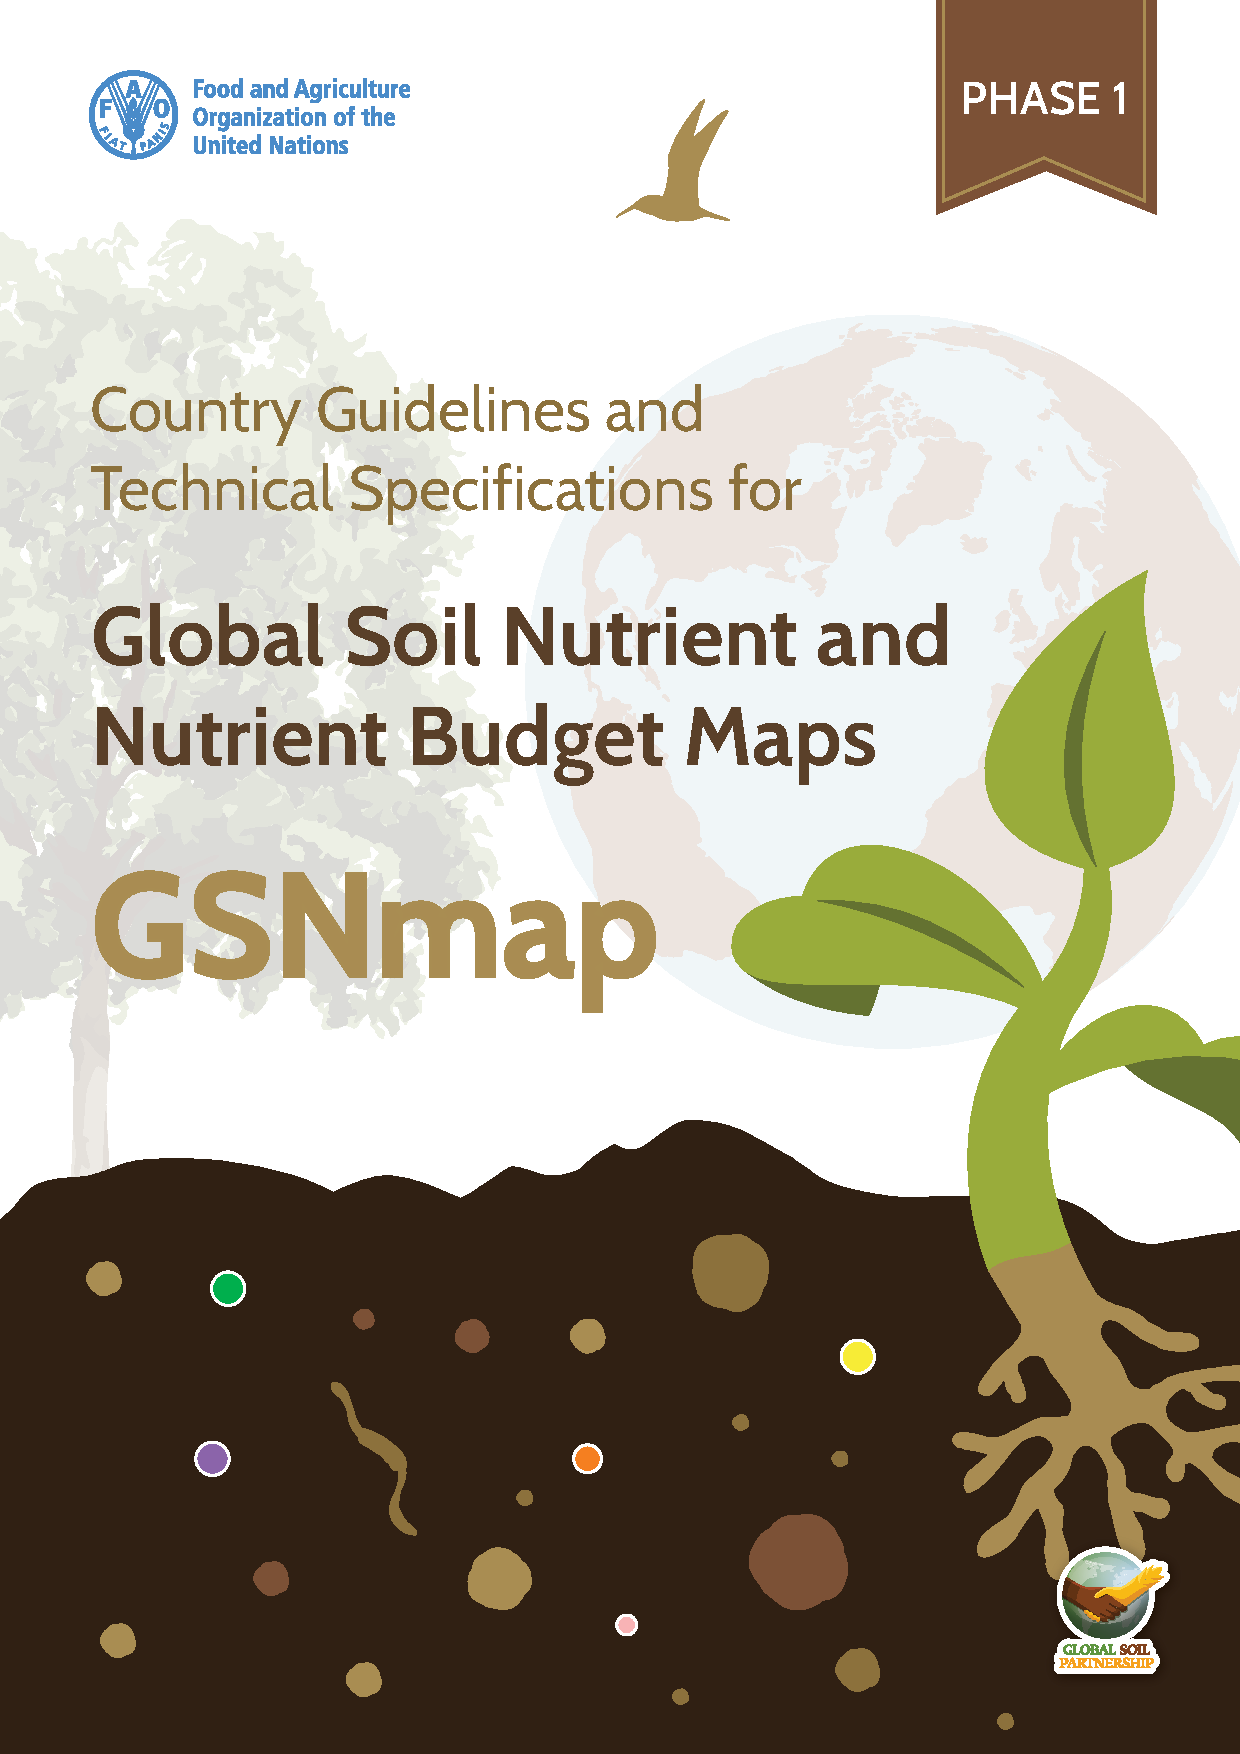
\includepdf{images/frontcover.pdf}
\afterpage{\blankpage}
\thispagestyle{empty}
\begin{titlepage}
    \begin{center}
        \vspace*{4cm}
        \Large

        \textcolor{astral}{\textbf{Country Guidelines on Digital Soil Mapping\\}}
        \vspace{0.5cm}
        \normalsize
        \vfill
        \noindent
        {\color{astral}\rule{\linewidth}{0.5mm} }

        Food and Agriculture Organization of the United Nations\\
	Rome, 2022
    \end{center}
\end{titlepage}
\includepdf{images/CB9015EN_Copyright Disclaimer_v2.pdf}


\frontmatter
\addtocontents{toc}{\protect\hypersetup{hidelinks}}   
\addtocontents{lof}{\protect\hypersetup{hidelinks}}
\addtocontents{lot}{\protect\hypersetup{hidelinks}}
\tableofcontents
\listoffigures
\listoftables
\nopagebreak[4]

\hypertarget{abbreviations-and-acronyms}{%
\chapter*{Abbreviations and acronyms}\label{abbreviations-and-acronyms}}
\addcontentsline{toc}{chapter}{Abbreviations and acronyms}

\begin{description}
\item[BD]
Bulk density
\item[CEC]
Cation exchange capacity
\item[CRAN]
Comprehensive R archive network
\item[DSM]
Digital soil mapping
\item[GEE]
Google Earth Engine
\item[GSP]
Global Soil Partnership
\item[INSII]
International Network of Soil Information Institutions
\item[ITPS]
Intergovernmental Technical Panel on Soils
\item[ME]
Mean error
\item[MAE]
Mean absolute error
\item[MEC]
Modelling efficiency coefficient
\item[NDVI]
Normalized difference in vegetation index
\item[QA/QC]
Quality assurance/quality check
\item[RMSE]
Root mean squared error
\item[SOC]
Soil organic carbon
\item[SOM]
Soil organic matter
\end{description}

\hypertarget{editors}{%
\chapter*{Editors}\label{editors}}
\addcontentsline{toc}{chapter}{Editors}

\emph{Prepared by:}\\
\textbf{Global Soil Partnership Secretariat}\\
Ronald Vargas\\

\hypertarget{contributors-and-reviewers}{%
\chapter*{Contributors and reviewers}\label{contributors-and-reviewers}}
\addcontentsline{toc}{chapter}{Contributors and reviewers}

\textbf{International Network of Soil Information Institutions}\\

\textbf{GSNmap working group}

\textbf{Fourth Intergovernmental Technical Panel on Soils}\\
Mr Guillermo A. Studdert (Argentina); Mr Braj Singh (Australia); Mr Igue Attanda Mouinou (Benin); Ms Lúcia Helena Cunha dos Anjos (Brazil); Mr Georges Martial Ndzana (Cameroon); \emph{Vicechair} Mr David Lobb (Canada); Mr Jin Ke (China); Mr Mohamed Abdel Wareth Mahmoud (Egypt); Mr Sheleme Beyene Jiru (Ethiopia); Mr Ravendra Naidu (Fiji); Ms Taina Pennanen (Finland); Ms Claire Chenu (France); Mr Ranjan Bhattacharyya (India); Mr Saeed Saadat (Iran); Ms Adele Muscolo (Italy); Ms Jeyanny Vijayanathan (Malaysia); Mr Jorge Dionisio Etchevers Barra (Mexico); Mr Matshwene Edwin Moshia (South Africa); \emph{Chair} Ms Rosa Maria Poch (Spain); Mr Harsha Kumara Kadupitiya (Sri Lanka); Mr Ghiath Ahmad Alloush (Syria);Ms Nyambilila Abdallah Amuri (Tanzania); Ms Nopmanee Suvannang (Thailand); Mr Gaius Eudoxie (Trinidad and Tobago); Mr Pete Smith (United Kingdom); Mr Michael Castellano (United States of America); Ms Deyanira Lobo (Venezuela)\\

\mainmatter

\hypertarget{presentation}{%
\chapter{Presentation}\label{presentation}}

\hypertarget{background-and-objectives}{%
\section{Background and objectives}\label{background-and-objectives}}

Soil nutrient availability can affect ecosystem carbon cycling, plant phenology, plant diversity and community composition, plant-herbivore and plant-soil-microbe interactions, as well as the structure of trophic food webs (\protect\hyperlink{ref-vanSundert2020}{Van Sundert \emph{et al.}, 2020}). Thus, the broad range of effects of nutrient availability also affects ecosystem functioning in face of global change, for instance the response of plants to elevated levels of CO\textsubscript{2} (\protect\hyperlink{ref-vicca2018}{Vicca \emph{et al.}, 2018}).

In the context of agriculture, nutrient availability modulates crop productivity and thus food production. However, the COVID-19 pandemic, current conflicts and devastating extreme weather events triggered by climate change jeopardise achieving sustainable development goal (SDG) 2 (Zero Hunger) by 2030. To date, a total number of around 2.3 billion people are affected by moderate and severe food insecurity (\protect\hyperlink{ref-FAO2022}{FAO and WHO, 2022}). Despite soil nutrient status and availability being vital to the provisioning of ecosystem services, globally-accessible and harmonised datasets on soil nutrient stocks and soil properties that govern nutrient availability are missing.

Therefore, the current global situation requires an increase of food production while preserving natural (soil) resources, lowering greenhouse gas emissions and optimising the use of goods such as fertilisers on agricultural sites (\protect\hyperlink{ref-eisenstein2020}{Eisenstein, undated}). Fertiliser prices more than doubled within one year and grain prices increased by around 25 percent (Jan.~2021 - Jan.~2022) (\protect\hyperlink{ref-ifpri2020}{Hebebrand, 2022}). With the start of the armed conflict in Ukraine in February 2022, this trend became more pronounced.
Growing food insecurity and rapidly increasing fertiliser prices underscore the urgent need for informed decision-making and optimised soil nutrient management. However, a large data gap exists in regards to soil nutrient stocks and soil properties that govern nutrient availability. Therefore, FAO's Global Soil Partnership (GSP) has launched the Global Soil Nutrient and Nutrient Budget map (GSNmap) initiative in an endeavour to provide harmonised and finely resolved soil nutrient data and information to stakeholders following a country-driven approach.
Up-to-date soil data on the status and spatial trends of soil nutrients and related soil attributes is key to guide policy-making to close yield gaps, and protect local natural resources. Therefore, locally-specific optimisation of soil nutrient and agricultural management are needed (\protect\hyperlink{ref-cunningham2013}{Cunningham \emph{et al.}, 2013}). The soil information collected in the GSNmap thereby serves as a cornerstone in delineating priority areas for action and thereby seizes the opportunity to reduce food insecurity, close yield gaps, and reduce environmental costs arising from mismanagement of soil nutrients and especially overfertilisation.

\hypertarget{global-soil-partnership}{%
\section{Global Soil Partnership}\label{global-soil-partnership}}

The Global Soil Partnership (GSP) was established in December 2012 as a mechanism to develop a strong interactive partnership and to enhance collaboration and generate synergies between all stakeholders to raise awareness and protect the world's soil resources. From land users to policymakers, one of the main objectives of GSP is to improve governance and promote sustainable management of soils. Since its creation, GSP has become an important partnership platform where global soil issues are discussed and addressed by multiple stakeholders at different levels.

The mandate of GSP is to improve governance of the planet's limited soil resources in order to guarantee productive agricultural soils for a food-secure world. In addition, it supports other essential soil ecosystem services in accordance with the sovereign right of each Member State over its natural resources. In order to achieve its mandate, GSP addresses six thematic action areas to be implemented in collaboration with its regional soil partnerships (Figure 1).

The area of work on Soil Information and Data (SID) of the GSP builds an enduring and authoritative global system (GloSIS) to monitor and forecast the condition of the Earth's soil resources and produce map products at the global level. The secretariat is working with the international network of soil data providers (INSII - International Network of Soil Information Institutions) to implement data related activities.

\hypertarget{country-driven-approach-and-tasks}{%
\section{Country-driven approach and tasks}\label{country-driven-approach-and-tasks}}

The GSNmap initiative will be jointly implemented by the International Network of Soil Information Institutions (INSII) and the GSP Secretariat. The process will be country-driven, involving and supporting all Member States in developing their national GSNmap data products. The GSNmap products will be developed following a two phase approach:

\begin{itemize}
\tightlist
\item
  Phase I: development of soil nutrient and associated soil property maps;
\item
  Phase II: quantification, analysis, projections of nutrient budgets for agricultural land use systems at national, regional and global scale.
\end{itemize}

These guidelines only concern GSNmap Phase I, while the guidelines for the GSNmap Phase II will be published in the fourth quarter of 2022.
Depending on national data availability and technical capacities, ad-hoc solutions will be developed by the GSNmap WG to support countries during the national GSNmap production and/or harmonisation phase. Where possible, GSP Secretariat will use publicly available data to gap-fill the areas which are not covered by the national submissions unless the country requests to be left blank on the GSNmap products.

\hypertarget{how-to-use-this-book}{%
\section{How to use this book}\label{how-to-use-this-book}}

The present document is a technical manual on the phase I of the GSNmap initiative. It provides the scientific background on the importance of soil nutrients and guidance on the digital soil mapping techniques to map nutrients and soil properties that govern nutrient availability. It also comprises a compendium with all necessary scripts to generate national GSNmaps. These scripts are described step-by-step in 4 steps that cover soil data preparation (Step 1), covariate download (Step 2), the mapping process itself (Step 3), and the automatic generation of national reports (Step 4). The general workflow is shown in Figure \ref{fig:steps}.

\begin{figure}
\includegraphics[width=28.12in]{images/Manual-Workflow} \caption{Overview of the steps to follow for the GSNmap generation.}\label{fig:steps}
\end{figure}

The chapters are structured as following:

\begin{itemize}
\tightlist
\item
  Chapter 1 provides general information about the GSNmap initiative as another activity of the GSP.
\item
  Chapter 2 focuses on the scientific state-of-the-art in terms of soil nutrients and soil nutrient mapping.
\item
  Chapter 3 and 4 introduce the software requirements and the concept of digital soil mapping.
\item
  Chapter 5 to 7 guide the reader through the nutrient mapping exercise of GSNmap Phase I providing step-by-step instructions.
\item
  Chapter 8 explains how the national GSNmaps are reported to the GSP.
\item
  Annex I serves as a repository for the complete scripts needed for the GSNmap.
\item
  Annex II provides alternative step-by-step instructions for the special case of soil data without point coordinates.
\end{itemize}

The GSNmap Technical Manual is structured as a practical document to be used by national experts in the endeavour to employ digital soil mapping techniques to generate national nutrient maps based on a common methodology. The concept of digital soil mapping presented here can however be also used in mapping exercises that focus on other soil properties and is therefore also relevant to scientists and digital soil mappers. The training material and the folders of the technical manual can be downloaded as .zip file here: \url{https://github.com/FAO-GSP/GSNmap-TM/archive/refs/heads/main.zip}. Alternatively, the GitHub repository can be cloned to your local device by using the following link: \url{https://github.com/FAO-GSP/GSNmap-TM.git}.

\hypertarget{soil-nutrients}{%
\chapter{Soil Nutrients}\label{soil-nutrients}}

\hypertarget{definition-of-soil-nutrients}{%
\section{Definition of soil nutrients}\label{definition-of-soil-nutrients}}

In theory, soil nutrients are defined as those chemical elements that are \emph{essential} to plant growth (\protect\hyperlink{ref-arnon1939}{Arnon and Stout, 1939}; \protect\hyperlink{ref-vonLiebig1841}{Liebig, 1841}). First, von Liebig (1841) declared nitrogen (N), sulphur (S), phosphorus (P), potassium (K), calcium (Ca), magnesium (Mg), silicon (Si), sodium (Na) and iron (Fe) as being essential. However, these findings lacked experimental research and were based on merely observational studies. Furthermore, if plant uptake is the only criteria for essentiality, the definition disregards the fact that plants also take up innecessary or even toxic elements.
Therefore, stricter criteria such as the one by Arnon and Stout (\protect\hyperlink{ref-arnon1939}{1939}) were defined. They postulated that three criteria need to be met for an \emph{essential mineral nutrients} (\protect\hyperlink{ref-mengel2012}{Mengel and Kirkby, 2012}):
1. Nutrient must be required by plants to complete their life cycle;
2. Nutrient must be irreplaceable; and
3. Nutrient must be involved in the plant metabolism.

Following this defintion to date the following nutrients would be considered essential for higher plants (\protect\hyperlink{ref-mengel2001}{Mengel \emph{et al.}, 2001}): carbon (C), hydrogen (H), oxygen (O), N, P, S, cobalt (Co), K, Ca, Mg, Fe, manganese (Mn), copper (Cu), Si, zinc (Zn), molybdenum (Mo), boron (B), chlorine (Cl), nickel (Ni), Na. However, Co, Si, Ni, and Na are not considered essential for all plants.

Other definitions used biochemical functions for classification purposes (\protect\hyperlink{ref-mengel2001}{Mengel \emph{et al.}, 2001}). Here, four nutrient groups are distinguished:
1. major constituents of organic material (C, H, O, N, S);
2. nutrients that are involved in esterification of alcohol groups (P, B, Si);
3. nutrients that establish an osmotic potential (ions) (K, Na, Ca, Mg, Mn, Cl); and
4. nutrients that enable electron transport (ions or chelates) (Fe, Cu, Zn, Mo).

Still, the most common classification of soil nutrients is based on the absolute quantities of an element that a plant takes up resulting in macro- and micronutrients (\protect\hyperlink{ref-mengel2012}{Mengel and Kirkby, 2012}). Despite being widely used, the definition has several shortcomings as also toxic elements can be taken up in greater quantities (e.g.~Al). Furthermore, the threshold definition between macro- and micronutrients is somewhat arbitrary (\protect\hyperlink{ref-mengel2012}{Mengel and Kirkby, 2012}).
It is important to point out that the discussion on how to accurately define \emph{essential} nutrients is ongoing as recent contribution to the topic show (\protect\hyperlink{ref-brown2022}{Brown, Zhao and Dobermann, 2022}). The generation of the GSNmaps is oriented by the recently published report on the state of the art of soils for nutrition (\protect\hyperlink{ref-symposium2022}{FAO, 2022}) and is shown in Table \ref{tab:nutrients}. It is based on the contribution of each element to the average plant content.

\label{tab:nutrients}Classification of major and micronutrients by FAO (2022).

Major nutrients

Micronutrients

N

Fe

P

Mn

K

Zn

Ca

Cu

Mg

B

S

Mo

Cl

\hypertarget{soil-properties-governing-nutrient-availability}{%
\section{Soil properties governing nutrient availability}\label{soil-properties-governing-nutrient-availability}}

The uptake of nutrients by plants is regulated in parts by the organism itself as for instance shoot growth is coupled with root growth (\protect\hyperlink{ref-wang2007}{Wang \emph{et al.}, 2007}). Still, soil properties mediate nutrient mobility and conditions at the plant-soil interface. The most important soil properties that determine nutrient availability are physicochemical properties such as soil pH, cation exchange capacity (CEC), soil texture, soil organic matter (SOM) content, and bulk density (BD).
Most nutrients are taken up in their ionized form (\protect\hyperlink{ref-robertson1999}{Robertson \emph{et al.}, 1999}). Therefore, the chemical characterization of the soil solution is key to understand nutrient dynamics and uptake.
Soil pH, as a measure of exchangeable hydrogen protons (H\textsuperscript{+}), is a crucial parameter to determine the acidity of the soil solution that can inhibit or mediate nutrient uptake. For instance, very low pH values of around 4 decreased the uptake of (basic) cations such as Ca or Mg by paddy rice, wheat, corn, common bean and cowpea whereas lower pH values favoured the uptake of Zn, Fe, and Mn. At higher pH values the uptake of cations was enhanced (\protect\hyperlink{ref-fageria2014}{Fageria and Knupp, 2014}).
The CEC, as a measure of exchangeable cations (e.g K\textsuperscript{+}, Mg\textsuperscript{2+}, Ca\textsuperscript{2+}, etc.) available in the soil solution and attached to soil particles is a complementary parameter of nutrient availability in soils (\protect\hyperlink{ref-robertson1999}{Robertson \emph{et al.}, 1999}). The CEC informs on the capacity of soils to retain positively charged nutrients (basic cations) and thus gives information on how strong a soil can buffer subsequent acidification. This retention and buffer capacity is strongly linked to soil texture. High clay contents usually lead to higher CEC and thus higher cation retention. Conversely, sandy textured soils strongly rely on soil organic matter (SOM) content that has high CEC to retain cations.
SOM content further augments aeration of soils due to its low density and provides high specific surface area to retain nutrients.
Finally, BD is key to nutrient availability as it governs facilitates or inhibits root growth and thus nutrient uptake by plants. Due to its impact on soil porosity, BD also governs microbial activity (through aeration) and water infiltration that defines nutrient mobility.

\hypertarget{setting-up-the-software-environment}{%
\chapter{Setting-up the software environment}\label{setting-up-the-software-environment}}

This chapter provides an overview on the software required to map soil nutrients and associated soil properties. The tools are open source and can be downloaded and installed by users following the steps that are described here. The instructions given are for Microsoft Windows operational systems. Instructions for other operational systems (e.g.~Linux Flavours, MacOS) can be found through free online resources.

\hypertarget{use-of-r-rstudio-and-r-packages}{%
\section{Use of R, RStudio and R Packages}\label{use-of-r-rstudio-and-r-packages}}

\textbf{R} is a language and environment for statistical computing created in 1992. It provides a wide variety of statistical (e.g.~linear modeling, statistical tests, time-series, classification, clustering, etc.) and graphical methods, and has been constantly extended by an exceptionally active user community.

\hypertarget{obtaining-and-installing-r}{%
\subsection{Obtaining and installing R}\label{obtaining-and-installing-r}}

Installation files and instructions can be downloaded from the Comprehensive R Archive Network (CRAN).

\begin{enumerate}
\def\labelenumi{\arabic{enumi}.}
\tightlist
\item
  Go to the following link \url{https://cran.r-project.org/} to download and install \textbf{R}.
\item
  Pick an installation file for your operational system.
\item
  Choose the ``\emph{base}'' distribution of R (particularly if it is the first time you install \textbf{R}).
\item
  Download the R installation file and open the file on your device.
\item
  Follow the installation instructions.
\end{enumerate}

\hypertarget{obtaining-and-installing-rstudio}{%
\subsection{Obtaining and installing RStudio}\label{obtaining-and-installing-rstudio}}

Beginners will find it very hard to start using \textbf{R} because it has no Graphical User Interface (GUI). There are some GUIs which offer some of the functionality of \textbf{R}. \textbf{RStudio} makes \textbf{R} easier to use. It includes a code editor, debugging and visualization tools. Similar steps need to be followed to install \textbf{RStudio}.

\begin{enumerate}
\def\labelenumi{\arabic{enumi}.}
\tightlist
\item
  Go to \url{https://www.rstudio.com/products/rstudio/download/} to download and install \textbf{RStudio}'s open source edition.
\item
  On the download page, \emph{RStudio Desktop, Open Source License} option should be selected.
\item
  Pick an installation file for your platform.
\item
  Follow the installation instruction on your local device.
\end{enumerate}

\begin{figure}
\includegraphics[width=18.97in]{images/2_RStudio-interface} \caption{R Studio interface.}\label{fig:Rstudio}
\end{figure}

The \textbf{RStudio} interface is structured by four compartments (see Fig. \ref{fig:Rstudio}). The code editor is located in the upper left. Scripts that contain codes are displayed here. New scripts can be opened by clicking on the left most \emph{New} button in the quick access tool bar (highlighted in green). Lines of code can be executed by clickinig on \emph{Run} (highlighted in blue) or by pressing \emph{ctrl + enter} on your keyboard.
The output of scripts or lines of code that are executed is displayed in the window below the code editor: the console (bottom left). This part of the interface corresponds to the \textbf{R} software that were installed previously.
When working in \textbf{R}, it is central to work with so-called objects (for instance vectors, dataframes or matrices). These objects are saved in the global environment that is displayed in the top right panel.
Finally, the \textbf{R} software offers a broad range of powerful tools for visualisation purposes. Graphs or maps that are generated by scripts/codes, are displayed in the bottom right panel.

\hypertarget{getting-started-with-r}{%
\subsection{Getting started with R}\label{getting-started-with-r}}

\begin{itemize}
\tightlist
\item
  \textbf{R} manuals: \url{http://cran.r-project.org/manuals.html}
\item
  Contributed documentation: \url{http://cran.r-project.org/other-docs.html}
\item
  Quick-\textbf{R}: \url{http://www.statmethods.net/index.html}
\item
  Stackoverflow \textbf{R} community: \url{https://stackoverflow.com/questions/tagged/r}
\end{itemize}

\hypertarget{r-packages}{%
\section{R packages}\label{r-packages}}

When you download \textbf{R}, you get the basic \textbf{R} system which implements the \textbf{R} language. \textbf{R} becomes more useful with the large collection of packages that extend the basic functionality of it. \textbf{R} packages are developed by the \textbf{R} community.

refer to:
* \emph{tidyverse} book (R for data science)
* \emph{caret} (broad range of statistical learning functions)
* \emph{R spatial}: \url{https://rspatial.org/} (R packages for spatial data operations)

The primary source for \textbf{R} packages is \href{https://cran.r-project.org/}{CRAN's} official website, where currently about 12,000 available packages are listed. For spatial applications, various packages are available. You can obtain information about the available packages directly on CRAN with the `available.packages()' function. The function returns a matrix of details corresponding to packages currently available at one or more repositories. An easier way to browse the list of packages is using the \href{https://cran.r-project.org/web/views/}{\emph{Task Views}} link, which groups together packages related to a given topic.

Packages come along with extensive documentation that is very helpful to understand and solve error messages. To access information on functions or packages, type ``?{[}Package or Function name{]}'' in the console. The information on the package and/or function can then be accessed in the bottom right panel under ``Help'' (see Fig. \ref{fig:Rstudio}). In addition to that, the \emph{R documentation} website (\url{https://www.rdocumentation.org/}) provides more extensive help and gives clear overviews on all functions comprised in a certain package.

\hypertarget{gee---google-earth-engine}{%
\section{GEE - google earth engine}\label{gee---google-earth-engine}}

Google earth engine (GEE) provides a large range of remote sensing datasets for users. It allows to use the GEE code editor to run computations using the google servers. The high computational power of these servers enables users with limited computational caapacities to run complex calculations.
A user account must be created to use the code editor. This step can take some time. Once the account is validated, scripts can be written in the code editor using the Javascript language. An extensive array of instructions and guides are available on the platform. Alternatively, the Python language can be used to interact with the data.

The code editor interface is structured by three panels and a map viewer (see Fig. \ref{fig:GEE}). The left panel is structured in ``Scripts'', ``Docs'', and ``Assets''. Under ``Scripts'' users can organize and save the scripts they wrote for specific purposes. ``Docs'' provides further information on so-called ``server-side'' functions that can be used to manipulate the data. Finally, in ``Assets'' users can upload own spatial data in common formats such as shapefiles (.shp) or raster files (.tif).
The middle panel contains the scripts that can be run by clicking on the ``Run'' button.
The right panel is composed of three functionalities. The ``Inspector'' provides basic information on a pixel of a layer displayed in the map below. The information consists of longitude, latitude, and - if layers are loaded - values of the pixel. The ``Console'' is the place where certain commands expressed in the code are shown. The most common expressions shown here are print() commands or figures derived from the loaded data. Finally, the ``Tasks'' button shows all tasks that were formulated in the code/script and are to be submitted to the server for computation. Once a task is submitted, the user has to click on the ``Run'' button appearing in the ``Tasks'' section to submit the task to the server.
In addition to that, the data catalog can be accessed via the search bar on the top of the page. Here, key information on the available datasets, origin, resolution and related publications can be found.

\begin{figure}
\includegraphics[width=26.69in]{images/2.1_GEE_codeeditor} \caption{Google Earth Engine code editor.}\label{fig:GEE}
\end{figure}

The upload of \emph{assets} in particular shapefiles with the area of interest (AOI) is often a key step to extract only the necessary information from a dataset. To upload a dataset, once has to right-click on ``Assets'' in the right panel and then on the red ``New'' button in the code editor interface (see Fig. \ref{fig:asset}). After selecting the file format of file, a second window opens.

\begin{figure}
\includegraphics[width=23.42in]{images/2.2_upload-assets-1} \caption{Select files and filetype to be uploaded as GEE assets.}\label{fig:asset}
\end{figure}

Here the source file needs to be selected from the respective folder and a folder in the GEE environment has to be selected under ``Asset ID''. After that, the user right-clicks on ``Upload'' in the bottom right of the window (see Fig. \ref{fig:upload}). In the right panel under ``Tasks'' appears the uploading task that is executed. Once this process is finished, a tick mark appears and after refreshing the ``Assets'' panel on the left, the user can see the uploaded shapefile.

\begin{figure}
\includegraphics[width=7.56in]{images/2.3_upload-assets-2} \caption{Upload interface.}\label{fig:upload}
\end{figure}

\hypertarget{rgee---extension-to-use-google-earth-engine-in-r}{%
\section{rgee - Extension to use google earth engine in R}\label{rgee---extension-to-use-google-earth-engine-in-r}}

To generate the GSNmap, the user is going to use an R package to interact with the GEE environment. The \emph{rgee} package enables users to interact with the GEE servers using the R language (\protect\hyperlink{ref-rgee}{Aybar, 2022}). The package makes use of the Python language to interact with GEE. The package can be downloaded easily either directly from the GitHub repository or via CRAN.

The prerequisite to have access to GEE is to create a user account on \url{https://earthengine.google.com/}. Once you have a GEE account, it is necessary to install the rgee package on your machine. After installing and loading the package to your session in \textbf{R studio}, it is necessary to install the so-called ``\emph{Miniconda}'' command prompt which acts as a Python interpreter mediating between R and GEE. The `ee\_install()' function automatically downloads and install all the software that is needed.

\begin{Shaded}
\begin{Highlighting}[]
\CommentTok{\# install package}
\FunctionTok{install.packages}\NormalTok{(}\StringTok{"rgee"}\NormalTok{)}

\CommentTok{\# load rgee package}
\FunctionTok{library}\NormalTok{(rgee)}

\CommentTok{\# install miniconda and other dependencies}
\FunctionTok{ee\_install}\NormalTok{(}\AttributeTok{py\_env =} \StringTok{"rgee"}\NormalTok{) }
\end{Highlighting}
\end{Shaded}

Once the dependencies are installed, it is necessary to initialize rgee by providing the user credentials of the created GEE account. The ee\_Initialize command must be run every time rgee is used.

\begin{Shaded}
\begin{Highlighting}[]
\CommentTok{\# Initialize Google Earth Engine! (you need to create a user account)}
\FunctionTok{ee\_Initialize}\NormalTok{()}
\end{Highlighting}
\end{Shaded}

In case problems arise during the installation, the following functions may be helpful to clear user credentials or clean the python environment created with the ee\_install() command. In first place, it is recommendable to consult the rgee documentation website (\url{https://r-spatial.github.io/rgee/articles/rgee01.html}) to get more detailed information on the installation procedure and possibilities for problem solving.

\begin{Shaded}
\begin{Highlighting}[]
\CommentTok{\# Useful functions}

\CommentTok{\#ee\_check() \# check the dependencies that do not belong to R}
\CommentTok{\#ee\_clean\_credentials() \# to remove the user credentials}
\CommentTok{\#ee\_clean\_pyenv() \# Delete variables of the system}
\end{Highlighting}
\end{Shaded}

\hypertarget{digital-soil-mapping}{%
\chapter{Digital Soil Mapping}\label{digital-soil-mapping}}

\hypertarget{principles}{%
\section{Principles}\label{principles}}

Digital soil mapping (DSM) is a methodological framework to create soil attribute maps on the basis of the quantitative relationships between spatial soil databases and environmental covariates. The quantitative relations can be modelled by different statistical approaches, most of them considered machine learning techniques. Environmental covariates are spatially explicit proxies of soil-forming factors that are employed as predictors of the geographical distribution of soil properties. The methodology has evolved from the theories of soil genesis developed by Dokuchaev (\protect\hyperlink{ref-Dokuchaev1883}{1883}) in his work the Russian Chernozems, which later were formalised by Jenny (\protect\hyperlink{ref-Jenny1941}{1941}) with the equation of the soil-forming factors. The conceptual equation of soil-forming factors has been updated by McBratney, Santos and Minasny (\protect\hyperlink{ref-McBratney2003}{2003}) as follow:

\begin{equation} 
  S = f\left(s,c,o,r,p,a,n\right)
  \label{eq:scorpan}
\end{equation}

Where \(S\) is the soil classes or attributes (to be modelled) as a function of ``\(s\)'' as other soil properties, ``\(c\)'' as climatic properties, ``\(o\)'' as organisms, including land cover and human activity, ``\(r\)'' as terrain attributes, ``\(p\)'' as parent material, ``\(a\)'' as soil age, and ``\(n\)'' as the geographic position.

\hypertarget{environmental-covariates}{%
\section{Environmental covariates}\label{environmental-covariates}}

There is an constantly increasing range of global datasets that can be used as environmental covariates. Covariates usually provide information on the soil forming factors. However, they are always only an approximation to the reality in the field. The selection of covariates aims to give the most accurate picture of the reality and thus complement each other. In the case of climatic covariates for instance, useful covariates should not only cover the long-term mean annual temperature or precipitation over an climatic reference period (30 years) but also inform about seasonal patterns or even diurnal variability. Still, when selecting covariates one has to keep in mind that there is a trade-off between accurate representation of reality and overfitting the model used for modelling.

\hypertarget{machine-learning-techniques}{%
\section{Machine learning techniques}\label{machine-learning-techniques}}

A broad range of modelling approaches coexist in order to establish quantitative relationships between environmental covariates and the target soil properties to be mapped. The plethora of methods cannot be listed here as it was summarised in multiple review papers (\protect\hyperlink{ref-khaledian2020}{Khaledian and Miller, 2020}; \protect\hyperlink{ref-lamichhane2019}{Lamichhane, Kumar and Wilson, 2019}; \protect\hyperlink{ref-ma2019}{Ma \emph{et al.}, 2019}; \protect\hyperlink{ref-padarian2019}{Padarian, Minasny and McBratney, 2019}; \protect\hyperlink{ref-wadoux2020}{Wadoux, Minasny and McBratney, 2020}).
Traditionally, multiple linear regression models can be used to quantify the relationships which continues to be the most applied mapping method to map for instance soil organic carbon (\protect\hyperlink{ref-lamichhane2019}{Lamichhane, Kumar and Wilson, 2019}). In addition to that, regression Kriging methods combine linear regressions and an stochastic interpolation of the regression residuals based on their spatial autocorrelation (\protect\hyperlink{ref-yigini2018}{Yigini \emph{et al.}, 2018}).
However, machine learning algorithms with more flexible assumptions, i.e.~non-linear relationships, have become more and more popular as the mapping performance was substantially improved and the versatility of the algorithms can be detect more complex relationships.
Among the most commonly used non-linear machine learning models is random forest (\protect\hyperlink{ref-Breiman2001}{Breiman, 2001}). The random forest algorithm splits a dataset into subsets and uses a random selection of covariates (predictors) to identify homogeneous groups. The procedure of classifying is repeated many times and in the end the prediction is averaged. Finally, quantile regression forests (QRF) derive from random forest models (\protect\hyperlink{ref-Meinshausen2006}{Meinshausen, 2006}). The benefit of QRF is the ability to predict not only the mean of the prediction but also to provide more information on the uncertainty and probability distribution.

\hypertarget{mapping-of-soil-nutrients-and-associated-soil-attributes}{%
\section{Mapping of soil nutrients and associated soil attributes}\label{mapping-of-soil-nutrients-and-associated-soil-attributes}}

DSM has been used to produce maps of soil nutrients at regional to continental scales. For instance, Hengl \emph{et al.} (\protect\hyperlink{ref-Hengl2017}{2017}) predicted 15 soil nutrients at a 250 m resolution in Africa using a random forest model (\protect\hyperlink{ref-wright2016}{Wright, Ziegler and König, 2016}). The soil nutrient observations were collected for topsoils at locations that were unevenly distributed over the continent and a set of spatially-explicit environmental covariates including soil properties. In 2021, the map resolution was increased to 30 x 30 m by using additional soil samples (\protect\hyperlink{ref-hengl2021}{Hengl \emph{et al.}, 2021}).
In Europe maps of chemical soil properties, including macronutrients like potassium and phosphorus, were mapped based on a gaussian process regression using the LUCAS soil database (\protect\hyperlink{ref-ballabio2019}{Ballabio \emph{et al.}, 2019}).
Global efforts to map nutrients in a harmonised way are suffering of constraints due to limited availability of appropriate soil data. The country-driven approach of the GSP has therefore the potential to improve data availability through the country-driven approach as it uses largely unexplored soil data, a harmonised mapping approach combined with national expertise on the regional soil resources. Therefore, in this technical manual, we present a DSM framework to map soil nutrients and associated properties using soil observations with latitude and longitude coordinates (point-support) (Figure \ref{fig:workflow1}).

\begin{figure}
\includegraphics[width=16.1in]{images/workflow_county_data} \caption{Digital soil mapping approach for point-support data. Circles are the steps.}\label{fig:workflow1}
\end{figure}

\hypertarget{step-1-soil-data-preparation}{%
\chapter{Step 1: soil data preparation}\label{step-1-soil-data-preparation}}

\hypertarget{format-requirements-and-pre-processing-of-soil-data}{%
\section{Format requirements and pre-processing of soil data}\label{format-requirements-and-pre-processing-of-soil-data}}

Soil data consist of measurement at a specific geographical location, time and soil depth. Therefore, it is necessary to arrange the data following the format shown in Table \ref{tab:data1}.

\label{tab:data1}Example format of a database.

Profile ID

Horizon ID

Lat

Long

Year

Top

Bottom

cec

ph

clay

silt

sand

soc

bd

1

1\_1

12.12346

1.123456

2018

0

20

15

6.5

35

58

7

3.4

1.31

1

1\_2

12.12346

1.123456

2018

20

40

19

7.1

42

48

10

2.1

1.32

2

2\_1

23.12346

2.123456

2019

0

30

14

5.5

12

53

35

2.9

1.39

{Note: }

Profile ID = unique profile identifier, Horizon ID = unique layer identifier, Lat = latitude in decimal degrees, Long = longitude in decimal degrees, Year = sampling year, Top = upper limit of the layer in cm, Bottom = lower limit of the layer in cm, cec = Cation Exchange Capacity (cmol\_c/kg), ph = pH in water, clay = Clay (g/100g soil), silt = Silt (g/100g soil), sand = Sand ((g/100g soil), soc = Soil Organic Carbon (g/100g soil), bd = Bulk Density (g/cm3).

In this chapter, step-by-step instructions are given on how to carry out all these steps in \textbf{RStudio}. Instructions are given on how to:

\begin{enumerate}
\def\labelenumi{\arabic{enumi}.}
\tightlist
\item
  Generate user-defined variables,
\item
  Set the working directory and load necessary packages,
\item
  Import national data to \textbf{R Studio}
\item
  Select useful columns
\item
  Perform a quality check of the data
\item
  Estimate bulk density using PTF
\item
  Harmonize soil layers (using splines)
\item
  Plot and save the formatted soil data
\end{enumerate}

Thus, the instructions also serve as a very basic introduction to the functioning of \textbf{R} and \emph{RStudio}. Still, in case for further information there is a vast amount of websites that offer help and or information on \textbf{R} and \emph{RStudio}.

Soil data usually require a pre-processing step to solve common issues such as, arranging the data format, fixing soil horizon depth consistency, detecting unusual soil property measurements, among others issues. Here, common issues and examples are given on how to carry out some basic data handling steps in \emph{RStudio}. Next to in-built base R functions, the tidyverse package(s) offer a great help for data handling in \textbf{R}.

\begin{Shaded}
\begin{Highlighting}[]
\CommentTok{\# Select columns}
\NormalTok{coord }\OtherTok{\textless{}{-}}\NormalTok{ data }\SpecialCharTok{\%\textgreater{}\%} \FunctionTok{select}\NormalTok{(ID, x, y, om, ph)}

\CommentTok{\# Filter}

\CommentTok{\# remove NAs}


\CommentTok{\# remove duplicates}





\CommentTok{\# rename}

\CommentTok{\# change class of columns / check for class}
\end{Highlighting}
\end{Shaded}

Once the original dataset is clean and consistent, data harmonisation is needed to produce synthetic horizons (such as 0--30 cm layer), as well as to make compatible measurements from different lab methods. Horizon harmonisation will be done with the mass preserving spline function (\protect\hyperlink{ref-Bishop1999}{Bishop, McBratney and Laslett, 1999}; \protect\hyperlink{ref-Malone2009}{Malone \emph{et al.}, 2009}) fitted to each individual soil profile, which requires more than a layer per profile.

\hypertarget{study-area-and-soil-data}{%
\section{Study area and soil data}\label{study-area-and-soil-data}}

The study area is located in the southeast of the Pampas Region, in Argentina, from the foothills of the Ventania and Tandilia hill systems, until the southern coasts of the Buenos Aires Province.
To illustrate the different processes of this Technical Manual, we use three datasets from this region:

\begin{itemize}
\tightlist
\item
  Gereferenced topsoil data
\item
  Non-georreferenced topsoil data
\item
  Soil profile data
\end{itemize}

\hypertarget{georeferenced-topsoil-data}{%
\subsection{Georeferenced topsoil data}\label{georeferenced-topsoil-data}}

These data were collected in 2011 by the National Institute of Agriculture Technology and Faculty of Agricultural Science of the National University of Mar del Plata (Unidad Integrada INTA-FCA) to map the status of soil nutrients in the Argentinian Pampas (\protect\hyperlink{ref-sainz2019}{Sainz Rozas \emph{et al.}, 2019}). The dataset is a subset with 118 locations of topsoil samples (0-20 cm) that contains measurements of Organic Matter (om), P Bray (p\_bray), pH (ph), and K (k) (Table \ref{tab:table2}) and is shown in the following map as points. This dataset is used in \href{https://fao-gsp.github.io/GSNmap-TM/step-3-mapping-continuous-soil-properties.html\#step-3-mapping-continuous-soil-properties}{Chapter 7} for mapping K.

\label{tab:table2}Dataset with coordinates for mapping nutrients.

LabID

x

y

om

ph

p\_bray

k

51

-61.51282

-37.37646

4.03

6.50

20.40

852.2

60

-57.84725

-37.85136

5.53

6.05

10.52

769.6

64

-58.87620

-38.54000

4.85

6.30

15.87

992.4

67

-60.30394

-38.45300

3.13

6.30

20.85

740.2

68

-60.39772

-38.51567

2.92

6.16

13.54

724.8

69

-60.41442

-38.52914

2.15

6.65

46.17

699.0

74

-60.00556

-38.76500

4.12

6.27

20.94

518.6

75

-60.10750

-38.76472

4.24

5.84

26.82

450.2

77

-60.17139

-38.79278

3.35

6.57

22.56

858.8

78

-60.03111

-38.74611

3.53

6.49

20.09

662.9

Only the ten first rows are shown.

\begin{Shaded}
\begin{Highlighting}[]
\FunctionTok{library}\NormalTok{(tidyverse)}
\FunctionTok{library}\NormalTok{(sf)}
\FunctionTok{library}\NormalTok{(mapview)}

\FunctionTok{mapviewOptions}\NormalTok{(}\AttributeTok{fgb =} \ConstantTok{FALSE}\NormalTok{)}
\NormalTok{data }\OtherTok{\textless{}{-}} \FunctionTok{read\_csv}\NormalTok{(}\StringTok{"Digital{-}Soil{-}Mapping/01{-}Data/data\_with\_coord.csv"}\NormalTok{)}
\NormalTok{s }\OtherTok{\textless{}{-}} \FunctionTok{st\_as\_sf}\NormalTok{(data, }\AttributeTok{coords =} \FunctionTok{c}\NormalTok{(}\StringTok{"x"}\NormalTok{, }\StringTok{"y"}\NormalTok{), }\AttributeTok{crs =} \DecValTok{4326}\NormalTok{)}
\FunctionTok{mapview}\NormalTok{(s, }\AttributeTok{zcol =} \StringTok{"p\_bray"}\NormalTok{, }\AttributeTok{cex =} \FloatTok{2.5}\NormalTok{, }\AttributeTok{lwd =} \DecValTok{0}\NormalTok{)}
\end{Highlighting}
\end{Shaded}

\hypertarget{non-georeferenced-topsoil-data}{%
\subsection{Non-georeferenced topsoil data}\label{non-georeferenced-topsoil-data}}

The second dataset consist of topsoil samples (0-20cm) of P Bray (p\_bray) without geographical coordinates collected during 2005 by Sainz Rozas, Echeverria and Angelini (\protect\hyperlink{ref-sainz2011}{2011}) to map the status of soil nutrients in the Argentinian Pampas. Each sample is linked to an administrative unit (Partido) of the Buenos Aires Province (Table \ref{tab:table3}). This dataset is used in \href{https://fao-gsp.github.io/GSNmap-TM/annex-ii-mapping-without-point-coordinates.html}{Annex III: Mapping without point coordinates}

\label{tab:table3}Dataset with coordinates for mapping nutrients.

Partido

Cod\_Prov

Cod\_Part

stratum

p\_bray

Azul

06

049

6049

8.0

Azul

06

049

6049

13.9

Azul

06

049

6049

5.7

Azul

06

049

6049

8.4

Azul

06

049

6049

8.8

San Cayetano

06

742

6742

11.1

San Cayetano

06

742

6742

12.7

San Cayetano

06

742

6742

5.0

San Cayetano

06

742

6742

6.6

San Cayetano

06

742

6742

7.9

Only ten rows are shown.

The following map shows the districts with colours according to the sample size (n).

\begin{Shaded}
\begin{Highlighting}[]
\FunctionTok{library}\NormalTok{(tidyverse)}
\FunctionTok{library}\NormalTok{(sf)}
\FunctionTok{library}\NormalTok{(mapview)}
\FunctionTok{mapviewOptions}\NormalTok{(}\AttributeTok{fgb =} \ConstantTok{FALSE}\NormalTok{)}
\NormalTok{data }\OtherTok{\textless{}{-}} \FunctionTok{read\_csv}\NormalTok{(}\StringTok{"Digital{-}Soil{-}Mapping/01{-}Data/Buenos\_Aires\_sur\_P\_Bray.csv"}\NormalTok{)}
\NormalTok{district }\OtherTok{\textless{}{-}} \FunctionTok{st\_read}\NormalTok{(}\StringTok{"Digital{-}Soil{-}Mapping/01{-}Data/district.shp"}\NormalTok{, }\AttributeTok{quiet =}\NormalTok{ T)}
\FunctionTok{mapview}\NormalTok{(district, }\AttributeTok{zcol =} \StringTok{"n"}\NormalTok{, }\AttributeTok{lwd =} \DecValTok{0}\NormalTok{)}
\end{Highlighting}
\end{Shaded}

\hypertarget{soil-profile-data}{%
\subsection{Soil profile data}\label{soil-profile-data}}

Finally, the third dataset belongs to the Soil Information System of Argentina (\href{http://sisinta.inta.gob.ar/}{SISINTA}, Olmedo, Rodriguez and Angelini (\protect\hyperlink{ref-Olmedo2017}{2017})) which contains soil profiles collected from the sixties to recently years for soil survey purposes. The data can be fetched using the package \href{https://github.com/INTA-Suelos/SISINTAR\#readme}{SISINTAR}. Table \ref{tab:table4} shows a subset of the data, and the map presents the distribution of soil profiles for the study area. This dataset is used in this chapter to illustrate the preprocessing steps required for data that come from soil profiles.

\label{tab:table4}Soil profile dataset.

id\_prof

id\_hor

x

y

date

top

bottom

ph\_h2o

k

soc

51

28706

-60.35188

-38.80600

1986-10-28

0

15

6.5

1.5

2.59

51

28707

-60.35188

-38.80600

1986-10-28

15

25

6.5

1.7

2.46

51

28708

-60.35188

-38.80600

1986-10-28

25

52

6.5

0.8

1.28

51

28709

-60.35188

-38.80600

1986-10-28

52

57

NA

NA

NA

154

28425

-58.67430

-38.20796

1982-10-07

0

14

6.0

2.2

3.62

154

28426

-58.67430

-38.20796

1982-10-07

14

26

6.0

1.9

2.84

154

28427

-58.67430

-38.20796

1982-10-07

26

44

6.4

2.5

1.06

154

28428

-58.67430

-38.20796

1982-10-07

44

56

6.7

2.2

0.46

154

28429

-58.67430

-38.20796

1982-10-07

56

105

6.5

1.8

0.16

197

28588

-60.45918

-38.36285

1986-09-26

0

13

5.9

2.8

3.35

Only ten rows are shown.

\begin{Shaded}
\begin{Highlighting}[]
\FunctionTok{library}\NormalTok{(tidyverse)}
\FunctionTok{library}\NormalTok{(sf)}
\FunctionTok{library}\NormalTok{(mapview)}
\FunctionTok{mapviewOptions}\NormalTok{(}\AttributeTok{fgb =} \ConstantTok{FALSE}\NormalTok{)}
\NormalTok{data }\OtherTok{\textless{}{-}} \FunctionTok{read\_csv}\NormalTok{(}\StringTok{"Digital{-}Soil{-}Mapping/01{-}Data/soil\_profile\_data.csv"}\NormalTok{)}
\NormalTok{s }\OtherTok{\textless{}{-}}\NormalTok{ data }\SpecialCharTok{\%\textgreater{}\%} \FunctionTok{filter}\NormalTok{(top}\SpecialCharTok{==}\DecValTok{0}\NormalTok{)}
\NormalTok{s }\OtherTok{\textless{}{-}} \FunctionTok{st\_as\_sf}\NormalTok{(s, }\AttributeTok{coords =} \FunctionTok{c}\NormalTok{(}\StringTok{"x"}\NormalTok{, }\StringTok{"y"}\NormalTok{), }\AttributeTok{crs =} \DecValTok{4326}\NormalTok{)}
\FunctionTok{mapview}\NormalTok{(s, }\AttributeTok{zcol =} \StringTok{"k"}\NormalTok{, }\AttributeTok{cex =} \FloatTok{2.5}\NormalTok{, }\AttributeTok{lwd =} \DecValTok{0}\NormalTok{)}
\end{Highlighting}
\end{Shaded}

\hypertarget{preparatory-steps}{%
\section{Preparatory steps}\label{preparatory-steps}}

Now, let's open \emph{RStudio}. Whenever starting to work on a project or task, it is necessary to set the \emph{working directory} (WD). The WD is the folder path that is used by \textbf{R} to save the output, for instance a plot or a table that was generated while working in \textbf{R}. Thus, the WD is central since it dictates where the files and calculations can be found afterwards. As it is so important, there are multiple ways of setting the WD. One option is to right click on `Session' menu \textgreater{} `Set working directory \ldots{}' and select either `To Source File Location' (then the WD corresponds to the file path where the Script is saved to) or `Choose Directory\ldots{}'. Then, the user can browse to the folder that should be the WD.
In this manual we propose an alternative way that allows for more customization and flexibility since sometimes multiple WDs are needed to for instance save the final map in a different folder than the covariates. Therefore, we assign the file path that represents the WD file path to an \textbf{R} object. This is done by defining a character value (in this case the file path) on the right side of the arrow (\texttt{\textless{}-}) and name the \textbf{R} object on the left side (wd) (see code). Once this is done we use the function `setwd()' to set the WD to the file path that is specified in the object \texttt{wd}.

Before working on specific tasks in \textbf{R}, it is necessary to load the packages that contain the functions that are going to be used. Before one can load packages, they need to be installed. There are many ways to do this, yet the most common way is to call the function \texttt{install.packages()}. For instance, to install the \texttt{terra} package, one has to write \texttt{install.packages("terra")}. This installs the package from CRAN. However, there are a few exceptions where development versions of R packages are required. In these instances additional packages such as \texttt{devtools} or \texttt{remotes} are needed (see example in code below). These packages are then able to install packages from for instance GitHub repositories.

\begin{Shaded}
\begin{Highlighting}[]
\CommentTok{\# 0 {-} User{-}defined variables ===================================================}
\NormalTok{wd }\OtherTok{\textless{}{-}} \StringTok{\textquotesingle{}C:/Users/hp/Documents/GitHub/Digital{-}Soil{-}Mapping\textquotesingle{}}
\CommentTok{\#wd \textless{}{-} "C:/GIT/Digital{-}Soil{-}Mapping"}

\CommentTok{\# 1 {-} Set working directory and load necessary packages ========================}
\FunctionTok{setwd}\NormalTok{(wd) }\CommentTok{\# change the path accordingly}

\FunctionTok{library}\NormalTok{(tidyverse) }\CommentTok{\# for data management and reshaping}
\FunctionTok{library}\NormalTok{(readxl) }\CommentTok{\# for importing excel files}
\FunctionTok{library}\NormalTok{(mapview) }\CommentTok{\# for seeing the profiles in a map}
\FunctionTok{library}\NormalTok{(sf) }\CommentTok{\# to manage spatial data (shp vectors) }

\CommentTok{\# install.packages("devtools") }
\CommentTok{\# devtools::install\_bitbucket("brendo1001/ithir/pkg") \#install ithir package}
\FunctionTok{library}\NormalTok{(ithir) }\CommentTok{\# for horizon harmonization}
\end{Highlighting}
\end{Shaded}

The next step is to load the national soil data into \emph{R Studio}. For that, it is recommendable to have the data in either Microsoft Excel format (.xlsx) or as comma separated value table (.csv). In both cases, each row represent a sample (or horizon) and each column represent a variable. Then, the datasets can be loaded from the specified folder using the respective functions specified in the code below. It is noteworthy that in \textbf{R} datasets also need to be assigned to a user-defined variable in order to be saved in the ``global environment''.

After reading in the file, the package \texttt{tidyverse} comes into play. By using the \texttt{select()} and \texttt{unique()} functions, the user can select only the necessary columns from the table and ensure that no duplicates are included. At this point it may be necessary to rename certain columns, as shown for the Profile and Horizon ID columns in the code below.
Finally, every time new datasets are loaded into \textbf{R}, it is recommendable to check the data. Using the \texttt{summary()} function, users can see the class of each variable (= column) and descriptive statistics (for numerical variables). Classes are `character' (\texttt{chr}) for text, integer (\texttt{int}) for whole numbers, and numeric (\texttt{num}) for numeric variables.

\begin{Shaded}
\begin{Highlighting}[]
\CommentTok{\# 2 {-} Import national data =====================================================}
\CommentTok{\# Save your national soil dataset in the data folder /01{-}Data as a .csv file or }
\CommentTok{\# as a .xlsx file}

\DocumentationTok{\#\# 2.1 {-} for .xlsx files {-}{-}{-}{-}{-}{-}{-}{-}{-}{-}{-}{-}{-}{-}{-}{-}{-}{-}{-}{-}{-}{-}{-}{-}{-}{-}{-}{-}{-}{-}{-}{-}{-}{-}{-}{-}{-}{-}{-}{-}{-}{-}{-}{-}{-}{-}{-}{-}{-}{-}{-}{-}{-}{-}{-}}
\CommentTok{\# Import horizon data }
\CommentTok{\# hor \textless{}{-} read\_excel("01{-}Data/soil\_data.xlsx", sheet = 2)}
\CommentTok{\# \# Import site{-}level data}
\CommentTok{\# site \textless{}{-} read\_excel("01{-}Data/soil\_data.xlsx", sheet = 1)}

\DocumentationTok{\#\# 2.2 {-} for .csv files {-}{-}{-}{-}{-}{-}{-}{-}{-}{-}{-}{-}{-}{-}{-}{-}{-}{-}{-}{-}{-}{-}{-}{-}{-}{-}{-}{-}{-}{-}{-}{-}{-}{-}{-}{-}{-}{-}{-}{-}{-}{-}{-}{-}{-}{-}{-}{-}{-}{-}{-}{-}{-}{-}{-}{-}}
\CommentTok{\# Import horizon data }
\NormalTok{hor }\OtherTok{\textless{}{-}} \FunctionTok{read\_csv}\NormalTok{(}\AttributeTok{file =} \StringTok{"Digital{-}Soil{-}Mapping/01{-}Data/soil\_profile\_data.csv"}\NormalTok{)}
\NormalTok{site }\OtherTok{\textless{}{-}} \FunctionTok{select}\NormalTok{(hor, id\_prof, x, y, date) }\SpecialCharTok{\%\textgreater{}\%} \FunctionTok{unique}\NormalTok{()}
\NormalTok{hor }\OtherTok{\textless{}{-}} \FunctionTok{select}\NormalTok{(hor, id\_prof, id\_hor, top}\SpecialCharTok{:}\NormalTok{cec)}

\CommentTok{\# change names of key columns}
\FunctionTok{names}\NormalTok{(site)}
\end{Highlighting}
\end{Shaded}

\begin{verbatim}
## [1] "id_prof" "x"       "y"       "date"
\end{verbatim}

\begin{Shaded}
\begin{Highlighting}[]
\FunctionTok{names}\NormalTok{(site)[}\DecValTok{1}\NormalTok{] }\OtherTok{\textless{}{-}} \StringTok{"ProfID"}
\FunctionTok{names}\NormalTok{(hor)}
\end{Highlighting}
\end{Shaded}

\begin{verbatim}
##  [1] "id_prof" "id_hor"  "top"     "bottom"  "ph_h2o"  "k"       "soc"     "clay"    "bd"      "cec"
\end{verbatim}

\begin{Shaded}
\begin{Highlighting}[]
\FunctionTok{names}\NormalTok{(hor)[}\DecValTok{1}\NormalTok{] }\OtherTok{\textless{}{-}} \StringTok{"ProfID"}
\FunctionTok{names}\NormalTok{(hor)[}\DecValTok{2}\NormalTok{] }\OtherTok{\textless{}{-}} \StringTok{"HorID"}
\CommentTok{\# scan the data}
\FunctionTok{summary}\NormalTok{(site)}
\end{Highlighting}
\end{Shaded}

\begin{verbatim}
##      ProfID           x                y               date           
##  Min.   :  51   Min.   :-61.64   Min.   :-38.81   Min.   :1969-05-29  
##  1st Qu.:6511   1st Qu.:-60.40   1st Qu.:-37.93   1st Qu.:1970-08-26  
##  Median :7092   Median :-59.28   Median :-37.54   Median :1971-12-10  
##  Mean   :6169   Mean   :-59.40   Mean   :-37.54   Mean   :1976-02-26  
##  3rd Qu.:7383   3rd Qu.:-58.40   3rd Qu.:-37.10   3rd Qu.:1981-06-07  
##  Max.   :8128   Max.   :-57.55   Max.   :-36.56   Max.   :2011-11-17
\end{verbatim}

\begin{Shaded}
\begin{Highlighting}[]
\FunctionTok{summary}\NormalTok{(hor)}
\end{Highlighting}
\end{Shaded}

\begin{verbatim}
##      ProfID         HorID            top             bottom           ph_h2o            k               soc              clay             bd            cec       
##  Min.   :  51   Min.   :12230   Min.   :  0.00   Min.   :  5.00   Min.   : 5.00   Min.   : 0.200   Min.   : 0.020   Min.   : 2.20   Min.   :0.87   Min.   : 2.40  
##  1st Qu.:6512   1st Qu.:29161   1st Qu.: 15.00   1st Qu.: 28.00   1st Qu.: 6.70   1st Qu.: 1.400   1st Qu.: 0.250   1st Qu.:20.90   1st Qu.:1.16   1st Qu.:19.70  
##  Median :6948   Median :31464   Median : 35.00   Median : 55.00   Median : 7.40   Median : 1.900   Median : 0.720   Median :27.20   Median :1.26   Median :24.90  
##  Mean   :6166   Mean   :28491   Mean   : 42.67   Mean   : 62.14   Mean   : 7.59   Mean   : 1.994   Mean   : 1.457   Mean   :28.34   Mean   :1.26   Mean   :25.38  
##  3rd Qu.:7385   3rd Qu.:33766   3rd Qu.: 65.00   3rd Qu.: 88.00   3rd Qu.: 8.50   3rd Qu.: 2.500   3rd Qu.: 2.360   3rd Qu.:34.25   3rd Qu.:1.38   3rd Qu.:30.30  
##  Max.   :8128   Max.   :37674   Max.   :190.00   Max.   :230.00   Max.   :10.30   Max.   :16.800   Max.   :19.000   Max.   :66.20   Max.   :1.49   Max.   :66.60  
##                                                                   NA's   :318     NA's   :331      NA's   :358      NA's   :366     NA's   :1804   NA's   :354
\end{verbatim}

The selection of useful columns is very important since it ensures that users keep a good overview and a clean environment. Using the \texttt{select()} function, it is also possible to rename the variables right away (see code below).

\begin{Shaded}
\begin{Highlighting}[]
\CommentTok{\# 3 {-} select useful columns ====================================================}
\DocumentationTok{\#\# 3.1 {-} select columns {-}{-}{-}{-}{-}{-}{-}{-}{-}{-}{-}{-}{-}{-}{-}{-}{-}{-}{-}{-}{-}{-}{-}{-}{-}{-}{-}{-}{-}{-}{-}{-}{-}{-}{-}{-}{-}{-}{-}{-}{-}{-}{-}{-}{-}{-}{-}{-}{-}{-}{-}{-}{-}{-}{-}{-}}
\NormalTok{hor }\OtherTok{\textless{}{-}} \FunctionTok{select}\NormalTok{(hor, ProfID, HorID, top, bottom, }\AttributeTok{ph=}\NormalTok{ph\_h2o, k, soc, clay, bd, cec)}

\CommentTok{\# the variable ph\_h2o was renamed as ph}
\end{Highlighting}
\end{Shaded}

\hypertarget{data-quality-check}{%
\section{Data quality check}\label{data-quality-check}}

Datasets need to be checked for their quality as especially manually entered data is prone to mistakes such as typos or duplicates. A thorough quality check ensures that:

\begin{itemize}
\tightlist
\item
  all profiles have reasonable coordinates (within the area of interest);
\item
  there are no duplicated profiles; and
\item
  the depth logic within a profile is not violated.
\end{itemize}

To check the first point, the dataframe needs to be converted into a spatial object using the \texttt{st\_as\_sf()} function of the \texttt{sf} package. It is necessary to indicate the columns that contains latitude and longitude, as well as a coordinate reference system (CRS). We recommend WGS84 which corresponds to an EPSG code of 4326. However, locally more appropriate CRS can be found on the following website: \url{https://epsg.io/}. The \texttt{mapview()} command (from \texttt{mapview} package) offers the possibility to visualize the profile locations in an interactive map. Finally, the \texttt{filter()} function can be used to remove rows that contain profiles with wrong locations.

To visualize the profile locations, the soil data table was converted into a shapefile. Still, to check whether the database complies with the depth logic within each profile, it is necessary to convert the data table into a so-called soil profile collection that allows for very specific operations. These operations were bundled in the package \texttt{aqp} (AQP = Algorithms for Quantitative Pedology) (\protect\hyperlink{ref-beaudette2013}{Beaudette, Roudier and O'Geen, 2013}).
With the first lines of code below, the dataset is converted into a soil profile collection and profiles and horizon tables are joined based on the site information.
Now the profile collection can be visualised for any soil property. In this case, only the first 20 profiles are selected for the cation exchange capacity (CEC).
Using the \texttt{checkHzDepthLogic()} function, users can assess that all profiles do not have gaps or overlaps of neighbouring horizons. If there are, they can be selected and checked through the Profile ID. In the following step, only profiles with valid horizon logic are selected. Finally, the soil profile collection is re-converted to a dataframe. With this, the quality check is finished.

\begin{Shaded}
\begin{Highlighting}[]
\DocumentationTok{\#\# 4.2 {-} Convert data into a Soil Profile Collection {-}{-}{-}{-}{-}{-}{-}{-}{-}{-}{-}{-}{-}{-}{-}{-}{-}{-}{-}{-}{-}{-}{-}{-}{-}{-}{-}}
\FunctionTok{library}\NormalTok{(aqp)}
\FunctionTok{depths}\NormalTok{(hor) }\OtherTok{\textless{}{-}}\NormalTok{ ProfID }\SpecialCharTok{\textasciitilde{}}\NormalTok{ top }\SpecialCharTok{+}\NormalTok{ bottom}
\NormalTok{hor}\SpecialCharTok{@}\NormalTok{site}\SpecialCharTok{$}\NormalTok{ProfID }\OtherTok{\textless{}{-}} \FunctionTok{as.numeric}\NormalTok{(hor}\SpecialCharTok{@}\NormalTok{site}\SpecialCharTok{$}\NormalTok{ProfID)}
\FunctionTok{site}\NormalTok{(hor) }\OtherTok{\textless{}{-}} \FunctionTok{left\_join}\NormalTok{(}\FunctionTok{site}\NormalTok{(hor), site)}
\end{Highlighting}
\end{Shaded}

\begin{verbatim}
## Joining, by = "ProfID"
\end{verbatim}

\begin{Shaded}
\begin{Highlighting}[]
\NormalTok{profiles }\OtherTok{\textless{}{-}}\NormalTok{ hor}

\NormalTok{profiles}
\end{Highlighting}
\end{Shaded}

\begin{verbatim}
## SoilProfileCollection with 357 profiles and 1813 horizons
## profile ID: ProfID  |  horizon ID: hzID 
## Depth range: 5 - 230 cm
## 
## ----- Horizons (6 / 1813 rows  |  10 / 11 columns) -----
## [... more horizons ...]
## 
## ----- Sites (6 / 357 rows  |  4 / 4 columns) -----
## [... more sites ...]
## 
## Spatial Data:
## [EMPTY]
\end{verbatim}

\begin{Shaded}
\begin{Highlighting}[]
\DocumentationTok{\#\# 4.3 {-} plot first 20 profiles using CEC as color {-}{-}{-}{-}{-}{-}{-}{-}{-}{-}{-}{-}{-}{-}{-}{-}{-}{-}{-}{-}{-}{-}{-}{-}{-}{-}{-}{-}{-}{-}}
\FunctionTok{plotSPC}\NormalTok{(}\AttributeTok{x =}\NormalTok{ profiles[}\DecValTok{1}\SpecialCharTok{:}\DecValTok{10}\NormalTok{], }\AttributeTok{name =} \StringTok{"cec"}\NormalTok{, }\AttributeTok{color =} \StringTok{"cec"}\NormalTok{,}
        \AttributeTok{name.style =} \StringTok{"center{-}center"}\NormalTok{)}
\end{Highlighting}
\end{Shaded}

\includegraphics{DSM_CG_files/figure-latex/unnamed-chunk-8-1.pdf}

\begin{Shaded}
\begin{Highlighting}[]
\DocumentationTok{\#\# 4.4 {-} check data integrity {-}{-}{-}{-}{-}{-}{-}{-}{-}{-}{-}{-}{-}{-}{-}{-}{-}{-}{-}{-}{-}{-}{-}{-}{-}{-}{-}{-}{-}{-}{-}{-}{-}{-}{-}{-}{-}{-}{-}{-}{-}{-}{-}{-}{-}{-}{-}{-}{-}{-}}
\CommentTok{\# A valid profile is TRUE if all of the following criteria are false:}
\CommentTok{\#    + depthLogic : boolean, errors related to depth logic}
\CommentTok{\#    + sameDepth : boolean, errors related to same top/bottom depths}
\CommentTok{\#    + missingDepth : boolean, NA in top / bottom depths}
\CommentTok{\#    + overlapOrGap : boolean, gaps or overlap in adjacent horizons}
\NormalTok{profile\_check }\OtherTok{\textless{}{-}}\NormalTok{ aqp}\SpecialCharTok{::}\FunctionTok{checkHzDepthLogic}\NormalTok{(profiles)}
\FunctionTok{head}\NormalTok{(profile\_check)}
\end{Highlighting}
\end{Shaded}

\begin{Shaded}
\begin{Highlighting}[]
\CommentTok{\# visualize some of these profiles by the pid}
\FunctionTok{subset}\NormalTok{(profiles, }\FunctionTok{grepl}\NormalTok{(}\DecValTok{6566}\NormalTok{, ProfID, }\AttributeTok{ignore.case =} \ConstantTok{TRUE}\NormalTok{))}
\end{Highlighting}
\end{Shaded}

\begin{verbatim}
## SoilProfileCollection with 1 profiles and 4 horizons
## profile ID: ProfID  |  horizon ID: hzID 
## Depth range: 80 - 80 cm
## 
## ----- Horizons (4 / 4 rows  |  10 / 11 columns) -----
## 
## ----- Sites (1 / 1 rows  |  4 / 4 columns) -----
## 
## Spatial Data:
##      [,1]
## [1,]   NA
## CRS:  NA
\end{verbatim}

\begin{Shaded}
\begin{Highlighting}[]
\FunctionTok{subset}\NormalTok{(profiles, }\FunctionTok{grepl}\NormalTok{(}\DecValTok{6915}\NormalTok{, ProfID, }\AttributeTok{ignore.case =} \ConstantTok{TRUE}\NormalTok{))}
\end{Highlighting}
\end{Shaded}

\begin{verbatim}
## SoilProfileCollection with 1 profiles and 7 horizons
## profile ID: ProfID  |  horizon ID: hzID 
## Depth range: 140 - 140 cm
## 
## ----- Horizons (6 / 7 rows  |  10 / 11 columns) -----
## [... more horizons ...]
## 
## ----- Sites (1 / 1 rows  |  4 / 4 columns) -----
## 
## Spatial Data:
##      [,1]
## [1,]   NA
## CRS:  NA
\end{verbatim}

\begin{Shaded}
\begin{Highlighting}[]
\FunctionTok{subset}\NormalTok{(profiles, }\FunctionTok{grepl}\NormalTok{(}\DecValTok{7726}\NormalTok{, ProfID, }\AttributeTok{ignore.case =} \ConstantTok{TRUE}\NormalTok{))}
\end{Highlighting}
\end{Shaded}

\begin{verbatim}
## SoilProfileCollection with 1 profiles and 5 horizons
## profile ID: ProfID  |  horizon ID: hzID 
## Depth range: 155 - 155 cm
## 
## ----- Horizons (5 / 5 rows  |  10 / 11 columns) -----
## 
## ----- Sites (1 / 1 rows  |  4 / 4 columns) -----
## 
## Spatial Data:
##      [,1]
## [1,]   NA
## CRS:  NA
\end{verbatim}

\begin{Shaded}
\begin{Highlighting}[]
\DocumentationTok{\#\# 4.5 {-} keep only valid profiles {-}{-}{-}{-}{-}{-}{-}{-}{-}{-}{-}{-}{-}{-}{-}{-}{-}{-}{-}{-}{-}{-}{-}{-}{-}{-}{-}{-}{-}{-}{-}{-}{-}{-}{-}{-}{-}{-}{-}{-}{-}{-}{-}{-}{-}{-}}
\NormalTok{clean\_prof }\OtherTok{\textless{}{-}} \FunctionTok{HzDepthLogicSubset}\NormalTok{(profiles)}
\end{Highlighting}
\end{Shaded}

\begin{verbatim}
## dropping profiles with invalid depth logic, see `metadata(x)$removed.profiles`
\end{verbatim}

\begin{Shaded}
\begin{Highlighting}[]
\FunctionTok{metadata}\NormalTok{(clean\_prof)}\SpecialCharTok{$}\NormalTok{removed.profiles}
\end{Highlighting}
\end{Shaded}

\begin{verbatim}
## [1] 6566 7410 8002
\end{verbatim}

\begin{Shaded}
\begin{Highlighting}[]
\CommentTok{\# write\_rds(clean\_prof, "01{-}Data/soilProfileCollection.rds")}

\DocumentationTok{\#\# 4.6 convert soilProfileCollection to a table {-}{-}{-}{-}{-}{-}{-}{-}{-}{-}{-}{-}{-}{-}{-}{-}{-}{-}{-}{-}{-}{-}{-}{-}{-}{-}{-}{-}{-}{-}{-}{-}}
\NormalTok{dat }\OtherTok{\textless{}{-}} \FunctionTok{left\_join}\NormalTok{(clean\_prof}\SpecialCharTok{@}\NormalTok{site, clean\_prof}\SpecialCharTok{@}\NormalTok{horizons)}
\end{Highlighting}
\end{Shaded}

\begin{verbatim}
## Joining, by = "ProfID"
\end{verbatim}

\begin{Shaded}
\begin{Highlighting}[]
\NormalTok{dat }\OtherTok{\textless{}{-}} \FunctionTok{select}\NormalTok{(dat, ProfID, HorID, x, y, date, top, bottom, ph}\SpecialCharTok{:}\NormalTok{cec )}
\end{Highlighting}
\end{Shaded}

The soil data table is now revised and a sound and consistent quality is ensured. Thus, the available data can be used in the following to perform calculations in order to account for missing soil properties for instance. In the following example, a set of pedotransfer functions (PTF) will be calculated based on the organic matter (OM) content in order to estimate bulk density (BD) for missing observations.

\hypertarget{calculation-of-pedo-transfer-functions}{%
\section{Calculation of pedo-transfer functions}\label{calculation-of-pedo-transfer-functions}}

In the cases of single-layer samples, which is common in sampling for nutrient determination, a locally calibrated pedotransfer function (PTF) should be applied. PTF will be also required to harmonise the laboratory methods. Experts from GLOSOLAN will provide advice in this regard.

Therefore, a customised function is introduced to our working environment. Users can write their own functions in \textbf{R}. This is often necessary when existing functions need to be customised or very specific calculations need to be performed. Functions greatly increase the efficiency of our code. For further information, it is recommendable to consult online resources on the topic (e.g.~\url{https://hbctraining.github.io/Intro-to-R/lessons/03_introR-functions-and-arguments.html}).

The function `estimateBD' below calculates various PTFs that estimate BD. Which equation is used is determined by the user that has to choose one of the methods and also specify the SOC value of the respective horizon. The SOC values is first converted to OM by using the conversion factor of 1.724 and then inserted in the respective PTF. The return() command tells \textbf{R} which value to output.

\begin{Shaded}
\begin{Highlighting}[]
\CommentTok{\# 5 {-} Estimate BD using pedotransfer functions =================================}

\CommentTok{\# create the function with all PTF}
\NormalTok{estimateBD }\OtherTok{\textless{}{-}} \ControlFlowTok{function}\NormalTok{(}\AttributeTok{SOC=}\ConstantTok{NULL}\NormalTok{, }\AttributeTok{method=}\ConstantTok{NULL}\NormalTok{)\{}
\NormalTok{  OM }\OtherTok{\textless{}{-}}\NormalTok{ SOC }\SpecialCharTok{*} \FloatTok{1.724}
  \ControlFlowTok{if}\NormalTok{(method}\SpecialCharTok{==}\StringTok{"Saini1996"}\NormalTok{)\{BD }\OtherTok{\textless{}{-}} \FloatTok{1.62} \SpecialCharTok{{-}} \FloatTok{0.06} \SpecialCharTok{*}\NormalTok{ OM\}}
  \ControlFlowTok{if}\NormalTok{(method}\SpecialCharTok{==}\StringTok{"Drew1973"}\NormalTok{)\{BD }\OtherTok{\textless{}{-}} \DecValTok{1} \SpecialCharTok{/}\NormalTok{ (}\FloatTok{0.6268} \SpecialCharTok{+} \FloatTok{0.0361} \SpecialCharTok{*}\NormalTok{ OM)\}}
  \ControlFlowTok{if}\NormalTok{(method}\SpecialCharTok{==}\StringTok{"Jeffrey1979"}\NormalTok{)\{BD }\OtherTok{\textless{}{-}} \FloatTok{1.482} \SpecialCharTok{{-}} \FloatTok{0.6786} \SpecialCharTok{*}\NormalTok{ (}\FunctionTok{log}\NormalTok{(OM))\}}
  \ControlFlowTok{if}\NormalTok{(method}\SpecialCharTok{==}\StringTok{"Grigal1989"}\NormalTok{)\{BD }\OtherTok{\textless{}{-}} \FloatTok{0.669} \SpecialCharTok{+} \FloatTok{0.941} \SpecialCharTok{*} \FunctionTok{exp}\NormalTok{(}\DecValTok{1}\NormalTok{)}\SpecialCharTok{\^{}}\NormalTok{(}\SpecialCharTok{{-}}\FloatTok{0.06} \SpecialCharTok{*}\NormalTok{ OM)\}}
  \ControlFlowTok{if}\NormalTok{(method}\SpecialCharTok{==}\StringTok{"Adams1973"}\NormalTok{)\{BD }\OtherTok{\textless{}{-}} \DecValTok{100} \SpecialCharTok{/}\NormalTok{ (OM }\SpecialCharTok{/}\FloatTok{0.244} \SpecialCharTok{+}\NormalTok{ (}\DecValTok{100} \SpecialCharTok{{-}}\NormalTok{ OM)}\SpecialCharTok{/}\FloatTok{2.65}\NormalTok{)\}}
  \ControlFlowTok{if}\NormalTok{(method}\SpecialCharTok{==}\StringTok{"Honeyset\_Ratkowsky1989"}\NormalTok{)\{BD }\OtherTok{\textless{}{-}} \DecValTok{1}\SpecialCharTok{/}\NormalTok{(}\FloatTok{0.564} \SpecialCharTok{+} \FloatTok{0.0556} \SpecialCharTok{*}\NormalTok{ OM)\}}
  \FunctionTok{return}\NormalTok{(BD)}
\NormalTok{\}}
\end{Highlighting}
\end{Shaded}

To apply the `estimateBD' function, first a test dataframe is created that includes the SOC values from the cleaned profile table as well as the respective existing BD measurements. The rows without values in one of the columns are excluded using the na.omit() function since we want to first evaluate the difference between estimated BDs and measured BDs.
Now, the test dataframe is complemented by the estimated BDs derived from the PTFs for each method. To add new columns to an existing dataframe one has to write on the left-hand side of the arrow the name of the existing dataframe object (in this case BD\_test), the dollar sign (\$), and the name of the new column. Here, the names are given according to the used BD PTF.

\begin{Shaded}
\begin{Highlighting}[]
\DocumentationTok{\#\# 5.1 {-} Select a pedotransfer function {-}{-}{-}{-}{-}{-}{-}{-}{-}{-}{-}{-}{-}{-}{-}{-}{-}{-}{-}{-}{-}{-}{-}{-}{-}{-}{-}{-}{-}{-}{-}{-}{-}{-}{-}{-}{-}{-}{-}{-}}
\CommentTok{\# create a vector of BD values to test the best fitting pedotransfer function}
\NormalTok{BD\_test }\OtherTok{\textless{}{-}} \FunctionTok{tibble}\NormalTok{(}\AttributeTok{SOC =}\NormalTok{ clean\_prof}\SpecialCharTok{@}\NormalTok{horizons}\SpecialCharTok{$}\NormalTok{soc,}
                  \AttributeTok{BD\_test =}\NormalTok{ clean\_prof}\SpecialCharTok{@}\NormalTok{horizons}\SpecialCharTok{$}\NormalTok{bd)}
\NormalTok{BD\_test }\OtherTok{\textless{}{-}}  \FunctionTok{na.omit}\NormalTok{(BD\_test)}

\DocumentationTok{\#\# 5.2 {-} Estimate BLD for a subset using the pedotransfer functions {-}{-}{-}{-}{-}{-}{-}{-}{-}{-}{-}{-}}
\NormalTok{BD\_test}\SpecialCharTok{$}\NormalTok{Saini }\OtherTok{\textless{}{-}} \FunctionTok{estimateBD}\NormalTok{(BD\_test}\SpecialCharTok{$}\NormalTok{SOC, }\AttributeTok{method=}\StringTok{"Saini1996"}\NormalTok{)}
\NormalTok{BD\_test}\SpecialCharTok{$}\NormalTok{Drew }\OtherTok{\textless{}{-}} \FunctionTok{estimateBD}\NormalTok{(BD\_test}\SpecialCharTok{$}\NormalTok{SOC, }\AttributeTok{method=}\StringTok{"Drew1973"}\NormalTok{)}
\NormalTok{BD\_test}\SpecialCharTok{$}\NormalTok{Jeffrey }\OtherTok{\textless{}{-}} \FunctionTok{estimateBD}\NormalTok{(BD\_test}\SpecialCharTok{$}\NormalTok{SOC, }\AttributeTok{method=}\StringTok{"Jeffrey1979"}\NormalTok{)}
\NormalTok{BD\_test}\SpecialCharTok{$}\NormalTok{Grigal }\OtherTok{\textless{}{-}} \FunctionTok{estimateBD}\NormalTok{(BD\_test}\SpecialCharTok{$}\NormalTok{SOC, }\AttributeTok{method=}\StringTok{"Grigal1989"}\NormalTok{)}
\NormalTok{BD\_test}\SpecialCharTok{$}\NormalTok{Adams }\OtherTok{\textless{}{-}} \FunctionTok{estimateBD}\NormalTok{(BD\_test}\SpecialCharTok{$}\NormalTok{SOC, }\AttributeTok{method=}\StringTok{"Adams1973"}\NormalTok{)}
\NormalTok{BD\_test}\SpecialCharTok{$}\NormalTok{Honeyset\_Ratkowsky }\OtherTok{\textless{}{-}} \FunctionTok{estimateBD}\NormalTok{(BD\_test}\SpecialCharTok{$}\NormalTok{SOC,}
                                         \AttributeTok{method=}\StringTok{"Honeyset\_Ratkowsky1989"}\NormalTok{)}
\end{Highlighting}
\end{Shaded}

The calculated BDs can now be compared using the summary() function. However, a faster and more accessible approach is to plot the different bulk densities for comparison. In case you are not familiar with the plot() function and its respective commands, it is recommendable to check one of the many online learning resources such as \url{https://intro2r.com/simple-base-r-plots.html}. The plot shows us both measured and estimated BD values as differently coloured lines (see Fig ???).

\begin{Shaded}
\begin{Highlighting}[]
\DocumentationTok{\#\# 5.3 Compare results {-}{-}{-}{-}{-}{-}{-}{-}{-}{-}{-}{-}{-}{-}{-}{-}{-}{-}{-}{-}{-}{-}{-}{-}{-}{-}{-}{-}{-}{-}{-}{-}{-}{-}{-}{-}{-}{-}{-}{-}{-}{-}{-}{-}{-}{-}{-}{-}{-}{-}{-}{-}{-}{-}{-}{-}{-}}

\CommentTok{\# Observed values:}
\FunctionTok{summary}\NormalTok{(BD\_test}\SpecialCharTok{$}\NormalTok{BD\_test)}
\end{Highlighting}
\end{Shaded}

\begin{verbatim}
##    Min. 1st Qu.  Median    Mean 3rd Qu.    Max. 
##    0.87    1.16    1.26    1.26    1.38    1.49
\end{verbatim}

\begin{Shaded}
\begin{Highlighting}[]
\CommentTok{\# Predicted values:}
\FunctionTok{summary}\NormalTok{(BD\_test}\SpecialCharTok{$}\NormalTok{Saini)}
\end{Highlighting}
\end{Shaded}

\begin{verbatim}
##    Min. 1st Qu.  Median    Mean 3rd Qu.    Max. 
##   1.289   1.408   1.505   1.473   1.542   1.574
\end{verbatim}

\begin{Shaded}
\begin{Highlighting}[]
\FunctionTok{summary}\NormalTok{(BD\_test}\SpecialCharTok{$}\NormalTok{Drew)}
\end{Highlighting}
\end{Shaded}

\begin{verbatim}
##    Min. 1st Qu.  Median    Mean 3rd Qu.    Max. 
##   1.211   1.326   1.437   1.406   1.485   1.529
\end{verbatim}

\begin{Shaded}
\begin{Highlighting}[]
\FunctionTok{summary}\NormalTok{(BD\_test}\SpecialCharTok{$}\NormalTok{Jeffrey)}
\end{Highlighting}
\end{Shaded}

\begin{verbatim}
##    Min. 1st Qu.  Median    Mean 3rd Qu.    Max. 
##  0.3231  0.6253  1.0416  1.0176  1.3076  1.6695
\end{verbatim}

\begin{Shaded}
\begin{Highlighting}[]
\FunctionTok{summary}\NormalTok{(BD\_test}\SpecialCharTok{$}\NormalTok{Grigal)}
\end{Highlighting}
\end{Shaded}

\begin{verbatim}
##    Min. 1st Qu.  Median    Mean 3rd Qu.    Max. 
##   1.345   1.430   1.508   1.485   1.540   1.568
\end{verbatim}

\begin{Shaded}
\begin{Highlighting}[]
\FunctionTok{summary}\NormalTok{(BD\_test}\SpecialCharTok{$}\NormalTok{Adams)}
\end{Highlighting}
\end{Shaded}

\begin{verbatim}
##    Min. 1st Qu.  Median    Mean 3rd Qu.    Max. 
##   1.716   1.965   2.229   2.164   2.350   2.466
\end{verbatim}

\begin{Shaded}
\begin{Highlighting}[]
\FunctionTok{summary}\NormalTok{(BD\_test}\SpecialCharTok{$}\NormalTok{Honeyset\_Ratkowsky)}
\end{Highlighting}
\end{Shaded}

\begin{verbatim}
##    Min. 1st Qu.  Median    Mean 3rd Qu.    Max. 
##   1.148   1.315   1.492   1.448   1.573   1.650
\end{verbatim}

\begin{Shaded}
\begin{Highlighting}[]
\CommentTok{\# Compare data distributions for observed and predicted BLD}
\FunctionTok{plot}\NormalTok{(}\FunctionTok{density}\NormalTok{(BD\_test}\SpecialCharTok{$}\NormalTok{BD\_test),}\AttributeTok{type=}\StringTok{"l"}\NormalTok{,}\AttributeTok{col=}\StringTok{"black"}\NormalTok{, }\AttributeTok{ylim=}\FunctionTok{c}\NormalTok{(}\DecValTok{0}\NormalTok{,}\DecValTok{5}\NormalTok{),}
     \AttributeTok{lwd=}\DecValTok{2}\NormalTok{, }\AttributeTok{main=}\StringTok{"Bulk Density Pedotransfer Functions"}\NormalTok{)}
\FunctionTok{lines}\NormalTok{(}\FunctionTok{density}\NormalTok{(BD\_test}\SpecialCharTok{$}\NormalTok{Saini),}\AttributeTok{col=}\StringTok{"green"}\NormalTok{, }\AttributeTok{lwd=}\DecValTok{2}\NormalTok{)}
\FunctionTok{lines}\NormalTok{(}\FunctionTok{density}\NormalTok{(BD\_test}\SpecialCharTok{$}\NormalTok{Drew),}\AttributeTok{col=}\StringTok{"red"}\NormalTok{, }\AttributeTok{lwd=}\DecValTok{2}\NormalTok{)}
\FunctionTok{lines}\NormalTok{(}\FunctionTok{density}\NormalTok{(BD\_test}\SpecialCharTok{$}\NormalTok{Jeffrey),}\AttributeTok{col=}\StringTok{"cyan"}\NormalTok{, }\AttributeTok{lwd=}\DecValTok{2}\NormalTok{)}
\FunctionTok{lines}\NormalTok{(}\FunctionTok{density}\NormalTok{(BD\_test}\SpecialCharTok{$}\NormalTok{Grigal),}\AttributeTok{col=}\StringTok{"orange"}\NormalTok{, }\AttributeTok{lwd=}\DecValTok{2}\NormalTok{)}
\FunctionTok{lines}\NormalTok{(}\FunctionTok{density}\NormalTok{(BD\_test}\SpecialCharTok{$}\NormalTok{Adams),}\AttributeTok{col=}\StringTok{"magenta"}\NormalTok{, }\AttributeTok{lwd=}\DecValTok{2}\NormalTok{)}
\FunctionTok{lines}\NormalTok{(}\FunctionTok{density}\NormalTok{(BD\_test}\SpecialCharTok{$}\NormalTok{Honeyset\_Ratkowsky),}\AttributeTok{col=}\StringTok{"blue"}\NormalTok{, }\AttributeTok{lwd=}\DecValTok{2}\NormalTok{)}
\FunctionTok{legend}\NormalTok{(}\StringTok{"topleft"}\NormalTok{,}
       \AttributeTok{legend =} \FunctionTok{c}\NormalTok{(}\StringTok{"Original"}\NormalTok{, }\StringTok{"Saini"}\NormalTok{, }\StringTok{"Drew"}\NormalTok{, }\StringTok{"Jeffrey"}\NormalTok{, }\StringTok{"Grigal"}\NormalTok{, }\StringTok{"Adams"}\NormalTok{,}
                  \StringTok{"Honeyset\_Ratkowsky"}\NormalTok{),}
       \AttributeTok{fill=}\FunctionTok{c}\NormalTok{(}\StringTok{"black"}\NormalTok{, }\StringTok{"green"}\NormalTok{, }\StringTok{"red"}\NormalTok{, }\StringTok{"cyan"}\NormalTok{, }\StringTok{"orange"}\NormalTok{,}\StringTok{"magenta"}\NormalTok{, }\StringTok{"blue"}\NormalTok{))}
\end{Highlighting}
\end{Shaded}

\includegraphics{DSM_CG_files/figure-latex/unnamed-chunk-12-1.pdf}

\begin{Shaded}
\begin{Highlighting}[]
\CommentTok{\# Plot the Selected function again}
\FunctionTok{plot}\NormalTok{(}\FunctionTok{density}\NormalTok{(BD\_test}\SpecialCharTok{$}\NormalTok{BD\_test),}\AttributeTok{type=}\StringTok{"l"}\NormalTok{,}\AttributeTok{col=}\StringTok{"black"}\NormalTok{, }\AttributeTok{ylim=}\FunctionTok{c}\NormalTok{(}\DecValTok{0}\NormalTok{,}\FloatTok{3.5}\NormalTok{),}
     \AttributeTok{lwd=}\DecValTok{2}\NormalTok{, }\AttributeTok{main=}\StringTok{"Bulk Density Selected Function"}\NormalTok{)}
\FunctionTok{lines}\NormalTok{(}\FunctionTok{density}\NormalTok{(BD\_test}\SpecialCharTok{$}\NormalTok{Honeyset\_Ratkowsky),}\AttributeTok{col=}\StringTok{"blue"}\NormalTok{, }\AttributeTok{lwd=}\DecValTok{2}\NormalTok{)}
\FunctionTok{legend}\NormalTok{(}\StringTok{"topleft"}\NormalTok{,}\AttributeTok{legend =} \FunctionTok{c}\NormalTok{(}\StringTok{"Original"}\NormalTok{, }\StringTok{"Honeyset\_Ratkowsky"}\NormalTok{),}
       \AttributeTok{fill=}\FunctionTok{c}\NormalTok{(}\StringTok{"black"}\NormalTok{, }\StringTok{"blue"}\NormalTok{))}
\end{Highlighting}
\end{Shaded}

\includegraphics{DSM_CG_files/figure-latex/unnamed-chunk-12-2.pdf}

The PTF to be chosen for estimating the BD of the missing horizons should be the closest to the measured BD values. Once, the appropriate PTF was chosen, the `estimateBD' function is applied in the dataframe `dat' that was created at the end of the quality check. Here, new bd values are estimated for the rows in which the column `bd' has missing values. Finally, a plot is generated to visualize the gap-filled bulk density values.

\begin{Shaded}
\begin{Highlighting}[]
\DocumentationTok{\#\# 5.4 Estimate BD for the missing horizons {-}{-}{-}{-}{-}{-}{-}{-}{-}{-}{-}{-}{-}{-}{-}{-}{-}{-}{-}{-}{-}{-}{-}{-}{-}{-}{-}{-}{-}{-}{-}{-}{-}{-}{-}{-}}
\NormalTok{dat}\SpecialCharTok{$}\NormalTok{bd[}\FunctionTok{is.na}\NormalTok{(dat}\SpecialCharTok{$}\NormalTok{bd)] }\OtherTok{\textless{}{-}}
  \FunctionTok{estimateBD}\NormalTok{(dat[}\FunctionTok{is.na}\NormalTok{(dat}\SpecialCharTok{$}\NormalTok{bd),]}\SpecialCharTok{$}\NormalTok{soc, }\AttributeTok{method=}\StringTok{"Honeyset\_Ratkowsky1989"}\NormalTok{)}

\CommentTok{\# Explore the results}
\FunctionTok{summary}\NormalTok{(dat}\SpecialCharTok{$}\NormalTok{bd)}
\end{Highlighting}
\end{Shaded}

\begin{verbatim}
##    Min. 1st Qu.  Median    Mean 3rd Qu.    Max.    NA's 
##  0.4192  1.2624  1.5797  1.4773  1.7008  1.7670     356
\end{verbatim}

\begin{Shaded}
\begin{Highlighting}[]
\FunctionTok{plot}\NormalTok{(}\FunctionTok{density}\NormalTok{(BD\_test}\SpecialCharTok{$}\NormalTok{BD\_test),}\AttributeTok{type=}\StringTok{"l"}\NormalTok{,}\AttributeTok{col=}\StringTok{"black"}\NormalTok{, }\AttributeTok{ylim=}\FunctionTok{c}\NormalTok{(}\DecValTok{0}\NormalTok{,}\FloatTok{3.5}\NormalTok{),}
     \AttributeTok{lwd=}\DecValTok{2}\NormalTok{, }\AttributeTok{main=}\StringTok{"Bulk Density Gap{-}Filling"}\NormalTok{)}
\FunctionTok{lines}\NormalTok{(}\FunctionTok{density}\NormalTok{(dat}\SpecialCharTok{$}\NormalTok{bd, }\AttributeTok{na.rm =} \ConstantTok{TRUE}\NormalTok{), }\AttributeTok{col=}\StringTok{"green"}\NormalTok{, }\AttributeTok{lwd=}\DecValTok{2}\NormalTok{)}
\FunctionTok{legend}\NormalTok{(}\StringTok{"topleft"}\NormalTok{,}\AttributeTok{legend =} \FunctionTok{c}\NormalTok{(}\StringTok{"Original"}\NormalTok{, }\StringTok{"Original+Estimated"}\NormalTok{),}
       \AttributeTok{fill=}\FunctionTok{c}\NormalTok{(}\StringTok{"black"}\NormalTok{, }\StringTok{"green"}\NormalTok{))}
\end{Highlighting}
\end{Shaded}

\includegraphics{DSM_CG_files/figure-latex/unnamed-chunk-13-1.pdf}

\hypertarget{check-for-outliers}{%
\section{Check for outliers}\label{check-for-outliers}}

Unrealistically high or low values can have considerable impact on the statistical analysis and thus it is key to identify and carefully check those values in order to get valid results and eliminate potential bias. Again, the summary() function is apt to show general descriptive statistics such as maxima or minima. Based on this assessment, more detailed views of the suspicious values can be obtained by filtering values above or below a certain threshold as done in the code below for soil organic carbon (SOC) values above 10 percent. If such values don't belong to soil types that would justify such exceptionally high SOC values, e.g.~organic soils (Histosols), these rows can be removed based on the profile ID. The same process should be repeated for all soil properties.
Such evaluation can also be conducted visually for several properties at the same time using the `tidyverse' and `ggplot' package that allows to plot boxplots for several soil properties at the same time. To get more information on tidyverse, please follow this link: \url{https://r4ds.had.co.nz/}. For a comprehensive overview of the functionalities of ggplot, a more sophisticated way of plotting, this book provides a good overview: \url{http://www.cookbook-r.com/Graphs/}.

\begin{Shaded}
\begin{Highlighting}[]
\DocumentationTok{\#\# 5.5 {-} Explore outliers {-}{-}{-}{-}{-}{-}{-}{-}{-}{-}{-}{-}{-}{-}{-}{-}{-}{-}{-}{-}{-}{-}{-}{-}{-}{-}{-}{-}{-}{-}{-}{-}{-}{-}{-}{-}{-}{-}{-}{-}{-}{-}{-}{-}{-}{-}{-}{-}{-}{-}{-}{-}{-}{-}}
\CommentTok{\# Outliers should be carefully explored and compared with literature values.}
\CommentTok{\# Only if it is clear that outliers represent impossible or highly unlikely }
\CommentTok{\# values, they should be removed as errors.}
\CommentTok{\# }
\CommentTok{\# Carbon content higher than 15\% is only typical for organic soil (histosols)}
\CommentTok{\# We will remove all atypically high SOC as outliers}
\FunctionTok{summary}\NormalTok{(dat}\SpecialCharTok{$}\NormalTok{soc)}
\end{Highlighting}
\end{Shaded}

\begin{verbatim}
##    Min. 1st Qu.  Median    Mean 3rd Qu.    Max.    NA's 
##   0.020   0.250   0.720   1.451   2.340  19.000     356
\end{verbatim}

\begin{Shaded}
\begin{Highlighting}[]
\NormalTok{outliers }\OtherTok{\textless{}{-}} \FunctionTok{na.omit}\NormalTok{(dat}\SpecialCharTok{$}\NormalTok{ProfID[dat}\SpecialCharTok{$}\NormalTok{soc }\SpecialCharTok{\textgreater{}} \DecValTok{10}\NormalTok{])}
\FunctionTok{head}\NormalTok{(outliers)}
\end{Highlighting}
\end{Shaded}

\begin{verbatim}
## [1] 6915 7726
\end{verbatim}

\begin{Shaded}
\begin{Highlighting}[]
\NormalTok{dat }\OtherTok{\textless{}{-}}\NormalTok{ dat[dat}\SpecialCharTok{$}\NormalTok{ProfID }\SpecialCharTok{!=} \DecValTok{6915}\NormalTok{,]}
\NormalTok{dat }\OtherTok{\textless{}{-}}\NormalTok{ dat[dat}\SpecialCharTok{$}\NormalTok{ProfID }\SpecialCharTok{!=} \DecValTok{7726}\NormalTok{,]}

\CommentTok{\# Explore bulk density data, identify outliers}
\CommentTok{\# remove layers with Bulk Density \textless{} 1 g/cm\^{}3}
\NormalTok{low\_bd\_profiles }\OtherTok{\textless{}{-}} \FunctionTok{na.omit}\NormalTok{(dat}\SpecialCharTok{$}\NormalTok{ProfID[dat}\SpecialCharTok{$}\NormalTok{bd}\SpecialCharTok{\textless{}}\DecValTok{1}\NormalTok{])}
\NormalTok{dat }\OtherTok{\textless{}{-}}\NormalTok{ dat[}\SpecialCharTok{!}\NormalTok{(dat}\SpecialCharTok{$}\NormalTok{ProfID }\SpecialCharTok{\%in\%}\NormalTok{ low\_bd\_profiles),]}

\CommentTok{\# Explore data, identify outliers}
\NormalTok{x }\OtherTok{\textless{}{-}} \FunctionTok{pivot\_longer}\NormalTok{(dat, }\AttributeTok{cols =}\NormalTok{ ph}\SpecialCharTok{:}\NormalTok{cec, }\AttributeTok{values\_to =} \StringTok{"value"}\NormalTok{,}
                  \AttributeTok{names\_to =} \StringTok{"soil\_property"}\NormalTok{)}
\NormalTok{x }\OtherTok{\textless{}{-}} \FunctionTok{na.omit}\NormalTok{(x)}
\FunctionTok{ggplot}\NormalTok{(x, }\FunctionTok{aes}\NormalTok{(}\AttributeTok{x =}\NormalTok{ soil\_property, }\AttributeTok{y =}\NormalTok{ value, }\AttributeTok{fill =}\NormalTok{ soil\_property)) }\SpecialCharTok{+}
  \FunctionTok{geom\_boxplot}\NormalTok{() }\SpecialCharTok{+} 
  \FunctionTok{facet\_wrap}\NormalTok{(}\SpecialCharTok{\textasciitilde{}}\NormalTok{soil\_property, }\AttributeTok{scales =} \StringTok{"free"}\NormalTok{)}
\end{Highlighting}
\end{Shaded}

\includegraphics{DSM_CG_files/figure-latex/unnamed-chunk-14-1.pdf}

\hypertarget{harmonise-soil-layer-depths}{%
\section{Harmonise soil layer depths}\label{harmonise-soil-layer-depths}}

The last step towards a soil data table that can be used for mapping, is to harmonize the soil depth layers to 0-30 cm (or 30-60, or 60-100 cm respectively). This is necessary since we want to produce maps that cover exactly those depths and do not differ across soil profile locations. Thus, the relevant columns are selected from the dataframe, target soil properties, and upper and lower limit of the harmonised soil layer are specified (in depths).

In the following a new dataframe `d' is created in which the standard depth layers are stored. The code below shows a for loop that calculates the values for the standard depth for each target soil property automatically using the ea\_spline function of the `ithir' package. The spline functions are also explained in {[}Format requirements of soil data{]}.

\begin{Shaded}
\begin{Highlighting}[]
\CommentTok{\# 6 {-} Harmonize soil layers ====================================================}
\DocumentationTok{\#\# 6.1 {-} Set target soil properties and depths {-}{-}{-}{-}{-}{-}{-}{-}{-}{-}{-}{-}{-}{-}{-}{-}{-}{-}{-}{-}{-}{-}{-}{-}{-}{-}{-}{-}{-}{-}{-}{-}{-}}
\FunctionTok{names}\NormalTok{(dat)}
\NormalTok{dat }\OtherTok{\textless{}{-}} \FunctionTok{select}\NormalTok{(dat, ProfID, HorID, x, y, top, bottom, ph, k, soc, clay, bd, cec)}

\NormalTok{target }\OtherTok{\textless{}{-}} \FunctionTok{c}\NormalTok{(}\StringTok{"ph"}\NormalTok{, }\StringTok{"k"}\NormalTok{, }\StringTok{"soc"}\NormalTok{, }\StringTok{"clay"}\NormalTok{, }\StringTok{"bd"}\NormalTok{, }\StringTok{"cec"}\NormalTok{)}
\NormalTok{depths }\OtherTok{\textless{}{-}} \FunctionTok{t}\NormalTok{(}\FunctionTok{c}\NormalTok{(}\DecValTok{0}\NormalTok{,}\DecValTok{30}\NormalTok{))}

\DocumentationTok{\#\# 6.2 {-} Create standard layers {-}{-}{-}{-}{-}{-}{-}{-}{-}{-}{-}{-}{-}{-}{-}{-}{-}{-}{-}{-}{-}{-}{-}{-}{-}{-}{-}{-}{-}{-}{-}{-}{-}{-}{-}{-}{-}{-}{-}{-}{-}{-}{-}{-}{-}{-}{-}{-}}
\NormalTok{d }\OtherTok{\textless{}{-}} \FunctionTok{unique}\NormalTok{(}\FunctionTok{select}\NormalTok{(dat, ProfID, x, y))}

\ControlFlowTok{for}\NormalTok{ (i }\ControlFlowTok{in} \FunctionTok{seq\_along}\NormalTok{(target)) \{}
\NormalTok{  vlow }\OtherTok{\textless{}{-}} \FunctionTok{min}\NormalTok{(dat[,target[i]][[}\DecValTok{1}\NormalTok{]], }\AttributeTok{na.rm =} \ConstantTok{TRUE}\NormalTok{)}
\NormalTok{  vhigh }\OtherTok{\textless{}{-}} \FunctionTok{max}\NormalTok{(dat[,target[i]][[}\DecValTok{1}\NormalTok{]], }\AttributeTok{na.rm =} \ConstantTok{TRUE}\NormalTok{)}
\NormalTok{  o }\OtherTok{\textless{}{-}}\NormalTok{ dat[,}\FunctionTok{c}\NormalTok{(}\StringTok{"ProfID"}\NormalTok{, }\StringTok{"top"}\NormalTok{, }\StringTok{"bottom"}\NormalTok{,target[i])] }\SpecialCharTok{\%\textgreater{}\%} 
    \FunctionTok{na.omit}\NormalTok{() }\SpecialCharTok{\%\textgreater{}\%}
    \FunctionTok{as.data.frame}\NormalTok{(}\AttributeTok{stringsAsFactors =} \ConstantTok{FALSE}\NormalTok{)}
\NormalTok{  x }\OtherTok{\textless{}{-}}\NormalTok{ ithir}\SpecialCharTok{::}\FunctionTok{ea\_spline}\NormalTok{(}\AttributeTok{obj =}\NormalTok{ o, }\AttributeTok{var.name =}\NormalTok{ target[i], }\AttributeTok{d =}\NormalTok{ depths, }
                        \AttributeTok{vlow =}\NormalTok{ vlow[[}\DecValTok{1}\NormalTok{]], }\AttributeTok{vhigh =}\NormalTok{ vhigh[[}\DecValTok{1}\NormalTok{]])}\SpecialCharTok{$}\NormalTok{harmonised }
\NormalTok{  x[x}\SpecialCharTok{=={-}}\DecValTok{9999}\NormalTok{] }\OtherTok{\textless{}{-}} \ConstantTok{NA}
\NormalTok{  x }\OtherTok{\textless{}{-}}\NormalTok{ x }\SpecialCharTok{\%\textgreater{}\%} 
    \FunctionTok{as\_tibble}\NormalTok{() }\SpecialCharTok{\%\textgreater{}\%} 
    \FunctionTok{select}\NormalTok{(}\SpecialCharTok{{-}}\StringTok{\textasciigrave{}}\AttributeTok{soil depth}\StringTok{\textasciigrave{}}\NormalTok{)}
  
  \FunctionTok{names}\NormalTok{(x) }\OtherTok{\textless{}{-}} \FunctionTok{c}\NormalTok{(}\StringTok{"ProfID"}\NormalTok{,}\FunctionTok{paste0}\NormalTok{(target[i],}\FunctionTok{c}\NormalTok{(}\StringTok{"\_0\_30"}\NormalTok{,}\StringTok{"\_30\_60"}\NormalTok{,}\StringTok{"\_60\_100"}\NormalTok{)))}
\NormalTok{  d }\OtherTok{\textless{}{-}}\NormalTok{ d }\SpecialCharTok{\%\textgreater{}\%} \FunctionTok{left\_join}\NormalTok{(x, }\AttributeTok{by =} \StringTok{"ProfID"}\NormalTok{ )}
\NormalTok{\}}
\NormalTok{d}
\end{Highlighting}
\end{Shaded}

\hypertarget{save-the-results}{%
\section{Save the results}\label{save-the-results}}

Before finalising the soil data preparation, it is recommendable to check again visually if the calculations were conducted correctly. Again, the combination of tidyverse and ggplot functions provides high efficiency and versatility to visualise figures with the desired soil properties. At last, the write\_csv() function is used to save the dataframe as a .csv file in the Outputs folder (02-Outputs). With this, the soil data preparation is finalised.

\begin{Shaded}
\begin{Highlighting}[]
\CommentTok{\# 7 {-} Plot  and save results ===================================================}

\NormalTok{x }\OtherTok{\textless{}{-}} \FunctionTok{pivot\_longer}\NormalTok{(d, }\AttributeTok{cols =}\NormalTok{ ph\_0\_30}\SpecialCharTok{:}\NormalTok{cec\_0\_30, }\AttributeTok{values\_to =} \StringTok{"value"}\NormalTok{,}
                  \AttributeTok{names\_sep =} \StringTok{"\_"}\NormalTok{, }
                  \AttributeTok{names\_to =} \FunctionTok{c}\NormalTok{(}\StringTok{"soil\_property"}\NormalTok{, }\StringTok{"top"}\NormalTok{, }\StringTok{"bottom"}\NormalTok{))}
\NormalTok{x }\OtherTok{\textless{}{-}} \FunctionTok{mutate}\NormalTok{(x, }\AttributeTok{depth =} \FunctionTok{paste}\NormalTok{(top, }\StringTok{"{-}"}\NormalTok{ , bottom))}
\NormalTok{x }\OtherTok{\textless{}{-}} \FunctionTok{na.omit}\NormalTok{(x)}
\FunctionTok{ggplot}\NormalTok{(x, }\FunctionTok{aes}\NormalTok{(}\AttributeTok{x =}\NormalTok{ depth, }\AttributeTok{y =}\NormalTok{ value, }\AttributeTok{fill =}\NormalTok{ soil\_property)) }\SpecialCharTok{+}
  \FunctionTok{geom\_boxplot}\NormalTok{() }\SpecialCharTok{+} 
  \FunctionTok{facet\_wrap}\NormalTok{(}\SpecialCharTok{\textasciitilde{}}\NormalTok{soil\_property, }\AttributeTok{scales =} \StringTok{"free"}\NormalTok{)}

\CommentTok{\# remove BD and CF}
\CommentTok{\# d \textless{}{-} select(d, ProfID:y, soc\_0\_30:ocs\_60\_100)}
\CommentTok{\# save data}
\FunctionTok{write\_csv}\NormalTok{(d, }\StringTok{"02{-}Outputs/spline\_soil\_profile.csv"}\NormalTok{)}
\end{Highlighting}
\end{Shaded}

\hypertarget{step-2-download-environmental-covariates}{%
\chapter{Step 2: download environmental covariates}\label{step-2-download-environmental-covariates}}

\hypertarget{environmental-covariates-1}{%
\section{Environmental covariates}\label{environmental-covariates-1}}

The SCORPAN equation (Eq. \eqref{eq:scorpan}) refers to the soil-forming factors that determine the spatial variation of soils. However, these factors cannot be measured directly. Instead, proxies of these soil forming factors are used. One essential characteristic of the environmental covariates is that they are spatially explicit, covering the whole study area. The following Table \ref{tab:covs1} lists all the environmental covariates that can be implemented under the present DSM framework. Apart from the environmental covariates mentioned in Table \ref{tab:covs1}, other types of maps could also be included, such as Global Surface Water Mapping Layers and Water Soil Erosion from the Joint Research Centre (JRC). At national level there may be very significant covariates that could complement or replace the covariates of Table \ref{tab:covs1}. Thus, the selection of suitable covariate layers needs to be assessed with common sense and applying expert knowledge.

\label{tab:covs1}List of environmental covariates.

Description

Code

Resolution m

Temperature

Mean air temperature (annual)

bio1

1000

Mean daily temperature of warmest month

bio5

1000

Mean daily temperature of coldest month

bio6

1000

Precipitation

Mean annual precipitation

bio12

1000

Mean precipitation of wettest month

bio13

1000

Mean precipitation of driest month

bio14

1000

Mean monthly precipitation of wettest quarter

bio16

1000

Mean monthly precipitation of driest quarter

bio17

1000

Potential evapotranspiration (PET)

Mean monthly PET

pet\_penman\_mean

1000

Minimum monthly PET

pet\_penman\_min

1000

Range monthly PET

pet\_penman\_range

1000

Maximum monthly PET

pet\_penman\_max

1000

Wind

Minimum monthly wind speed

sfcWind\_min

1000

Maximum monthly wind speed

sfcWind\_max

1000

Range monthly wind speed

sfcWind\_range

1000

Growing season

Number of days with mean daily air

ngd10

1000

temperature above 10 degrees Celsius

Vegetation indices (NDVI) (MOD13Q1)

Mean March-May from 2000-2022

ndvi\_030405\_mean

250

Mean June-August from 2000-2022

ndvi\_060708\_mean

250

Mean September-November from 2000-2022

ndvi\_091011\_mean

250

Mean December-February from 2000-2022

ndvi\_120102\_mean

250

Standard deviation March-May (2000-2022)

ndvi\_030405\_sd

250

Standard deviation June-August (2000-2022)

ndvi\_060708\_sd

250

Standard deviation Sept.-Nov.~(2000-2022)

ndvi\_091011\_sd

250

Standard deviation Dec.-Feb.~(2000-2022)

ndvi\_120102\_sd

250

Fraction of photosynthetically active radiation (FPAR) (MOD15A2H)

Mean March-May from 2000-2022

fpar\_030405\_mean

500

Mean June-August from 2000-2022

fpar\_060708\_mean

500

Mean September-November from 2000-2022

fpar\_091011\_mean

500

Mean December-February from 2000-2022

fpar\_120102\_mean

500

Standard deviation March-May (2000-2022)

fpar\_030405\_sd

500

Standard deviation June-August (2000-2022)

fpar\_060708\_sd

500

Standard deviation Sept.-Nov.~(2000-2022)

fpar\_091011\_sd

500

Standard deviation Dec.-Feb.~(2000-2022)

fpar\_120102\_sd

500

Land surface temperature day (LSTD) (MOD11A2)

Mean March-May from 2000-2022

lstd\_030405\_mean

1000

Mean June-August from 2000-2022

lstd\_060708\_mean

1000

Mean September-November from 2000-2022

lstd\_091011\_mean

1000

Mean December-February from 2000-2022

lstd\_120102\_mean

1000

Standard deviation March-May (2000-2022)

lstd\_030405\_sd

1000

Standard deviation June-August (2000-2022)

lstd\_060708\_sd

1000

Standard deviation Sept.-Nov.~(2000-2022)

lstd\_091011\_sd

1000

Standard deviation Dec.-Feb.~(2000-2022)

lstd\_120102\_sd

1000

Normalised difference between LST day and LST night (MOD11A2)

Mean March-May from 2000-2022

ndlstd\_030405\_mean

1000

Mean June-August from 2000-2022

ndlstd\_060708\_mean

1000

Mean September-November from 2000-2022

ndlstd\_091011\_mean

1000

Mean December-February from 2000-2022

ndlstd\_120102\_mean

1000

Standard deviation March-May (2000-2022)

ndlstd\_030405\_sd

1000

Standard deviation June-August (2000-2022)

ndlstd\_060708\_sd

1000

Standard deviation Sept.-Nov.~(2000-2022)

ndlstd\_091011\_sd

1000

Standard deviation Dec.-Feb.~(2000-2022)

ndlstd\_120102\_sd

1000

Short-wave Infrared (SWIR) black-sky albedo for shortwave broadband (MCD43A3)

Mean June-August from 2000-2022

swir\_060708\_mean

5--

MODIS snow cover (MOD10A1)

Mean snow cover

mean\_snow\_cover

500

Land cover dynamic world 10m near real-time land use/land cover (LULC) dataset

Mean estimated probability of complete coverage by trees

trees

250

Mean estimated probability of complete coverage

shrub\_and\_scrub

250

by shrub and scrub

Mean estimated probability of complete coverage

flooded\_vegetation

250

by flooded vegetation

Mean estimated probability of complete coverage

grass

250

by grasses

Mean estimated probability of complete coverage

crop

250

by bare

Terrain

Profile curvature

curvature

250

Downslope curvature

downslopecurvature

250

Upslope curvature

upslopecurvature

250

Deviation from mean value

dvm

250

deviation from mean value

dvm2

250

Elevation

elevation

250

Melton ruggedness number

mrn

250

Negative openness

neg-openness

250

Positive openness

pos-openness

250

Slope

slope

250

Topographic position index

tpi

250

Terrain wetness index

twi

250

Multiresolution of valley bottom flatness

vbf

250

\hypertarget{download-covariates-with-rgee}{%
\section{Download covariates with rgee}\label{download-covariates-with-rgee}}

In the following, the steps to access and download the environmental covariates are described. The GSP has optimised the download of environmental covariates by minimising the efforts needed to clip and download the layers from Google Earth Engine (GEE). Here is where the \emph{rgee} package comes into play, too. The objectives of this chapter are to explain how to set our working environment in \emph{RStudio} and connect to GEE, how to import a shapefile of the area of interest (AOI), and how to clip and download the covariate layers for our respective AOI.

If not done already, it is necessary to specify the working directory and a file path directory to the output folder where the clipped covariate layers are going to be saved. In case users want to use their own shapefile of the AOI, it is necessary to specify the file path to load it into our \textbf{R} session later. Alternatively, the shapefile of the AOI can be clipped from the official UN map shapefile that is available in the ``Digital-Soil-Mapping-GSP-FAO'' based on the 3-digit ISO code (ISO3CD column in the attribute table). The process to do this will be explained in a few steps. Finally, it is also necessary to specify the resolution to 250 x 250 m for the covariate layers and set the CRS to WGS84 (equals EPSG code 4326). Note that the target resolution of the GSNmap is at 250 m, which can be considered a moderate resolution for a global layer. However, those countries that require a higher resolution are free to develop higher resolution maps and aggregate the resulting maps to the target resolution of GSNmap for submission.

\begin{Shaded}
\begin{Highlighting}[]
\CommentTok{\#Empty environment and cache}
\FunctionTok{rm}\NormalTok{(}\AttributeTok{list =} \FunctionTok{ls}\NormalTok{());}
\FunctionTok{gc}\NormalTok{()}

\CommentTok{\# 0 {-} User{-}defined variables ===================================================}
\CommentTok{\# Working directory}
\CommentTok{\#wd \textless{}{-} \textquotesingle{}C:/Users/luottoi/Documents/GitHub/Digital{-}Soil{-}Mapping\textquotesingle{}}
\NormalTok{wd }\OtherTok{\textless{}{-}} \StringTok{\textquotesingle{}C:/GIT/Digital{-}Soil{-}Mapping\textquotesingle{}}

\CommentTok{\# Output covariate folder}
\CommentTok{\#output\_dir \textless{}{-}\textquotesingle{}\textquotesingle{}}
\NormalTok{output\_dir }\OtherTok{\textless{}{-}}\StringTok{\textquotesingle{}01{-}Data/covs/\textquotesingle{}}

\CommentTok{\# Area of interest: either own shapefile or 3{-}digit ISO code to extract from }
\CommentTok{\# UN 2020 boundaries}
\NormalTok{AOI }\OtherTok{\textless{}{-}} \StringTok{\textquotesingle{}01{-}Data/AOI\_Arg.shp\textquotesingle{}}
\CommentTok{\# AOI \textless{}{-} \textquotesingle{}MKD\textquotesingle{}}
\CommentTok{\# Resolution and projection}
\NormalTok{res }\OtherTok{=} \DecValTok{250}
\NormalTok{crs }\OtherTok{=} \StringTok{"EPSG:4326"}
\CommentTok{\#\_\_\_\_\_\_\_\_\_\_\_\_\_\_\_\_\_\_\_\_\_\_\_\_\_\_\_\_\_\_\_\_\_\_\_\_\_\_\_\_\_\_\_\_\_\_\_\_\_\_\_\_\_\_\_\_\_\_\_\_\_\_\_\_\_\_\_\_\_\_\_\_\_\_\_\_\_\_\_}
\end{Highlighting}
\end{Shaded}

Next, the working directory is set and the required packages for the download of the covariates are called with the library() command. In case users are using their own shapefiles, the read\_sf() function is applied to load it into R and then convert it to a box polygon in order to be used with GEE.

\begin{Shaded}
\begin{Highlighting}[]
\CommentTok{\#  1 {-} Set working directory and load necessary packages ======================= }
\CommentTok{\# Set working directory}
\FunctionTok{setwd}\NormalTok{(wd)}
\CommentTok{\#load libraries}
\FunctionTok{library}\NormalTok{(raster)}
\FunctionTok{library}\NormalTok{(terra)}
\FunctionTok{library}\NormalTok{(sf)}
\FunctionTok{library}\NormalTok{(rgee)}


\CommentTok{\# 2 {-} Import shapefile =========================================================}
\NormalTok{AOI }\OtherTok{\textless{}{-}} \FunctionTok{read\_sf}\NormalTok{(AOI)}
\CommentTok{\# convert AOI to a box polygon}
\NormalTok{AOI }\OtherTok{\textless{}{-}} \FunctionTok{st\_as\_sfc}\NormalTok{(}\FunctionTok{st\_bbox}\NormalTok{(AOI))}
\NormalTok{AOI }\OtherTok{\textless{}{-}} \FunctionTok{st\_as\_sf}\NormalTok{(AOI)}
\end{Highlighting}
\end{Shaded}

The next step consists in initialising our GEE account using the rgee package in \textbf{R}. However, before starting it is necessary to give a brief overview of the covariates that were listed in Table \ref{tab:covs1} and where they can be found in the GEE environment. The GSP has created an repository of covariates that can be added to your GEE environment in the browser. For that users have to right-click on ``Assets'' in the left panel of the GEE code editor and select ``Add a project''. Then the window shown in Fig. @ref(fig:assets\_GSP) appears and one has to enter the project ID which is ``digital-soil-mapping-gsp-fao'' and click on select.

\begin{figure}
\includegraphics[width=8.25in]{images/6.1_GSP_Covariate_repository} \caption{Add GSP covariate repository to your assets in GEE.}(\#fig:assets_GSP)
\end{figure}

Now that the covariates were added to our GEE assets, we can initialise GEE via rgee in our \emph{RStudio}.

\begin{Shaded}
\begin{Highlighting}[]
\CommentTok{\# 3 {-} Overview of covariates ===================================================}
\CommentTok{\# CLIMATIC VARIABLES from CHELSA}
\CommentTok{\# VEGETATION INDICES, FPAR and LAND SURFACE TEMPERATURE from MODIS}
\CommentTok{\# LAND COVER LAYERS from Dynamic World 10m near{-}real{-}time (NRT) }
\CommentTok{\# TERRAINE attributes from OpenLandMap}

\CommentTok{\# for more information about the single covariates: open covariates.xslx in the }
\CommentTok{\# training material folder}

\CommentTok{\# 4 {-} Initialize GEE ===========================================================}
\FunctionTok{ee\_Initialize}\NormalTok{()}
\end{Highlighting}
\end{Shaded}

In the case that users do not have their own shapefile but need to clip it from the UN map, the following lines of code. The structure of the commands that are used in the rgee package, are related to the way in which the JavaScript programming language is used in the GEE Code Editor (\url{https://developers.google.com/earth-engine/guides/getstarted}). However, the periods (.) that combine different commands in JavaScript are replaced by the dollar sign (\$) in rgee.
This is illustrated in the lines of code below. A user-defined variable ``region'' is created that calls an Earth Engine (EE) object. This is signalled by the letters ee + \$. The type of EE object is a so-called feature collection which corresponds to the shapefile format (.shp or GeoJSON, \ldots). Finally, the path where the feature collection is located on the Google server is specified. By using the ``pipe'' ( \%\textgreater\% ) symbol from tidyverse, we specify that only the section of the feature collection that equals to the ISO code of our AOI is selected and assigned to the region variable in \textbf{R}. Once this is specified, we set ``region'' as a geometry object that can be used to clip the covariates later in the next steps.

\begin{Shaded}
\begin{Highlighting}[]
\CommentTok{\# 5 {-} Upload shapefile to GEE OR use uploaded UN borders =======================}
\DocumentationTok{\#\# 5.1 Convert shp to gee geometry {-}{-}{-}{-}{-}{-}{-}{-}{-}{-}{-}{-}{-}{-}{-}{-}{-}{-}{-}{-}{-}{-}{-}{-}{-}{-}{-}{-}{-}{-}{-}{-}{-}{-}{-}{-}{-}{-}{-}{-}{-}{-}{-}{-}{-}}
\CommentTok{\#region \textless{}{-} sf\_as\_ee(AOI)}
\CommentTok{\#region = region$geometry()}

\DocumentationTok{\#\# 5.2 Extract from UN 2020 map using ISO code {-}{-}{-}{-}{-}{-}{-}{-}{-}{-}{-}{-}{-}{-}{-}{-}{-}{-}{-}{-}{-}{-}{-}{-}{-}{-}{-}{-}{-}{-}{-}{-}{-}}
\NormalTok{region }\OtherTok{\textless{}{-}}\NormalTok{ ee}\SpecialCharTok{$}\FunctionTok{FeatureCollection}\NormalTok{(}\StringTok{"projects/digital{-}soil{-}mapping{-}gsp{-}fao/assets/UN\_BORDERS/BNDA\_CTY"}\NormalTok{)}\SpecialCharTok{\%\textgreater{}\%}
\NormalTok{  ee}\SpecialCharTok{$}\NormalTok{FeatureCollection}\SpecialCharTok{$}\FunctionTok{filterMetadata}\NormalTok{(}\StringTok{\textquotesingle{}ISO3CD\textquotesingle{}}\NormalTok{, }\StringTok{\textquotesingle{}equals\textquotesingle{}}\NormalTok{, AOI)}
\NormalTok{region }\OtherTok{=}\NormalTok{ region}\SpecialCharTok{$}\FunctionTok{geometry}\NormalTok{()}
\CommentTok{\# AOI\_shp \textless{}{-}ee\_as\_sf(region)}
\CommentTok{\# AOI\_shp \textless{}{-} st\_collection\_extract(AOI\_shp, "POLYGON")}
\CommentTok{\# write\_sf(AOI\_shp, paste0(\textquotesingle{}01{-}Data/\textquotesingle{},AOI,\textquotesingle{}.shp\textquotesingle{}))}
\CommentTok{\# aoi \textless{}{-} vect(AOI\_shp)}
\end{Highlighting}
\end{Shaded}

After defining and loading the AOI from GEE into our \textbf{R} environment, it is necessary to create a vector that contains all file paths to the covariates. As can be seen below, these are differentiated by the covariate origin. CHELSA contains the climate-related covariate layers, i.e.~temperature, precipitation, potential evapotranspiration, etc., MODIS contains for instance the land surface temperature and snow cover covariates, LANDCOVER has the layers of different vegetation types, and OPENLANDMAP contains all terrain covariates derived from digital elevation models (DEM).

One central option in R to execute repetitive tasks with one command is a \emph{for loop}. It follows a specific syntax that is explained in multiple online resources such as in \url{https://www.r-bloggers.com/2015/12/how-to-write-the-first-for-loop-in-r/}. In this instance, the \emph{for loop} iterates through the file paths assigned previously to the object ``assetname'' to clip them to the extent of the AOI, resample the resolution to 250 x 250 m, and exports them as raster files to a google drive folder.
The assets are all in raster format (.tif/GeoTiff). Raster files are denominated as ``Image'' or ``ImageCollection'' (for timeseries data) in GEE. Thus, the ``ee\$Image'' command is used to load the respective asset from the file path i (that changes after each iteration of the loop). The loaded raster is clipped to the extent of the ``region'' that we defined previously. The resampling to our target resolution is carried out with the bilinear method. The EE object is then exported from GEE to a Google drive folder. It may be necessary to increase the number of maximum pixels depending on the size of the AOI. Finally, the raster file is also saved in the output folder on the local drive specified at the beginning of this script.

\begin{Shaded}
\begin{Highlighting}[]
\CommentTok{\# 6 {-} Clip and download covariates ========================================}
\CommentTok{\# Obtain list of climatic variables}
\NormalTok{assetname}\OtherTok{\textless{}{-}}  \FunctionTok{rbind}\NormalTok{(}\FunctionTok{ee\_manage\_assetlist}\NormalTok{(}\AttributeTok{path\_asset =} \StringTok{"projects/digital{-}soil{-}mapping{-}gsp{-}fao/assets/CHELSA"}\NormalTok{),}
                   \FunctionTok{ee\_manage\_assetlist}\NormalTok{(}\AttributeTok{path\_asset =} \StringTok{"projects/digital{-}soil{-}mapping{-}gsp{-}fao/assets/MODIS"}\NormalTok{),}
                   \FunctionTok{ee\_manage\_assetlist}\NormalTok{(}\AttributeTok{path\_asset =} \StringTok{"projects/digital{-}soil{-}mapping{-}gsp{-}fao/assets/LANDCOVER"}\NormalTok{),}
                   \FunctionTok{ee\_manage\_assetlist}\NormalTok{(}\AttributeTok{path\_asset =} \StringTok{"projects/digital{-}soil{-}mapping{-}gsp{-}fao/assets/OPENLANDMAP"}\NormalTok{))}




\NormalTok{assetname}\SpecialCharTok{$}\NormalTok{num }\OtherTok{\textless{}{-}} \DecValTok{1}\SpecialCharTok{:}\FunctionTok{nrow}\NormalTok{(assetname)}

\CommentTok{\# Loop over the names of assets to clip and dowload the covariates}
\ControlFlowTok{for}\NormalTok{ (i }\ControlFlowTok{in} \FunctionTok{unique}\NormalTok{(assetname}\SpecialCharTok{$}\NormalTok{ID))\{}
  
  \CommentTok{\#Extract filename }
\NormalTok{  filename }\OtherTok{\textless{}{-}} \FunctionTok{sub}\NormalTok{(}\StringTok{\textquotesingle{}.*}\SpecialCharTok{\textbackslash{}\textbackslash{}}\StringTok{/\textquotesingle{}}\NormalTok{, }\StringTok{\textquotesingle{}\textquotesingle{}}\NormalTok{, i)}
  
  \CommentTok{\#Clip image to the extent of the AOI}
\NormalTok{  image }\OtherTok{\textless{}{-}}\NormalTok{ ee}\SpecialCharTok{$}\FunctionTok{Image}\NormalTok{(i) }\SpecialCharTok{\%\textgreater{}\%}
\NormalTok{    ee}\SpecialCharTok{$}\NormalTok{Image}\SpecialCharTok{$}\FunctionTok{clip}\NormalTok{(region)}\SpecialCharTok{\%\textgreater{}\%}
\NormalTok{    ee}\SpecialCharTok{$}\NormalTok{Image}\SpecialCharTok{$}\FunctionTok{toFloat}\NormalTok{()}
  
  \CommentTok{\# Resample to target resolution}
\NormalTok{  image }\OtherTok{=}\NormalTok{ image}\SpecialCharTok{$}\FunctionTok{resample}\NormalTok{(}\StringTok{\textquotesingle{}bilinear\textquotesingle{}}\NormalTok{)}\SpecialCharTok{$}\FunctionTok{reproject}\NormalTok{(}
    \AttributeTok{crs=}\NormalTok{ crs,}
    \AttributeTok{scale=}\NormalTok{ res)}
  
  
  \CommentTok{\#Export clipped covariate as raster}
\NormalTok{  raster }\OtherTok{\textless{}{-}} \FunctionTok{ee\_as\_raster}\NormalTok{(}
    \AttributeTok{image =}\NormalTok{ image,}
    \AttributeTok{scale=}\NormalTok{ res,}
    \AttributeTok{region =}\NormalTok{ region,}
    \AttributeTok{via =} \StringTok{"drive"}\NormalTok{,}
    \AttributeTok{maxPixels =} \FloatTok{1e+12}
\NormalTok{  )}
  
  \FunctionTok{plot}\NormalTok{(raster)}
  
\NormalTok{  num }\OtherTok{\textless{}{-}}\NormalTok{ assetname[assetname}\SpecialCharTok{$}\NormalTok{ID }\SpecialCharTok{==}\NormalTok{ i, }\StringTok{\textquotesingle{}num\textquotesingle{}}\NormalTok{]}
  
  \FunctionTok{writeRaster}\NormalTok{(raster, }\FunctionTok{paste0}\NormalTok{(output\_dir,filename, }\StringTok{\textquotesingle{}.tif\textquotesingle{}}\NormalTok{), }\AttributeTok{overwrite=}\NormalTok{T)}
  \FunctionTok{print}\NormalTok{(}\FunctionTok{paste}\NormalTok{(filename, }\StringTok{\textquotesingle{}exported successfully {-} Covariate\textquotesingle{}}\NormalTok{,num, }\StringTok{\textquotesingle{}out of 68\textquotesingle{}}\NormalTok{))}
\NormalTok{\}}
\end{Highlighting}
\end{Shaded}

\hypertarget{step-3-mapping-continuous-soil-properties}{%
\chapter{Step 3: Mapping continuous soil properties}\label{step-3-mapping-continuous-soil-properties}}

In this chapter, the cleaned soil data and the previously downloaded covariate layers are used to generate soil property maps using DSM techniques. These consist of merging soil and environmental covariates data, selecting the covariates, calibrating the machine learning model, assessing the uncertainty, predicting the soil properties and finally export the maps.

\hypertarget{getting-prepared-to-map}{%
\section{Getting prepared to map}\label{getting-prepared-to-map}}

To begin, we open \emph{RStudio} and empty our global environment. Then, we set the working directory and assign the file path to our AOI shapefile to an R object. The target soil property that is going to be mapped in this exercise is Potassium denoted as `k' in the soil data table. Next, an R function that was built by the GSP is loaded from the training material folder. Finally, the packages that are going to be needed for mapping are called.

\begin{Shaded}
\begin{Highlighting}[]
\CommentTok{\#\_\_\_\_\_\_\_\_\_\_\_\_\_\_\_\_\_\_\_\_\_\_\_\_\_\_\_\_\_\_\_\_\_\_\_\_\_\_\_\_\_\_\_\_\_\_\_\_\_\_\_\_\_\_\_\_\_\_\_\_\_\_\_\_\_\_\_\_\_\_\_\_\_\_\_\_\_\_\_}
\CommentTok{\#}
\CommentTok{\# Quantile Regression Forest}
\CommentTok{\# Soil Property Mapping}
\CommentTok{\#}
\CommentTok{\# GSP{-}Secretariat}
\CommentTok{\# Contact: Isabel.Luotto@fao.org}
\CommentTok{\#          Marcos.Angelini@fao.org}
\CommentTok{\#\_\_\_\_\_\_\_\_\_\_\_\_\_\_\_\_\_\_\_\_\_\_\_\_\_\_\_\_\_\_\_\_\_\_\_\_\_\_\_\_\_\_\_\_\_\_\_\_\_\_\_\_\_\_\_\_\_\_\_\_\_\_\_\_\_\_\_\_\_\_\_\_\_\_\_\_\_\_\_}

\CommentTok{\#Empty environment and cache }
\FunctionTok{rm}\NormalTok{(}\AttributeTok{list =} \FunctionTok{ls}\NormalTok{())}

\CommentTok{\# 0 {-} Set working directory, soil attribute, and packages ======================}

\CommentTok{\# Working directory}
\CommentTok{\#setwd(\textquotesingle{}Digital{-}Soil{-}Mapping/\textquotesingle{})}

\CommentTok{\# Load Area of interest (shp)}
\NormalTok{AOI }\OtherTok{\textless{}{-}} \StringTok{\textquotesingle{}Digital{-}Soil{-}Mapping/01{-}Data/AOI\_Arg.shp\textquotesingle{}}

\CommentTok{\# Target soil attribute}
\NormalTok{soilatt }\OtherTok{\textless{}{-}} \StringTok{\textquotesingle{}k\textquotesingle{}}

\CommentTok{\# Function for Uncertainty Assessment}
\FunctionTok{load}\NormalTok{(}\AttributeTok{file =} \StringTok{"Digital{-}Soil{-}Mapping/03{-}Scripts/eval.RData"}\NormalTok{)}

\CommentTok{\#load packages}
\FunctionTok{library}\NormalTok{(tidyverse)}
\FunctionTok{library}\NormalTok{(data.table)}
\FunctionTok{library}\NormalTok{(caret)}
\FunctionTok{library}\NormalTok{(quantregForest)}
\FunctionTok{library}\NormalTok{(terra)}
\FunctionTok{library}\NormalTok{(sf)}
\FunctionTok{library}\NormalTok{(doParallel)}
\end{Highlighting}
\end{Shaded}

Since soil data and environmental covariaes are stored in different files and formats, it is necessary to first merge them into one dataframe. For this purpose, the covariate raster files are loaded into \textbf{R} from the covariates folder. Secondly, the table with the cleaned and quality checked soil data is loaded and converted to a shapefile using the lat/long coordinates columns.

\begin{Shaded}
\begin{Highlighting}[]
\CommentTok{\# 1 {-} Merge soil data with environmental covariates ============================}

\DocumentationTok{\#\# 1.1 {-} Load covariates {-}{-}{-}{-}{-}{-}{-}{-}{-}{-}{-}{-}{-}{-}{-}{-}{-}{-}{-}{-}{-}{-}{-}{-}{-}{-}{-}{-}{-}{-}{-}{-}{-}{-}{-}{-}{-}{-}{-}{-}{-}{-}{-}{-}{-}{-}{-}{-}{-}{-}{-}{-}{-}{-}{-}}
\NormalTok{files }\OtherTok{\textless{}{-}} \FunctionTok{list.files}\NormalTok{(}\AttributeTok{path=} \StringTok{\textquotesingle{}Digital{-}Soil{-}Mapping/01{-}Data/covs/\textquotesingle{}}\NormalTok{, }\AttributeTok{pattern =} \StringTok{\textquotesingle{}.tif$\textquotesingle{}}\NormalTok{, }\AttributeTok{full.names =}\NormalTok{ T)}
\NormalTok{covs }\OtherTok{\textless{}{-}} \FunctionTok{rast}\NormalTok{(files)}
\NormalTok{ncovs }\OtherTok{\textless{}{-}} \FunctionTok{str\_remove}\NormalTok{(files, }\StringTok{"Digital{-}Soil{-}Mapping/01{-}Data/covs/"}\NormalTok{)}
\NormalTok{ncovs }\OtherTok{\textless{}{-}} \FunctionTok{str\_remove}\NormalTok{(ncovs, }\StringTok{".tif"}\NormalTok{)}
\NormalTok{ncovs }\OtherTok{\textless{}{-}} \FunctionTok{str\_replace}\NormalTok{(ncovs, }\StringTok{"{-}"}\NormalTok{, }\StringTok{"\_"}\NormalTok{)}
\FunctionTok{names}\NormalTok{(covs) }\OtherTok{\textless{}{-}}\NormalTok{ ncovs}

\CommentTok{\# covs \textless{}{-} rast("01{-}Data/covs/covs.tif")}
\CommentTok{\# ncovs \textless{}{-} names(covs)}

\DocumentationTok{\#\# 1.2 {-} Load the soil data (Script 2) {-}{-}{-}{-}{-}{-}{-}{-}{-}{-}{-}{-}{-}{-}{-}{-}{-}{-}{-}{-}{-}{-}{-}{-}{-}{-}{-}{-}{-}{-}{-}{-}{-}{-}{-}{-}{-}{-}{-}{-}{-}}
\NormalTok{dat }\OtherTok{\textless{}{-}} \FunctionTok{read\_csv}\NormalTok{(}\StringTok{"Digital{-}Soil{-}Mapping/01{-}Data/data\_with\_coord.csv"}\NormalTok{)}

\CommentTok{\# Convert soil data into a spatial object (check https://epsg.io/6204)}
\NormalTok{dat }\OtherTok{\textless{}{-}} \FunctionTok{vect}\NormalTok{(dat, }\AttributeTok{geom=}\FunctionTok{c}\NormalTok{(}\StringTok{"x"}\NormalTok{, }\StringTok{"y"}\NormalTok{), }\AttributeTok{crs =} \FunctionTok{crs}\NormalTok{(covs))}
\end{Highlighting}
\end{Shaded}

The shapefile can be reprojected to match the CRS of the covariates using the project function of the terra package.

\begin{Shaded}
\begin{Highlighting}[]
\CommentTok{\# Reproject point coordinates to match coordinate system of covariates}
\NormalTok{dat }\OtherTok{\textless{}{-}}\NormalTok{ terra}\SpecialCharTok{::}\FunctionTok{project}\NormalTok{(dat, covs)}
\FunctionTok{names}\NormalTok{(dat)}
\end{Highlighting}
\end{Shaded}

\begin{verbatim}
## [1] "LabID"  "om"     "ph"     "p_bray" "k"
\end{verbatim}

Afterwards, the extract function can be used to extract the values of each covariate raster layer at the point location of each soil profile. This data is then merged in the dat dataframe. After checking the descriptive statistics of dat with the summary() command, the target soil attribute is selected together with the covariates. Finally, NA values (empty row values) are removed using the na.omit() function.

\begin{Shaded}
\begin{Highlighting}[]
\DocumentationTok{\#\# 1.3 {-} Extract values from covariates to the soil points {-}{-}{-}{-}{-}{-}{-}{-}{-}{-}{-}{-}{-}{-}{-}{-}{-}{-}{-}{-}{-}}
\NormalTok{pv }\OtherTok{\textless{}{-}}\NormalTok{ terra}\SpecialCharTok{::}\FunctionTok{extract}\NormalTok{(}\AttributeTok{x =}\NormalTok{ covs, }\AttributeTok{y =}\NormalTok{ dat, }\AttributeTok{xy=}\NormalTok{F)}
\NormalTok{dat }\OtherTok{\textless{}{-}} \FunctionTok{cbind}\NormalTok{(dat,pv)}
\NormalTok{dat }\OtherTok{\textless{}{-}} \FunctionTok{as.data.frame}\NormalTok{(dat)}

\FunctionTok{summary}\NormalTok{(dat)}
\end{Highlighting}
\end{Shaded}

\begin{verbatim}
##     LabID                 om              ph            p_bray             k                ID             bio1           bio12          bio13          bio14     
##  Length:119         Min.   :1.447   Min.   :5.540   Min.   : 4.160   Min.   : 216.9   Min.   :  1.0   Min.   :44405   Min.   :6933   Min.   :2013   Min.   :1152  
##  Class :character   1st Qu.:3.524   1st Qu.:6.035   1st Qu.: 9.798   1st Qu.: 523.9   1st Qu.: 30.5   1st Qu.:44759   1st Qu.:8442   1st Qu.:2262   1st Qu.:1633  
##  Mode  :character   Median :4.328   Median :6.270   Median :13.545   Median : 652.3   Median : 60.0   Median :45034   Median :8736   Median :2333   Median :1826  
##                     Mean   :4.217   Mean   :6.306   Mean   :15.117   Mean   : 656.8   Mean   : 60.0   Mean   :45036   Mean   :8710   Mean   :2373   Mean   :1847  
##                     3rd Qu.:4.914   3rd Qu.:6.515   3rd Qu.:17.723   3rd Qu.: 765.8   3rd Qu.: 89.5   3rd Qu.:45257   3rd Qu.:8983   3rd Qu.:2463   3rd Qu.:2072  
##                     Max.   :6.261   Max.   :8.200   Max.   :54.561   Max.   :1103.0   Max.   :119.0   Max.   :45958   Max.   :9749   Max.   :2904   Max.   :2634  
##                                                                                                                                                                   
##      bio16          bio17           bio5            bio6           crops       dtm_curvature_250m dtm_downslopecurvature_250m  dtm_dvm_250m     dtm_dvm2_250m    
##  Min.   :2306   Min.   :1244   Min.   :41928   Min.   :44340   Min.   : 9.00   Min.   :-13.1433   Min.   :-13.5754            Min.   :-89.806   Min.   :-89.221  
##  1st Qu.:2692   1st Qu.:1568   1st Qu.:45240   1st Qu.:44931   1st Qu.:38.50   1st Qu.: -1.0882   1st Qu.: -1.3200            1st Qu.:-20.461   1st Qu.:-18.593  
##  Median :2835   Median :1742   Median :45799   Median :45437   Median :46.00   Median : -0.9197   Median : -1.0000            Median :  7.328   Median :  6.035  
##  Mean   :2868   Mean   :1773   Mean   :45716   Mean   :45498   Mean   :42.93   Mean   : -1.1741   Mean   : -1.2107            Mean   :  8.514   Mean   :  7.941  
##  3rd Qu.:3011   3rd Qu.:1957   3rd Qu.:46447   3rd Qu.:45691   3rd Qu.:51.00   3rd Qu.: -0.4017   3rd Qu.: -0.3355            3rd Qu.: 25.068   3rd Qu.: 20.216  
##  Max.   :3480   Max.   :2528   Max.   :47644   Max.   :47939   Max.   :62.00   Max.   :  0.6796   Max.   :  2.3846            Max.   :199.570   Max.   :269.711  
##                                                                                                                                                                  
##  dtm_elevation_250m  dtm_mrn_250m    dtm_neg_openness_250m dtm_pos_openness_250m dtm_slope_250m    dtm_tpi_250m       dtm_twi_500m   dtm_upslopecurvature_250m
##  Min.   : 15.00     Min.   :0.0000   Min.   :155.4         Min.   :155.0         Min.   :0.0000   Min.   :-3.56796   Min.   :100.2   Min.   :-5.3686          
##  1st Qu.: 76.35     1st Qu.:0.0000   1st Qu.:157.0         1st Qu.:157.0         1st Qu.:0.0000   1st Qu.: 0.00000   1st Qu.:111.3   1st Qu.: 0.1398          
##  Median :135.08     Median :0.1366   Median :157.0         Median :157.0         Median :0.0000   Median : 0.00000   Median :116.0   Median : 0.9123          
##  Mean   :131.67     Mean   :0.8167   Mean   :156.9         Mean   :156.9         Mean   :0.4932   Mean   : 0.01338   Mean   :114.9   Mean   : 1.0011          
##  3rd Qu.:187.17     3rd Qu.:0.9419   3rd Qu.:157.0         3rd Qu.:157.0         3rd Qu.:0.9890   3rd Qu.: 0.00000   3rd Qu.:118.4   3rd Qu.: 1.7750          
##  Max.   :284.86     Max.   :8.3336   Max.   :157.0         Max.   :157.0         Max.   :3.1449   Max.   : 3.16732   Max.   :122.5   Max.   : 7.9242          
##                                                                                                                                                               
##   dtm_vbf_250m    flooded_vegetation fpar_030405_500m_mean fpar_030405_500m_sd fpar_060708_500m_mean fpar_060708_500m_sd fpar_091011_500m_mean fpar_091011_500m_sd
##  Min.   : 27.47   Min.   :3.000      Min.   :26.19         Min.   : 8.125      Min.   :18.19         Min.   : 8.000      Min.   :40.50         Min.   : 8.50      
##  1st Qu.:369.30   1st Qu.:3.000      1st Qu.:40.56         1st Qu.:13.094      1st Qu.:25.97         1st Qu.: 9.953      1st Qu.:50.33         1st Qu.:13.14      
##  Median :461.43   Median :3.000      Median :47.25         Median :15.844      Median :32.62         Median :11.875      Median :52.44         Median :14.88      
##  Mean   :463.81   Mean   :3.286      Mean   :46.32         Mean   :15.549      Mean   :32.61         Mean   :11.912      Mean   :52.75         Mean   :14.79      
##  3rd Qu.:608.62   3rd Qu.:3.000      3rd Qu.:52.23         3rd Qu.:17.875      3rd Qu.:38.33         3rd Qu.:13.188      3rd Qu.:55.33         3rd Qu.:16.97      
##  Max.   :843.12   Max.   :9.000      Max.   :62.44         Max.   :20.500      Max.   :52.19         Max.   :18.688      Max.   :63.19         Max.   :20.56      
##                                      NA's   :1             NA's   :1           NA's   :1             NA's   :1           NA's   :1             NA's   :1          
##  fpar_120102_500m_mean fpar_120102_500m_sd     grass       lstd_030405_mean lstd_030405_sd  lstd_060708_mean lstd_060708_sd  lstd_091011_mean lstd_091011_sd 
##  Min.   :28.75         Min.   : 7.25       Min.   : 6.00   Min.   :14550    Min.   :223.4   Min.   :14177    Min.   :131.1   Min.   :14729    Min.   :213.7  
##  1st Qu.:43.53         1st Qu.:12.50       1st Qu.:13.00   1st Qu.:14642    1st Qu.:250.9   1st Qu.:14214    1st Qu.:151.2   1st Qu.:14842    1st Qu.:240.2  
##  Median :47.19         Median :14.28       Median :15.00   Median :14653    Median :273.8   Median :14227    Median :159.0   Median :14861    Median :248.4  
##  Mean   :47.10         Mean   :13.97       Mean   :17.71   Mean   :14655    Mean   :273.6   Mean   :14228    Mean   :158.6   Mean   :14863    Mean   :250.1  
##  3rd Qu.:53.11         3rd Qu.:15.44       3rd Qu.:19.00   3rd Qu.:14671    3rd Qu.:292.1   3rd Qu.:14243    3rd Qu.:165.6   3rd Qu.:14887    3rd Qu.:259.5  
##  Max.   :60.75         Max.   :18.56       Max.   :50.00   Max.   :14710    Max.   :339.0   Max.   :14278    Max.   :181.7   Max.   :14935    Max.   :353.7  
##  NA's   :1             NA's   :1                                                                                                                             
##  lstd_120102_mean lstd_120102_sd  ndlst_030405_mean ndlst_030405_sd ndlst_060708_mean ndlst_060708_sd ndlst_091011_mean ndlst_091011_sd ndlst_120102_mean
##  Min.   :15111    Min.   :135.6   Min.   :1839      Min.   :427.4   Min.   :1540      Min.   :468.7   Min.   :2423      Min.   :489.2   Min.   :2629     
##  1st Qu.:15194    1st Qu.:177.9   1st Qu.:2004      1st Qu.:491.6   1st Qu.:1673      1st Qu.:556.9   1st Qu.:2865      1st Qu.:591.2   1st Qu.:2902     
##  Median :15256    Median :190.4   Median :2063      Median :531.8   Median :1757      Median :589.2   Median :2929      Median :630.7   Median :3030     
##  Mean   :15248    Mean   :188.8   Mean   :2066      Mean   :533.8   Mean   :1785      Mean   :592.1   Mean   :2935      Mean   :629.8   Mean   :3035     
##  3rd Qu.:15289    3rd Qu.:198.6   3rd Qu.:2130      3rd Qu.:568.6   3rd Qu.:1881      3rd Qu.:629.9   3rd Qu.:3013      3rd Qu.:657.7   3rd Qu.:3133     
##  Max.   :15418    Max.   :240.2   Max.   :2371      Max.   :663.2   Max.   :2284      Max.   :716.7   Max.   :3191      Max.   :797.4   Max.   :3463     
##                                                                                                                                                          
##  ndlst_120102_sd ndvi_030405_250m_mean ndvi_030405_250m_sd ndvi_060708_250m_mean ndvi_060708_250m_sd ndvi_091011_250m_mean ndvi_091011_250m_sd ndvi_120102_250m_mean
##  Min.   :464.0   Min.   :3369          Min.   : 692        Min.   :3147          Min.   : 557.0      Min.   :4607          Min.   : 574        Min.   :3537         
##  1st Qu.:610.8   1st Qu.:4659          1st Qu.:1171        1st Qu.:3786          1st Qu.: 937.5      1st Qu.:5342          1st Qu.:1244        1st Qu.:4852         
##  Median :633.0   Median :5097          Median :1384        Median :4182          Median :1095.0      Median :5624          Median :1696        Median :5255         
##  Mean   :634.2   Mean   :5054          Mean   :1399        Mean   :4238          Mean   :1126.9      Mean   :5611          Mean   :1669        Mean   :5239         
##  3rd Qu.:658.0   3rd Qu.:5489          3rd Qu.:1668        3rd Qu.:4604          3rd Qu.:1282.5      3rd Qu.:5864          3rd Qu.:2104        3rd Qu.:5802         
##  Max.   :787.3   Max.   :6506          Max.   :2081        Max.   :5613          Max.   :1768.0      Max.   :6669          Max.   :2602        Max.   :6823         
##                                                                                                                                                                     
##  ndvi_120102_250m_sd     ngd10       pet_penman_max  pet_penman_mean pet_penman_min pet_penman_range  sfcWind_max    sfcWind_mean  sfcWind_range    shrub_and_scrub 
##  Min.   : 778        Min.   :42549   Min.   :18539   Min.   :17555   Min.   :7255   Min.   :17637    Min.   :4725   Min.   :4902   Min.   : 767.6   Min.   : 4.000  
##  1st Qu.:1278        1st Qu.:44130   1st Qu.:19701   1st Qu.:18503   1st Qu.:7930   1st Qu.:19615    1st Qu.:5410   1st Qu.:5662   1st Qu.:1164.9   1st Qu.: 6.000  
##  Median :1583        Median :45011   Median :20420   Median :18931   Median :8478   Median :20317    Median :5737   Median :6006   Median :1257.8   Median : 7.000  
##  Mean   :1544        Mean   :45444   Mean   :20459   Mean   :19002   Mean   :8439   Mean   :20347    Mean   :5696   Mean   :5931   Mean   :1267.4   Mean   : 7.378  
##  3rd Qu.:1820        3rd Qu.:46400   3rd Qu.:21025   3rd Qu.:19578   3rd Qu.:8879   3rd Qu.:21266    3rd Qu.:5976   3rd Qu.:6206   3rd Qu.:1382.6   3rd Qu.: 8.000  
##  Max.   :2175        Max.   :50621   Max.   :22640   Max.   :20793   Max.   :9682   Max.   :22388    Max.   :6569   Max.   :6829   Max.   :2018.2   Max.   :15.000  
##                                                                                                                                                                     
##    snow_cover     swir_060708_500m_mean     trees       
##  Min.   :0.0000   Min.   :121.4         Min.   : 4.000  
##  1st Qu.:0.6562   1st Qu.:146.1         1st Qu.: 5.000  
##  Median :1.2500   Median :150.1         Median : 6.000  
##  Mean   :1.7206   Mean   :151.3         Mean   : 6.697  
##  3rd Qu.:2.4688   3rd Qu.:156.2         3rd Qu.: 7.500  
##  Max.   :6.1875   Max.   :178.7         Max.   :32.000  
## 
\end{verbatim}

\begin{Shaded}
\begin{Highlighting}[]
\DocumentationTok{\#\# 1.4 {-} Target soil attribute + covariates {-}{-}{-}{-}{-}{-}{-}{-}{-}{-}{-}{-}{-}{-}{-}{-}{-}{-}{-}{-}{-}{-}{-}{-}{-}{-}{-}{-}{-}{-}{-}{-}{-}{-}{-}{-}}
\NormalTok{d }\OtherTok{\textless{}{-}} \FunctionTok{select}\NormalTok{(dat, soilatt, }\FunctionTok{names}\NormalTok{(covs))}
\NormalTok{d }\OtherTok{\textless{}{-}} \FunctionTok{na.omit}\NormalTok{(d)}
\end{Highlighting}
\end{Shaded}

\hypertarget{covariate-selection-and-repeated-k-fold-cross-validation}{%
\section{Covariate selection and repeated k-fold cross-validation}\label{covariate-selection-and-repeated-k-fold-cross-validation}}

Cross validation is one of the most used methods in DSM for assessing the overall accuracy of the resulting maps. Since this is implemented along with the model calibration step, we explain the process at this stage. Cross validation consists of randomly splitting the input data into a training set and a testing set. However, a unique testing dataset can bias the overall accuracy. Therefore, k-fold cross validation randomly splits the data into k parts, using 1/k part of it for testing and k-1/k part for training the model. In order to make the final model more robust in terms of parameter estimations, we include repetitions of this process. The final approach is called repeated k-fold cross-validation, where k will be equal to ten in this process (see Figure \ref{fig:workflow1}. A graphical representation of the 10-fold cross validation is shown in Figure \ref{fig:cv}. Note that green balls represent the samples belonging to the testing set and yellow balls are samples of the training set. Each row is a splitting step of the 10-folds, while each block (repetitions) represent the repetition step.

\begin{figure}
\includegraphics[width=27.78in]{images/cv} \caption{Schematic representation of the repeated cross-validation process.}\label{fig:cv}
\end{figure}

The cross-validation is repeated and after every iteration, i.e.~each single splitting step (the rows in Figure \ref{fig:cv}), the training data is used to calibrate the model, which will be explained in the next paragraph. The testing data will be used with the calibrated model to produce the residuals that play a role in assessing the uncertainty at a later stage (see Figure \ref{fig:workflow1}.
Repeated cross validation has been nicely implemented in the caret R package (\protect\hyperlink{ref-Kuhn2022}{Kuhn, 2022}), along with several calibration methods. Here, we use the rfeControl() function to specify the modalities of the cross-validation that contain the abovementioned settings. These settings are stored in an object called ``fitControl''. Next, the user has to specify a formula that will be used in a regression. In line with the purpose of mapping the target soil property, the formula has Potassium as target variable (dependent variable) and all covariates as independent or explanatory variables.

\begin{Shaded}
\begin{Highlighting}[]
\CommentTok{\# 2 {-} Covariate selection with RFE =============================================}
\DocumentationTok{\#\# 2.1 {-} Setting parameters {-}{-}{-}{-}{-}{-}{-}{-}{-}{-}{-}{-}{-}{-}{-}{-}{-}{-}{-}{-}{-}{-}{-}{-}{-}{-}{-}{-}{-}{-}{-}{-}{-}{-}{-}{-}{-}{-}{-}{-}{-}{-}{-}{-}{-}{-}{-}{-}{-}{-}{-}{-}}
\CommentTok{\# Repeatedcv = 3{-}times repeated 10{-}fold cross{-}validation}
\NormalTok{fitControl }\OtherTok{\textless{}{-}} \FunctionTok{rfeControl}\NormalTok{(}\AttributeTok{functions =}\NormalTok{ rfFuncs,}
                         \AttributeTok{method =} \StringTok{"repeatedcv"}\NormalTok{,}
                         \AttributeTok{number =} \DecValTok{10}\NormalTok{,         }\DocumentationTok{\#\# 10 {-}fold CV}
                         \AttributeTok{repeats =} \DecValTok{3}\NormalTok{,        }\DocumentationTok{\#\# repeated 3 times}
                         \AttributeTok{verbose =} \ConstantTok{TRUE}\NormalTok{,}
                         \AttributeTok{saveDetails =} \ConstantTok{TRUE}\NormalTok{, }
                         \AttributeTok{returnResamp =} \StringTok{"all"}\NormalTok{)}

\CommentTok{\# Set the regression function}
\NormalTok{fm }\OtherTok{=} \FunctionTok{as.formula}\NormalTok{(}\FunctionTok{paste}\NormalTok{(soilatt,}\StringTok{" \textasciitilde{}"}\NormalTok{, }\FunctionTok{paste0}\NormalTok{(ncovs,}
                                             \AttributeTok{collapse =} \StringTok{"+"}\NormalTok{)))}
\end{Highlighting}
\end{Shaded}

The following step requires high computational power. To optimise the use of the computing power available on your device, parallel computing is activated that optimises the use of the available cores on your device. Then, the model is calibrated and only the covariates that actually have an effect on the target soil property are selected. This is an important step to avoid overfitting of the model that can hamper a model's capacity to predict.
The model calibration is done using a recursive feature elimination (RFE) algorithm. Here, a model that contains all covariates as predictors is subsequently reduced to a more parsimonious model.

\begin{Shaded}
\begin{Highlighting}[]
\CommentTok{\# Calibrate the model using multiple cores}
\NormalTok{cl }\OtherTok{\textless{}{-}} \FunctionTok{makeCluster}\NormalTok{(}\FunctionTok{detectCores}\NormalTok{()}\SpecialCharTok{{-}}\DecValTok{1}\NormalTok{)}
\FunctionTok{registerDoParallel}\NormalTok{(cl)}


\DocumentationTok{\#\# 2.2 {-} Calibrate a RFE model to select covariates {-}{-}{-}{-}{-}{-}{-}{-}{-}{-}{-}{-}{-}{-}{-}{-}{-}{-}{-}{-}{-}{-}{-}{-}{-}{-}{-}{-}}
\NormalTok{covsel }\OtherTok{\textless{}{-}} \FunctionTok{rfe}\NormalTok{(fm,}
              \AttributeTok{data =}\NormalTok{ d,  }
              \AttributeTok{sizes =} \FunctionTok{seq}\NormalTok{(}\AttributeTok{from=}\DecValTok{10}\NormalTok{, }\AttributeTok{to=}\FunctionTok{length}\NormalTok{(ncovs)}\SpecialCharTok{{-}}\DecValTok{1}\NormalTok{, }\AttributeTok{by =} \DecValTok{5}\NormalTok{),}
              \AttributeTok{rfeControl =}\NormalTok{ fitControl,}
              \AttributeTok{verbose =} \ConstantTok{TRUE}\NormalTok{,}
              \AttributeTok{keep.inbag =}\NormalTok{ T)}
\FunctionTok{stopCluster}\NormalTok{(cl)}
\end{Highlighting}
\end{Shaded}

The selected covariates can be visualised in Trellis displays. Finally, the optimal predictors are stored in a dedicated R object.

\begin{Shaded}
\begin{Highlighting}[]
\DocumentationTok{\#\# 2.3 {-} Plot selection of covariates {-}{-}{-}{-}{-}{-}{-}{-}{-}{-}{-}{-}{-}{-}{-}{-}{-}{-}{-}{-}{-}{-}{-}{-}{-}{-}{-}{-}{-}{-}{-}{-}{-}{-}{-}{-}{-}{-}{-}{-}{-}{-}}
\FunctionTok{trellis.par.set}\NormalTok{(}\FunctionTok{caretTheme}\NormalTok{())}
\FunctionTok{plot}\NormalTok{(covsel, }\AttributeTok{type =} \FunctionTok{c}\NormalTok{(}\StringTok{"g"}\NormalTok{, }\StringTok{"o"}\NormalTok{))}
\end{Highlighting}
\end{Shaded}

\includegraphics{DSM_CG_files/figure-latex/unnamed-chunk-28-1.pdf}

\begin{Shaded}
\begin{Highlighting}[]
\CommentTok{\# Extract selection of covariates and subset covs}
\NormalTok{opt\_covs }\OtherTok{\textless{}{-}} \FunctionTok{predictors}\NormalTok{(covsel)}
\end{Highlighting}
\end{Shaded}

\hypertarget{model-calibration}{%
\section{Model calibration}\label{model-calibration}}

The model calibration step involves the use of a statistical model to find the relations between soil observations and environmental covariates. One of the most widely used models in DSM is random forest (\protect\hyperlink{ref-Breiman2001}{Breiman, 2001}). Random forest is considered a machine learning method which belongs to the decision-tree type of model. Random forest creates an ensemble of trees using a random selection of covariate. The prediction of a single tree is made based on the observed samples mean in the leaf. The random forest prediction is made by taking the average of the predictions of the single trees. The size of the number of covariates at each tree (mtry) can be fine-tuned before calibrating the model.
Quantile regression forests (QRF, Meinshausen (\protect\hyperlink{ref-Meinshausen2006}{2006})) are a generalisation of the random forest models, capable of not only predicting the conditional mean, but also the conditional probability density function. This feature allows one to estimate the standard deviation of the prediction, as well as the likelihood of the target variable falling below a given threshold. In a context where a minimum level of a soil nutrient concentration may be decisive for improving the crop yield, this feature can play an important role for the GSNmap initiative.
Model calibration will be implemented using the caret package (\protect\hyperlink{ref-Kuhn2022}{Kuhn, 2022}). While we suggest to use QRF, caret provides a large set of models \url{https://topepo.github.io/caret/available-} models.html\#) that might perform better in specific cases. In this regard, it is up to the user to implement a different model, ensuring the product specifications (Section Product Specifications).

In the previous step, the number of covariates was reduced based on a 10-fold cross-validation that was repeated three times based on a regression model. To account for the reduced number of covariates, the model formula is updated at first.
Again, parallel computing is used to speed up the computational process.
The cross-validation is repeated with the new formula and different numbers of covariates (mtry) at each tree are assessed. After optimising this parameter, a QRF model is calibrated using the caret package.

\begin{Shaded}
\begin{Highlighting}[]
\CommentTok{\# 3 {-} QRF Model calibration ====================================================}
\DocumentationTok{\#\# 3.1 {-} Update formula with the selected covariates {-}{-}{-}{-}{-}{-}{-}{-}{-}{-}{-}{-}{-}{-}{-}{-}{-}{-}{-}{-}{-}{-}{-}{-}{-}{-}{-}}
\NormalTok{fm }\OtherTok{\textless{}{-}} \FunctionTok{as.formula}\NormalTok{(}\FunctionTok{paste}\NormalTok{(soilatt,}\StringTok{" \textasciitilde{}"}\NormalTok{, }\FunctionTok{paste0}\NormalTok{(opt\_covs, }\AttributeTok{collapse =} \StringTok{"+"}\NormalTok{)))}

\CommentTok{\# parallel processing}
\NormalTok{cl }\OtherTok{\textless{}{-}} \FunctionTok{makeCluster}\NormalTok{(}\FunctionTok{detectCores}\NormalTok{()}\SpecialCharTok{{-}}\DecValTok{1}\NormalTok{)}
\FunctionTok{registerDoParallel}\NormalTok{(cl)}

\DocumentationTok{\#\# 3.2 {-} Set training parameters {-}{-}{-}{-}{-}{-}{-}{-}{-}{-}{-}{-}{-}{-}{-}{-}{-}{-}{-}{-}{-}{-}{-}{-}{-}{-}{-}{-}{-}{-}{-}{-}{-}{-}{-}{-}{-}{-}{-}{-}{-}{-}{-}{-}{-}{-}{-}}
\NormalTok{fitControl }\OtherTok{\textless{}{-}} \FunctionTok{trainControl}\NormalTok{(}\AttributeTok{method =} \StringTok{"repeatedcv"}\NormalTok{,}
                           \AttributeTok{number =} \DecValTok{10}\NormalTok{,         }\DocumentationTok{\#\# 10 {-}fold CV}
                           \AttributeTok{repeats =} \DecValTok{3}\NormalTok{,        }\DocumentationTok{\#\# repeated 3 times}
                           \AttributeTok{savePredictions =} \ConstantTok{TRUE}\NormalTok{)}

\CommentTok{\# Tune mtry hyperparameters}
\NormalTok{mtry }\OtherTok{\textless{}{-}} \FunctionTok{round}\NormalTok{(}\FunctionTok{length}\NormalTok{(opt\_covs)}\SpecialCharTok{/}\DecValTok{3}\NormalTok{)}
\NormalTok{tuneGrid }\OtherTok{\textless{}{-}}  \FunctionTok{expand.grid}\NormalTok{(}\AttributeTok{mtry =} \FunctionTok{c}\NormalTok{(mtry}\DecValTok{{-}5}\NormalTok{, mtry, mtry}\SpecialCharTok{+}\DecValTok{5}\NormalTok{))}

\DocumentationTok{\#\# 3.3 {-} Calibrate the QRF model {-}{-}{-}{-}{-}{-}{-}{-}{-}{-}{-}{-}{-}{-}{-}{-}{-}{-}{-}{-}{-}{-}{-}{-}{-}{-}{-}{-}{-}{-}{-}{-}{-}{-}{-}{-}{-}{-}{-}{-}{-}{-}{-}{-}{-}{-}{-}}
\NormalTok{model }\OtherTok{\textless{}{-}}\NormalTok{ caret}\SpecialCharTok{::}\FunctionTok{train}\NormalTok{(fm,}
                      \AttributeTok{data =}\NormalTok{ d,}
                      \AttributeTok{method =} \StringTok{"qrf"}\NormalTok{,}
                      \AttributeTok{trControl =}\NormalTok{ fitControl,}
                      \AttributeTok{verbose =} \ConstantTok{TRUE}\NormalTok{,}
                      \AttributeTok{tuneGrid =}\NormalTok{ tuneGrid,}
                      \AttributeTok{keep.inbag =}\NormalTok{ T,}
                      \AttributeTok{importance =} \ConstantTok{TRUE}\NormalTok{)}
\FunctionTok{stopCluster}\NormalTok{(cl)}
\FunctionTok{gc}\NormalTok{()}
\end{Highlighting}
\end{Shaded}

The results have been stored in an R object called model. To assess the contribution of each covariate on the model prediction, relative importances expressed in percent are extracted. Finally, the model output is saved in the model folder within the Outputs folder - specifying the target soil properties.

\begin{Shaded}
\begin{Highlighting}[]
\DocumentationTok{\#\# 3.4 {-} Extract predictor importance as relative values (\%)}
\NormalTok{x }\OtherTok{\textless{}{-}}\NormalTok{ randomForest}\SpecialCharTok{::}\FunctionTok{importance}\NormalTok{(model}\SpecialCharTok{$}\NormalTok{finalModel)}
\NormalTok{model}\SpecialCharTok{$}\NormalTok{importance }\OtherTok{\textless{}{-}}\NormalTok{ x}
\DocumentationTok{\#\# 3.5 {-} Print and save model {-}{-}{-}{-}{-}{-}{-}{-}{-}{-}{-}{-}{-}{-}{-}{-}{-}{-}{-}{-}{-}{-}{-}{-}{-}{-}{-}{-}{-}{-}{-}{-}{-}{-}{-}{-}{-}{-}{-}{-}{-}{-}{-}{-}{-}{-}{-}{-}{-}{-}}
\FunctionTok{print}\NormalTok{(model)}
\FunctionTok{saveRDS}\NormalTok{(model, }\AttributeTok{file =} \FunctionTok{paste0}\NormalTok{(}\StringTok{"Digital{-}Soil{-}Mapping/02{-}Outputs/models/model\_"}\NormalTok{,soilatt,}\StringTok{".rds"}\NormalTok{))}
\end{Highlighting}
\end{Shaded}

\begin{verbatim}
## Quantile Random Forest 
## 
## 118 samples
##  45 predictor
## 
## No pre-processing
## Resampling: Cross-Validated (10 fold, repeated 3 times) 
## Summary of sample sizes: 106, 106, 106, 106, 106, 107, ... 
## Resampling results across tuning parameters:
## 
##   mtry  RMSE      Rsquared   MAE     
##   10    165.7211  0.1967371  134.1504
##   15    165.8742  0.1959522  134.7476
##   20    166.4103  0.1969439  134.6657
## 
## RMSE was used to select the optimal model using the smallest value.
## The final value used for the model was mtry = 10.
\end{verbatim}

\hypertarget{uncertainty-assessment}{%
\section{Uncertainty assessment}\label{uncertainty-assessment}}

Accuracy assessment is an essential step in digital soil mapping. One aspect of the accuracy assessment has been done in Step 7 by predicting the standard deviation of the prediction, which shows the spatial pattern of the uncertainty. Another aspect of the uncertainty is the estimation of the overall accuracy to measure the model performance. This will be measured using the model residuals generated by caret during the repeated cross validation step.
The residuals produced by caret consist of tabular data with observed and predicted values of the target soil property. They can be used to estimate different accuracy statistics. Wadoux, Walvoort and Brus (\protect\hyperlink{ref-Wadoux2022}{2022}) have reviewed and evaluated many of them. While they concluded that there is not a single accuracy statistic that can explain all aspect of map quality, they recommended the following:

The average error indices all relate to the difference between observed (z) and predicted (ẑ) value of soil property \emph{S} at the location \emph{i}. The error \epsilon is thus defined as:
\begin{equation}
\epsilon(S_{i}) = z(S_{i}) - \hat{z}(S_{i})
\end{equation}

The error indices that can be derived from this calculation inform about different aspects of prediction error and have the same unit as the target soil property. The mean prediction error (ME) estimates the prediction bias (see Eq. \eqref{eq:me}). If the ME is negative it means that the predicted values are below the observed ones. Conversely, a positive ME indicates a bias of the model towards higher predictions.

\begin{equation} 
  ME = \frac{1}{N}\sum_{i=1}^{N}\epsilon(S_{i})
  \label{eq:me}
\end{equation}

Mean absolute error (MAE) and root-mean squared error (RMSE) estimate the magnitude of errors. The MAE takes the absolute value of the ME thus quantifies the overall magnitude of the prediction error (see Eq.\eqref{eq:mae}). The closer the MAE is to 0 the more accurate is the model prediction.

\begin{equation} 
  MAE = \frac{1}{N}\sum_{i=1}^{N}|\epsilon(S_{i})|
  \label{eq:mae}
\end{equation}

Also, the RMSE provides a measure of the prediction error. Ideally, the RMSE approximates 0. Due to the squaring, larger absolute errors become more important (see Eq. \eqref{eq:rmse}). Thus, high absolute errors may lead to a worse RMSE measure. Therefore, it is best to calculate all three error indices to get a comprehensive picture.

\begin{equation} 
  RMSE = \sqrt{\frac{1}{N}\sum_{i=1}^{N}\epsilon(S_{i})^{2}}
  \label{eq:rmse}
\end{equation}

Besides the error indices, model quality can also be expressed by the coefficient of determination (R\textsuperscript{2}) which is the squared Pearson's product-moment correlation coefficient (r) (see Eq. \eqref{eq:r2}). The R\textsuperscript{2} takes values between 0 and 1. An R\textsuperscript{2} of 1 indicates total correlation between predicted and observed values whereas 0 indicates no correlation. The R\textsuperscript{2} can be biased by several factors and thus needs to be combined with other measures to yield a complete picture (\protect\hyperlink{ref-Wadoux2022}{Wadoux, Walvoort and Brus, 2022}).

\begin{equation} 
  r^2 = \frac{\sum_{i=1}^{N}(z(S_{i})-\overline{z})(\hat{z}(S_{i})-\overline{z})}{\sqrt{\sum_{i=1}^{N}(z(S_{i})-\overline{z})^2}\sqrt{\hat{z}(S_{i})-\overline{\hat{z}})^2}}
  \label{eq:r2}
\end{equation}

The Pearson's product-moment correlation coefficient (r) can take values between -1 and 1 and thus indicate the direction of the correlation (see Eq. \eqref{eq:r}).

\begin{equation} 
  r = \frac{\sum_{i=1}^{N}(z(S_{i})-\overline{z})(\hat{z}(S_{i})-\overline{z})}{\sqrt{\sum_{i=1}^{N}(z(S_{i})-\overline{z})^2}\sqrt{\hat{z}(S_{i})-\overline{\hat{z}})^2}}
  \label{eq:r}
\end{equation}

The modelling efficiency coefficient (MEC) accounts for the proportion of variance that is explained by a model (\protect\hyperlink{ref-Janssen1995}{Janssen and Heuberger, 1995}). It is calculated as the ratio of the RMSE and the variance (squared standard deviation) (see Eq. \eqref{eq:mec}). In a perfect scenario, the MEC equals 1. If the MEC equals 0, it means that the model does not predict the values better than the mean of the observed values would. In addition to that, the MEC can also take negative values if the RMSE is greater than the variance. In consequence, negative MECs indicate that the model predicts the values worse than the mean of the observed values.

\begin{equation} 
  MEC = 1 - \frac{\sum_{i=1}^{N}(z(S_{i})-\hat{z}(S_{i}))^2}{\sum_{i=1}^{N}(z(S_{i})-\overline{z})^2}
  \label{eq:mec}
\end{equation}

The R\textsuperscript{2}, RMSE, and the MEC are susceptible to bias through large error values. Thus, caution needs to be taken when interpreting the indices presented here for accuracy assessment.

Now, back to the mapping exercise: In practical terms, before calculating any of these indices, it is necessary to first extract observed and predicted values and then store them in two separate R objects. Next, both values are combined to a dataframe.

\begin{Shaded}
\begin{Highlighting}[]
\CommentTok{\# 4 {-} Uncertainty assessment ===================================================}
\CommentTok{\# extract observed and predicted values}
\NormalTok{o }\OtherTok{\textless{}{-}}\NormalTok{ model}\SpecialCharTok{$}\NormalTok{pred}\SpecialCharTok{$}\NormalTok{obs}
\NormalTok{p }\OtherTok{\textless{}{-}}\NormalTok{ model}\SpecialCharTok{$}\NormalTok{pred}\SpecialCharTok{$}\NormalTok{pred}
\NormalTok{df }\OtherTok{\textless{}{-}} \FunctionTok{data.frame}\NormalTok{(o,p)}
\end{Highlighting}
\end{Shaded}

While solar diagrams (\protect\hyperlink{ref-Wadoux2022}{Wadoux, Walvoort and Brus, 2022}) are desired, we propose to produce a scatterplot of the observed vs predicted values maintaining the same range and scale for the X and Y axes. The dataframe is used for this purpose to plot observed values on the x-axis and predicted values on the y-axis.

\begin{Shaded}
\begin{Highlighting}[]
\DocumentationTok{\#\# 4.1 {-} Plot and save scatterplot {-}{-}{-}{-}{-}{-}{-}{-}{-}{-}{-}{-}{-}{-}{-}{-}{-}{-}{-}{-}{-}{-}{-}{-}{-}{-}{-}{-}{-}{-}{-}{-}{-}{-}{-}{-}{-}{-}{-}{-}{-}{-}{-}{-}{-} }
\NormalTok{(g1 }\OtherTok{\textless{}{-}} \FunctionTok{ggplot}\NormalTok{(df, }\FunctionTok{aes}\NormalTok{(}\AttributeTok{x =}\NormalTok{ o, }\AttributeTok{y =}\NormalTok{ p)) }\SpecialCharTok{+} 
  \FunctionTok{geom\_point}\NormalTok{(}\AttributeTok{alpha =} \FloatTok{0.1}\NormalTok{) }\SpecialCharTok{+} 
   \FunctionTok{geom\_abline}\NormalTok{(}\AttributeTok{slope =} \DecValTok{1}\NormalTok{, }\AttributeTok{intercept =} \DecValTok{0}\NormalTok{, }\AttributeTok{color =} \StringTok{"red"}\NormalTok{)}\SpecialCharTok{+}
  \FunctionTok{ylim}\NormalTok{(}\FunctionTok{c}\NormalTok{(}\FunctionTok{min}\NormalTok{(o), }\FunctionTok{max}\NormalTok{(o))) }\SpecialCharTok{+} \FunctionTok{theme}\NormalTok{(}\AttributeTok{aspect.ratio=}\DecValTok{1}\NormalTok{)}\SpecialCharTok{+} 
  \FunctionTok{labs}\NormalTok{(}\AttributeTok{title =}\NormalTok{ soilatt) }\SpecialCharTok{+} 
  \FunctionTok{xlab}\NormalTok{(}\StringTok{"Observed"}\NormalTok{) }\SpecialCharTok{+} \FunctionTok{ylab}\NormalTok{(}\StringTok{"Predicted"}\NormalTok{))}
\end{Highlighting}
\end{Shaded}

\includegraphics{DSM_CG_files/figure-latex/unnamed-chunk-33-1.pdf}

\begin{Shaded}
\begin{Highlighting}[]
\FunctionTok{ggsave}\NormalTok{(g1, }\AttributeTok{filename =} \FunctionTok{paste0}\NormalTok{(}\StringTok{"Digital{-}Soil{-}Mapping/02{-}Outputs/residuals\_"}\NormalTok{,soilatt,}\StringTok{".png"}\NormalTok{), }\AttributeTok{scale =} \DecValTok{1}\NormalTok{, }
       \AttributeTok{units =} \StringTok{"cm"}\NormalTok{, }\AttributeTok{width =} \DecValTok{12}\NormalTok{, }\AttributeTok{height =} \DecValTok{12}\NormalTok{)}
\end{Highlighting}
\end{Shaded}

Additionally, it is necessary to calculate standard metrics of error estimation. The function eval() below returns values for the ME, RMSE, MAE, the squared pearson correlation coefficient, the concordance correlation coefficient, scale shift and location shift relative to scale.

\begin{Shaded}
\begin{Highlighting}[]
\DocumentationTok{\#\# 4.2 {-} Print accuracy coeficients {-}{-}{-}{-}{-}{-}{-}{-}{-}{-}{-}{-}{-}{-}{-}{-}{-}{-}{-}{-}{-}{-}{-}{-}{-}{-}{-}{-}{-}{-}{-}{-}{-}{-}{-}{-}{-}{-}{-}{-}{-}{-}{-}{-}}
\CommentTok{\# https://github.com/AlexandreWadoux/MapQualityEvaluation}
\FunctionTok{eval}\NormalTok{(p,o)}
\end{Highlighting}
\end{Shaded}

Finally, a variable importance plot is generated to visualise the relative importance of each covariate/predictor.

\begin{Shaded}
\begin{Highlighting}[]
\DocumentationTok{\#\# 4.3 {-} Plot Covariate importance {-}{-}{-}{-}{-}{-}{-}{-}{-}{-}{-}{-}{-}{-}{-}{-}{-}{-}{-}{-}{-}{-}{-}{-}{-}{-}{-}{-}{-}{-}{-}{-}{-}{-}{-}{-}{-}{-}{-}{-}{-}{-}{-}{-}{-}}
\NormalTok{(g2 }\OtherTok{\textless{}{-}} \FunctionTok{varImpPlot}\NormalTok{(model}\SpecialCharTok{$}\NormalTok{finalModel, }\AttributeTok{main =}\NormalTok{ soilatt, }\AttributeTok{type =} \DecValTok{1}\NormalTok{))}

\FunctionTok{png}\NormalTok{(}\AttributeTok{filename =} \FunctionTok{paste0}\NormalTok{(}\StringTok{"Digital{-}Soil{-}Mapping/02{-}Outputs/importance\_"}\NormalTok{,soilatt,}\StringTok{".png"}\NormalTok{), }
   \AttributeTok{width =} \DecValTok{15}\NormalTok{, }\AttributeTok{height =} \DecValTok{15}\NormalTok{, }\AttributeTok{units =} \StringTok{"cm"}\NormalTok{, }\AttributeTok{res =} \DecValTok{600}\NormalTok{)}
\NormalTok{g2}
\FunctionTok{dev.off}\NormalTok{()}
\end{Highlighting}
\end{Shaded}

\includegraphics{DSM_CG_files/figure-latex/unnamed-chunk-36-1.pdf}

\begin{verbatim}
##                               %IncMSE
## bio1                        6.3207830
## bio16                       5.7377668
## pet_penman_mean             3.6626250
## lstd_091011_sd              4.5358224
## fpar_120102_500m_mean       5.4185246
## pet_penman_range            5.1363799
## pet_penman_max              6.0680498
## fpar_030405_500m_mean       5.4575065
## ndvi_060708_250m_mean       4.3072593
## ndlst_091011_sd             3.5351287
## lstd_030405_mean            3.2580735
## dtm_downslopecurvature_250m 4.5072161
## ngd10                       3.7051866
## lstd_120102_sd              2.7998468
## ndlst_060708_sd             3.7431958
## pet_penman_min              4.5089263
## ndlst_030405_mean           3.3643770
## lstd_060708_sd              2.2240888
## lstd_120102_mean            5.7856408
## fpar_060708_500m_mean       1.8820140
## fpar_091011_500m_sd         2.9554226
## dtm_elevation_250m          4.6297065
## bio5                        4.3314317
## bio12                       3.6692347
## ndlst_120102_sd             4.0426130
## lstd_091011_mean            3.5448223
## ndlst_120102_mean           4.1555927
## fpar_030405_500m_sd         1.5230196
## dtm_curvature_250m          3.3065581
## dtm_vbf_250m                2.7629171
## bio14                       2.7291489
## bio13                       2.9490965
## ndlst_030405_sd             2.8495509
## dtm_pos_openness_250m       1.0822840
## fpar_091011_500m_mean       1.4081006
## ndvi_030405_250m_sd         2.7987249
## trees                       1.9015028
## bio17                       3.7395872
## ndvi_030405_250m_mean       3.6515457
## snow_cover                  0.6917383
## sfcWind_max                 0.8097646
## ndvi_120102_250m_mean       1.6877700
## ndlst_091011_mean           2.0296263
## ndvi_091011_250m_mean       2.0319437
## ndvi_091011_250m_sd         2.0167917
\end{verbatim}

Finally, note that accuracy assessment has been discussed in Wadoux \emph{et al.} (\protect\hyperlink{ref-Wadoux2021}{2021}), since the spatial distribution of soil samples might constrain the validity of the accuracy statistics. This is especially true in cases where the spatial distribution of observations is clustered. The authors recommended creating a kriging map of residuals before using them for assessing the map quality.

\hypertarget{predicting-soil-attributes}{%
\section{Predicting soil attributes}\label{predicting-soil-attributes}}

After calibrating the model, caret will select the best set of parameters and will fit the model using the whole dataset. Then, the final model can be used to predict the target soil properties. The process uses the model and the values of the covariates at target locations. This is generally done by using the same input covariates as a multilayer raster format, ensuring that the names of the layers are the same as the covariates in the calibration dataset. In this step we will predict the conditional mean and conditional standard deviation at each raster cell.

First, the raster is split into so-called tiles that divide the whole area of interest in multiple rasters with a coarse resolution. In this case 25 tiles are produced (5 rows x 5 columns). The functions for tiling come from the terra package.

\begin{Shaded}
\begin{Highlighting}[]
\CommentTok{\# 5 {-} Prediction ===============================================================}
\CommentTok{\# Generation of maps (prediction of soil attributes) }
\DocumentationTok{\#\# 5.1 {-} Produce tiles {-}{-}{-}{-}{-}{-}{-}{-}{-}{-}{-}{-}{-}{-}{-}{-}{-}{-}{-}{-}{-}{-}{-}{-}{-}{-}{-}{-}{-}{-}{-}{-}{-}{-}{-}{-}{-}{-}{-}{-}{-}{-}{-}{-}{-}{-}{-}{-}{-}{-}{-}{-}{-}{-}{-}{-}{-}}
\NormalTok{r }\OtherTok{\textless{}{-}}\NormalTok{covs[[}\DecValTok{1}\NormalTok{]]}
\NormalTok{t }\OtherTok{\textless{}{-}} \FunctionTok{rast}\NormalTok{(}\AttributeTok{nrows =} \DecValTok{5}\NormalTok{, }\AttributeTok{ncols =} \DecValTok{5}\NormalTok{, }\AttributeTok{extent =} \FunctionTok{ext}\NormalTok{(r), }\AttributeTok{crs =} \FunctionTok{crs}\NormalTok{(r))}
\NormalTok{tile }\OtherTok{\textless{}{-}} \FunctionTok{makeTiles}\NormalTok{(r, t,}\AttributeTok{overwrite=}\ConstantTok{TRUE}\NormalTok{,}\AttributeTok{filename=}\StringTok{"02{-}Outputs/tiles/tiles.tif"}\NormalTok{)}
\end{Highlighting}
\end{Shaded}

Next, a for loop is formulated to predict each soil attribute for each tile. The tiling significantly improves the computational speed of the prediction. For each tile the mean and the standard deviation are stored in two separated objects that are then saved as raster files.

\begin{Shaded}
\begin{Highlighting}[]
\DocumentationTok{\#\# 5.2 {-} Predict soil attributes per tiles {-}{-}{-}{-}{-}{-}{-}{-}{-}{-}{-}{-}{-}{-}{-}{-}{-}{-}{-}{-}{-}{-}{-}{-}{-}{-}{-}{-}{-}{-}{-}{-}{-}{-}{-}{-}{-}}
\CommentTok{\# loop to predict on each tile}

\ControlFlowTok{for}\NormalTok{ (j }\ControlFlowTok{in} \FunctionTok{seq\_along}\NormalTok{(tile)) \{}
  \FunctionTok{gc}\NormalTok{()}
\NormalTok{  t }\OtherTok{\textless{}{-}} \FunctionTok{rast}\NormalTok{(tile[j])}
\NormalTok{  covst }\OtherTok{\textless{}{-}} \FunctionTok{crop}\NormalTok{(covs, t)}
  
  
  \CommentTok{\# plot(r)\# }
\NormalTok{  pred\_mean }\OtherTok{\textless{}{-}}\NormalTok{ terra}\SpecialCharTok{::}\FunctionTok{predict}\NormalTok{(covst, }\AttributeTok{model =}\NormalTok{ model}\SpecialCharTok{$}\NormalTok{finalModel, }\AttributeTok{na.rm=}\ConstantTok{TRUE}\NormalTok{,  }
                              \AttributeTok{cpkgs=}\StringTok{"quantregForest"}\NormalTok{, }\AttributeTok{what=}\NormalTok{mean)}
\NormalTok{  pred\_sd }\OtherTok{\textless{}{-}}\NormalTok{ terra}\SpecialCharTok{::}\FunctionTok{predict}\NormalTok{(covst, }\AttributeTok{model =}\NormalTok{ model}\SpecialCharTok{$}\NormalTok{finalModel, }\AttributeTok{na.rm=}\ConstantTok{TRUE}\NormalTok{,  }
                            \AttributeTok{cpkgs=}\StringTok{"quantregForest"}\NormalTok{, }\AttributeTok{what=}\NormalTok{sd)  }
  
  \CommentTok{\# \#\#\#\#\#\# Raster package solution (in case terra results in many NA pixels)}
  \CommentTok{\# library(raster)}
  \CommentTok{\# covst \textless{}{-} stack(covst)}
  \CommentTok{\# class(final\_mod$finalModel) \textless{}{-}"quantregForest"}
  \CommentTok{\# \# Estimate model uncertainty}
  \CommentTok{\# pred\_sd \textless{}{-} predict(covst,model=final\_mod$finalModel,type=sd)}
  \CommentTok{\# \# OCSKGMlog prediction based in all available data}
  \CommentTok{\# pred\_mean \textless{}{-} predict(covst,model=final\_mod)}
  \CommentTok{\# }
  \CommentTok{\# }
  \CommentTok{\# \#\#\#\#\#\#\#\#\#\#\#\#\#\#\#\#\#\#\#\#\#\#\#\#\#\#\#\#\#\#\#\#\#\#  }
  
  \FunctionTok{writeRaster}\NormalTok{(pred\_mean, }
              \AttributeTok{filename =} \FunctionTok{paste0}\NormalTok{(}\StringTok{"02{-}Outputs/tiles/soilatt\_tiles/"}\NormalTok{,}
\NormalTok{                                soilatt,}\StringTok{"\_tile\_"}\NormalTok{, j, }\StringTok{".tif"}\NormalTok{), }
              \AttributeTok{overwrite =} \ConstantTok{TRUE}\NormalTok{)}
  \FunctionTok{writeRaster}\NormalTok{(pred\_sd, }
              \AttributeTok{filename =} \FunctionTok{paste0}\NormalTok{(}\StringTok{"02{-}Outputs/tiles/soilatt\_tiles/"}\NormalTok{,}
\NormalTok{                                soilatt,}\StringTok{"\_tileSD\_"}\NormalTok{, j, }\StringTok{".tif"}\NormalTok{), }
              \AttributeTok{overwrite =} \ConstantTok{TRUE}\NormalTok{)}
  
  \FunctionTok{rm}\NormalTok{(pred\_mean)}
  \FunctionTok{rm}\NormalTok{(pred\_sd)}
  
  
  \FunctionTok{print}\NormalTok{(}\FunctionTok{paste}\NormalTok{(}\StringTok{"tile"}\NormalTok{,tile[j]))}
\NormalTok{\}}
\end{Highlighting}
\end{Shaded}

As a result, 25 tiles for the predicted mean and 25 tiles for the predicted standard deviation were produced using the QRF model. The next step is to merge these tiles to produce a map of the predicted mean and one of the predicted standard deviation. For this, again for loops are employed that read all raster file tiles. These are then put together by the mosaic() function of the terra package. Finally, they are masked to the AOI and then can be visualised in a figure.

\begin{Shaded}
\begin{Highlighting}[]
\DocumentationTok{\#\# 5.3 {-} Merge tiles both prediction and st.Dev {-}{-}{-}{-}{-}{-}{-}{-}{-}{-}{-}{-}{-}{-}{-}{-}{-}{-}{-}{-}{-}{-}{-}{-}{-}{-}{-}{-}{-}{-}{-}{-}}
\NormalTok{f\_mean }\OtherTok{\textless{}{-}} \FunctionTok{list.files}\NormalTok{(}\AttributeTok{path =} \StringTok{"02{-}Outputs/tiles/soilatt\_tiles/"}\NormalTok{, }
                     \AttributeTok{pattern =} \FunctionTok{paste0}\NormalTok{(soilatt,}\StringTok{"\_tile\_"}\NormalTok{), }\AttributeTok{full.names =} \ConstantTok{TRUE}\NormalTok{)}
\NormalTok{f\_sd }\OtherTok{\textless{}{-}} \FunctionTok{list.files}\NormalTok{(}\AttributeTok{path =} \StringTok{"02{-}Outputs/tiles/soilatt\_tiles/"}\NormalTok{, }
                   \AttributeTok{pattern =}  \FunctionTok{paste0}\NormalTok{(soilatt,}\StringTok{"\_tileSD\_"}\NormalTok{), }\AttributeTok{full.names =} \ConstantTok{TRUE}\NormalTok{)}
\NormalTok{r\_mean\_l }\OtherTok{\textless{}{-}} \FunctionTok{list}\NormalTok{()}
\NormalTok{r\_sd\_l }\OtherTok{\textless{}{-}} \FunctionTok{list}\NormalTok{()}

\ControlFlowTok{for}\NormalTok{ (g }\ControlFlowTok{in} \DecValTok{1}\SpecialCharTok{:}\FunctionTok{length}\NormalTok{(f\_mean))\{}
\NormalTok{  r }\OtherTok{\textless{}{-}} \FunctionTok{rast}\NormalTok{(f\_mean[g])}
\NormalTok{  r\_mean\_l[g] }\OtherTok{\textless{}{-}}\NormalTok{r}
  \FunctionTok{rm}\NormalTok{(r)}
\NormalTok{\}}

\ControlFlowTok{for}\NormalTok{ (g }\ControlFlowTok{in} \DecValTok{1}\SpecialCharTok{:}\FunctionTok{length}\NormalTok{(f\_sd))\{}
  
\NormalTok{  r }\OtherTok{\textless{}{-}} \FunctionTok{rast}\NormalTok{(f\_sd[g])}
\NormalTok{  r\_sd\_l[g] }\OtherTok{\textless{}{-}}\NormalTok{r}
  \FunctionTok{rm}\NormalTok{(r)}
\NormalTok{\}}
\NormalTok{r\_mean }\OtherTok{\textless{}{-}}\FunctionTok{sprc}\NormalTok{(r\_mean\_l)}
\NormalTok{r\_sd }\OtherTok{\textless{}{-}}\FunctionTok{sprc}\NormalTok{(r\_sd\_l)}
\NormalTok{pred\_mean }\OtherTok{\textless{}{-}} \FunctionTok{mosaic}\NormalTok{(r\_mean)}
\NormalTok{pred\_sd }\OtherTok{\textless{}{-}} \FunctionTok{mosaic}\NormalTok{(r\_sd)}

\NormalTok{AOI }\OtherTok{\textless{}{-}} \FunctionTok{vect}\NormalTok{(AOI)}
\NormalTok{pred\_mean }\OtherTok{\textless{}{-}} \FunctionTok{mask}\NormalTok{(pred\_mean,AOI)}
\NormalTok{pred\_sd }\OtherTok{\textless{}{-}} \FunctionTok{mask}\NormalTok{(pred\_sd,AOI)}


\FunctionTok{plot}\NormalTok{(pred\_mean)}
\FunctionTok{plot}\NormalTok{(pred\_sd)}
\end{Highlighting}
\end{Shaded}

The final step then consists of applying a cropland mask that is applied to the map and the uncertainty map since the soil data comes only from croplands and thus no assumption can be made to soil property values under different land covers. The maps are then stored as raster files (GeoTiff/.tif) in the Outputs folder.

(!!! it seems that below the mask is only applied to pred\_mean !!!)

\begin{Shaded}
\begin{Highlighting}[]
\CommentTok{\# 6 {-} Export final maps ========================================================}
\DocumentationTok{\#\# 6.1 {-} Mask croplands {-}{-}{-}{-}{-}{-}{-}{-}{-}{-}{-}{-}{-}{-}{-}{-}{-}{-}{-}{-}{-}{-}{-}{-}{-}{-}{-}{-}{-}{-}{-}{-}{-}{-}{-}{-}{-}{-}{-}{-}{-}{-}{-}{-}{-}{-}{-}{-}{-}{-}{-}{-}{-}{-}{-}{-}}
\NormalTok{msk }\OtherTok{\textless{}{-}} \FunctionTok{rast}\NormalTok{(}\StringTok{"01{-}Data/mask\_arg.tif"}\NormalTok{)}
\FunctionTok{plot}\NormalTok{(msk)}
\NormalTok{pred }\OtherTok{\textless{}{-}} \FunctionTok{mask}\NormalTok{(pred\_mean, msk)}
\FunctionTok{plot}\NormalTok{(pred)}

\DocumentationTok{\#\# 6.2 {-} Save results {-}{-}{-}{-}{-}{-}{-}{-}{-}{-}{-}{-}{-}{-}{-}{-}{-}{-}{-}{-}{-}{-}{-}{-}{-}{-}{-}{-}{-}{-}{-}{-}{-}{-}{-}{-}{-}{-}{-}{-}{-}{-}{-}{-}{-}{-}{-}{-}{-}{-}{-}{-}{-}{-}{-}{-}{-}{-}}
\FunctionTok{writeRaster}\NormalTok{(pred\_mean, }
            \FunctionTok{paste0}\NormalTok{(}\StringTok{"02{-}Outputs/maps/"}\NormalTok{,soilatt,}\StringTok{"\_QRF.tif"}\NormalTok{),}
            \AttributeTok{overwrite=}\ConstantTok{TRUE}\NormalTok{)}
\FunctionTok{writeRaster}\NormalTok{(pred\_sd, }
            \FunctionTok{paste0}\NormalTok{(}\StringTok{"02{-}Outputs/maps/"}\NormalTok{,soilatt,}\StringTok{"\_QRF\_SD.tif"}\NormalTok{),}
            \AttributeTok{overwrite=}\ConstantTok{TRUE}\NormalTok{)}
\end{Highlighting}
\end{Shaded}

\includegraphics{DSM_CG_files/figure-latex/unnamed-chunk-41-1.pdf} \includegraphics{DSM_CG_files/figure-latex/unnamed-chunk-41-2.pdf}

\hypertarget{reporting-results}{%
\chapter{Reporting results}\label{reporting-results}}

The GSNmap consists of a set of mandatory and optional maps that are to be generated as raster files (GeoTiff) at a resolution of 250 x 250 m.

Mandatory data products are:

\begin{itemize}
\tightlist
\item
  total N
\item
  available P
\item
  available K
\item
  CEC
\item
  soil pH
\item
  clay, silt, and sand
\item
  soil organic carbon concentration
\item
  bulk density
\end{itemize}

Optional products are the same products but for depths at 30-60 and 60-100 cm. Additionally layers on micronutrients, such as Ca, S, Mg, Fe, B, Cl, Mn, Zn, Cu, Mo, and Ni can be provided.

We provide a Rmd file were the user needs to set the \texttt{soilatt} variable and the path to the data used as input.

Then, run the following code:

\begin{Shaded}
\begin{Highlighting}[]
\CommentTok{\# 1 {-} Open the file C:/GIT/GSNmap{-}TM/Digital{-}Soil{-}Mapping/Report\_k.Rmd}
\CommentTok{\# 2 {-} adjust the content}
\CommentTok{\# 3 {-} Run the following code}
\NormalTok{path }\OtherTok{=} \StringTok{\textquotesingle{}C:/GIT/GSNmap{-}TM/Digital{-}Soil{-}Mapping/Report\_k.Rmd\textquotesingle{}}
\NormalTok{output\_format }\OtherTok{=} \StringTok{\textquotesingle{}pdf\_document\textquotesingle{}}
\NormalTok{output\_file }\OtherTok{=} \FunctionTok{paste0}\NormalTok{(}\StringTok{"Report\_"}\NormalTok{, soilatt,}\StringTok{".pdf"}\NormalTok{)}

\NormalTok{rmarkdown}\SpecialCharTok{::}\FunctionTok{render}\NormalTok{(path, output\_format, output\_file)}
\end{Highlighting}
\end{Shaded}

\hypertarget{way-forward}{%
\chapter{Way forward}\label{way-forward}}

This technical manual provided step-by-step guidance on how to generate nutrient maps by means of quantile regression forest models within a digital soil mapping framework. The array of maps produced belongs to the first implementation phase of the GSNmap initiative and provides urgently needed data on nutrient stocks and soil properties that govern nutrient availability. Policymakers will be able to use this data to derive conclusions on where to concentrate efforts to improve soil and land management to strengthen agrifood systems.
The second phase of the GSNmap will make use of the first phase data products to derive nutrient budget maps. Therefore, additional datasets will be used for calculating input and output terms of nutrient stocks. The methodology is currently under development by the GSNmap working group. The technical documentation towards implementing the second phase will be made available in mid 2023.

\hypertarget{annex-i-compendium-of-r-scripts}{%
\chapter*{Annex I: Compendium of R scripts}\label{annex-i-compendium-of-r-scripts}}
\addcontentsline{toc}{chapter}{Annex I: Compendium of R scripts}

This chapter contains the complete list of R scripts to run the process of mapping soil nutrient and associated soil properties.

\hypertarget{script-1-data-preparation}{%
\section*{Script 1: Data preparation}\label{script-1-data-preparation}}
\addcontentsline{toc}{section}{Script 1: Data preparation}

\begin{Shaded}
\begin{Highlighting}[]
\CommentTok{\#}
\CommentTok{\# Digital Soil Mapping}
\CommentTok{\# Soil Profile Data}
\CommentTok{\# Cleaning and Processing}
\CommentTok{\#}
\CommentTok{\# GSP{-}Secretariat}
\CommentTok{\# Contact: Isabel.Luotto@fao.org}
\CommentTok{\#          Marcos.Angelini@fao.org}
\CommentTok{\#\_\_\_\_\_\_\_\_\_\_\_\_\_\_\_\_\_\_\_\_\_\_\_\_\_\_\_\_\_\_\_\_\_\_\_\_\_\_\_\_\_\_\_\_\_\_\_\_\_\_\_\_\_\_\_\_\_\_\_\_\_\_\_\_\_\_\_\_\_\_\_\_\_\_\_\_\_\_\_}

\CommentTok{\#Empty environment and cache }
\FunctionTok{rm}\NormalTok{(}\AttributeTok{list =} \FunctionTok{ls}\NormalTok{())}
\FunctionTok{gc}\NormalTok{()}

\CommentTok{\# Content of this script =======================================================}
\CommentTok{\# The goal of this script is to organise the soil data for mapping, including:}
\CommentTok{\# }
\CommentTok{\# 0 {-} User{-}defined variables }
\CommentTok{\# 1 {-} Set working directory and load necessary packages}
\CommentTok{\# 2 {-} Import national data }
\CommentTok{\# 3 {-} Select useful columns}
\CommentTok{\# 4 {-} Quality check}
\CommentTok{\# 5 {-} Estimate BD using pedotransfer function}
\CommentTok{\# 6 {-} Harmonize soil layers}
\CommentTok{\# 7 {-} Plot and save results}
\CommentTok{\#\_\_\_\_\_\_\_\_\_\_\_\_\_\_\_\_\_\_\_\_\_\_\_\_\_\_\_\_\_\_\_\_\_\_\_\_\_\_\_\_\_\_\_\_\_\_\_\_\_\_\_\_\_\_\_\_\_\_\_\_\_\_\_\_\_\_\_\_\_\_\_\_\_\_\_\_\_\_\_}

\CommentTok{\# 0 {-} User{-}defined variables ===================================================}
\CommentTok{\#wd \textless{}{-} \textquotesingle{}C:/Users/hp/Documents/GitHub/Digital{-}Soil{-}Mapping\textquotesingle{}}
\NormalTok{wd }\OtherTok{\textless{}{-}} \StringTok{"C:/GIT/GSNmap{-}TM/Digital{-}Soil{-}Mapping"}

\CommentTok{\# 1 {-} Set working directory and load necessary packages ========================}
\FunctionTok{setwd}\NormalTok{(wd) }\CommentTok{\# change the path accordingly}

\FunctionTok{library}\NormalTok{(tidyverse) }\CommentTok{\# for data management and reshaping}
\FunctionTok{library}\NormalTok{(readxl) }\CommentTok{\# for importing excel files}
\FunctionTok{library}\NormalTok{(mapview) }\CommentTok{\# for seeing the profiles in a map}
\FunctionTok{library}\NormalTok{(sf) }\CommentTok{\# to manage spatial data (shp vectors) }
\FunctionTok{library}\NormalTok{(aqp) }\CommentTok{\# for soil profile data}
\CommentTok{\# install.packages("devtools") }
\CommentTok{\# devtools::install\_bitbucket("brendo1001/ithir/pkg") \#install ithir package}
\FunctionTok{library}\NormalTok{(ithir) }\CommentTok{\# for horizon harmonization}


\CommentTok{\# 2 {-} Import national data =====================================================}
\CommentTok{\# Save your national soil dataset in the data folder /01{-}Data as a .csv file or }
\CommentTok{\# as a .xlsx file}

\DocumentationTok{\#\# 2.1 {-} for .xlsx files {-}{-}{-}{-}{-}{-}{-}{-}{-}{-}{-}{-}{-}{-}{-}{-}{-}{-}{-}{-}{-}{-}{-}{-}{-}{-}{-}{-}{-}{-}{-}{-}{-}{-}{-}{-}{-}{-}{-}{-}{-}{-}{-}{-}{-}{-}{-}{-}{-}{-}{-}{-}{-}{-}{-}}
\CommentTok{\# Import horizon data }
\CommentTok{\# hor \textless{}{-} read\_excel("01{-}Data/soil\_data.xlsx", sheet = 2)}
\CommentTok{\# \# Import site{-}level data}
\CommentTok{\# site \textless{}{-} read\_excel("01{-}Data/soil\_data.xlsx", sheet = 1)}

\DocumentationTok{\#\# 2.2 {-} for .csv files {-}{-}{-}{-}{-}{-}{-}{-}{-}{-}{-}{-}{-}{-}{-}{-}{-}{-}{-}{-}{-}{-}{-}{-}{-}{-}{-}{-}{-}{-}{-}{-}{-}{-}{-}{-}{-}{-}{-}{-}{-}{-}{-}{-}{-}{-}{-}{-}{-}{-}{-}{-}{-}{-}{-}{-}}
\CommentTok{\# Import horizon data }
\NormalTok{hor }\OtherTok{\textless{}{-}} \FunctionTok{read\_csv}\NormalTok{(}\AttributeTok{file =} \StringTok{"01{-}Data/soil\_profile\_data.csv"}\NormalTok{)}
\NormalTok{site }\OtherTok{\textless{}{-}} \FunctionTok{select}\NormalTok{(hor, id\_prof, x, y, date) }\SpecialCharTok{\%\textgreater{}\%} \FunctionTok{unique}\NormalTok{()}
\NormalTok{hor }\OtherTok{\textless{}{-}} \FunctionTok{select}\NormalTok{(hor, id\_prof, id\_hor, top}\SpecialCharTok{:}\NormalTok{cec)}

\CommentTok{\# change names of key columns}
\FunctionTok{names}\NormalTok{(site)}
\FunctionTok{names}\NormalTok{(site)[}\DecValTok{1}\NormalTok{] }\OtherTok{\textless{}{-}} \StringTok{"ProfID"}
\FunctionTok{names}\NormalTok{(hor)}
\FunctionTok{names}\NormalTok{(hor)[}\DecValTok{1}\NormalTok{] }\OtherTok{\textless{}{-}} \StringTok{"ProfID"}
\FunctionTok{names}\NormalTok{(hor)[}\DecValTok{2}\NormalTok{] }\OtherTok{\textless{}{-}} \StringTok{"HorID"}
\CommentTok{\# scan the data}
\FunctionTok{summary}\NormalTok{(site)}
\FunctionTok{summary}\NormalTok{(hor)}

\CommentTok{\# 3 {-} select useful columns ====================================================}
\DocumentationTok{\#\# 3.1 {-} select columns {-}{-}{-}{-}{-}{-}{-}{-}{-}{-}{-}{-}{-}{-}{-}{-}{-}{-}{-}{-}{-}{-}{-}{-}{-}{-}{-}{-}{-}{-}{-}{-}{-}{-}{-}{-}{-}{-}{-}{-}{-}{-}{-}{-}{-}{-}{-}{-}{-}{-}{-}{-}{-}{-}{-}{-}}
\NormalTok{hor }\OtherTok{\textless{}{-}} \FunctionTok{select}\NormalTok{(hor, ProfID, HorID, top, bottom, }\AttributeTok{ph=}\NormalTok{ph\_h2o, k, soc, clay, bd, cec)}

\CommentTok{\# 4 {-} Quality check ============================================================}

\DocumentationTok{\#\# 4.1 {-} Check locations {-}{-}{-}{-}{-}{-}{-}{-}{-}{-}{-}{-}{-}{-}{-}{-}{-}{-}{-}{-}{-}{-}{-}{-}{-}{-}{-}{-}{-}{-}{-}{-}{-}{-}{-}{-}{-}{-}{-}{-}{-}{-}{-}{-}{-}{-}{-}{-}{-}{-}{-}{-}{-}{-}{-}}
\CommentTok{\# https://epsg.io/6204}
\NormalTok{site }\SpecialCharTok{\%\textgreater{}\%} 
  \FunctionTok{st\_as\_sf}\NormalTok{(}\AttributeTok{coords =} \FunctionTok{c}\NormalTok{(}\StringTok{"x"}\NormalTok{, }\StringTok{"y"}\NormalTok{), }\AttributeTok{crs =} \DecValTok{4326}\NormalTok{) }\SpecialCharTok{\%\textgreater{}\%} \CommentTok{\# convert to spatial object}
  \FunctionTok{mapview}\NormalTok{(}\AttributeTok{zcol =} \StringTok{"ProfID"}\NormalTok{, }\AttributeTok{cex =} \DecValTok{3}\NormalTok{, }\AttributeTok{lwd =} \FloatTok{0.1}\NormalTok{) }\CommentTok{\# visualise in an interactive map}

\CommentTok{\# profile 2823 is wrongly located, so let\textquotesingle{}s remove it}
\NormalTok{site }\OtherTok{\textless{}{-}} \FunctionTok{filter}\NormalTok{(site, ProfID }\SpecialCharTok{!=} \DecValTok{2823}\NormalTok{)}


\DocumentationTok{\#\# 4.2 {-} Convert data into a Soil Profile Collection {-}{-}{-}{-}{-}{-}{-}{-}{-}{-}{-}{-}{-}{-}{-}{-}{-}{-}{-}{-}{-}{-}{-}{-}{-}{-}{-}}
\FunctionTok{depths}\NormalTok{(hor) }\OtherTok{\textless{}{-}}\NormalTok{ ProfID }\SpecialCharTok{\textasciitilde{}}\NormalTok{ top }\SpecialCharTok{+}\NormalTok{ bottom}
\NormalTok{hor}\SpecialCharTok{@}\NormalTok{site}\SpecialCharTok{$}\NormalTok{ProfID }\OtherTok{\textless{}{-}} \FunctionTok{as.numeric}\NormalTok{(hor}\SpecialCharTok{@}\NormalTok{site}\SpecialCharTok{$}\NormalTok{ProfID)}
\FunctionTok{site}\NormalTok{(hor) }\OtherTok{\textless{}{-}} \FunctionTok{left\_join}\NormalTok{(}\FunctionTok{site}\NormalTok{(hor), site)}
\NormalTok{profiles }\OtherTok{\textless{}{-}}\NormalTok{ hor}

\NormalTok{profiles}

\DocumentationTok{\#\# 4.3 {-} plot first 20 profiles using pH as color {-}{-}{-}{-}{-}{-}{-}{-}{-}{-}{-}{-}{-}{-}{-}{-}{-}{-}{-}{-}{-}{-}{-}{-}{-}{-}{-}{-}{-}{-}}
\FunctionTok{plotSPC}\NormalTok{(}\AttributeTok{x =}\NormalTok{ profiles[}\DecValTok{1}\SpecialCharTok{:}\DecValTok{20}\NormalTok{], }\AttributeTok{name =} \StringTok{"cec"}\NormalTok{, }\AttributeTok{color =} \StringTok{"cec"}\NormalTok{,}
        \AttributeTok{name.style =} \StringTok{"center{-}center"}\NormalTok{)}

\DocumentationTok{\#\# 4.4 {-} check data integrity {-}{-}{-}{-}{-}{-}{-}{-}{-}{-}{-}{-}{-}{-}{-}{-}{-}{-}{-}{-}{-}{-}{-}{-}{-}{-}{-}{-}{-}{-}{-}{-}{-}{-}{-}{-}{-}{-}{-}{-}{-}{-}{-}{-}{-}{-}{-}{-}{-}{-}}
\CommentTok{\# A valid profile is TRUE if all of the following criteria are false:}
\CommentTok{\#    + depthLogic : boolean, errors related to depth logic}
\CommentTok{\#    + sameDepth : boolean, errors related to same top/bottom depths}
\CommentTok{\#    + missingDepth : boolean, NA in top / bottom depths}
\CommentTok{\#    + overlapOrGap : boolean, gaps or overlap in adjacent horizons}
\NormalTok{aqp}\SpecialCharTok{::}\FunctionTok{checkHzDepthLogic}\NormalTok{(profiles)}

\CommentTok{\# visualize some of these profiles by the pid}
\FunctionTok{subset}\NormalTok{(profiles, }\FunctionTok{grepl}\NormalTok{(}\DecValTok{6566}\NormalTok{, ProfID, }\AttributeTok{ignore.case =} \ConstantTok{TRUE}\NormalTok{))}
\FunctionTok{subset}\NormalTok{(profiles, }\FunctionTok{grepl}\NormalTok{(}\DecValTok{6915}\NormalTok{, ProfID, }\AttributeTok{ignore.case =} \ConstantTok{TRUE}\NormalTok{))}
\FunctionTok{subset}\NormalTok{(profiles, }\FunctionTok{grepl}\NormalTok{(}\DecValTok{7726}\NormalTok{, ProfID, }\AttributeTok{ignore.case =} \ConstantTok{TRUE}\NormalTok{))}


\DocumentationTok{\#\# 4.5 {-} keep only valid profiles {-}{-}{-}{-}{-}{-}{-}{-}{-}{-}{-}{-}{-}{-}{-}{-}{-}{-}{-}{-}{-}{-}{-}{-}{-}{-}{-}{-}{-}{-}{-}{-}{-}{-}{-}{-}{-}{-}{-}{-}{-}{-}{-}{-}{-}{-}}
\NormalTok{clean\_prof }\OtherTok{\textless{}{-}} \FunctionTok{HzDepthLogicSubset}\NormalTok{(profiles)}
\FunctionTok{metadata}\NormalTok{(clean\_prof)}\SpecialCharTok{$}\NormalTok{removed.profiles}
\CommentTok{\# write\_rds(clean\_prof, "01{-}Data/soilProfileCollection.rds")}

\DocumentationTok{\#\# 4.6 convert soilProfileCollection to a table {-}{-}{-}{-}{-}{-}{-}{-}{-}{-}{-}{-}{-}{-}{-}{-}{-}{-}{-}{-}{-}{-}{-}{-}{-}{-}{-}{-}{-}{-}{-}{-}}
\NormalTok{dat }\OtherTok{\textless{}{-}} \FunctionTok{left\_join}\NormalTok{(clean\_prof}\SpecialCharTok{@}\NormalTok{site, clean\_prof}\SpecialCharTok{@}\NormalTok{horizons)}
\NormalTok{dat }\OtherTok{\textless{}{-}} \FunctionTok{select}\NormalTok{(dat, ProfID, HorID, x, y, date, top, bottom, ph}\SpecialCharTok{:}\NormalTok{cec )}

\CommentTok{\# 5 {-} Estimate BD using pedotransfer functions =================================}

\CommentTok{\# create the function with all PTF}
\NormalTok{estimateBD }\OtherTok{\textless{}{-}} \ControlFlowTok{function}\NormalTok{(}\AttributeTok{SOC=}\ConstantTok{NULL}\NormalTok{, }\AttributeTok{method=}\ConstantTok{NULL}\NormalTok{)\{}
\NormalTok{  OM }\OtherTok{\textless{}{-}}\NormalTok{ SOC }\SpecialCharTok{*} \FloatTok{1.724}
  \ControlFlowTok{if}\NormalTok{(method}\SpecialCharTok{==}\StringTok{"Saini1996"}\NormalTok{)\{BD }\OtherTok{\textless{}{-}} \FloatTok{1.62} \SpecialCharTok{{-}} \FloatTok{0.06} \SpecialCharTok{*}\NormalTok{ OM\}}
  \ControlFlowTok{if}\NormalTok{(method}\SpecialCharTok{==}\StringTok{"Drew1973"}\NormalTok{)\{BD }\OtherTok{\textless{}{-}} \DecValTok{1} \SpecialCharTok{/}\NormalTok{ (}\FloatTok{0.6268} \SpecialCharTok{+} \FloatTok{0.0361} \SpecialCharTok{*}\NormalTok{ OM)\}}
  \ControlFlowTok{if}\NormalTok{(method}\SpecialCharTok{==}\StringTok{"Jeffrey1979"}\NormalTok{)\{BD }\OtherTok{\textless{}{-}} \FloatTok{1.482} \SpecialCharTok{{-}} \FloatTok{0.6786} \SpecialCharTok{*}\NormalTok{ (}\FunctionTok{log}\NormalTok{(OM))\}}
  \ControlFlowTok{if}\NormalTok{(method}\SpecialCharTok{==}\StringTok{"Grigal1989"}\NormalTok{)\{BD }\OtherTok{\textless{}{-}} \FloatTok{0.669} \SpecialCharTok{+} \FloatTok{0.941} \SpecialCharTok{*} \FunctionTok{exp}\NormalTok{(}\DecValTok{1}\NormalTok{)}\SpecialCharTok{\^{}}\NormalTok{(}\SpecialCharTok{{-}}\FloatTok{0.06} \SpecialCharTok{*}\NormalTok{ OM)\}}
  \ControlFlowTok{if}\NormalTok{(method}\SpecialCharTok{==}\StringTok{"Adams1973"}\NormalTok{)\{BD }\OtherTok{\textless{}{-}} \DecValTok{100} \SpecialCharTok{/}\NormalTok{ (OM }\SpecialCharTok{/}\FloatTok{0.244} \SpecialCharTok{+}\NormalTok{ (}\DecValTok{100} \SpecialCharTok{{-}}\NormalTok{ OM)}\SpecialCharTok{/}\FloatTok{2.65}\NormalTok{)\}}
  \ControlFlowTok{if}\NormalTok{(method}\SpecialCharTok{==}\StringTok{"Honeyset\_Ratkowsky1989"}\NormalTok{)\{BD }\OtherTok{\textless{}{-}} \DecValTok{1}\SpecialCharTok{/}\NormalTok{(}\FloatTok{0.564} \SpecialCharTok{+} \FloatTok{0.0556} \SpecialCharTok{*}\NormalTok{ OM)\}}
  \FunctionTok{return}\NormalTok{(BD)}
\NormalTok{\}}

\DocumentationTok{\#\# 5.1 {-} Select a pedotransfer function {-}{-}{-}{-}{-}{-}{-}{-}{-}{-}{-}{-}{-}{-}{-}{-}{-}{-}{-}{-}{-}{-}{-}{-}{-}{-}{-}{-}{-}{-}{-}{-}{-}{-}{-}{-}{-}{-}{-}{-}}
\CommentTok{\# create a vector of BD values to test the best fitting pedotransfer function}
\NormalTok{BD\_test }\OtherTok{\textless{}{-}} \FunctionTok{tibble}\NormalTok{(}\AttributeTok{SOC =}\NormalTok{ clean\_prof}\SpecialCharTok{@}\NormalTok{horizons}\SpecialCharTok{$}\NormalTok{soc,}
                  \AttributeTok{BD\_test =}\NormalTok{ clean\_prof}\SpecialCharTok{@}\NormalTok{horizons}\SpecialCharTok{$}\NormalTok{bd)}
\NormalTok{BD\_test }\OtherTok{\textless{}{-}}  \FunctionTok{na.omit}\NormalTok{(BD\_test)}

\DocumentationTok{\#\# 5.2 {-} Estimate BLD for a subset using the pedotransfer functions {-}{-}{-}{-}{-}{-}{-}{-}{-}{-}{-}{-}}
\NormalTok{BD\_test}\SpecialCharTok{$}\NormalTok{Saini }\OtherTok{\textless{}{-}} \FunctionTok{estimateBD}\NormalTok{(BD\_test}\SpecialCharTok{$}\NormalTok{SOC, }\AttributeTok{method=}\StringTok{"Saini1996"}\NormalTok{)}
\NormalTok{BD\_test}\SpecialCharTok{$}\NormalTok{Drew }\OtherTok{\textless{}{-}} \FunctionTok{estimateBD}\NormalTok{(BD\_test}\SpecialCharTok{$}\NormalTok{SOC, }\AttributeTok{method=}\StringTok{"Drew1973"}\NormalTok{)}
\NormalTok{BD\_test}\SpecialCharTok{$}\NormalTok{Jeffrey }\OtherTok{\textless{}{-}} \FunctionTok{estimateBD}\NormalTok{(BD\_test}\SpecialCharTok{$}\NormalTok{SOC, }\AttributeTok{method=}\StringTok{"Jeffrey1979"}\NormalTok{)}
\NormalTok{BD\_test}\SpecialCharTok{$}\NormalTok{Grigal }\OtherTok{\textless{}{-}} \FunctionTok{estimateBD}\NormalTok{(BD\_test}\SpecialCharTok{$}\NormalTok{SOC, }\AttributeTok{method=}\StringTok{"Grigal1989"}\NormalTok{)}
\NormalTok{BD\_test}\SpecialCharTok{$}\NormalTok{Adams }\OtherTok{\textless{}{-}} \FunctionTok{estimateBD}\NormalTok{(BD\_test}\SpecialCharTok{$}\NormalTok{SOC, }\AttributeTok{method=}\StringTok{"Adams1973"}\NormalTok{)}
\NormalTok{BD\_test}\SpecialCharTok{$}\NormalTok{Honeyset\_Ratkowsky }\OtherTok{\textless{}{-}} \FunctionTok{estimateBD}\NormalTok{(BD\_test}\SpecialCharTok{$}\NormalTok{SOC,}
                                         \AttributeTok{method=}\StringTok{"Honeyset\_Ratkowsky1989"}\NormalTok{)}

\DocumentationTok{\#\# 5.3 Compare results {-}{-}{-}{-}{-}{-}{-}{-}{-}{-}{-}{-}{-}{-}{-}{-}{-}{-}{-}{-}{-}{-}{-}{-}{-}{-}{-}{-}{-}{-}{-}{-}{-}{-}{-}{-}{-}{-}{-}{-}{-}{-}{-}{-}{-}{-}{-}{-}{-}{-}{-}{-}{-}{-}{-}{-}{-}}

\CommentTok{\# Observed values:}
\FunctionTok{summary}\NormalTok{(BD\_test}\SpecialCharTok{$}\NormalTok{BD\_test)}

\CommentTok{\# Predicted values:}
\FunctionTok{summary}\NormalTok{(BD\_test}\SpecialCharTok{$}\NormalTok{Saini)}
\FunctionTok{summary}\NormalTok{(BD\_test}\SpecialCharTok{$}\NormalTok{Drew)}
\FunctionTok{summary}\NormalTok{(BD\_test}\SpecialCharTok{$}\NormalTok{Jeffrey)}
\FunctionTok{summary}\NormalTok{(BD\_test}\SpecialCharTok{$}\NormalTok{Grigal)}
\FunctionTok{summary}\NormalTok{(BD\_test}\SpecialCharTok{$}\NormalTok{Adams)}
\FunctionTok{summary}\NormalTok{(BD\_test}\SpecialCharTok{$}\NormalTok{Honeyset\_Ratkowsky)}

\CommentTok{\# Compare data distributions for observed and predicted BLD}
\FunctionTok{plot}\NormalTok{(}\FunctionTok{density}\NormalTok{(BD\_test}\SpecialCharTok{$}\NormalTok{BD\_test),}\AttributeTok{type=}\StringTok{"l"}\NormalTok{,}\AttributeTok{col=}\StringTok{"black"}\NormalTok{, }\AttributeTok{ylim=}\FunctionTok{c}\NormalTok{(}\DecValTok{0}\NormalTok{,}\DecValTok{5}\NormalTok{),}
     \AttributeTok{lwd=}\DecValTok{2}\NormalTok{, }\AttributeTok{main=}\StringTok{"Bulk Density Pedotransfer Functions"}\NormalTok{)}
\FunctionTok{lines}\NormalTok{(}\FunctionTok{density}\NormalTok{(BD\_test}\SpecialCharTok{$}\NormalTok{Saini),}\AttributeTok{col=}\StringTok{"green"}\NormalTok{, }\AttributeTok{lwd=}\DecValTok{2}\NormalTok{)}
\FunctionTok{lines}\NormalTok{(}\FunctionTok{density}\NormalTok{(BD\_test}\SpecialCharTok{$}\NormalTok{Drew),}\AttributeTok{col=}\StringTok{"red"}\NormalTok{, }\AttributeTok{lwd=}\DecValTok{2}\NormalTok{)}
\FunctionTok{lines}\NormalTok{(}\FunctionTok{density}\NormalTok{(BD\_test}\SpecialCharTok{$}\NormalTok{Jeffrey),}\AttributeTok{col=}\StringTok{"cyan"}\NormalTok{, }\AttributeTok{lwd=}\DecValTok{2}\NormalTok{)}
\FunctionTok{lines}\NormalTok{(}\FunctionTok{density}\NormalTok{(BD\_test}\SpecialCharTok{$}\NormalTok{Grigal),}\AttributeTok{col=}\StringTok{"orange"}\NormalTok{, }\AttributeTok{lwd=}\DecValTok{2}\NormalTok{)}
\FunctionTok{lines}\NormalTok{(}\FunctionTok{density}\NormalTok{(BD\_test}\SpecialCharTok{$}\NormalTok{Adams),}\AttributeTok{col=}\StringTok{"magenta"}\NormalTok{, }\AttributeTok{lwd=}\DecValTok{2}\NormalTok{)}
\FunctionTok{lines}\NormalTok{(}\FunctionTok{density}\NormalTok{(BD\_test}\SpecialCharTok{$}\NormalTok{Honeyset\_Ratkowsky),}\AttributeTok{col=}\StringTok{"blue"}\NormalTok{, }\AttributeTok{lwd=}\DecValTok{2}\NormalTok{)}
\FunctionTok{legend}\NormalTok{(}\StringTok{"topleft"}\NormalTok{,}
       \AttributeTok{legend =} \FunctionTok{c}\NormalTok{(}\StringTok{"Original"}\NormalTok{, }\StringTok{"Saini"}\NormalTok{, }\StringTok{"Drew"}\NormalTok{, }\StringTok{"Jeffrey"}\NormalTok{, }\StringTok{"Grigal"}\NormalTok{, }\StringTok{"Adams"}\NormalTok{,}
                  \StringTok{"Honeyset\_Ratkowsky"}\NormalTok{),}
       \AttributeTok{fill=}\FunctionTok{c}\NormalTok{(}\StringTok{"black"}\NormalTok{, }\StringTok{"green"}\NormalTok{, }\StringTok{"red"}\NormalTok{, }\StringTok{"cyan"}\NormalTok{, }\StringTok{"orange"}\NormalTok{,}\StringTok{"magenta"}\NormalTok{, }\StringTok{"blue"}\NormalTok{))}

\CommentTok{\# Plot the Selected function again}
\FunctionTok{plot}\NormalTok{(}\FunctionTok{density}\NormalTok{(BD\_test}\SpecialCharTok{$}\NormalTok{BD\_test),}\AttributeTok{type=}\StringTok{"l"}\NormalTok{,}\AttributeTok{col=}\StringTok{"black"}\NormalTok{, }\AttributeTok{ylim=}\FunctionTok{c}\NormalTok{(}\DecValTok{0}\NormalTok{,}\FloatTok{3.5}\NormalTok{),}
     \AttributeTok{lwd=}\DecValTok{2}\NormalTok{, }\AttributeTok{main=}\StringTok{"Bulk Density Selected Function"}\NormalTok{)}
\FunctionTok{lines}\NormalTok{(}\FunctionTok{density}\NormalTok{(BD\_test}\SpecialCharTok{$}\NormalTok{Honeyset\_Ratkowsky),}\AttributeTok{col=}\StringTok{"blue"}\NormalTok{, }\AttributeTok{lwd=}\DecValTok{2}\NormalTok{)}
\FunctionTok{legend}\NormalTok{(}\StringTok{"topleft"}\NormalTok{,}\AttributeTok{legend =} \FunctionTok{c}\NormalTok{(}\StringTok{"Original"}\NormalTok{, }\StringTok{"Honeyset\_Ratkowsky"}\NormalTok{),}
       \AttributeTok{fill=}\FunctionTok{c}\NormalTok{(}\StringTok{"black"}\NormalTok{, }\StringTok{"blue"}\NormalTok{))}


\DocumentationTok{\#\# 5.4 Estimate BD for the missing horizons {-}{-}{-}{-}{-}{-}{-}{-}{-}{-}{-}{-}{-}{-}{-}{-}{-}{-}{-}{-}{-}{-}{-}{-}{-}{-}{-}{-}{-}{-}{-}{-}{-}{-}{-}{-}}
\NormalTok{dat}\SpecialCharTok{$}\NormalTok{bd[}\FunctionTok{is.na}\NormalTok{(dat}\SpecialCharTok{$}\NormalTok{bd)] }\OtherTok{\textless{}{-}}
  \FunctionTok{estimateBD}\NormalTok{(dat[}\FunctionTok{is.na}\NormalTok{(dat}\SpecialCharTok{$}\NormalTok{bd),]}\SpecialCharTok{$}\NormalTok{soc, }\AttributeTok{method=}\StringTok{"Honeyset\_Ratkowsky1989"}\NormalTok{)}

\CommentTok{\# Explore the results}
\FunctionTok{summary}\NormalTok{(dat}\SpecialCharTok{$}\NormalTok{bd)}
\FunctionTok{plot}\NormalTok{(}\FunctionTok{density}\NormalTok{(BD\_test}\SpecialCharTok{$}\NormalTok{BD\_test),}\AttributeTok{type=}\StringTok{"l"}\NormalTok{,}\AttributeTok{col=}\StringTok{"black"}\NormalTok{, }\AttributeTok{ylim=}\FunctionTok{c}\NormalTok{(}\DecValTok{0}\NormalTok{,}\FloatTok{3.5}\NormalTok{),}
     \AttributeTok{lwd=}\DecValTok{2}\NormalTok{, }\AttributeTok{main=}\StringTok{"Bulk Density Gap{-}Filling"}\NormalTok{)}
\FunctionTok{lines}\NormalTok{(}\FunctionTok{density}\NormalTok{(dat}\SpecialCharTok{$}\NormalTok{bd, }\AttributeTok{na.rm =} \ConstantTok{TRUE}\NormalTok{), }\AttributeTok{col=}\StringTok{"green"}\NormalTok{, }\AttributeTok{lwd=}\DecValTok{2}\NormalTok{)}
\FunctionTok{legend}\NormalTok{(}\StringTok{"topleft"}\NormalTok{,}\AttributeTok{legend =} \FunctionTok{c}\NormalTok{(}\StringTok{"Original"}\NormalTok{, }\StringTok{"Original+Estimated"}\NormalTok{),}
       \AttributeTok{fill=}\FunctionTok{c}\NormalTok{(}\StringTok{"black"}\NormalTok{, }\StringTok{"green"}\NormalTok{))}


\DocumentationTok{\#\# 5.5 {-} Explore outliers {-}{-}{-}{-}{-}{-}{-}{-}{-}{-}{-}{-}{-}{-}{-}{-}{-}{-}{-}{-}{-}{-}{-}{-}{-}{-}{-}{-}{-}{-}{-}{-}{-}{-}{-}{-}{-}{-}{-}{-}{-}{-}{-}{-}{-}{-}{-}{-}{-}{-}{-}{-}{-}{-}}
\CommentTok{\# Outliers should be carefully explored and compared with literature values.}
\CommentTok{\# Only if it is clear that outliers represent impossible or highly unlikely }
\CommentTok{\# values, they should be removed as errors.}
\CommentTok{\# }
\CommentTok{\# Carbon content higher than 15\% is only typical for organic soil (histosols)}
\CommentTok{\# We will remove all atypically high SOC as outliers}
\FunctionTok{summary}\NormalTok{(dat}\SpecialCharTok{$}\NormalTok{soc)}
\FunctionTok{na.omit}\NormalTok{(dat}\SpecialCharTok{$}\NormalTok{ProfID[dat}\SpecialCharTok{$}\NormalTok{soc }\SpecialCharTok{\textgreater{}} \DecValTok{10}\NormalTok{])}
\NormalTok{dat }\OtherTok{\textless{}{-}}\NormalTok{ dat[dat}\SpecialCharTok{$}\NormalTok{ProfID }\SpecialCharTok{!=} \DecValTok{6915}\NormalTok{,]}
\NormalTok{dat }\OtherTok{\textless{}{-}}\NormalTok{ dat[dat}\SpecialCharTok{$}\NormalTok{ProfID }\SpecialCharTok{!=} \DecValTok{7726}\NormalTok{,]}

\CommentTok{\# Explore bulk density data, identify outliers}
\CommentTok{\# remove layers with Bulk Density \textless{} 1 g/cm\^{}3}
\NormalTok{low\_bd\_profiles }\OtherTok{\textless{}{-}} \FunctionTok{na.omit}\NormalTok{(dat}\SpecialCharTok{$}\NormalTok{ProfID[dat}\SpecialCharTok{$}\NormalTok{bd}\SpecialCharTok{\textless{}}\DecValTok{1}\NormalTok{])}
\NormalTok{dat }\OtherTok{\textless{}{-}}\NormalTok{ dat[}\SpecialCharTok{!}\NormalTok{(dat}\SpecialCharTok{$}\NormalTok{ProfID }\SpecialCharTok{\%in\%}\NormalTok{ low\_bd\_profiles),]}

\CommentTok{\# Explore data, identify outliers}
\NormalTok{x }\OtherTok{\textless{}{-}} \FunctionTok{pivot\_longer}\NormalTok{(dat, }\AttributeTok{cols =}\NormalTok{ ph}\SpecialCharTok{:}\NormalTok{cec, }\AttributeTok{values\_to =} \StringTok{"value"}\NormalTok{,}
                  \AttributeTok{names\_to =} \StringTok{"soil\_property"}\NormalTok{)}
\NormalTok{x }\OtherTok{\textless{}{-}} \FunctionTok{na.omit}\NormalTok{(x)}
\FunctionTok{ggplot}\NormalTok{(x, }\FunctionTok{aes}\NormalTok{(}\AttributeTok{x =}\NormalTok{ soil\_property, }\AttributeTok{y =}\NormalTok{ value, }\AttributeTok{fill =}\NormalTok{ soil\_property)) }\SpecialCharTok{+}
  \FunctionTok{geom\_boxplot}\NormalTok{() }\SpecialCharTok{+} 
  \FunctionTok{facet\_wrap}\NormalTok{(}\SpecialCharTok{\textasciitilde{}}\NormalTok{soil\_property, }\AttributeTok{scales =} \StringTok{"free"}\NormalTok{)}


\CommentTok{\# 6 {-} Harmonize soil layers ====================================================}
\DocumentationTok{\#\# 6.1 {-} Set target soil properties and depths {-}{-}{-}{-}{-}{-}{-}{-}{-}{-}{-}{-}{-}{-}{-}{-}{-}{-}{-}{-}{-}{-}{-}{-}{-}{-}{-}{-}{-}{-}{-}{-}{-}}
\FunctionTok{names}\NormalTok{(dat)}
\NormalTok{dat }\OtherTok{\textless{}{-}} \FunctionTok{select}\NormalTok{(dat, ProfID, HorID, x, y, top, bottom, ph, k, soc, clay, bd, cec)}

\NormalTok{target }\OtherTok{\textless{}{-}} \FunctionTok{c}\NormalTok{(}\StringTok{"ph"}\NormalTok{, }\StringTok{"k"}\NormalTok{, }\StringTok{"soc"}\NormalTok{, }\StringTok{"clay"}\NormalTok{, }\StringTok{"bd"}\NormalTok{, }\StringTok{"cec"}\NormalTok{)}
\NormalTok{depths }\OtherTok{\textless{}{-}} \FunctionTok{t}\NormalTok{(}\FunctionTok{c}\NormalTok{(}\DecValTok{0}\NormalTok{,}\DecValTok{30}\NormalTok{))}

\DocumentationTok{\#\# 6.2 {-} Create standard layers {-}{-}{-}{-}{-}{-}{-}{-}{-}{-}{-}{-}{-}{-}{-}{-}{-}{-}{-}{-}{-}{-}{-}{-}{-}{-}{-}{-}{-}{-}{-}{-}{-}{-}{-}{-}{-}{-}{-}{-}{-}{-}{-}{-}{-}{-}{-}{-}}
\NormalTok{d }\OtherTok{\textless{}{-}} \FunctionTok{unique}\NormalTok{(}\FunctionTok{select}\NormalTok{(dat, ProfID, x, y))}

\ControlFlowTok{for}\NormalTok{ (i }\ControlFlowTok{in} \FunctionTok{seq\_along}\NormalTok{(target)) \{}
\NormalTok{  vlow }\OtherTok{\textless{}{-}} \FunctionTok{min}\NormalTok{(dat[,target[i]][[}\DecValTok{1}\NormalTok{]], }\AttributeTok{na.rm =} \ConstantTok{TRUE}\NormalTok{)}
\NormalTok{  vhigh }\OtherTok{\textless{}{-}} \FunctionTok{max}\NormalTok{(dat[,target[i]][[}\DecValTok{1}\NormalTok{]], }\AttributeTok{na.rm =} \ConstantTok{TRUE}\NormalTok{)}
\NormalTok{  o }\OtherTok{\textless{}{-}}\NormalTok{ dat[,}\FunctionTok{c}\NormalTok{(}\StringTok{"ProfID"}\NormalTok{, }\StringTok{"top"}\NormalTok{, }\StringTok{"bottom"}\NormalTok{,target[i])] }\SpecialCharTok{\%\textgreater{}\%} 
    \FunctionTok{na.omit}\NormalTok{() }\SpecialCharTok{\%\textgreater{}\%}
    \FunctionTok{as.data.frame}\NormalTok{(}\AttributeTok{stringsAsFactors =} \ConstantTok{FALSE}\NormalTok{)}
\NormalTok{  x }\OtherTok{\textless{}{-}}\NormalTok{ ithir}\SpecialCharTok{::}\FunctionTok{ea\_spline}\NormalTok{(}\AttributeTok{obj =}\NormalTok{ o, }\AttributeTok{var.name =}\NormalTok{ target[i], }\AttributeTok{d =}\NormalTok{ depths, }
                        \AttributeTok{vlow =}\NormalTok{ vlow[[}\DecValTok{1}\NormalTok{]], }\AttributeTok{vhigh =}\NormalTok{ vhigh[[}\DecValTok{1}\NormalTok{]])}\SpecialCharTok{$}\NormalTok{harmonised }
\NormalTok{  x[x}\SpecialCharTok{=={-}}\DecValTok{9999}\NormalTok{] }\OtherTok{\textless{}{-}} \ConstantTok{NA}
\NormalTok{  x }\OtherTok{\textless{}{-}}\NormalTok{ x }\SpecialCharTok{\%\textgreater{}\%} 
    \FunctionTok{as\_tibble}\NormalTok{() }\SpecialCharTok{\%\textgreater{}\%} 
    \FunctionTok{select}\NormalTok{(}\SpecialCharTok{{-}}\StringTok{\textasciigrave{}}\AttributeTok{soil depth}\StringTok{\textasciigrave{}}\NormalTok{)}
  
  \FunctionTok{names}\NormalTok{(x) }\OtherTok{\textless{}{-}} \FunctionTok{c}\NormalTok{(}\StringTok{"ProfID"}\NormalTok{,}\FunctionTok{paste0}\NormalTok{(target[i],}\FunctionTok{c}\NormalTok{(}\StringTok{"\_0\_30"}\NormalTok{,}\StringTok{"\_30\_60"}\NormalTok{,}\StringTok{"\_60\_100"}\NormalTok{)))}
\NormalTok{  d }\OtherTok{\textless{}{-}}\NormalTok{ d }\SpecialCharTok{\%\textgreater{}\%} \FunctionTok{left\_join}\NormalTok{(x, }\AttributeTok{by =} \StringTok{"ProfID"}\NormalTok{ )}
\NormalTok{\}}
\NormalTok{d}


\CommentTok{\# 7 {-} Plot  and save results ===================================================}

\NormalTok{x }\OtherTok{\textless{}{-}} \FunctionTok{pivot\_longer}\NormalTok{(d, }\AttributeTok{cols =}\NormalTok{ ph\_0\_30}\SpecialCharTok{:}\NormalTok{cec\_0\_30, }\AttributeTok{values\_to =} \StringTok{"value"}\NormalTok{,}
                  \AttributeTok{names\_sep =} \StringTok{"\_"}\NormalTok{, }
                  \AttributeTok{names\_to =} \FunctionTok{c}\NormalTok{(}\StringTok{"soil\_property"}\NormalTok{, }\StringTok{"top"}\NormalTok{, }\StringTok{"bottom"}\NormalTok{))}
\NormalTok{x }\OtherTok{\textless{}{-}} \FunctionTok{mutate}\NormalTok{(x, }\AttributeTok{depth =} \FunctionTok{paste}\NormalTok{(top, }\StringTok{"{-}"}\NormalTok{ , bottom))}
\NormalTok{x }\OtherTok{\textless{}{-}} \FunctionTok{na.omit}\NormalTok{(x)}
\FunctionTok{ggplot}\NormalTok{(x, }\FunctionTok{aes}\NormalTok{(}\AttributeTok{x =}\NormalTok{ depth, }\AttributeTok{y =}\NormalTok{ value, }\AttributeTok{fill =}\NormalTok{ soil\_property)) }\SpecialCharTok{+}
  \FunctionTok{geom\_boxplot}\NormalTok{() }\SpecialCharTok{+} 
  \FunctionTok{facet\_wrap}\NormalTok{(}\SpecialCharTok{\textasciitilde{}}\NormalTok{soil\_property, }\AttributeTok{scales =} \StringTok{"free"}\NormalTok{)}

\CommentTok{\# remove BD and CF}
\CommentTok{\# d \textless{}{-} select(d, ProfID:y, soc\_0\_30:ocs\_60\_100)}
\CommentTok{\# save data}
\FunctionTok{write\_csv}\NormalTok{(d, }\StringTok{"02{-}Outputs/spline\_soil\_profile.csv"}\NormalTok{)}
\end{Highlighting}
\end{Shaded}

\hypertarget{script-2-download-environmental-covariates}{%
\section*{Script 2: Download environmental covariates}\label{script-2-download-environmental-covariates}}
\addcontentsline{toc}{section}{Script 2: Download environmental covariates}

\begin{Shaded}
\begin{Highlighting}[]
\CommentTok{\#Empty environment and cache}
\FunctionTok{rm}\NormalTok{(}\AttributeTok{list =} \FunctionTok{ls}\NormalTok{());}
\FunctionTok{gc}\NormalTok{()}

\CommentTok{\# Content of this script =======================================================}
\CommentTok{\# The goal of this script is to organise to clip and dowload the covariates and }
\CommentTok{\# it includes the following steps:}
\CommentTok{\# }
\CommentTok{\# 0 {-}User{-}defined variables }
\CommentTok{\# 1 {-} Set working directory and load necessary packages}
\CommentTok{\# 2 {-} Import shapefile}
\CommentTok{\# 3 {-} Overview of covariates }
\CommentTok{\# 4 {-} Initialize GEE}
\CommentTok{\# 5 {-} Upload shapefile to GEE OR use uploaded UN borders}
\CommentTok{\# 6 {-} Clip and download the covariates}
\CommentTok{\#\_\_\_\_\_\_\_\_\_\_\_\_\_\_\_\_\_\_\_\_\_\_\_\_\_\_\_\_\_\_\_\_\_\_\_\_\_\_\_\_\_\_\_\_\_\_\_\_\_\_\_\_\_\_\_\_\_\_\_\_\_\_\_\_\_\_\_\_\_\_\_\_\_\_\_\_\_\_\_}


\CommentTok{\# 0 {-} User{-}defined variables ===================================================}
\CommentTok{\# Working directory}
\CommentTok{\#wd \textless{}{-} \textquotesingle{}C:/Users/luottoi/Documents/GitHub/Digital{-}Soil{-}Mapping\textquotesingle{}}
\NormalTok{wd }\OtherTok{\textless{}{-}} \StringTok{\textquotesingle{}C:/GIT/GSNmap{-}TM/Digital{-}Soil{-}Mapping\textquotesingle{}}

\CommentTok{\# Output covariate folder}
\CommentTok{\#output\_dir \textless{}{-}\textquotesingle{}\textquotesingle{}}
\NormalTok{output\_dir }\OtherTok{\textless{}{-}}\StringTok{\textquotesingle{}01{-}Data/covs/\textquotesingle{}}

\CommentTok{\# Area of interest: either own shapefile or 3{-}digit ISO code to extract from }
\CommentTok{\# UN 2020 boundaries}
\NormalTok{AOI }\OtherTok{\textless{}{-}} \StringTok{\textquotesingle{}01{-}Data/AOI\_Arg.shp\textquotesingle{}}
\CommentTok{\# AOI \textless{}{-} \textquotesingle{}MKD\textquotesingle{}}
\CommentTok{\# Resolution and projection}
\NormalTok{res }\OtherTok{=} \DecValTok{250}
\NormalTok{crs }\OtherTok{=} \StringTok{"EPSG:4326"}
\CommentTok{\#\_\_\_\_\_\_\_\_\_\_\_\_\_\_\_\_\_\_\_\_\_\_\_\_\_\_\_\_\_\_\_\_\_\_\_\_\_\_\_\_\_\_\_\_\_\_\_\_\_\_\_\_\_\_\_\_\_\_\_\_\_\_\_\_\_\_\_\_\_\_\_\_\_\_\_\_\_\_\_}

\CommentTok{\#  1 {-} Set working directory and load necessary packages ======================= }
\CommentTok{\# Set working directory}
\FunctionTok{setwd}\NormalTok{(wd)}
\CommentTok{\#load libraries}
\FunctionTok{library}\NormalTok{(raster)}
\FunctionTok{library}\NormalTok{(terra)}
\FunctionTok{library}\NormalTok{(sf)}
\FunctionTok{library}\NormalTok{(rgee)}


\CommentTok{\# 2 {-} Import shapefile =========================================================}
\NormalTok{AOI }\OtherTok{\textless{}{-}} \FunctionTok{read\_sf}\NormalTok{(AOI)}
\CommentTok{\# convert AOI to a box polygon}
\NormalTok{AOI }\OtherTok{\textless{}{-}} \FunctionTok{st\_as\_sfc}\NormalTok{(}\FunctionTok{st\_bbox}\NormalTok{(AOI))}
\NormalTok{AOI }\OtherTok{\textless{}{-}} \FunctionTok{st\_as\_sf}\NormalTok{(AOI)}


\CommentTok{\# 3 {-} Overview of covariates ===================================================}
\CommentTok{\# CLIMATIC VARIABLES from CHELSA}
\CommentTok{\# VEGETATION INDICES, FPAR and LAND SURFACE TEMPERATURE from MODIS}
\CommentTok{\# LAND COVER LAYERS from Dynamic World 10m near{-}real{-}time (NRT) }
\CommentTok{\# TERRAINE attributes from OpenLandMap}

\CommentTok{\# for more information about the single covariates: open covariates.xslx in the }
\CommentTok{\# training material folder}

\CommentTok{\# 4 {-} Initialize GEE ===========================================================}
\FunctionTok{ee\_Initialize}\NormalTok{()}

\CommentTok{\# 5 {-} Upload shapefile to GEE OR use uploaded UN borders =======================}
\DocumentationTok{\#\# 5.1 Convert shp to gee geometry {-}{-}{-}{-}{-}{-}{-}{-}{-}{-}{-}{-}{-}{-}{-}{-}{-}{-}{-}{-}{-}{-}{-}{-}{-}{-}{-}{-}{-}{-}{-}{-}{-}{-}{-}{-}{-}{-}{-}{-}{-}{-}{-}{-}{-}}
\NormalTok{region }\OtherTok{\textless{}{-}} \FunctionTok{sf\_as\_ee}\NormalTok{(AOI)}
\NormalTok{region }\OtherTok{=}\NormalTok{ region}\SpecialCharTok{$}\FunctionTok{geometry}\NormalTok{()}

\DocumentationTok{\#\# 5.2 Extract from UN 2020 map using ISO code {-}{-}{-}{-}{-}{-}{-}{-}{-}{-}{-}{-}{-}{-}{-}{-}{-}{-}{-}{-}{-}{-}{-}{-}{-}{-}{-}{-}{-}{-}{-}{-}{-}}
\CommentTok{\# region \textless{}{-}ee$FeatureCollection("projects/digital{-}soil{-}mapping{-}gsp{-}fao/assets/UN\_BORDERS/BNDA\_CTY")\%\textgreater{}\%}
\CommentTok{\#   ee$FeatureCollection$filterMetadata(\textquotesingle{}ISO3CD\textquotesingle{}, \textquotesingle{}equals\textquotesingle{}, AOI)}
\CommentTok{\# region = region$geometry()}
\CommentTok{\# AOI\_shp \textless{}{-}ee\_as\_sf(region)}
\CommentTok{\# AOI\_shp \textless{}{-} st\_collection\_extract(AOI\_shp, "POLYGON")}
\CommentTok{\# write\_sf(AOI\_shp, paste0(\textquotesingle{}01{-}Data/\textquotesingle{},AOI,\textquotesingle{}.shp\textquotesingle{}))}
\CommentTok{\# aoi \textless{}{-} vect(AOI\_shp)}

\CommentTok{\# 6 {-} Clip and download covariates ========================================}
\CommentTok{\# Obtain list of climatic variables}
\NormalTok{assetname}\OtherTok{\textless{}{-}}  \FunctionTok{rbind}\NormalTok{(}\FunctionTok{ee\_manage\_assetlist}\NormalTok{(}\AttributeTok{path\_asset =} \StringTok{"projects/digital{-}soil{-}mapping{-}gsp{-}fao/assets/CHELSA"}\NormalTok{),}
                   \FunctionTok{ee\_manage\_assetlist}\NormalTok{(}\AttributeTok{path\_asset =} \StringTok{"projects/digital{-}soil{-}mapping{-}gsp{-}fao/assets/MODIS"}\NormalTok{),}
                   \FunctionTok{ee\_manage\_assetlist}\NormalTok{(}\AttributeTok{path\_asset =} \StringTok{"projects/digital{-}soil{-}mapping{-}gsp{-}fao/assets/LANDCOVER"}\NormalTok{),}
                   \FunctionTok{ee\_manage\_assetlist}\NormalTok{(}\AttributeTok{path\_asset =} \StringTok{"projects/digital{-}soil{-}mapping{-}gsp{-}fao/assets/OPENLANDMAP"}\NormalTok{))}



\NormalTok{assetname}\SpecialCharTok{$}\NormalTok{num }\OtherTok{\textless{}{-}} \FunctionTok{rownames}\NormalTok{(assetname)}

\CommentTok{\# Loop over the names of assets to clip and dowload the covariates}
\ControlFlowTok{for}\NormalTok{ (i }\ControlFlowTok{in} \FunctionTok{unique}\NormalTok{(assetname}\SpecialCharTok{$}\NormalTok{ID))\{}
  
  \CommentTok{\#Extract filename }
\NormalTok{  filename }\OtherTok{\textless{}{-}} \FunctionTok{sub}\NormalTok{(}\StringTok{\textquotesingle{}.*}\SpecialCharTok{\textbackslash{}\textbackslash{}}\StringTok{/\textquotesingle{}}\NormalTok{, }\StringTok{\textquotesingle{}\textquotesingle{}}\NormalTok{, i)}
  
  \CommentTok{\#Clip image to the extent of the AOI}
\NormalTok{  image }\OtherTok{\textless{}{-}}\NormalTok{ ee}\SpecialCharTok{$}\FunctionTok{Image}\NormalTok{(i) }\SpecialCharTok{\%\textgreater{}\%}
\NormalTok{    ee}\SpecialCharTok{$}\NormalTok{Image}\SpecialCharTok{$}\FunctionTok{clip}\NormalTok{(region)}\SpecialCharTok{\%\textgreater{}\%}
\NormalTok{    ee}\SpecialCharTok{$}\NormalTok{Image}\SpecialCharTok{$}\FunctionTok{toFloat}\NormalTok{()}
  
  \CommentTok{\# Resample to target resolution}
\NormalTok{  image }\OtherTok{=}\NormalTok{ image}\SpecialCharTok{$}\FunctionTok{resample}\NormalTok{(}\StringTok{\textquotesingle{}bilinear\textquotesingle{}}\NormalTok{)}\SpecialCharTok{$}\FunctionTok{reproject}\NormalTok{(}
    \AttributeTok{crs=}\NormalTok{ crs,}
    \AttributeTok{scale=}\NormalTok{ res)}
  
  
  \CommentTok{\#Export clipped covariate as raster}
\NormalTok{  raster }\OtherTok{\textless{}{-}} \FunctionTok{ee\_as\_raster}\NormalTok{(}
    \AttributeTok{image =}\NormalTok{ image,}
    \AttributeTok{scale=}\NormalTok{ res,}
    \AttributeTok{region =}\NormalTok{ region,}
    \AttributeTok{via =} \StringTok{"drive"}\NormalTok{,}
    \AttributeTok{maxPixels =} \FloatTok{1e+12}
\NormalTok{  )}
  
  \FunctionTok{plot}\NormalTok{(raster)}
  
\NormalTok{  num }\OtherTok{\textless{}{-}}\NormalTok{ assetname[assetname}\SpecialCharTok{$}\NormalTok{ID }\SpecialCharTok{==}\NormalTok{ i, }\StringTok{\textquotesingle{}num\textquotesingle{}}\NormalTok{]}
  
  \FunctionTok{writeRaster}\NormalTok{(raster, }\FunctionTok{paste0}\NormalTok{(output\_dir,filename, }\StringTok{\textquotesingle{}.tif\textquotesingle{}}\NormalTok{), }\AttributeTok{overwrite=}\NormalTok{T)}
  \FunctionTok{print}\NormalTok{(}\FunctionTok{paste}\NormalTok{(filename, }\StringTok{\textquotesingle{}exported successfully {-} Covariate\textquotesingle{}}\NormalTok{,num, }\StringTok{\textquotesingle{}out of 68\textquotesingle{}}\NormalTok{))}
\NormalTok{\}}
\end{Highlighting}
\end{Shaded}

\hypertarget{script-3-modelling-validation-and-prediction-using-soil-data-with-coordinates}{%
\section*{Script 3: Modelling, validation and prediction using soil data with coordinates}\label{script-3-modelling-validation-and-prediction-using-soil-data-with-coordinates}}
\addcontentsline{toc}{section}{Script 3: Modelling, validation and prediction using soil data with coordinates}

\begin{Shaded}
\begin{Highlighting}[]
\CommentTok{\#\_\_\_\_\_\_\_\_\_\_\_\_\_\_\_\_\_\_\_\_\_\_\_\_\_\_\_\_\_\_\_\_\_\_\_\_\_\_\_\_\_\_\_\_\_\_\_\_\_\_\_\_\_\_\_\_\_\_\_\_\_\_\_\_\_\_\_\_\_\_\_\_\_\_\_\_\_\_\_}
\CommentTok{\#}
\CommentTok{\# Quantile Regression Forest}
\CommentTok{\# Soil Property Mapping}
\CommentTok{\#}
\CommentTok{\# GSP{-}Secretariat}
\CommentTok{\# Contact: Isabel.Luotto@fao.org}
\CommentTok{\#          Marcos.Angelini@fao.org}
\CommentTok{\#\_\_\_\_\_\_\_\_\_\_\_\_\_\_\_\_\_\_\_\_\_\_\_\_\_\_\_\_\_\_\_\_\_\_\_\_\_\_\_\_\_\_\_\_\_\_\_\_\_\_\_\_\_\_\_\_\_\_\_\_\_\_\_\_\_\_\_\_\_\_\_\_\_\_\_\_\_\_\_}

\CommentTok{\#Empty environment and cache }
\FunctionTok{rm}\NormalTok{(}\AttributeTok{list =} \FunctionTok{ls}\NormalTok{())}
\FunctionTok{gc}\NormalTok{()}

\CommentTok{\# Content of this script =======================================================}
\CommentTok{\# 0 {-} Set working directory, soil attribute, and packages}
\CommentTok{\# 1 {-} Merge soil data with environmental covariates }
\CommentTok{\# 2 {-} Covariate selection}
\CommentTok{\# 3 {-} Model calibration}
\CommentTok{\# 4 {-} Uncertainty assessment}
\CommentTok{\# 5 {-} Prediction}
\CommentTok{\# 6 {-} Export final maps}
\CommentTok{\#\_\_\_\_\_\_\_\_\_\_\_\_\_\_\_\_\_\_\_\_\_\_\_\_\_\_\_\_\_\_\_\_\_\_\_\_\_\_\_\_\_\_\_\_\_\_\_\_\_\_\_\_\_\_\_\_\_\_\_\_\_\_\_\_\_\_\_\_\_\_\_\_\_\_\_\_\_\_\_}


\CommentTok{\# 0 {-} Set working directory, soil attribute, and packages ======================}

\CommentTok{\# Working directory}
\FunctionTok{setwd}\NormalTok{(}\StringTok{\textquotesingle{}C:/GIT/GSNmap{-}TM/Digital{-}Soil{-}Mapping\textquotesingle{}}\NormalTok{)}

\CommentTok{\# Load Area of interest (shp)}
\NormalTok{AOI }\OtherTok{\textless{}{-}} \StringTok{\textquotesingle{}01{-}Data/AOI\_Arg.shp\textquotesingle{}}

\CommentTok{\# Terget soil attribute}
\NormalTok{soilatt }\OtherTok{\textless{}{-}} \StringTok{\textquotesingle{}k\textquotesingle{}}

\CommentTok{\# Function for Uncertainty Assessment}
\FunctionTok{load}\NormalTok{(}\AttributeTok{file =} \StringTok{"03{-}Scripts/eval.RData"}\NormalTok{)}

\CommentTok{\#load packages}
\FunctionTok{library}\NormalTok{(tidyverse)}
\FunctionTok{library}\NormalTok{(data.table)}
\FunctionTok{library}\NormalTok{(caret)}
\FunctionTok{library}\NormalTok{(quantregForest)}
\FunctionTok{library}\NormalTok{(terra)}
\FunctionTok{library}\NormalTok{(sf)}
\FunctionTok{library}\NormalTok{(doParallel)}


\CommentTok{\# 1 {-} Merge soil data with environmental covariates ============================}

\DocumentationTok{\#\# 1.1 {-} Load covariates {-}{-}{-}{-}{-}{-}{-}{-}{-}{-}{-}{-}{-}{-}{-}{-}{-}{-}{-}{-}{-}{-}{-}{-}{-}{-}{-}{-}{-}{-}{-}{-}{-}{-}{-}{-}{-}{-}{-}{-}{-}{-}{-}{-}{-}{-}{-}{-}{-}{-}{-}{-}{-}{-}{-}}
\NormalTok{files }\OtherTok{\textless{}{-}} \FunctionTok{list.files}\NormalTok{(}\AttributeTok{path=} \StringTok{\textquotesingle{}01{-}Data/covs/\textquotesingle{}}\NormalTok{, }\AttributeTok{pattern =} \StringTok{\textquotesingle{}.tif$\textquotesingle{}}\NormalTok{, }\AttributeTok{full.names =}\NormalTok{ T)}
\NormalTok{covs }\OtherTok{\textless{}{-}} \FunctionTok{rast}\NormalTok{(files)}
\NormalTok{ncovs }\OtherTok{\textless{}{-}} \FunctionTok{str\_remove}\NormalTok{(files, }\StringTok{"01{-}Data/covs/"}\NormalTok{)}
\NormalTok{ncovs }\OtherTok{\textless{}{-}} \FunctionTok{str\_remove}\NormalTok{(ncovs, }\StringTok{".tif"}\NormalTok{)}
\NormalTok{ncovs }\OtherTok{\textless{}{-}} \FunctionTok{str\_replace}\NormalTok{(ncovs, }\StringTok{"{-}"}\NormalTok{, }\StringTok{"\_"}\NormalTok{)}
\FunctionTok{names}\NormalTok{(covs) }\OtherTok{\textless{}{-}}\NormalTok{ ncovs}

\CommentTok{\# covs \textless{}{-} rast("01{-}Data/covs/covs.tif")}
\CommentTok{\# ncovs \textless{}{-} names(covs)}

\DocumentationTok{\#\# 1.2 {-} Load the soil data (Script 2) {-}{-}{-}{-}{-}{-}{-}{-}{-}{-}{-}{-}{-}{-}{-}{-}{-}{-}{-}{-}{-}{-}{-}{-}{-}{-}{-}{-}{-}{-}{-}{-}{-}{-}{-}{-}{-}{-}{-}{-}{-}}
\NormalTok{dat }\OtherTok{\textless{}{-}} \FunctionTok{read\_csv}\NormalTok{(}\StringTok{"01{-}Data/data\_with\_coord.csv"}\NormalTok{)}

\CommentTok{\# Convert soil data into a spatial object (check https://epsg.io/6204)}
\NormalTok{dat }\OtherTok{\textless{}{-}} \FunctionTok{vect}\NormalTok{(dat, }\AttributeTok{geom=}\FunctionTok{c}\NormalTok{(}\StringTok{"x"}\NormalTok{, }\StringTok{"y"}\NormalTok{), }\AttributeTok{crs =} \FunctionTok{crs}\NormalTok{(covs))}

\CommentTok{\# Reproject point coordinates to match coordinate system of covariates}
\NormalTok{dat }\OtherTok{\textless{}{-}}\NormalTok{ terra}\SpecialCharTok{::}\FunctionTok{project}\NormalTok{(dat, covs)}
\FunctionTok{names}\NormalTok{(dat)}

\DocumentationTok{\#\# 1.3 {-} Extract values from covariates to the soil points {-}{-}{-}{-}{-}{-}{-}{-}{-}{-}{-}{-}{-}{-}{-}{-}{-}{-}{-}{-}{-}}
\NormalTok{pv }\OtherTok{\textless{}{-}}\NormalTok{ terra}\SpecialCharTok{::}\FunctionTok{extract}\NormalTok{(}\AttributeTok{x =}\NormalTok{ covs, }\AttributeTok{y =}\NormalTok{ dat, }\AttributeTok{xy=}\NormalTok{F)}
\NormalTok{dat }\OtherTok{\textless{}{-}} \FunctionTok{cbind}\NormalTok{(dat,pv)}
\NormalTok{dat }\OtherTok{\textless{}{-}} \FunctionTok{as.data.frame}\NormalTok{(dat)}

\FunctionTok{summary}\NormalTok{(dat)}

\DocumentationTok{\#\# 1.4 {-} Target soil attribute + covariates {-}{-}{-}{-}{-}{-}{-}{-}{-}{-}{-}{-}{-}{-}{-}{-}{-}{-}{-}{-}{-}{-}{-}{-}{-}{-}{-}{-}{-}{-}{-}{-}{-}{-}{-}{-}}
\NormalTok{d }\OtherTok{\textless{}{-}}\NormalTok{ dplyr}\SpecialCharTok{::}\FunctionTok{select}\NormalTok{(dat, soilatt, }\FunctionTok{names}\NormalTok{(covs))}
\NormalTok{d }\OtherTok{\textless{}{-}} \FunctionTok{na.omit}\NormalTok{(d)}

\CommentTok{\# 2 {-} Covariate selection with RFE =============================================}
\DocumentationTok{\#\# 2.1 {-} Setting parameters {-}{-}{-}{-}{-}{-}{-}{-}{-}{-}{-}{-}{-}{-}{-}{-}{-}{-}{-}{-}{-}{-}{-}{-}{-}{-}{-}{-}{-}{-}{-}{-}{-}{-}{-}{-}{-}{-}{-}{-}{-}{-}{-}{-}{-}{-}{-}{-}{-}{-}{-}{-}}
\CommentTok{\# Repeatedcv = 3{-}times repeated 10{-}fold cross{-}validation}
\NormalTok{fitControl }\OtherTok{\textless{}{-}} \FunctionTok{rfeControl}\NormalTok{(}\AttributeTok{functions =}\NormalTok{ rfFuncs,}
                         \AttributeTok{method =} \StringTok{"repeatedcv"}\NormalTok{,}
                         \AttributeTok{number =} \DecValTok{10}\NormalTok{,         }\DocumentationTok{\#\# 10 {-}fold CV}
                         \AttributeTok{repeats =} \DecValTok{3}\NormalTok{,        }\DocumentationTok{\#\# repeated 3 times}
                         \AttributeTok{verbose =} \ConstantTok{TRUE}\NormalTok{,}
                         \AttributeTok{saveDetails =} \ConstantTok{TRUE}\NormalTok{, }
                         \AttributeTok{returnResamp =} \StringTok{"all"}\NormalTok{)}

\CommentTok{\# Set the regression function}
\NormalTok{fm }\OtherTok{=} \FunctionTok{as.formula}\NormalTok{(}\FunctionTok{paste}\NormalTok{(soilatt,}\StringTok{" \textasciitilde{}"}\NormalTok{, }\FunctionTok{paste0}\NormalTok{(ncovs,}
                                             \AttributeTok{collapse =} \StringTok{"+"}\NormalTok{)))}

\CommentTok{\# Calibrate the model using multiple cores}
\NormalTok{cl }\OtherTok{\textless{}{-}} \FunctionTok{makeCluster}\NormalTok{(}\FunctionTok{detectCores}\NormalTok{()}\SpecialCharTok{{-}}\DecValTok{1}\NormalTok{)}
\FunctionTok{registerDoParallel}\NormalTok{(cl)}


\DocumentationTok{\#\# 2.2 {-} Calibrate a RFE model to select covariates {-}{-}{-}{-}{-}{-}{-}{-}{-}{-}{-}{-}{-}{-}{-}{-}{-}{-}{-}{-}{-}{-}{-}{-}{-}{-}{-}{-}}
\NormalTok{covsel }\OtherTok{\textless{}{-}} \FunctionTok{rfe}\NormalTok{(fm,}
              \AttributeTok{data =}\NormalTok{ d,  }
              \AttributeTok{sizes =} \FunctionTok{seq}\NormalTok{(}\AttributeTok{from=}\DecValTok{10}\NormalTok{, }\AttributeTok{to=}\FunctionTok{length}\NormalTok{(ncovs)}\SpecialCharTok{{-}}\DecValTok{1}\NormalTok{, }\AttributeTok{by =} \DecValTok{5}\NormalTok{),}
              \AttributeTok{rfeControl =}\NormalTok{ fitControl,}
              \AttributeTok{verbose =} \ConstantTok{TRUE}\NormalTok{,}
              \AttributeTok{keep.inbag =}\NormalTok{ T)}
\FunctionTok{stopCluster}\NormalTok{(cl)}
\FunctionTok{saveRDS}\NormalTok{(covsel, }\StringTok{"02{-}Outputs/models/covsel.rda"}\NormalTok{)}

\DocumentationTok{\#\# 2.3 {-} Plot selection of covariates {-}{-}{-}{-}{-}{-}{-}{-}{-}{-}{-}{-}{-}{-}{-}{-}{-}{-}{-}{-}{-}{-}{-}{-}{-}{-}{-}{-}{-}{-}{-}{-}{-}{-}{-}{-}{-}{-}{-}{-}{-}{-}}
\FunctionTok{trellis.par.set}\NormalTok{(}\FunctionTok{caretTheme}\NormalTok{())}
\FunctionTok{plot}\NormalTok{(covsel, }\AttributeTok{type =} \FunctionTok{c}\NormalTok{(}\StringTok{"g"}\NormalTok{, }\StringTok{"o"}\NormalTok{))}

\CommentTok{\# Extract selection of covariates and subset covs}
\NormalTok{opt\_covs }\OtherTok{\textless{}{-}} \FunctionTok{predictors}\NormalTok{(covsel)}

\CommentTok{\# 3 {-} QRF Model calibration ====================================================}
\DocumentationTok{\#\# 3.1 {-} Update formula with the selected covariates {-}{-}{-}{-}{-}{-}{-}{-}{-}{-}{-}{-}{-}{-}{-}{-}{-}{-}{-}{-}{-}{-}{-}{-}{-}{-}{-}}
\NormalTok{fm }\OtherTok{\textless{}{-}} \FunctionTok{as.formula}\NormalTok{(}\FunctionTok{paste}\NormalTok{(soilatt,}\StringTok{" \textasciitilde{}"}\NormalTok{, }\FunctionTok{paste0}\NormalTok{(opt\_covs, }\AttributeTok{collapse =} \StringTok{"+"}\NormalTok{)))}

\CommentTok{\# parallel processing}
\NormalTok{cl }\OtherTok{\textless{}{-}} \FunctionTok{makeCluster}\NormalTok{(}\FunctionTok{detectCores}\NormalTok{()}\SpecialCharTok{{-}}\DecValTok{1}\NormalTok{)}
\FunctionTok{registerDoParallel}\NormalTok{(cl)}

\DocumentationTok{\#\# 3.2 {-} Set training parameters {-}{-}{-}{-}{-}{-}{-}{-}{-}{-}{-}{-}{-}{-}{-}{-}{-}{-}{-}{-}{-}{-}{-}{-}{-}{-}{-}{-}{-}{-}{-}{-}{-}{-}{-}{-}{-}{-}{-}{-}{-}{-}{-}{-}{-}{-}{-}}
\NormalTok{fitControl }\OtherTok{\textless{}{-}} \FunctionTok{trainControl}\NormalTok{(}\AttributeTok{method =} \StringTok{"repeatedcv"}\NormalTok{,}
                           \AttributeTok{number =} \DecValTok{10}\NormalTok{,         }\DocumentationTok{\#\# 10 {-}fold CV}
                           \AttributeTok{repeats =} \DecValTok{3}\NormalTok{,        }\DocumentationTok{\#\# repeated 3 times}
                           \AttributeTok{savePredictions =} \ConstantTok{TRUE}\NormalTok{)}

\CommentTok{\# Tune mtry hyperparameters}
\NormalTok{mtry }\OtherTok{\textless{}{-}} \FunctionTok{round}\NormalTok{(}\FunctionTok{length}\NormalTok{(opt\_covs)}\SpecialCharTok{/}\DecValTok{3}\NormalTok{)}
\NormalTok{tuneGrid }\OtherTok{\textless{}{-}}  \FunctionTok{expand.grid}\NormalTok{(}\AttributeTok{mtry =} \FunctionTok{c}\NormalTok{(mtry}\DecValTok{{-}5}\NormalTok{, mtry, mtry}\SpecialCharTok{+}\DecValTok{5}\NormalTok{))}

\DocumentationTok{\#\# 3.3 {-} Calibrate the QRF model {-}{-}{-}{-}{-}{-}{-}{-}{-}{-}{-}{-}{-}{-}{-}{-}{-}{-}{-}{-}{-}{-}{-}{-}{-}{-}{-}{-}{-}{-}{-}{-}{-}{-}{-}{-}{-}{-}{-}{-}{-}{-}{-}{-}{-}{-}{-}}
\NormalTok{model }\OtherTok{\textless{}{-}}\NormalTok{ caret}\SpecialCharTok{::}\FunctionTok{train}\NormalTok{(fm,}
                      \AttributeTok{data =}\NormalTok{ d,}
                      \AttributeTok{method =} \StringTok{"qrf"}\NormalTok{,}
                      \AttributeTok{trControl =}\NormalTok{ fitControl,}
                      \AttributeTok{verbose =} \ConstantTok{TRUE}\NormalTok{,}
                      \AttributeTok{tuneGrid =}\NormalTok{ tuneGrid,}
                      \AttributeTok{keep.inbag =}\NormalTok{ T,}
                      \AttributeTok{importance =} \ConstantTok{TRUE}\NormalTok{)}
\FunctionTok{stopCluster}\NormalTok{(cl)}
\FunctionTok{gc}\NormalTok{()}


\DocumentationTok{\#\# 3.4 {-} Extract predictor importance as relative values (\%)}
\NormalTok{x }\OtherTok{\textless{}{-}}\NormalTok{ randomForest}\SpecialCharTok{::}\FunctionTok{importance}\NormalTok{(model}\SpecialCharTok{$}\NormalTok{finalModel)}
\NormalTok{model}\SpecialCharTok{$}\NormalTok{importance }\OtherTok{\textless{}{-}}\NormalTok{ x}
\DocumentationTok{\#\# 3.5 {-} Print and save model {-}{-}{-}{-}{-}{-}{-}{-}{-}{-}{-}{-}{-}{-}{-}{-}{-}{-}{-}{-}{-}{-}{-}{-}{-}{-}{-}{-}{-}{-}{-}{-}{-}{-}{-}{-}{-}{-}{-}{-}{-}{-}{-}{-}{-}{-}{-}{-}{-}{-}}
\FunctionTok{print}\NormalTok{(model)}
\FunctionTok{saveRDS}\NormalTok{(model, }\AttributeTok{file =} \FunctionTok{paste0}\NormalTok{(}\StringTok{"02{-}Outputs/models/model\_"}\NormalTok{,soilatt,}\StringTok{".rds"}\NormalTok{))}

\CommentTok{\# 4 {-} Uncertainty assessment ===================================================}
\CommentTok{\# extract observed and predicted values}
\NormalTok{o }\OtherTok{\textless{}{-}}\NormalTok{ model}\SpecialCharTok{$}\NormalTok{pred}\SpecialCharTok{$}\NormalTok{obs}
\NormalTok{p }\OtherTok{\textless{}{-}}\NormalTok{ model}\SpecialCharTok{$}\NormalTok{pred}\SpecialCharTok{$}\NormalTok{pred}
\NormalTok{df }\OtherTok{\textless{}{-}} \FunctionTok{data.frame}\NormalTok{(o,p)}

\DocumentationTok{\#\# 4.1 {-} Plot and save scatterplot {-}{-}{-}{-}{-}{-}{-}{-}{-}{-}{-}{-}{-}{-}{-}{-}{-}{-}{-}{-}{-}{-}{-}{-}{-}{-}{-}{-}{-}{-}{-}{-}{-}{-}{-}{-}{-}{-}{-}{-}{-}{-}{-}{-}{-} }
\NormalTok{(g1 }\OtherTok{\textless{}{-}} \FunctionTok{ggplot}\NormalTok{(df, }\FunctionTok{aes}\NormalTok{(}\AttributeTok{x =}\NormalTok{ o, }\AttributeTok{y =}\NormalTok{ p)) }\SpecialCharTok{+} 
  \FunctionTok{geom\_point}\NormalTok{(}\AttributeTok{alpha =} \FloatTok{0.1}\NormalTok{) }\SpecialCharTok{+} 
   \FunctionTok{geom\_abline}\NormalTok{(}\AttributeTok{slope =} \DecValTok{1}\NormalTok{, }\AttributeTok{intercept =} \DecValTok{0}\NormalTok{, }\AttributeTok{color =} \StringTok{"red"}\NormalTok{)}\SpecialCharTok{+}
  \FunctionTok{ylim}\NormalTok{(}\FunctionTok{c}\NormalTok{(}\FunctionTok{min}\NormalTok{(o), }\FunctionTok{max}\NormalTok{(o))) }\SpecialCharTok{+} \FunctionTok{theme}\NormalTok{(}\AttributeTok{aspect.ratio=}\DecValTok{1}\NormalTok{)}\SpecialCharTok{+} 
  \FunctionTok{labs}\NormalTok{(}\AttributeTok{title =}\NormalTok{ soilatt) }\SpecialCharTok{+} 
  \FunctionTok{xlab}\NormalTok{(}\StringTok{"Observed"}\NormalTok{) }\SpecialCharTok{+} \FunctionTok{ylab}\NormalTok{(}\StringTok{"Predicted"}\NormalTok{))}
\CommentTok{\# ggsave(g1, filename = paste0("02{-}Outputs/residuals\_",soilatt,".png"), scale = 1, }
\CommentTok{\#        units = "cm", width = 12, height = 12)}

\DocumentationTok{\#\# 4.2 {-} Print accuracy coeficients {-}{-}{-}{-}{-}{-}{-}{-}{-}{-}{-}{-}{-}{-}{-}{-}{-}{-}{-}{-}{-}{-}{-}{-}{-}{-}{-}{-}{-}{-}{-}{-}{-}{-}{-}{-}{-}{-}{-}{-}{-}{-}{-}{-}}
\CommentTok{\# https://github.com/AlexandreWadoux/MapQualityEvaluation}
\FunctionTok{eval}\NormalTok{(p,o)}

\DocumentationTok{\#\# 4.3 {-} Plot Covariate importance {-}{-}{-}{-}{-}{-}{-}{-}{-}{-}{-}{-}{-}{-}{-}{-}{-}{-}{-}{-}{-}{-}{-}{-}{-}{-}{-}{-}{-}{-}{-}{-}{-}{-}{-}{-}{-}{-}{-}{-}{-}{-}{-}{-}{-}}
\NormalTok{(g2 }\OtherTok{\textless{}{-}} \FunctionTok{varImpPlot}\NormalTok{(model}\SpecialCharTok{$}\NormalTok{finalModel, }\AttributeTok{main =}\NormalTok{ soilatt, }\AttributeTok{type =} \DecValTok{1}\NormalTok{))}

\CommentTok{\# png(filename = paste0("02{-}Outputs/importance\_",soilatt,".png"), }
\CommentTok{\#     width = 15, height = 15, units = "cm", res = 600)}
\CommentTok{\# g2}
\CommentTok{\# dev.off()}

\CommentTok{\# 5 {-} Prediction ===============================================================}
\CommentTok{\# Generation of maps (prediction of soil attributes) }
\DocumentationTok{\#\# 5.1 {-} Produce tiles {-}{-}{-}{-}{-}{-}{-}{-}{-}{-}{-}{-}{-}{-}{-}{-}{-}{-}{-}{-}{-}{-}{-}{-}{-}{-}{-}{-}{-}{-}{-}{-}{-}{-}{-}{-}{-}{-}{-}{-}{-}{-}{-}{-}{-}{-}{-}{-}{-}{-}{-}{-}{-}{-}{-}{-}{-}}
\NormalTok{r }\OtherTok{\textless{}{-}}\NormalTok{covs[[}\DecValTok{1}\NormalTok{]]}
\NormalTok{t }\OtherTok{\textless{}{-}} \FunctionTok{rast}\NormalTok{(}\AttributeTok{nrows =} \DecValTok{5}\NormalTok{, }\AttributeTok{ncols =} \DecValTok{5}\NormalTok{, }\AttributeTok{extent =} \FunctionTok{ext}\NormalTok{(r), }\AttributeTok{crs =} \FunctionTok{crs}\NormalTok{(r))}
\NormalTok{tile }\OtherTok{\textless{}{-}} \FunctionTok{makeTiles}\NormalTok{(r, t,}\AttributeTok{overwrite=}\ConstantTok{TRUE}\NormalTok{,}\AttributeTok{filename=}\StringTok{"02{-}Outputs/tiles/tiles.tif"}\NormalTok{)}

\DocumentationTok{\#\# 5.2 {-} Predict soil attributes per tiles {-}{-}{-}{-}{-}{-}{-}{-}{-}{-}{-}{-}{-}{-}{-}{-}{-}{-}{-}{-}{-}{-}{-}{-}{-}{-}{-}{-}{-}{-}{-}{-}{-}{-}{-}{-}{-}}
\CommentTok{\# loop to predict on each tile}

\ControlFlowTok{for}\NormalTok{ (j }\ControlFlowTok{in} \FunctionTok{seq\_along}\NormalTok{(tile)) \{}
  \FunctionTok{gc}\NormalTok{()}
\NormalTok{  t }\OtherTok{\textless{}{-}} \FunctionTok{rast}\NormalTok{(tile[j])}
\NormalTok{  covst }\OtherTok{\textless{}{-}} \FunctionTok{crop}\NormalTok{(covs, t)}
  
  
  \CommentTok{\# plot(r)\# }
\NormalTok{  pred\_mean }\OtherTok{\textless{}{-}}\NormalTok{ terra}\SpecialCharTok{::}\FunctionTok{predict}\NormalTok{(covst, }\AttributeTok{model =}\NormalTok{ model}\SpecialCharTok{$}\NormalTok{finalModel, }\AttributeTok{na.rm=}\ConstantTok{TRUE}\NormalTok{,  }
                              \AttributeTok{cpkgs=}\StringTok{"quantregForest"}\NormalTok{, }\AttributeTok{what=}\NormalTok{mean)}
\NormalTok{  pred\_sd }\OtherTok{\textless{}{-}}\NormalTok{ terra}\SpecialCharTok{::}\FunctionTok{predict}\NormalTok{(covst, }\AttributeTok{model =}\NormalTok{ model}\SpecialCharTok{$}\NormalTok{finalModel, }\AttributeTok{na.rm=}\ConstantTok{TRUE}\NormalTok{,  }
                            \AttributeTok{cpkgs=}\StringTok{"quantregForest"}\NormalTok{, }\AttributeTok{what=}\NormalTok{sd)  }
  
  
  
  \CommentTok{\# \#\#\#\#\#\# Raster package solution (in case terra results in many NA pixels)}
  \CommentTok{\# library(raster)}
  \CommentTok{\# covst \textless{}{-} stack(covst)}
  \CommentTok{\# class(final\_mod$finalModel) \textless{}{-}"quantregForest"}
  \CommentTok{\# \# Estimate model uncertainty}
  \CommentTok{\# pred\_sd \textless{}{-} predict(covst,model=final\_mod$finalModel,type=sd)}
  \CommentTok{\# \# OCSKGMlog prediction based in all available data}
  \CommentTok{\# pred\_mean \textless{}{-} predict(covst,model=final\_mod)}
  \CommentTok{\# }
  \CommentTok{\# }
  \CommentTok{\# \#\#\#\#\#\#\#\#\#\#\#\#\#\#\#\#\#\#\#\#\#\#\#\#\#\#\#\#\#\#\#\#\#\#  }
  
  \FunctionTok{writeRaster}\NormalTok{(pred\_mean, }
              \AttributeTok{filename =} \FunctionTok{paste0}\NormalTok{(}\StringTok{"02{-}Outputs/tiles/soilatt\_tiles/"}\NormalTok{,}
\NormalTok{                                soilatt,}\StringTok{"\_tile\_"}\NormalTok{, j, }\StringTok{".tif"}\NormalTok{), }
              \AttributeTok{overwrite =} \ConstantTok{TRUE}\NormalTok{)}
  \FunctionTok{writeRaster}\NormalTok{(pred\_sd, }
              \AttributeTok{filename =} \FunctionTok{paste0}\NormalTok{(}\StringTok{"02{-}Outputs/tiles/soilatt\_tiles/"}\NormalTok{,}
\NormalTok{                                soilatt,}\StringTok{"\_tileSD\_"}\NormalTok{, j, }\StringTok{".tif"}\NormalTok{), }
              \AttributeTok{overwrite =} \ConstantTok{TRUE}\NormalTok{)}
  
  \FunctionTok{rm}\NormalTok{(pred\_mean)}
  \FunctionTok{rm}\NormalTok{(pred\_sd)}
  
  
  \FunctionTok{print}\NormalTok{(}\FunctionTok{paste}\NormalTok{(}\StringTok{"tile"}\NormalTok{,tile[j]))}
\NormalTok{\}}

\DocumentationTok{\#\# 5.3 {-} Merge tiles both prediction and st.Dev {-}{-}{-}{-}{-}{-}{-}{-}{-}{-}{-}{-}{-}{-}{-}{-}{-}{-}{-}{-}{-}{-}{-}{-}{-}{-}{-}{-}{-}{-}{-}{-}}
\NormalTok{f\_mean }\OtherTok{\textless{}{-}} \FunctionTok{list.files}\NormalTok{(}\AttributeTok{path =} \StringTok{"02{-}Outputs/tiles/soilatt\_tiles/"}\NormalTok{, }
                     \AttributeTok{pattern =} \FunctionTok{paste0}\NormalTok{(soilatt,}\StringTok{"\_tile\_"}\NormalTok{), }\AttributeTok{full.names =} \ConstantTok{TRUE}\NormalTok{)}
\NormalTok{f\_sd }\OtherTok{\textless{}{-}} \FunctionTok{list.files}\NormalTok{(}\AttributeTok{path =} \StringTok{"02{-}Outputs/tiles/soilatt\_tiles/"}\NormalTok{, }
                   \AttributeTok{pattern =}  \FunctionTok{paste0}\NormalTok{(soilatt,}\StringTok{"\_tileSD\_"}\NormalTok{), }\AttributeTok{full.names =} \ConstantTok{TRUE}\NormalTok{)}
\NormalTok{r\_mean\_l }\OtherTok{\textless{}{-}} \FunctionTok{list}\NormalTok{()}
\NormalTok{r\_sd\_l }\OtherTok{\textless{}{-}} \FunctionTok{list}\NormalTok{()}

\ControlFlowTok{for}\NormalTok{ (g }\ControlFlowTok{in} \DecValTok{1}\SpecialCharTok{:}\FunctionTok{length}\NormalTok{(f\_mean))\{}
\NormalTok{  r }\OtherTok{\textless{}{-}} \FunctionTok{rast}\NormalTok{(f\_mean[g])}
\NormalTok{  r\_mean\_l[g] }\OtherTok{\textless{}{-}}\NormalTok{r}
  \FunctionTok{rm}\NormalTok{(r)}
\NormalTok{\}}

\ControlFlowTok{for}\NormalTok{ (g }\ControlFlowTok{in} \DecValTok{1}\SpecialCharTok{:}\FunctionTok{length}\NormalTok{(f\_sd))\{}
  
\NormalTok{  r }\OtherTok{\textless{}{-}} \FunctionTok{rast}\NormalTok{(f\_sd[g])}
\NormalTok{  r\_sd\_l[g] }\OtherTok{\textless{}{-}}\NormalTok{r}
  \FunctionTok{rm}\NormalTok{(r)}
\NormalTok{\}}
\NormalTok{r\_mean }\OtherTok{\textless{}{-}}\FunctionTok{sprc}\NormalTok{(r\_mean\_l)}
\NormalTok{r\_sd }\OtherTok{\textless{}{-}}\FunctionTok{sprc}\NormalTok{(r\_sd\_l)}
\NormalTok{pred\_mean }\OtherTok{\textless{}{-}} \FunctionTok{mosaic}\NormalTok{(r\_mean)}
\NormalTok{pred\_sd }\OtherTok{\textless{}{-}} \FunctionTok{mosaic}\NormalTok{(r\_sd)}

\NormalTok{AOI }\OtherTok{\textless{}{-}} \FunctionTok{vect}\NormalTok{(AOI)}
\NormalTok{pred\_mean }\OtherTok{\textless{}{-}} \FunctionTok{mask}\NormalTok{(pred\_mean,AOI)}
\NormalTok{pred\_sd }\OtherTok{\textless{}{-}} \FunctionTok{mask}\NormalTok{(pred\_sd,AOI)}


\FunctionTok{plot}\NormalTok{(pred\_mean)}
\FunctionTok{plot}\NormalTok{(pred\_sd)}


\CommentTok{\# 6 {-} Export final maps ========================================================}
\DocumentationTok{\#\# 6.1 {-} Mask croplands {-}{-}{-}{-}{-}{-}{-}{-}{-}{-}{-}{-}{-}{-}{-}{-}{-}{-}{-}{-}{-}{-}{-}{-}{-}{-}{-}{-}{-}{-}{-}{-}{-}{-}{-}{-}{-}{-}{-}{-}{-}{-}{-}{-}{-}{-}{-}{-}{-}{-}{-}{-}{-}{-}{-}{-}}
\NormalTok{msk }\OtherTok{\textless{}{-}} \FunctionTok{rast}\NormalTok{(}\StringTok{"01{-}Data/mask\_arg.tif"}\NormalTok{)}
\FunctionTok{plot}\NormalTok{(msk)}
\NormalTok{pred\_mean }\OtherTok{\textless{}{-}} \FunctionTok{mask}\NormalTok{(pred\_mean, msk)}
\FunctionTok{plot}\NormalTok{(pred\_mean)}
\NormalTok{pred\_sd }\OtherTok{\textless{}{-}} \FunctionTok{mask}\NormalTok{(pred\_sd, msk)}
\FunctionTok{plot}\NormalTok{(pred\_sd)}
\FunctionTok{plot}\NormalTok{(pred\_sd}\SpecialCharTok{/}\NormalTok{pred\_mean}\SpecialCharTok{*}\DecValTok{100}\NormalTok{, }\AttributeTok{main =} \FunctionTok{paste}\NormalTok{(}\StringTok{"CV"}\NormalTok{,soilatt))}

\DocumentationTok{\#\# 6.2 {-} Save results {-}{-}{-}{-}{-}{-}{-}{-}{-}{-}{-}{-}{-}{-}{-}{-}{-}{-}{-}{-}{-}{-}{-}{-}{-}{-}{-}{-}{-}{-}{-}{-}{-}{-}{-}{-}{-}{-}{-}{-}{-}{-}{-}{-}{-}{-}{-}{-}{-}{-}{-}{-}{-}{-}{-}{-}{-}{-}}
\FunctionTok{writeRaster}\NormalTok{(pred\_mean, }
            \FunctionTok{paste0}\NormalTok{(}\StringTok{"02{-}Outputs/maps/"}\NormalTok{,soilatt,}\StringTok{"\_QRF.tif"}\NormalTok{),}
            \AttributeTok{overwrite=}\ConstantTok{TRUE}\NormalTok{)}
\FunctionTok{writeRaster}\NormalTok{(pred\_sd, }
            \FunctionTok{paste0}\NormalTok{(}\StringTok{"02{-}Outputs/maps/"}\NormalTok{,soilatt,}\StringTok{"\_QRF\_SD.tif"}\NormalTok{),}
            \AttributeTok{overwrite=}\ConstantTok{TRUE}\NormalTok{)}
\end{Highlighting}
\end{Shaded}

\hypertarget{script-4-modelling-validation-and-prediction-using-soil-data-without-coordinates}{%
\section*{Script 4: Modelling, validation and prediction using soil data without coordinates}\label{script-4-modelling-validation-and-prediction-using-soil-data-without-coordinates}}
\addcontentsline{toc}{section}{Script 4: Modelling, validation and prediction using soil data without coordinates}

\begin{Shaded}
\begin{Highlighting}[]
\CommentTok{\#\_\_\_\_\_\_\_\_\_\_\_\_\_\_\_\_\_\_\_\_\_\_\_\_\_\_\_\_\_\_\_\_\_\_\_\_\_\_\_\_\_\_\_\_\_\_\_\_\_\_\_\_\_\_\_\_\_\_\_\_\_\_\_\_\_\_\_\_\_\_\_\_\_\_\_\_\_\_\_}
\CommentTok{\#}
\CommentTok{\# Quantile Regression Forest}
\CommentTok{\# Soil Property Mapping}
\CommentTok{\#}
\CommentTok{\# GSP{-}Secretariat}
\CommentTok{\# Contact: Isabel.Luotto@fao.org}
\CommentTok{\#          Marcos.Angelini@fao.org}
\CommentTok{\#\_\_\_\_\_\_\_\_\_\_\_\_\_\_\_\_\_\_\_\_\_\_\_\_\_\_\_\_\_\_\_\_\_\_\_\_\_\_\_\_\_\_\_\_\_\_\_\_\_\_\_\_\_\_\_\_\_\_\_\_\_\_\_\_\_\_\_\_\_\_\_\_\_\_\_\_\_\_\_}

\CommentTok{\#Empty environment and cache }
\FunctionTok{rm}\NormalTok{(}\AttributeTok{list =} \FunctionTok{ls}\NormalTok{())}
\FunctionTok{gc}\NormalTok{()}

\CommentTok{\# Content of this script =======================================================}
\CommentTok{\# 0 {-} Set working directory, soil attribute, and packages}
\CommentTok{\# 1 {-} Merge soil data with environmental covariates }
\CommentTok{\# 2 {-} Covariate selection}
\CommentTok{\# 3 {-} Model calibration}
\CommentTok{\# 4 {-} Uncertainty assessment}
\CommentTok{\# 5 {-} Prediction}
\CommentTok{\# 6 {-} Export final maps}
\CommentTok{\#\_\_\_\_\_\_\_\_\_\_\_\_\_\_\_\_\_\_\_\_\_\_\_\_\_\_\_\_\_\_\_\_\_\_\_\_\_\_\_\_\_\_\_\_\_\_\_\_\_\_\_\_\_\_\_\_\_\_\_\_\_\_\_\_\_\_\_\_\_\_\_\_\_\_\_\_\_\_\_}


\CommentTok{\# 0 {-} Set working directory, soil attribute, and packages ======================}

\CommentTok{\# Working directory}
\FunctionTok{setwd}\NormalTok{(}\StringTok{\textquotesingle{}C:/GIT/GSNmap{-}TM/Digital{-}Soil{-}Mapping\textquotesingle{}}\NormalTok{)}

\CommentTok{\# Load Area of interest (shp)}
\NormalTok{AOI }\OtherTok{\textless{}{-}} \StringTok{\textquotesingle{}01{-}Data/AOI\_Arg.shp\textquotesingle{}}

\CommentTok{\# Terget soil attribute}
\NormalTok{soilatt }\OtherTok{\textless{}{-}} \StringTok{\textquotesingle{}p\_bray\textquotesingle{}}

\CommentTok{\# Repetitions (should be equal or greater than 50)}
\NormalTok{n\_sim }\OtherTok{=} \DecValTok{5}

\CommentTok{\# Function for Uncertainty Assessment}
\FunctionTok{load}\NormalTok{(}\AttributeTok{file =} \StringTok{"03{-}Scripts/eval.RData"}\NormalTok{)}

\CommentTok{\#load packages}
\FunctionTok{library}\NormalTok{(tidyverse)}
\FunctionTok{library}\NormalTok{(data.table)}
\FunctionTok{library}\NormalTok{(caret)}
\FunctionTok{library}\NormalTok{(quantregForest)}
\FunctionTok{library}\NormalTok{(terra)}
\FunctionTok{library}\NormalTok{(sf)}
\FunctionTok{library}\NormalTok{(doParallel)}
\FunctionTok{library}\NormalTok{(mapview)}
\CommentTok{\# install.packages("terra", repos = "https://rspatial.r{-}universe.dev")}

\CommentTok{\# 1 {-} Load validation data (with coordinates) if available =====================}

\NormalTok{val\_data }\OtherTok{\textless{}{-}} \FunctionTok{read\_csv}\NormalTok{(}\StringTok{"01{-}Data/data\_with\_coord.csv"}\NormalTok{) }\SpecialCharTok{\%\textgreater{}\%} 
  \FunctionTok{vect}\NormalTok{(}\AttributeTok{geom=}\FunctionTok{c}\NormalTok{(}\StringTok{"x"}\NormalTok{, }\StringTok{"y"}\NormalTok{), }\AttributeTok{crs =} \StringTok{"epsg:4326"}\NormalTok{)}

\DocumentationTok{\#\# 1.1 {-} Load covariates {-}{-}{-}{-}{-}{-}{-}{-}{-}{-}{-}{-}{-}{-}{-}{-}{-}{-}{-}{-}{-}{-}{-}{-}{-}{-}{-}{-}{-}{-}{-}{-}{-}{-}{-}{-}{-}{-}{-}{-}{-}{-}{-}{-}{-}{-}{-}{-}{-}{-}{-}{-}{-}{-}{-}}
\CommentTok{\# Single{-}band files}
\NormalTok{f }\OtherTok{\textless{}{-}} \FunctionTok{list.files}\NormalTok{(}\StringTok{"01{-}Data/covs/"}\NormalTok{, }\StringTok{".tif$"}\NormalTok{, }\AttributeTok{full.names =} \ConstantTok{TRUE}\NormalTok{)}
\NormalTok{f }\OtherTok{\textless{}{-}}\NormalTok{ f[f }\SpecialCharTok{!=}\StringTok{"01{-}Data/covs/covs.tif"}\NormalTok{]}
\NormalTok{covs }\OtherTok{\textless{}{-}} \FunctionTok{rast}\NormalTok{(f)}

\CommentTok{\# Multi{-}band file}
\CommentTok{\# covs \textless{}{-} rast("01{-}Data/covs/covs.tif")}

\CommentTok{\# extract names of covariates}
\NormalTok{ncovs }\OtherTok{\textless{}{-}} \FunctionTok{names}\NormalTok{(covs)}
\NormalTok{ncovs }\OtherTok{\textless{}{-}} \FunctionTok{str\_replace}\NormalTok{(ncovs, }\StringTok{"{-}"}\NormalTok{, }\StringTok{"\_"}\NormalTok{)}
\FunctionTok{names}\NormalTok{(covs) }\OtherTok{\textless{}{-}}\NormalTok{ ncovs}

\DocumentationTok{\#\# 1.2 {-} extract values from covariates for validation data {-}{-}{-}{-}{-}{-}{-}{-}{-}{-}{-}{-}{-}{-}{-}{-}{-}{-}{-}{-}}
\NormalTok{ex }\OtherTok{\textless{}{-}}\NormalTok{ terra}\SpecialCharTok{::}\FunctionTok{extract}\NormalTok{(}\AttributeTok{x =}\NormalTok{ covs, }\AttributeTok{y =}\NormalTok{ val\_data, }\AttributeTok{xy=}\NormalTok{F)}
\NormalTok{val\_data }\OtherTok{\textless{}{-}} \FunctionTok{as.data.frame}\NormalTok{(val\_data)}
\NormalTok{val\_data }\OtherTok{\textless{}{-}} \FunctionTok{cbind}\NormalTok{(val\_data, ex)}
\NormalTok{val\_data }\OtherTok{\textless{}{-}} \FunctionTok{na.omit}\NormalTok{(val\_data)}

\DocumentationTok{\#\# 1.3 {-} Load the soil data without coordinates {-}{-}{-}{-}{-}{-}{-}{-}{-}{-}{-}{-}{-}{-}{-}{-}{-}{-}{-}{-}{-}{-}{-}{-}{-}{-}{-}{-}{-}{-}{-}{-}}
\NormalTok{dat }\OtherTok{\textless{}{-}} \FunctionTok{read\_csv}\NormalTok{(}\StringTok{"01{-}Data/Buenos\_Aires\_sur\_P\_Bray.csv"}\NormalTok{)}

\CommentTok{\# Compute the number of samples per stratum }
\NormalTok{N }\OtherTok{\textless{}{-}}\NormalTok{ dat }\SpecialCharTok{\%\textgreater{}\%} \FunctionTok{group\_by}\NormalTok{(stratum) }\SpecialCharTok{\%\textgreater{}\%} 
  \FunctionTok{summarise}\NormalTok{(}\AttributeTok{N=}\FunctionTok{n}\NormalTok{()) }\SpecialCharTok{\%\textgreater{}\%} 
  \FunctionTok{na.omit}\NormalTok{()}
\CommentTok{\# remove any stratum with few samples}
\NormalTok{N }\OtherTok{\textless{}{-}}\NormalTok{ N[N}\SpecialCharTok{$}\NormalTok{N }\SpecialCharTok{\textgreater{}} \DecValTok{5}\NormalTok{,]}

\CommentTok{\# null dataframe to store model residuals}
\NormalTok{df }\OtherTok{\textless{}{-}} \ConstantTok{NULL}

\CommentTok{\# 2 {-} Sequencially model the soil attribute ====================================}
\ControlFlowTok{for}\NormalTok{ (i }\ControlFlowTok{in} \DecValTok{1}\SpecialCharTok{:}\NormalTok{n\_sim) \{}
  \CommentTok{\# load tif file of strata (masked by croplands)}
\NormalTok{  stratum }\OtherTok{\textless{}{-}} \FunctionTok{rast}\NormalTok{(}\StringTok{"01{-}Data/land cover/SE\_districts\_croplands.tif"}\NormalTok{)}
  \CommentTok{\# Compute the number of pixels within each stratum}
\NormalTok{  y }\OtherTok{\textless{}{-}} \FunctionTok{freq}\NormalTok{(stratum)}
  \CommentTok{\# randomly select max(N) pixels within each stratum}
\NormalTok{  x }\OtherTok{\textless{}{-}} \FunctionTok{spatSample}\NormalTok{(}\AttributeTok{x =}\NormalTok{ stratum, }\FunctionTok{max}\NormalTok{(N}\SpecialCharTok{$}\NormalTok{N), }\AttributeTok{method =} \StringTok{"stratified"}\NormalTok{,}
                  \AttributeTok{as.df=}\NormalTok{T, }\AttributeTok{xy=}\NormalTok{T, }\AttributeTok{replace=}\NormalTok{F)}
  \FunctionTok{table}\NormalTok{(x}\SpecialCharTok{$}\NormalTok{stratum)}
  \CommentTok{\# remove any stratum that is not present in the data (dat)}
\NormalTok{  x }\OtherTok{\textless{}{-}}\NormalTok{ x[x}\SpecialCharTok{$}\NormalTok{stratum }\SpecialCharTok{\%in\%}\NormalTok{ N}\SpecialCharTok{$}\NormalTok{stratum,]}
  \CommentTok{\# load data without coordinates again }
\NormalTok{  dat }\OtherTok{\textless{}{-}} \FunctionTok{read\_csv}\NormalTok{(}\StringTok{"01{-}Data/Buenos\_Aires\_sur\_P\_Bray.csv"}\NormalTok{) }\SpecialCharTok{\%\textgreater{}\%} 
    \FunctionTok{na.omit}\NormalTok{()}
  \CommentTok{\# create a vector with strata}
\NormalTok{  strata }\OtherTok{\textless{}{-}} \FunctionTok{unique}\NormalTok{(x}\SpecialCharTok{$}\NormalTok{stratum)}
  \CommentTok{\# select the corresponding number of sites per stratum}
\NormalTok{  d }\OtherTok{\textless{}{-}} \ConstantTok{NULL}
  \ControlFlowTok{for}\NormalTok{ (j }\ControlFlowTok{in} \FunctionTok{seq\_along}\NormalTok{(strata)) \{}
\NormalTok{    z }\OtherTok{\textless{}{-}}\NormalTok{ x[x}\SpecialCharTok{$}\NormalTok{stratum}\SpecialCharTok{==}\NormalTok{strata[j],]}
\NormalTok{    n }\OtherTok{\textless{}{-}}\NormalTok{ N[N}\SpecialCharTok{$}\NormalTok{stratum}\SpecialCharTok{==}\NormalTok{strata[j],}\StringTok{"N"}\NormalTok{][[}\DecValTok{1}\NormalTok{]]}
\NormalTok{    z }\OtherTok{\textless{}{-}}\NormalTok{ z[}\FunctionTok{sample}\NormalTok{(}\DecValTok{1}\SpecialCharTok{:}\FunctionTok{max}\NormalTok{(N}\SpecialCharTok{$}\NormalTok{N), }\AttributeTok{size =}\NormalTok{ n),]}
    \ControlFlowTok{if}\NormalTok{(strata[j] }\SpecialCharTok{\%in\%}\NormalTok{ dat}\SpecialCharTok{$}\NormalTok{stratum)\{}
\NormalTok{      z }\OtherTok{\textless{}{-}} \FunctionTok{cbind}\NormalTok{(z,dat[dat}\SpecialCharTok{$}\NormalTok{stratum}\SpecialCharTok{==}\NormalTok{strata[j],soilatt])}
\NormalTok{      d }\OtherTok{\textless{}{-}} \FunctionTok{rbind}\NormalTok{(d,z)\}}
\NormalTok{  \}}
  \CommentTok{\# check the distribution of points}
\NormalTok{  d }\SpecialCharTok{\%\textgreater{}\%}
    \FunctionTok{st\_as\_sf}\NormalTok{(}\AttributeTok{coords =} \FunctionTok{c}\NormalTok{(}\StringTok{"x"}\NormalTok{, }\StringTok{"y"}\NormalTok{), }\AttributeTok{crs =} \DecValTok{4326}\NormalTok{) }\SpecialCharTok{\%\textgreater{}\%} \CommentTok{\# convert to spatial object}
    \FunctionTok{mapview}\NormalTok{(}\AttributeTok{zcol =}\NormalTok{ soilatt, }\AttributeTok{cex =} \DecValTok{2}\NormalTok{, }\AttributeTok{lwd =} \FloatTok{0.1}\NormalTok{) }\CommentTok{\#+ mapview(raster(stratum))}
\NormalTok{  dat }\OtherTok{\textless{}{-}} \FunctionTok{vect}\NormalTok{(d, }\AttributeTok{geom=}\FunctionTok{c}\NormalTok{(}\StringTok{"x"}\NormalTok{, }\StringTok{"y"}\NormalTok{), }\AttributeTok{crs =} \StringTok{"epsg:4326"}\NormalTok{)}
  
  \CommentTok{\# Extract values from covariates  }
\NormalTok{  pv }\OtherTok{\textless{}{-}}\NormalTok{ terra}\SpecialCharTok{::}\FunctionTok{extract}\NormalTok{(}\AttributeTok{x =}\NormalTok{ covs, }\AttributeTok{y =}\NormalTok{ dat, }\AttributeTok{xy=}\NormalTok{F)}
\NormalTok{  dat }\OtherTok{\textless{}{-}} \FunctionTok{cbind}\NormalTok{(dat,pv)}
\NormalTok{  dat }\OtherTok{\textless{}{-}} \FunctionTok{as.data.frame}\NormalTok{(dat)}
  
  \CommentTok{\# Select from dat the soil attribute and the covariates and remove NAs}
\NormalTok{  d }\OtherTok{\textless{}{-}} \FunctionTok{select}\NormalTok{(dat, soilatt, ncovs)}
\NormalTok{  d }\OtherTok{\textless{}{-}} \FunctionTok{na.omit}\NormalTok{(d)}
  
  \CommentTok{\# formula}
\NormalTok{  fm }\OtherTok{=} \FunctionTok{as.formula}\NormalTok{(}\FunctionTok{paste}\NormalTok{(soilatt,}\StringTok{" \textasciitilde{}"}\NormalTok{, }\FunctionTok{paste0}\NormalTok{(ncovs,}
                                             \AttributeTok{collapse =} \StringTok{"+"}\NormalTok{)))}
  \CommentTok{\# parallel processing}
\NormalTok{  cl }\OtherTok{\textless{}{-}} \FunctionTok{makeCluster}\NormalTok{(}\FunctionTok{detectCores}\NormalTok{()}\SpecialCharTok{{-}}\DecValTok{1}\NormalTok{)}
  \FunctionTok{registerDoParallel}\NormalTok{(cl)}
  
  \CommentTok{\# Set training parameters (CV is not applied)}
\NormalTok{  fitControl }\OtherTok{\textless{}{-}} \FunctionTok{trainControl}\NormalTok{(}\AttributeTok{method =} \StringTok{"none"}\NormalTok{,}
                             \CommentTok{\# number = 10,         \#\# 10 {-}fold CV}
                             \CommentTok{\# repeats = 3,        \#\# repeated 3 times}
                             \AttributeTok{savePredictions =} \ConstantTok{TRUE}\NormalTok{)}
  
  \CommentTok{\# Tune mtry hyperparameter}
\NormalTok{  mtry }\OtherTok{\textless{}{-}} \FunctionTok{round}\NormalTok{(}\FunctionTok{length}\NormalTok{(ncovs)}\SpecialCharTok{/}\DecValTok{3}\NormalTok{)}
\NormalTok{  tuneGrid }\OtherTok{\textless{}{-}}  \FunctionTok{expand.grid}\NormalTok{(}\AttributeTok{mtry =} \FunctionTok{c}\NormalTok{(mtry))}
  
  \CommentTok{\# Calibrate the QRF model }
  \FunctionTok{print}\NormalTok{(}\FunctionTok{paste}\NormalTok{(}\StringTok{"start fitting model"}\NormalTok{, i))}
\NormalTok{  model }\OtherTok{\textless{}{-}}\NormalTok{ caret}\SpecialCharTok{::}\FunctionTok{train}\NormalTok{(fm,}
                        \AttributeTok{data =}\NormalTok{ d,}
                        \AttributeTok{method =} \StringTok{"qrf"}\NormalTok{,}
                        \AttributeTok{trControl =}\NormalTok{ fitControl,}
                        \AttributeTok{verbose =} \ConstantTok{TRUE}\NormalTok{,}
                        \AttributeTok{tuneGrid =}\NormalTok{ tuneGrid,}
                        \AttributeTok{keep.inbag =}\NormalTok{ T,}
                        \AttributeTok{importance =} \ConstantTok{TRUE}\NormalTok{, )}
  \FunctionTok{stopCluster}\NormalTok{(cl)}
  \FunctionTok{gc}\NormalTok{()}
  \FunctionTok{print}\NormalTok{(}\FunctionTok{paste}\NormalTok{(}\StringTok{"end fitting"}\NormalTok{, i))}
  \CommentTok{\# Extract predictor importance }
\NormalTok{  x }\OtherTok{\textless{}{-}}\NormalTok{ randomForest}\SpecialCharTok{::}\FunctionTok{importance}\NormalTok{(model}\SpecialCharTok{$}\NormalTok{finalModel)}
\NormalTok{  model}\SpecialCharTok{$}\NormalTok{importance }\OtherTok{\textless{}{-}}\NormalTok{ x}
  \CommentTok{\# Plot Covariate importance }
\NormalTok{  (g2 }\OtherTok{\textless{}{-}} \FunctionTok{varImpPlot}\NormalTok{(model}\SpecialCharTok{$}\NormalTok{finalModel, }\AttributeTok{main =}\NormalTok{ soilatt, }\AttributeTok{type =} \DecValTok{1}\NormalTok{))}
  \CommentTok{\# Save the plot if you like}
  \CommentTok{\# png(filename = paste0("02{-}Outputs/importance\_",soilatt,"\_",i,".png"), }
  \CommentTok{\#     width = 15, height = 15, units = "cm", res = 600)}
  \CommentTok{\# g2}
  \CommentTok{\# dev.off()}
  \CommentTok{\# Print and save model }
  \FunctionTok{print}\NormalTok{(model)}
  \FunctionTok{saveRDS}\NormalTok{(model, }\AttributeTok{file =} \FunctionTok{paste0}\NormalTok{(}\StringTok{"02{-}Outputs/models/model\_"}\NormalTok{,soilatt,}\StringTok{"\_"}\NormalTok{,i,}\StringTok{".rds"}\NormalTok{))}
  
  \CommentTok{\# Uncertainty assessment }
  \CommentTok{\# extract observed and predicted values}
\NormalTok{  o }\OtherTok{\textless{}{-}}\NormalTok{ val\_data[,soilatt]}
\NormalTok{  p }\OtherTok{\textless{}{-}} \FunctionTok{predict}\NormalTok{(model}\SpecialCharTok{$}\NormalTok{finalModel, val\_data, }\AttributeTok{what =}\NormalTok{ mean)}
\NormalTok{  df }\OtherTok{\textless{}{-}} \FunctionTok{rbind}\NormalTok{(df, }\FunctionTok{data.frame}\NormalTok{(o,p, }\AttributeTok{model=}\NormalTok{i))}
  \CommentTok{\# Print accuracy coeficients }
  \CommentTok{\# https://github.com/AlexandreWadoux/MapQualityEvaluation}
  \FunctionTok{print}\NormalTok{(}\FunctionTok{paste}\NormalTok{(}\StringTok{"model"}\NormalTok{, i))}
  \FunctionTok{print}\NormalTok{(}\FunctionTok{eval}\NormalTok{(p,o))}
  
  \CommentTok{\# Plot and save scatterplot }
\NormalTok{  (g1 }\OtherTok{\textless{}{-}} \FunctionTok{ggplot}\NormalTok{(df, }\FunctionTok{aes}\NormalTok{(}\AttributeTok{x =}\NormalTok{ o, }\AttributeTok{y =}\NormalTok{ p)) }\SpecialCharTok{+} 
     \FunctionTok{geom\_point}\NormalTok{(}\AttributeTok{alpha =} \FloatTok{0.5}\NormalTok{) }\SpecialCharTok{+} 
     \FunctionTok{geom\_abline}\NormalTok{(}\AttributeTok{slope =} \DecValTok{1}\NormalTok{, }\AttributeTok{intercept =} \DecValTok{0}\NormalTok{, }\AttributeTok{color =} \StringTok{"red"}\NormalTok{)}\SpecialCharTok{+}
     \FunctionTok{ylim}\NormalTok{(}\FunctionTok{c}\NormalTok{(}\FunctionTok{min}\NormalTok{(o), }\FunctionTok{max}\NormalTok{(o))) }\SpecialCharTok{+} \FunctionTok{theme}\NormalTok{(}\AttributeTok{aspect.ratio=}\DecValTok{1}\NormalTok{)}\SpecialCharTok{+} 
     \FunctionTok{labs}\NormalTok{(}\AttributeTok{title =}\NormalTok{ soilatt) }\SpecialCharTok{+} 
     \FunctionTok{xlab}\NormalTok{(}\StringTok{"Observed"}\NormalTok{) }\SpecialCharTok{+} \FunctionTok{ylab}\NormalTok{(}\StringTok{"Predicted"}\NormalTok{))}
  
  \CommentTok{\# save the plots if you like}
  \CommentTok{\# ggsave(g1, filename = paste0("02{-}Outputs/residuals\_",soilatt,"\_",i,".png"), }
  \CommentTok{\#        scale = 1,}
  \CommentTok{\#        units = "cm", width = 12, height = 12)}
  
\NormalTok{\}}
\FunctionTok{write\_csv}\NormalTok{(df, }\FunctionTok{paste}\NormalTok{(}\StringTok{"residuals\_"}\NormalTok{,soilatt,}\StringTok{".csv"}\NormalTok{))}
\CommentTok{\# 3 {-} Prediction ===============================================================}
\CommentTok{\# Predict conditional mean and standard deviation for each n\_sim  }
\DocumentationTok{\#\# 3.1 {-} Produce tiles {-}{-}{-}{-}{-}{-}{-}{-}{-}{-}{-}{-}{-}{-}{-}{-}{-}{-}{-}{-}{-}{-}{-}{-}{-}{-}{-}{-}{-}{-}{-}{-}{-}{-}{-}{-}{-}{-}{-}{-}{-}{-}{-}{-}{-}{-}{-}{-}{-}{-}{-}{-}{-}{-}{-}{-}{-}}
\NormalTok{r }\OtherTok{\textless{}{-}}\NormalTok{ covs[[}\DecValTok{1}\NormalTok{]]}
\CommentTok{\# adjust the number of tiles according to the size and shape of your study area}
\NormalTok{t }\OtherTok{\textless{}{-}} \FunctionTok{rast}\NormalTok{(}\AttributeTok{nrows =} \DecValTok{5}\NormalTok{, }\AttributeTok{ncols =} \DecValTok{5}\NormalTok{, }\AttributeTok{extent =} \FunctionTok{ext}\NormalTok{(r), }\AttributeTok{crs =} \FunctionTok{crs}\NormalTok{(r))}
\NormalTok{tile }\OtherTok{\textless{}{-}} \FunctionTok{makeTiles}\NormalTok{(r, t,}\AttributeTok{overwrite=}\ConstantTok{TRUE}\NormalTok{,}\AttributeTok{filename=}\StringTok{"02{-}Outputs/tiles/tiles.tif"}\NormalTok{)}

\DocumentationTok{\#\# 3.2 {-} Predict soil attributes per tiles {-}{-}{-}{-}{-}{-}{-}{-}{-}{-}{-}{-}{-}{-}{-}{-}{-}{-}{-}{-}{-}{-}{-}{-}{-}{-}{-}{-}{-}{-}{-}{-}{-}{-}{-}{-}{-}}
\CommentTok{\# loop to predict on each tile for each simulation (n tiles x n simulation)}
\ControlFlowTok{for}\NormalTok{ (j }\ControlFlowTok{in} \FunctionTok{seq\_along}\NormalTok{(tile)) \{}
  \CommentTok{\# where j is the number of tile}
  \ControlFlowTok{for}\NormalTok{ (i }\ControlFlowTok{in} \DecValTok{1}\SpecialCharTok{:}\NormalTok{n\_sim) \{}
    \CommentTok{\# where i is the number of simulation}
    \FunctionTok{gc}\NormalTok{()}
    \CommentTok{\# Read the tile j}
\NormalTok{    t }\OtherTok{\textless{}{-}} \FunctionTok{rast}\NormalTok{(tile[j])}
    \CommentTok{\# crop the covs with the tile extent}
\NormalTok{    covst }\OtherTok{\textless{}{-}} \FunctionTok{crop}\NormalTok{(covs, t)}
    \CommentTok{\# read the model i}
\NormalTok{    model }\OtherTok{\textless{}{-}} \FunctionTok{readRDS}\NormalTok{(}\FunctionTok{paste0}\NormalTok{(}\StringTok{"02{-}Outputs/models/model\_"}\NormalTok{,soilatt,}\StringTok{"\_"}\NormalTok{, i,}\StringTok{".rds"}\NormalTok{))}
    \CommentTok{\# predict mean and sd}
\NormalTok{    meanFunc }\OtherTok{=} \ControlFlowTok{function}\NormalTok{(x) }\FunctionTok{mean}\NormalTok{(x, }\AttributeTok{na.rm=}\ConstantTok{TRUE}\NormalTok{)}
\NormalTok{    pred\_mean }\OtherTok{\textless{}{-}}\NormalTok{ terra}\SpecialCharTok{::}\FunctionTok{predict}\NormalTok{(covst, }\AttributeTok{model =}\NormalTok{ model}\SpecialCharTok{$}\NormalTok{finalModel, }\AttributeTok{na.rm =} \ConstantTok{TRUE}\NormalTok{,   }
                                \AttributeTok{cpkgs=}\StringTok{"quantregForest"}\NormalTok{, }\AttributeTok{what=}\NormalTok{meanFunc)}
\NormalTok{    sdFunc }\OtherTok{=} \ControlFlowTok{function}\NormalTok{(x) }\FunctionTok{sd}\NormalTok{(x, }\AttributeTok{na.rm=}\ConstantTok{TRUE}\NormalTok{)}
\NormalTok{    pred\_sd }\OtherTok{\textless{}{-}}\NormalTok{ terra}\SpecialCharTok{::}\FunctionTok{predict}\NormalTok{(covst, }\AttributeTok{model =}\NormalTok{ model}\SpecialCharTok{$}\NormalTok{finalModel, }\AttributeTok{na.rm=}\ConstantTok{TRUE}\NormalTok{,  }
                              \AttributeTok{cpkgs=}\StringTok{"quantregForest"}\NormalTok{, }\AttributeTok{what=}\NormalTok{sdFunc)  }
    \CommentTok{\# save the predicted tiles}
    \FunctionTok{writeRaster}\NormalTok{(pred\_mean, }
                \AttributeTok{filename =} \FunctionTok{paste0}\NormalTok{(}\StringTok{"02{-}Outputs/tiles/soilatt\_tiles/"}\NormalTok{,}
\NormalTok{                                  soilatt,}\StringTok{"\_tile\_"}\NormalTok{, j,}\StringTok{"\_model\_"}\NormalTok{,i,}\StringTok{".tif"}\NormalTok{), }
                \AttributeTok{overwrite =} \ConstantTok{TRUE}\NormalTok{)}
    \FunctionTok{writeRaster}\NormalTok{(pred\_sd, }
                \AttributeTok{filename =} \FunctionTok{paste0}\NormalTok{(}\StringTok{"02{-}Outputs/tiles/soilatt\_tiles/"}\NormalTok{,}
\NormalTok{                                  soilatt,}\StringTok{"\_tileSD\_"}\NormalTok{, j,}\StringTok{"\_model\_"}\NormalTok{,i,}\StringTok{".tif"}\NormalTok{), }
                \AttributeTok{overwrite =} \ConstantTok{TRUE}\NormalTok{)}
    
    \FunctionTok{rm}\NormalTok{(pred\_mean)}
    \FunctionTok{rm}\NormalTok{(pred\_sd)}
    \FunctionTok{print}\NormalTok{(}\FunctionTok{paste}\NormalTok{(tile[j],}\StringTok{"model"}\NormalTok{, i))}
\NormalTok{  \}}
\NormalTok{\}}

\DocumentationTok{\#\# 3.3 {-} Merge tiles both prediction and st.Dev for each simulation {-}{-}{-}{-}{-}{-}{-}{-}{-}{-}{-}{-}}
\ControlFlowTok{for}\NormalTok{ (j }\ControlFlowTok{in} \FunctionTok{seq\_along}\NormalTok{(tile)) \{}
  \CommentTok{\# merge tiles of simulation j}
\NormalTok{  f\_mean }\OtherTok{\textless{}{-}} \FunctionTok{list.files}\NormalTok{(}\AttributeTok{path =} \StringTok{"02{-}Outputs/tiles/soilatt\_tiles/"}\NormalTok{, }
                       \AttributeTok{pattern =} \FunctionTok{paste0}\NormalTok{(soilatt,}\StringTok{"\_tile\_"}\NormalTok{,j,}\StringTok{"\_model\_"}\NormalTok{), }
                       \AttributeTok{full.names =} \ConstantTok{TRUE}\NormalTok{)}
\NormalTok{  f\_sd }\OtherTok{\textless{}{-}} \FunctionTok{list.files}\NormalTok{(}\AttributeTok{path =} \StringTok{"02{-}Outputs/tiles/soilatt\_tiles/"}\NormalTok{, }
                     \AttributeTok{pattern =}  \FunctionTok{paste0}\NormalTok{(soilatt,}\StringTok{"\_tileSD\_"}\NormalTok{,j,}\StringTok{"\_model\_"}\NormalTok{), }
                     \AttributeTok{full.names =} \ConstantTok{TRUE}\NormalTok{)}
  \CommentTok{\# Estimate the mean of the n\_sim predictions (both mean and sd) for each tile}
\NormalTok{  pred\_mean }\OtherTok{\textless{}{-}} \FunctionTok{rast}\NormalTok{(f\_mean) }\SpecialCharTok{\%\textgreater{}\%} \FunctionTok{mean}\NormalTok{(}\AttributeTok{na.rm=}\ConstantTok{TRUE}\NormalTok{)}
\NormalTok{  pred\_sd }\OtherTok{\textless{}{-}} \FunctionTok{rast}\NormalTok{(f\_sd) }\SpecialCharTok{\%\textgreater{}\%} \FunctionTok{mean}\NormalTok{(}\AttributeTok{na.rm=}\ConstantTok{TRUE}\NormalTok{)}
  \FunctionTok{names}\NormalTok{(pred\_sd) }\OtherTok{\textless{}{-}} \StringTok{"sd"}
  \CommentTok{\# save resulting tiles}
  \FunctionTok{writeRaster}\NormalTok{(pred\_sd, }
              \AttributeTok{filename =} \FunctionTok{paste0}\NormalTok{(}\StringTok{"02{-}Outputs/tiles/aggregated\_tiles/"}\NormalTok{,}
\NormalTok{                                soilatt,}\StringTok{"\_tilesd\_"}\NormalTok{, j,}\StringTok{".tif"}\NormalTok{), }
              \AttributeTok{overwrite =} \ConstantTok{TRUE}\NormalTok{)}
  \FunctionTok{writeRaster}\NormalTok{(pred\_mean, }
              \AttributeTok{filename =} \FunctionTok{paste0}\NormalTok{(}\StringTok{"02{-}Outputs/tiles/aggregated\_tiles/"}\NormalTok{,}
\NormalTok{                                soilatt,}\StringTok{"\_tileMean\_"}\NormalTok{, j,}\StringTok{".tif"}\NormalTok{), }
              \AttributeTok{overwrite =} \ConstantTok{TRUE}\NormalTok{)}
  \FunctionTok{print}\NormalTok{(j)}
\NormalTok{\}}

\DocumentationTok{\#\# 3.4 {-} Merge tiles {-}{-}{-}{-}{-}{-}{-}{-}{-}{-}{-}{-}{-}{-}{-}{-}{-}{-}{-}{-}{-}{-}{-}{-}{-}{-}{-}{-}{-}{-}{-}{-}{-}{-}{-}{-}{-}{-}{-}{-}{-}{-}{-}{-}{-}{-}{-}{-}{-}{-}{-}{-}{-}{-}{-}{-}{-}{-}{-} }
\NormalTok{name\_tiles }\OtherTok{\textless{}{-}} \FunctionTok{c}\NormalTok{(}\StringTok{"sd"}\NormalTok{, }\StringTok{"Mean"}\NormalTok{)}
\ControlFlowTok{for}\NormalTok{ (i }\ControlFlowTok{in} \FunctionTok{seq\_along}\NormalTok{(name\_tiles)) \{}
  \CommentTok{\# list tiles }
\NormalTok{  f }\OtherTok{\textless{}{-}} \FunctionTok{list.files}\NormalTok{(}\AttributeTok{path =} \StringTok{"02{-}Outputs/tiles/aggregated\_tiles/"}\NormalTok{, }
                  \AttributeTok{pattern =} \FunctionTok{paste0}\NormalTok{(soilatt,}\StringTok{"\_tile"}\NormalTok{,name\_tiles[i]), }
                  \AttributeTok{full.names =} \ConstantTok{TRUE}\NormalTok{)}
  \CommentTok{\# read tiles}
\NormalTok{  r }\OtherTok{\textless{}{-}} \FunctionTok{list}\NormalTok{()}
  \ControlFlowTok{for}\NormalTok{ (g }\ControlFlowTok{in} \FunctionTok{seq\_along}\NormalTok{(f))\{}
\NormalTok{    r[[g]] }\OtherTok{\textless{}{-}} \FunctionTok{rast}\NormalTok{(f[g])}
    \FunctionTok{print}\NormalTok{(g)}
\NormalTok{  \}}
  \CommentTok{\# Mosaic tiles}
\NormalTok{  r }\OtherTok{\textless{}{-}} \FunctionTok{sprc}\NormalTok{(r)}
\NormalTok{  r }\OtherTok{\textless{}{-}} \FunctionTok{mosaic}\NormalTok{(r)}
  \CommentTok{\# plot final map}
  \FunctionTok{plot}\NormalTok{(r, }\AttributeTok{main =} \FunctionTok{paste}\NormalTok{(}\StringTok{"Predicted"}\NormalTok{,name\_tiles[i]))}
  \CommentTok{\# save final map}
  \FunctionTok{writeRaster}\NormalTok{(r, }\FunctionTok{paste0}\NormalTok{(}\StringTok{"02{-}Outputs/maps/"}\NormalTok{,soilatt,name\_tiles[i],}\StringTok{".tif"}\NormalTok{),}
              \AttributeTok{overwrite=}\ConstantTok{TRUE}\NormalTok{)}
  \FunctionTok{rm}\NormalTok{(r)}
  \FunctionTok{gc}\NormalTok{()}
\NormalTok{\}}

\CommentTok{\# 4 {-} Validate resulting map ===================================================}
\CommentTok{\# Load data with coordinates}
\NormalTok{val\_data }\OtherTok{\textless{}{-}} \FunctionTok{read\_csv}\NormalTok{(}\StringTok{"01{-}Data/data\_with\_coord.csv"}\NormalTok{) }\SpecialCharTok{\%\textgreater{}\%} 
  \FunctionTok{vect}\NormalTok{(}\AttributeTok{geom=}\FunctionTok{c}\NormalTok{(}\StringTok{"x"}\NormalTok{, }\StringTok{"y"}\NormalTok{), }\AttributeTok{crs =} \StringTok{"epsg:4326"}\NormalTok{)}
\CommentTok{\# Load predited mean}
\NormalTok{pred\_mean }\OtherTok{\textless{}{-}} \FunctionTok{rast}\NormalTok{(}\StringTok{"02{-}Outputs/maps/p\_brayMean.tif"}\NormalTok{)}
\FunctionTok{plot}\NormalTok{(pred\_mean)}
\CommentTok{\# extract values from predicted mean map}
\NormalTok{ex }\OtherTok{\textless{}{-}}\NormalTok{ terra}\SpecialCharTok{::}\FunctionTok{extract}\NormalTok{(}\AttributeTok{x =}\NormalTok{ pred\_mean, }\AttributeTok{y =}\NormalTok{ val\_data, }\AttributeTok{xy=}\NormalTok{F, }\AttributeTok{ID=}\ConstantTok{FALSE}\NormalTok{)}
\CommentTok{\# Estimate accuracy indicators}
\NormalTok{val\_data }\OtherTok{\textless{}{-}} \FunctionTok{as.data.frame}\NormalTok{(val\_data)}
\NormalTok{val\_data }\OtherTok{\textless{}{-}} \FunctionTok{cbind}\NormalTok{(val\_data, ex)}
\NormalTok{val\_data }\OtherTok{\textless{}{-}} \FunctionTok{na.omit}\NormalTok{(val\_data)}

\FunctionTok{eval}\NormalTok{(val\_data}\SpecialCharTok{$}\NormalTok{mean,val\_data[,soilatt])}

\CommentTok{\# 5 {-} Export final maps ========================================================}
\DocumentationTok{\#\# 5.1 {-} Mask croplands {-}{-}{-}{-}{-}{-}{-}{-}{-}{-}{-}{-}{-}{-}{-}{-}{-}{-}{-}{-}{-}{-}{-}{-}{-}{-}{-}{-}{-}{-}{-}{-}{-}{-}{-}{-}{-}{-}{-}{-}{-}{-}{-}{-}{-}{-}{-}{-}{-}{-}{-}{-}{-}{-}{-}{-}}
\NormalTok{msk }\OtherTok{\textless{}{-}} \FunctionTok{rast}\NormalTok{(}\StringTok{"01{-}Data/mask\_arg.tif"}\NormalTok{)}
\FunctionTok{plot}\NormalTok{(msk)}
\CommentTok{\# Mask croplands in predicted mean}
\NormalTok{pred\_mean }\OtherTok{\textless{}{-}} \FunctionTok{rast}\NormalTok{(}\StringTok{"02{-}Outputs/maps/p\_brayMean.tif"}\NormalTok{)}
\NormalTok{pred\_mean }\OtherTok{\textless{}{-}} \FunctionTok{mask}\NormalTok{(pred\_mean, msk)}
\FunctionTok{plot}\NormalTok{(pred\_mean)}
\CommentTok{\# Mask croplands in predicted sd}
\NormalTok{pred\_sd }\OtherTok{\textless{}{-}} \FunctionTok{rast}\NormalTok{(}\StringTok{"02{-}Outputs/maps/p\_braysd.tif"}\NormalTok{)}
\NormalTok{pred\_sd }\OtherTok{\textless{}{-}} \FunctionTok{mask}\NormalTok{(pred\_sd, msk)}
\FunctionTok{plot}\NormalTok{(pred\_sd)}

\DocumentationTok{\#\# 5.2 {-} Save results {-}{-}{-}{-}{-}{-}{-}{-}{-}{-}{-}{-}{-}{-}{-}{-}{-}{-}{-}{-}{-}{-}{-}{-}{-}{-}{-}{-}{-}{-}{-}{-}{-}{-}{-}{-}{-}{-}{-}{-}{-}{-}{-}{-}{-}{-}{-}{-}{-}{-}{-}{-}{-}{-}{-}{-}{-}{-}}
\FunctionTok{writeRaster}\NormalTok{(pred\_mean, }
            \FunctionTok{paste0}\NormalTok{(}\StringTok{"02{-}Outputs/maps/"}\NormalTok{,soilatt,}\StringTok{"\_no\_coord.tif"}\NormalTok{),}
            \AttributeTok{overwrite=}\ConstantTok{TRUE}\NormalTok{)}
\FunctionTok{writeRaster}\NormalTok{(pred\_sd, }
            \FunctionTok{paste0}\NormalTok{(}\StringTok{"02{-}Outputs/maps/"}\NormalTok{,soilatt,}\StringTok{"\_no\_coord\_SD.tif"}\NormalTok{),}
            \AttributeTok{overwrite=}\ConstantTok{TRUE}\NormalTok{)}
\end{Highlighting}
\end{Shaded}

\hypertarget{annex-ii-r-scripts-for-extra-functions}{%
\chapter*{Annex II: R scripts for extra functions}\label{annex-ii-r-scripts-for-extra-functions}}
\addcontentsline{toc}{chapter}{Annex II: R scripts for extra functions}

Script to estimate Organic Carbon Stock

\begin{Shaded}
\begin{Highlighting}[]
\CommentTok{\# Estimate Organic Carbon Stock (ocs) ======================================}
\CommentTok{\# SOC must be in g/kg (\% * 10)}
\CommentTok{\# BLD in kg/m3}
\CommentTok{\# CRF in percentage}
\NormalTok{d }\OtherTok{\textless{}{-}} \FunctionTok{read\_csv}\NormalTok{(}\StringTok{"02{-}Outputs/spline\_soil\_profile.csv"}\NormalTok{)}
\CommentTok{\# 0 {-} 30 cm}
\NormalTok{ORCDRC }\OtherTok{\textless{}{-}}\NormalTok{ d}\SpecialCharTok{$}\NormalTok{soc\_0\_30}\SpecialCharTok{*}\DecValTok{10}
\NormalTok{HSIZE }\OtherTok{\textless{}{-}} \DecValTok{30}
\NormalTok{BLD }\OtherTok{\textless{}{-}}\NormalTok{ d}\SpecialCharTok{$}\NormalTok{bd\_0\_30}\SpecialCharTok{*}\DecValTok{1000}
\NormalTok{CRFVOL }\OtherTok{\textless{}{-}}\NormalTok{ d}\SpecialCharTok{$}\NormalTok{crf\_0\_30}

\NormalTok{OCSKG\_0\_30 }\OtherTok{\textless{}{-}}\NormalTok{ ORCDRC}\SpecialCharTok{/}\DecValTok{1000} \SpecialCharTok{*}\NormalTok{ HSIZE}\SpecialCharTok{/}\DecValTok{100} \SpecialCharTok{*}\NormalTok{ BLD }\SpecialCharTok{*}\NormalTok{ (}\DecValTok{100} \SpecialCharTok{{-}}\NormalTok{ CRFVOL)}\SpecialCharTok{/}\DecValTok{100}

\CommentTok{\# Convert Organic Carbon Stock from kg/m3 to t/ha}
\NormalTok{d}\SpecialCharTok{$}\NormalTok{ocs\_0\_30 }\OtherTok{\textless{}{-}}\NormalTok{ OCSKG\_0\_30}\SpecialCharTok{*}\DecValTok{10}
\end{Highlighting}
\end{Shaded}

\hypertarget{annex-iii-mapping-without-point-coordinates}{%
\chapter*{Annex III: Mapping without point coordinates}\label{annex-iii-mapping-without-point-coordinates}}
\addcontentsline{toc}{chapter}{Annex III: Mapping without point coordinates}

This chapter provides step-by-step instructions in case the soil measurements do not have point coordinates but come with information on the sampling region, i.e.~location within an administrative unit. In this approach, soil samples are randomly distributed across the respective area (see Figure \ref{fig:workflow2}).

\begin{figure}
\includegraphics[width=16.1in]{images/workflow_county_data} \caption{Digital soil mapping approach for area-support data. Circles are the steps.}\label{fig:workflow2}
\end{figure}

The steps are similar to the ones specified in Step 3. After merging the soil and environmental covariate data, the ones with most explanatory power are selected for model calibration. The uncertainty model is then assessed and finally the target soil property predicted. This is followed by the exporting of the final map products.

First, the working directory is set, the file path to the shapefile that contains the area of interest as well as the name of the target soil property are assigned to two object. Next, the number of simulations in which the samples are repeatedly distributed by random over the respective area is specified (see Figure \ref{fig:workflow2}). Next, the saved function for uncertainty assessment is loaded as well as all packages that are needed to run the script.

\begin{Shaded}
\begin{Highlighting}[]
\CommentTok{\# 0 {-} Set working directory, soil attribute, and packages ======================}

\CommentTok{\# Working directory}
\FunctionTok{setwd}\NormalTok{(}\StringTok{\textquotesingle{}C:/GIT/GSNmap{-}TM/Digital{-}Soil{-}Mapping\textquotesingle{}}\NormalTok{)}

\CommentTok{\# Load Area of interest (shp)}
\NormalTok{AOI }\OtherTok{\textless{}{-}} \StringTok{\textquotesingle{}01{-}Data/AOI\_Arg.shp\textquotesingle{}}

\CommentTok{\# Terget soil attribute}
\NormalTok{soilatt }\OtherTok{\textless{}{-}} \StringTok{\textquotesingle{}p\_bray\textquotesingle{}}

\CommentTok{\# Repetitions (should be equal or greater than 50)}
\NormalTok{n\_sim }\OtherTok{=} \DecValTok{5}

\CommentTok{\# Function for Uncertainty Assessment}
\FunctionTok{load}\NormalTok{(}\AttributeTok{file =} \StringTok{"03{-}Scripts/eval.RData"}\NormalTok{)}

\CommentTok{\#load packages}
\FunctionTok{library}\NormalTok{(tidyverse)}
\FunctionTok{library}\NormalTok{(data.table)}
\FunctionTok{library}\NormalTok{(caret)}
\FunctionTok{library}\NormalTok{(quantregForest)}
\FunctionTok{library}\NormalTok{(terra)}
\FunctionTok{library}\NormalTok{(sf)}
\FunctionTok{library}\NormalTok{(doParallel)}
\FunctionTok{library}\NormalTok{(mapview)}
\CommentTok{\# install.packages("terra", repos = "https://rspatial.r{-}universe.dev")}
\end{Highlighting}
\end{Shaded}

In the following lines of code, the data for validation is loaded. It consists of soil data that has point coordinates. However, if no data with covariates is available, this step can be skipped.
Also, environmental covariate data are loaded and stacked together into one R object. Of this R object ``covs'', values are extracted for the soil profile locations of the validation data.
Finally, the data without coordinates are loaded.

\begin{Shaded}
\begin{Highlighting}[]
\CommentTok{\# 1 {-} Load validation data (with coordinates) if available =====================}

\NormalTok{val\_data }\OtherTok{\textless{}{-}} \FunctionTok{read\_csv}\NormalTok{(}\StringTok{"01{-}Data/data\_with\_coord.csv"}\NormalTok{) }\SpecialCharTok{\%\textgreater{}\%} 
  \FunctionTok{vect}\NormalTok{(}\AttributeTok{geom=}\FunctionTok{c}\NormalTok{(}\StringTok{"x"}\NormalTok{, }\StringTok{"y"}\NormalTok{), }\AttributeTok{crs =} \StringTok{"epsg:4326"}\NormalTok{)}

\DocumentationTok{\#\# 1.1 {-} Load covariates {-}{-}{-}{-}{-}{-}{-}{-}{-}{-}{-}{-}{-}{-}{-}{-}{-}{-}{-}{-}{-}{-}{-}{-}{-}{-}{-}{-}{-}{-}{-}{-}{-}{-}{-}{-}{-}{-}{-}{-}{-}{-}{-}{-}{-}{-}{-}{-}{-}{-}{-}{-}{-}{-}{-}}
\CommentTok{\# Single{-}band files}
\NormalTok{f }\OtherTok{\textless{}{-}} \FunctionTok{list.files}\NormalTok{(}\StringTok{"01{-}Data/covs/"}\NormalTok{, }\StringTok{".tif$"}\NormalTok{, }\AttributeTok{full.names =} \ConstantTok{TRUE}\NormalTok{)}
\NormalTok{f }\OtherTok{\textless{}{-}}\NormalTok{ f[f }\SpecialCharTok{!=}\StringTok{"01{-}Data/covs/covs.tif"}\NormalTok{]}
\NormalTok{covs }\OtherTok{\textless{}{-}} \FunctionTok{rast}\NormalTok{(f)}

\CommentTok{\# Multi{-}band file}
\CommentTok{\# covs \textless{}{-} rast("01{-}Data/covs/covs.tif")}

\CommentTok{\# extract names of covariates}
\NormalTok{ncovs }\OtherTok{\textless{}{-}} \FunctionTok{names}\NormalTok{(covs)}
\NormalTok{ncovs }\OtherTok{\textless{}{-}} \FunctionTok{str\_replace}\NormalTok{(ncovs, }\StringTok{"{-}"}\NormalTok{, }\StringTok{"\_"}\NormalTok{)}
\FunctionTok{names}\NormalTok{(covs) }\OtherTok{\textless{}{-}}\NormalTok{ ncovs}

\DocumentationTok{\#\# 1.2 {-} extract values from covariates for validation data {-}{-}{-}{-}{-}{-}{-}{-}{-}{-}{-}{-}{-}{-}{-}{-}{-}{-}{-}{-}}
\NormalTok{ex }\OtherTok{\textless{}{-}}\NormalTok{ terra}\SpecialCharTok{::}\FunctionTok{extract}\NormalTok{(}\AttributeTok{x =}\NormalTok{ covs, }\AttributeTok{y =}\NormalTok{ val\_data, }\AttributeTok{xy=}\NormalTok{F)}
\NormalTok{val\_data }\OtherTok{\textless{}{-}} \FunctionTok{as.data.frame}\NormalTok{(val\_data)}
\NormalTok{val\_data }\OtherTok{\textless{}{-}} \FunctionTok{cbind}\NormalTok{(val\_data, ex)}
\NormalTok{val\_data }\OtherTok{\textless{}{-}} \FunctionTok{na.omit}\NormalTok{(val\_data)}

\DocumentationTok{\#\# 1.3 {-} Load the soil data without coordinates {-}{-}{-}{-}{-}{-}{-}{-}{-}{-}{-}{-}{-}{-}{-}{-}{-}{-}{-}{-}{-}{-}{-}{-}{-}{-}{-}{-}{-}{-}{-}{-}}
\NormalTok{dat }\OtherTok{\textless{}{-}} \FunctionTok{read\_csv}\NormalTok{(}\StringTok{"01{-}Data/Buenos\_Aires\_sur\_P\_Bray.csv"}\NormalTok{)}
\end{Highlighting}
\end{Shaded}

The next step groups the sample by ``\emph{stratum}'', i.e.~district or other administrative unit level. The number of samples per stratum are counted and only strata with more than 5 samples retained.

\begin{Shaded}
\begin{Highlighting}[]
\CommentTok{\# Compute the number of samples per stratum }
\NormalTok{N }\OtherTok{\textless{}{-}}\NormalTok{ dat }\SpecialCharTok{\%\textgreater{}\%} \FunctionTok{group\_by}\NormalTok{(stratum) }\SpecialCharTok{\%\textgreater{}\%} 
  \FunctionTok{summarise}\NormalTok{(}\AttributeTok{N=}\FunctionTok{n}\NormalTok{()) }\SpecialCharTok{\%\textgreater{}\%} 
  \FunctionTok{na.omit}\NormalTok{()}
\CommentTok{\# remove any stratum with few samples}
\NormalTok{N }\OtherTok{\textless{}{-}}\NormalTok{ N[N}\SpecialCharTok{$}\NormalTok{N }\SpecialCharTok{\textgreater{}} \DecValTok{5}\NormalTok{,]}

\CommentTok{\# null dataframe to store model residuals}
\NormalTok{df }\OtherTok{\textless{}{-}} \ConstantTok{NULL}
\end{Highlighting}
\end{Shaded}

In the following lines of code the modelling of the target soil attribute is modelled for each stratum. First, each stratum is masked with a cropland layer and then the number of pixels is counted. Next, a number of pixels is extracted from the stratum that corresponds to the total number of samples for the area.
Within another for loop, the number of sites per stratum are selected and the user can check the exact location. Then, the selected coordinates are combined with the soil data without coordinates and the values of the environmental covariates for these points are extracted with the extract() function of the terra package.
After formulating the model formula, the model is trained and then calibrated using parallel computing. Note that cross-validation is not applied. Variable importance of the covariates is assessed and the model is saved.
The uncertainty assessment uses the validation data (if available) as observed values and the predicted values to calculated the error indices and model fit parameters explained in the Section on \protect\hyperlink{uncertainty-assessment}{Uncertainty assessment}. Finally, the point values are plotted as scatterplots and residuals are saved as a .csv file.

\begin{Shaded}
\begin{Highlighting}[]
\CommentTok{\# 2 {-} Sequentially model the soil attribute ====================================}
\ControlFlowTok{for}\NormalTok{ (i }\ControlFlowTok{in} \DecValTok{1}\SpecialCharTok{:}\NormalTok{n\_sim) \{}
  \CommentTok{\# load tif file of strata (masked by croplands)}
\NormalTok{  stratum }\OtherTok{\textless{}{-}} \FunctionTok{rast}\NormalTok{(}\StringTok{"01{-}Data/land cover/SE\_districts\_croplands.tif"}\NormalTok{)}
  \CommentTok{\# Compute the number of pixels within each stratum}
\NormalTok{  y }\OtherTok{\textless{}{-}} \FunctionTok{freq}\NormalTok{(stratum)}
  \CommentTok{\# randomly select max(N) pixels within each stratum}
\NormalTok{  x }\OtherTok{\textless{}{-}} \FunctionTok{spatSample}\NormalTok{(}\AttributeTok{x =}\NormalTok{ stratum, }\FunctionTok{max}\NormalTok{(N}\SpecialCharTok{$}\NormalTok{N), }\AttributeTok{method =} \StringTok{"stratified"}\NormalTok{,}
                  \AttributeTok{as.df=}\NormalTok{T, }\AttributeTok{xy=}\NormalTok{T, }\AttributeTok{replace=}\NormalTok{F)}
  \FunctionTok{table}\NormalTok{(x}\SpecialCharTok{$}\NormalTok{stratum)}
  \CommentTok{\# remove any stratum that is not present in the data (dat)}
\NormalTok{  x }\OtherTok{\textless{}{-}}\NormalTok{ x[x}\SpecialCharTok{$}\NormalTok{stratum }\SpecialCharTok{\%in\%}\NormalTok{ N}\SpecialCharTok{$}\NormalTok{stratum,]}
  \CommentTok{\# load data without coordinates again }
\NormalTok{  dat }\OtherTok{\textless{}{-}} \FunctionTok{read\_csv}\NormalTok{(}\StringTok{"01{-}Data/Buenos\_Aires\_sur\_P\_Bray.csv"}\NormalTok{) }\SpecialCharTok{\%\textgreater{}\%} 
    \FunctionTok{na.omit}\NormalTok{()}
  \CommentTok{\# create a vector with strata}
\NormalTok{  strata }\OtherTok{\textless{}{-}} \FunctionTok{unique}\NormalTok{(x}\SpecialCharTok{$}\NormalTok{stratum)}
  \CommentTok{\# select the corresponding number of sites per stratum}
\NormalTok{  d }\OtherTok{\textless{}{-}} \ConstantTok{NULL}
  \ControlFlowTok{for}\NormalTok{ (j }\ControlFlowTok{in} \FunctionTok{seq\_along}\NormalTok{(strata)) \{}
\NormalTok{    z }\OtherTok{\textless{}{-}}\NormalTok{ x[x}\SpecialCharTok{$}\NormalTok{stratum}\SpecialCharTok{==}\NormalTok{strata[j],]}
\NormalTok{    n }\OtherTok{\textless{}{-}}\NormalTok{ N[N}\SpecialCharTok{$}\NormalTok{stratum}\SpecialCharTok{==}\NormalTok{strata[j],}\StringTok{"N"}\NormalTok{][[}\DecValTok{1}\NormalTok{]]}
\NormalTok{    z }\OtherTok{\textless{}{-}}\NormalTok{ z[}\FunctionTok{sample}\NormalTok{(}\DecValTok{1}\SpecialCharTok{:}\FunctionTok{max}\NormalTok{(N}\SpecialCharTok{$}\NormalTok{N), }\AttributeTok{size =}\NormalTok{ n),]}
    \ControlFlowTok{if}\NormalTok{(strata[j] }\SpecialCharTok{\%in\%}\NormalTok{ dat}\SpecialCharTok{$}\NormalTok{stratum)\{}
\NormalTok{      z }\OtherTok{\textless{}{-}} \FunctionTok{cbind}\NormalTok{(z,dat[dat}\SpecialCharTok{$}\NormalTok{stratum}\SpecialCharTok{==}\NormalTok{strata[j],soilatt])}
\NormalTok{      d }\OtherTok{\textless{}{-}} \FunctionTok{rbind}\NormalTok{(d,z)\}}
\NormalTok{  \}}
  \CommentTok{\# check the distribution of points}
\NormalTok{  d }\SpecialCharTok{\%\textgreater{}\%}
    \FunctionTok{st\_as\_sf}\NormalTok{(}\AttributeTok{coords =} \FunctionTok{c}\NormalTok{(}\StringTok{"x"}\NormalTok{, }\StringTok{"y"}\NormalTok{), }\AttributeTok{crs =} \DecValTok{4326}\NormalTok{) }\SpecialCharTok{\%\textgreater{}\%} \CommentTok{\# convert to spatial object}
    \FunctionTok{mapview}\NormalTok{(}\AttributeTok{zcol =}\NormalTok{ soilatt, }\AttributeTok{cex =} \DecValTok{2}\NormalTok{, }\AttributeTok{lwd =} \FloatTok{0.1}\NormalTok{) }\CommentTok{\#+ mapview(raster(stratum))}
\NormalTok{  dat }\OtherTok{\textless{}{-}} \FunctionTok{vect}\NormalTok{(d, }\AttributeTok{geom=}\FunctionTok{c}\NormalTok{(}\StringTok{"x"}\NormalTok{, }\StringTok{"y"}\NormalTok{), }\AttributeTok{crs =} \StringTok{"epsg:4326"}\NormalTok{)}
  
  \CommentTok{\# Extract values from covariates  }
\NormalTok{  pv }\OtherTok{\textless{}{-}}\NormalTok{ terra}\SpecialCharTok{::}\FunctionTok{extract}\NormalTok{(}\AttributeTok{x =}\NormalTok{ covs, }\AttributeTok{y =}\NormalTok{ dat, }\AttributeTok{xy=}\NormalTok{F)}
\NormalTok{  dat }\OtherTok{\textless{}{-}} \FunctionTok{cbind}\NormalTok{(dat,pv)}
\NormalTok{  dat }\OtherTok{\textless{}{-}} \FunctionTok{as.data.frame}\NormalTok{(dat)}
  
  \CommentTok{\# Select from dat the soil attribute and the covariates and remove NAs}
\NormalTok{  d }\OtherTok{\textless{}{-}} \FunctionTok{select}\NormalTok{(dat, soilatt, ncovs)}
\NormalTok{  d }\OtherTok{\textless{}{-}} \FunctionTok{na.omit}\NormalTok{(d)}
  
  \CommentTok{\# formula}
\NormalTok{  fm }\OtherTok{=} \FunctionTok{as.formula}\NormalTok{(}\FunctionTok{paste}\NormalTok{(soilatt,}\StringTok{" \textasciitilde{}"}\NormalTok{, }\FunctionTok{paste0}\NormalTok{(ncovs,}
                                             \AttributeTok{collapse =} \StringTok{"+"}\NormalTok{)))}
  \CommentTok{\# parallel processing}
\NormalTok{  cl }\OtherTok{\textless{}{-}} \FunctionTok{makeCluster}\NormalTok{(}\FunctionTok{detectCores}\NormalTok{()}\SpecialCharTok{{-}}\DecValTok{1}\NormalTok{)}
  \FunctionTok{registerDoParallel}\NormalTok{(cl)}
  
  \CommentTok{\# Set training parameters (CV is not applied)}
\NormalTok{  fitControl }\OtherTok{\textless{}{-}} \FunctionTok{trainControl}\NormalTok{(}\AttributeTok{method =} \StringTok{"none"}\NormalTok{,}
                             \CommentTok{\# number = 10,         \#\# 10 {-}fold CV}
                             \CommentTok{\# repeats = 3,        \#\# repeated 3 times}
                             \AttributeTok{savePredictions =} \ConstantTok{TRUE}\NormalTok{)}
  
  \CommentTok{\# Tune mtry hyperparameter}
\NormalTok{  mtry }\OtherTok{\textless{}{-}} \FunctionTok{round}\NormalTok{(}\FunctionTok{length}\NormalTok{(ncovs)}\SpecialCharTok{/}\DecValTok{3}\NormalTok{)}
\NormalTok{  tuneGrid }\OtherTok{\textless{}{-}}  \FunctionTok{expand.grid}\NormalTok{(}\AttributeTok{mtry =} \FunctionTok{c}\NormalTok{(mtry))}
  
  \CommentTok{\# Calibrate the QRF model }
  \FunctionTok{print}\NormalTok{(}\FunctionTok{paste}\NormalTok{(}\StringTok{"start fitting model"}\NormalTok{, i))}
\NormalTok{  model }\OtherTok{\textless{}{-}}\NormalTok{ caret}\SpecialCharTok{::}\FunctionTok{train}\NormalTok{(fm,}
                        \AttributeTok{data =}\NormalTok{ d,}
                        \AttributeTok{method =} \StringTok{"qrf"}\NormalTok{,}
                        \AttributeTok{trControl =}\NormalTok{ fitControl,}
                        \AttributeTok{verbose =} \ConstantTok{TRUE}\NormalTok{,}
                        \AttributeTok{tuneGrid =}\NormalTok{ tuneGrid,}
                        \AttributeTok{keep.inbag =}\NormalTok{ T,}
                        \AttributeTok{importance =} \ConstantTok{TRUE}\NormalTok{, )}
  \FunctionTok{stopCluster}\NormalTok{(cl)}
  \FunctionTok{gc}\NormalTok{()}
  \FunctionTok{print}\NormalTok{(}\FunctionTok{paste}\NormalTok{(}\StringTok{"end fitting"}\NormalTok{, i))}
  \CommentTok{\# Extract predictor importance }
\NormalTok{  x }\OtherTok{\textless{}{-}}\NormalTok{ randomForest}\SpecialCharTok{::}\FunctionTok{importance}\NormalTok{(model}\SpecialCharTok{$}\NormalTok{finalModel)}
\NormalTok{  model}\SpecialCharTok{$}\NormalTok{importance }\OtherTok{\textless{}{-}}\NormalTok{ x}
  \CommentTok{\# Plot Covariate importance }
\NormalTok{  (g2 }\OtherTok{\textless{}{-}} \FunctionTok{varImpPlot}\NormalTok{(model}\SpecialCharTok{$}\NormalTok{finalModel, }\AttributeTok{main =}\NormalTok{ soilatt, }\AttributeTok{type =} \DecValTok{1}\NormalTok{))}
  \CommentTok{\# Save the plot if you like}
  \CommentTok{\# png(filename = paste0("02{-}Outputs/importance\_",soilatt,"\_",i,".png"), }
  \CommentTok{\#     width = 15, height = 15, units = "cm", res = 600)}
  \CommentTok{\# g2}
  \CommentTok{\# dev.off()}
  \CommentTok{\# Print and save model }
  \FunctionTok{print}\NormalTok{(model)}
  \FunctionTok{saveRDS}\NormalTok{(model, }\AttributeTok{file =} \FunctionTok{paste0}\NormalTok{(}\StringTok{"02{-}Outputs/models/model\_"}\NormalTok{,soilatt,}\StringTok{"\_"}\NormalTok{,i,}\StringTok{".rds"}\NormalTok{))}
  
  \CommentTok{\# Uncertainty assessment }
  \CommentTok{\# extract observed and predicted values}
\NormalTok{  o }\OtherTok{\textless{}{-}}\NormalTok{ val\_data[,soilatt]}
\NormalTok{  p }\OtherTok{\textless{}{-}} \FunctionTok{predict}\NormalTok{(model}\SpecialCharTok{$}\NormalTok{finalModel, val\_data, }\AttributeTok{what =}\NormalTok{ mean)}
\NormalTok{  df }\OtherTok{\textless{}{-}} \FunctionTok{rbind}\NormalTok{(df, }\FunctionTok{data.frame}\NormalTok{(o,p, }\AttributeTok{model=}\NormalTok{i))}
  \CommentTok{\# Print accuracy coeficients }
  \CommentTok{\# https://github.com/AlexandreWadoux/MapQualityEvaluation}
  \FunctionTok{print}\NormalTok{(}\FunctionTok{paste}\NormalTok{(}\StringTok{"model"}\NormalTok{, i))}
  \FunctionTok{print}\NormalTok{(}\FunctionTok{eval}\NormalTok{(p,o))}
  
  \CommentTok{\# Plot and save scatterplot }
\NormalTok{  (g1 }\OtherTok{\textless{}{-}} \FunctionTok{ggplot}\NormalTok{(df, }\FunctionTok{aes}\NormalTok{(}\AttributeTok{x =}\NormalTok{ o, }\AttributeTok{y =}\NormalTok{ p)) }\SpecialCharTok{+} 
     \FunctionTok{geom\_point}\NormalTok{(}\AttributeTok{alpha =} \FloatTok{0.5}\NormalTok{) }\SpecialCharTok{+} 
     \FunctionTok{geom\_abline}\NormalTok{(}\AttributeTok{slope =} \DecValTok{1}\NormalTok{, }\AttributeTok{intercept =} \DecValTok{0}\NormalTok{, }\AttributeTok{color =} \StringTok{"red"}\NormalTok{)}\SpecialCharTok{+}
     \FunctionTok{ylim}\NormalTok{(}\FunctionTok{c}\NormalTok{(}\FunctionTok{min}\NormalTok{(o), }\FunctionTok{max}\NormalTok{(o))) }\SpecialCharTok{+} \FunctionTok{theme}\NormalTok{(}\AttributeTok{aspect.ratio=}\DecValTok{1}\NormalTok{)}\SpecialCharTok{+} 
     \FunctionTok{labs}\NormalTok{(}\AttributeTok{title =}\NormalTok{ soilatt) }\SpecialCharTok{+} 
     \FunctionTok{xlab}\NormalTok{(}\StringTok{"Observed"}\NormalTok{) }\SpecialCharTok{+} \FunctionTok{ylab}\NormalTok{(}\StringTok{"Predicted"}\NormalTok{))}
  
  \CommentTok{\# save the plots if you like}
  \CommentTok{\# ggsave(g1, filename = paste0("02{-}Outputs/residuals\_",soilatt,"\_",i,".png"), }
  \CommentTok{\#        scale = 1,}
  \CommentTok{\#        units = "cm", width = 12, height = 12)}
  
\NormalTok{\}}
\FunctionTok{write\_csv}\NormalTok{(df, }\FunctionTok{paste}\NormalTok{(}\StringTok{"residuals\_"}\NormalTok{,soilatt,}\StringTok{".csv"}\NormalTok{))}
\end{Highlighting}
\end{Shaded}

The previous model fitting and calibration is simulated 5 times, as specified at the beginning of the script. In the following part of the script, the conditional mean and standard deviation are predicted for each simulation. For that, the study area is divided into tiles. For each tile, the respective covariates and models (saved in the previous step) are used to predict mean and standard deviation which are then stored in two separate raster files.

\begin{Shaded}
\begin{Highlighting}[]
\CommentTok{\# 3 {-} Prediction ===============================================================}
\CommentTok{\# Predict conditional mean and standard deviation for each n\_sim  }
\DocumentationTok{\#\# 3.1 {-} Produce tiles {-}{-}{-}{-}{-}{-}{-}{-}{-}{-}{-}{-}{-}{-}{-}{-}{-}{-}{-}{-}{-}{-}{-}{-}{-}{-}{-}{-}{-}{-}{-}{-}{-}{-}{-}{-}{-}{-}{-}{-}{-}{-}{-}{-}{-}{-}{-}{-}{-}{-}{-}{-}{-}{-}{-}{-}{-}}
\NormalTok{r }\OtherTok{\textless{}{-}}\NormalTok{ covs[[}\DecValTok{1}\NormalTok{]]}
\CommentTok{\# adjust the number of tiles according to the size and shape of your study area}
\NormalTok{t }\OtherTok{\textless{}{-}} \FunctionTok{rast}\NormalTok{(}\AttributeTok{nrows =} \DecValTok{5}\NormalTok{, }\AttributeTok{ncols =} \DecValTok{5}\NormalTok{, }\AttributeTok{extent =} \FunctionTok{ext}\NormalTok{(r), }\AttributeTok{crs =} \FunctionTok{crs}\NormalTok{(r))}
\NormalTok{tile }\OtherTok{\textless{}{-}} \FunctionTok{makeTiles}\NormalTok{(r, t,}\AttributeTok{overwrite=}\ConstantTok{TRUE}\NormalTok{,}\AttributeTok{filename=}\StringTok{"02{-}Outputs/tiles/tiles.tif"}\NormalTok{)}

\DocumentationTok{\#\# 3.2 {-} Predict soil attributes per tiles {-}{-}{-}{-}{-}{-}{-}{-}{-}{-}{-}{-}{-}{-}{-}{-}{-}{-}{-}{-}{-}{-}{-}{-}{-}{-}{-}{-}{-}{-}{-}{-}{-}{-}{-}{-}{-}}
\CommentTok{\# loop to predict on each tile for each simulation (n tiles x n simulation)}
\ControlFlowTok{for}\NormalTok{ (j }\ControlFlowTok{in} \FunctionTok{seq\_along}\NormalTok{(tile)) \{}
  \CommentTok{\# where j is the number of tile}
  \ControlFlowTok{for}\NormalTok{ (i }\ControlFlowTok{in} \DecValTok{1}\SpecialCharTok{:}\NormalTok{n\_sim) \{}
    \CommentTok{\# where i is the number of simulation}
    \FunctionTok{gc}\NormalTok{()}
    \CommentTok{\# Read the tile j}
\NormalTok{    t }\OtherTok{\textless{}{-}} \FunctionTok{rast}\NormalTok{(tile[j])}
    \CommentTok{\# crop the covs with the tile extent}
\NormalTok{    covst }\OtherTok{\textless{}{-}} \FunctionTok{crop}\NormalTok{(covs, t)}
    \CommentTok{\# read the model i}
\NormalTok{    model }\OtherTok{\textless{}{-}} \FunctionTok{readRDS}\NormalTok{(}\FunctionTok{paste0}\NormalTok{(}\StringTok{"02{-}Outputs/models/model\_"}\NormalTok{,soilatt,}\StringTok{"\_"}\NormalTok{, i,}\StringTok{".rds"}\NormalTok{))}
    \CommentTok{\# predict mean and sd}
\NormalTok{    meanFunc }\OtherTok{=} \ControlFlowTok{function}\NormalTok{(x) }\FunctionTok{mean}\NormalTok{(x, }\AttributeTok{na.rm=}\ConstantTok{TRUE}\NormalTok{)}
\NormalTok{    pred\_mean }\OtherTok{\textless{}{-}}\NormalTok{ terra}\SpecialCharTok{::}\FunctionTok{predict}\NormalTok{(covst, }\AttributeTok{model =}\NormalTok{ model}\SpecialCharTok{$}\NormalTok{finalModel, }\AttributeTok{na.rm =} \ConstantTok{TRUE}\NormalTok{,   }
                                \AttributeTok{cpkgs=}\StringTok{"quantregForest"}\NormalTok{, }\AttributeTok{what=}\NormalTok{meanFunc)}
\NormalTok{    sdFunc }\OtherTok{=} \ControlFlowTok{function}\NormalTok{(x) }\FunctionTok{sd}\NormalTok{(x, }\AttributeTok{na.rm=}\ConstantTok{TRUE}\NormalTok{)}
\NormalTok{    pred\_sd }\OtherTok{\textless{}{-}}\NormalTok{ terra}\SpecialCharTok{::}\FunctionTok{predict}\NormalTok{(covst, }\AttributeTok{model =}\NormalTok{ model}\SpecialCharTok{$}\NormalTok{finalModel, }\AttributeTok{na.rm=}\ConstantTok{TRUE}\NormalTok{,  }
                              \AttributeTok{cpkgs=}\StringTok{"quantregForest"}\NormalTok{, }\AttributeTok{what=}\NormalTok{sdFunc)  }
    \CommentTok{\# save the predicted tiles}
    \FunctionTok{writeRaster}\NormalTok{(pred\_mean, }
                \AttributeTok{filename =} \FunctionTok{paste0}\NormalTok{(}\StringTok{"02{-}Outputs/tiles/soilatt\_tiles/"}\NormalTok{,}
\NormalTok{                                  soilatt,}\StringTok{"\_tile\_"}\NormalTok{, j,}\StringTok{"\_model\_"}\NormalTok{,i,}\StringTok{".tif"}\NormalTok{), }
                \AttributeTok{overwrite =} \ConstantTok{TRUE}\NormalTok{)}
    \FunctionTok{writeRaster}\NormalTok{(pred\_sd, }
                \AttributeTok{filename =} \FunctionTok{paste0}\NormalTok{(}\StringTok{"02{-}Outputs/tiles/soilatt\_tiles/"}\NormalTok{,}
\NormalTok{                                  soilatt,}\StringTok{"\_tileSD\_"}\NormalTok{, j,}\StringTok{"\_model\_"}\NormalTok{,i,}\StringTok{".tif"}\NormalTok{), }
                \AttributeTok{overwrite =} \ConstantTok{TRUE}\NormalTok{)}
    
    \FunctionTok{rm}\NormalTok{(pred\_mean)}
    \FunctionTok{rm}\NormalTok{(pred\_sd)}
    \FunctionTok{print}\NormalTok{(}\FunctionTok{paste}\NormalTok{(tile[j],}\StringTok{"model"}\NormalTok{, i))}
\NormalTok{  \}}
\NormalTok{\}}
\end{Highlighting}
\end{Shaded}

Eventually, the predicted tiles are merged for each simulation (one for mean, one for standard deviation). Finally, two raster files are saved.

\begin{Shaded}
\begin{Highlighting}[]
\DocumentationTok{\#\# 3.3 {-} Merge tiles both prediction and st.Dev for each simulation {-}{-}{-}{-}{-}{-}{-}{-}{-}{-}{-}{-}}
\ControlFlowTok{for}\NormalTok{ (j }\ControlFlowTok{in} \FunctionTok{seq\_along}\NormalTok{(tile)) \{}
  \CommentTok{\# merge tiles of simulation j}
\NormalTok{  f\_mean }\OtherTok{\textless{}{-}} \FunctionTok{list.files}\NormalTok{(}\AttributeTok{path =} \StringTok{"02{-}Outputs/tiles/soilatt\_tiles/"}\NormalTok{, }
                       \AttributeTok{pattern =} \FunctionTok{paste0}\NormalTok{(soilatt,}\StringTok{"\_tile\_"}\NormalTok{,j,}\StringTok{"\_model\_"}\NormalTok{), }
                       \AttributeTok{full.names =} \ConstantTok{TRUE}\NormalTok{)}
\NormalTok{  f\_sd }\OtherTok{\textless{}{-}} \FunctionTok{list.files}\NormalTok{(}\AttributeTok{path =} \StringTok{"02{-}Outputs/tiles/soilatt\_tiles/"}\NormalTok{, }
                     \AttributeTok{pattern =}  \FunctionTok{paste0}\NormalTok{(soilatt,}\StringTok{"\_tileSD\_"}\NormalTok{,j,}\StringTok{"\_model\_"}\NormalTok{), }
                     \AttributeTok{full.names =} \ConstantTok{TRUE}\NormalTok{)}
  \CommentTok{\# Estimate the mean of the n\_sim predictions (both mean and sd) for each tile}
\NormalTok{  pred\_mean }\OtherTok{\textless{}{-}} \FunctionTok{rast}\NormalTok{(f\_mean) }\SpecialCharTok{\%\textgreater{}\%} \FunctionTok{mean}\NormalTok{(}\AttributeTok{na.rm=}\ConstantTok{TRUE}\NormalTok{)}
\NormalTok{  pred\_sd }\OtherTok{\textless{}{-}} \FunctionTok{rast}\NormalTok{(f\_sd) }\SpecialCharTok{\%\textgreater{}\%} \FunctionTok{mean}\NormalTok{(}\AttributeTok{na.rm=}\ConstantTok{TRUE}\NormalTok{)}
  \FunctionTok{names}\NormalTok{(pred\_sd) }\OtherTok{\textless{}{-}} \StringTok{"sd"}
  \CommentTok{\# save resulting tiles}
  \FunctionTok{writeRaster}\NormalTok{(pred\_sd, }
              \AttributeTok{filename =} \FunctionTok{paste0}\NormalTok{(}\StringTok{"02{-}Outputs/tiles/aggregated\_tiles/"}\NormalTok{,}
\NormalTok{                                soilatt,}\StringTok{"\_tilesd\_"}\NormalTok{, j,}\StringTok{".tif"}\NormalTok{), }
              \AttributeTok{overwrite =} \ConstantTok{TRUE}\NormalTok{)}
  \FunctionTok{writeRaster}\NormalTok{(pred\_mean, }
              \AttributeTok{filename =} \FunctionTok{paste0}\NormalTok{(}\StringTok{"02{-}Outputs/tiles/aggregated\_tiles/"}\NormalTok{,}
\NormalTok{                                soilatt,}\StringTok{"\_tileMean\_"}\NormalTok{, j,}\StringTok{".tif"}\NormalTok{), }
              \AttributeTok{overwrite =} \ConstantTok{TRUE}\NormalTok{)}
  \FunctionTok{print}\NormalTok{(j)}
\NormalTok{\}}
\end{Highlighting}
\end{Shaded}

In the following, the tiles are merged to one file that is outputted as raster file and saved in the maps folder.

\begin{Shaded}
\begin{Highlighting}[]
\DocumentationTok{\#\# 3.4 {-} Merge tiles {-}{-}{-}{-}{-}{-}{-}{-}{-}{-}{-}{-}{-}{-}{-}{-}{-}{-}{-}{-}{-}{-}{-}{-}{-}{-}{-}{-}{-}{-}{-}{-}{-}{-}{-}{-}{-}{-}{-}{-}{-}{-}{-}{-}{-}{-}{-}{-}{-}{-}{-}{-}{-}{-}{-}{-}{-}{-}{-} }
\NormalTok{name\_tiles }\OtherTok{\textless{}{-}} \FunctionTok{c}\NormalTok{(}\StringTok{"sd"}\NormalTok{, }\StringTok{"Mean"}\NormalTok{)}
\ControlFlowTok{for}\NormalTok{ (i }\ControlFlowTok{in} \FunctionTok{seq\_along}\NormalTok{(name\_tiles)) \{}
  \CommentTok{\# list tiles }
\NormalTok{  f }\OtherTok{\textless{}{-}} \FunctionTok{list.files}\NormalTok{(}\AttributeTok{path =} \StringTok{"02{-}Outputs/tiles/aggregated\_tiles/"}\NormalTok{, }
                  \AttributeTok{pattern =} \FunctionTok{paste0}\NormalTok{(soilatt,}\StringTok{"\_tile"}\NormalTok{,name\_tiles[i]), }
                  \AttributeTok{full.names =} \ConstantTok{TRUE}\NormalTok{)}
  \CommentTok{\# read tiles}
\NormalTok{  r }\OtherTok{\textless{}{-}} \FunctionTok{list}\NormalTok{()}
  \ControlFlowTok{for}\NormalTok{ (g }\ControlFlowTok{in} \FunctionTok{seq\_along}\NormalTok{(f))\{}
\NormalTok{    r[[g]] }\OtherTok{\textless{}{-}} \FunctionTok{rast}\NormalTok{(f[g])}
    \FunctionTok{print}\NormalTok{(g)}
\NormalTok{  \}}
  \CommentTok{\# Mosaic tiles}
\NormalTok{  r }\OtherTok{\textless{}{-}} \FunctionTok{sprc}\NormalTok{(r)}
\NormalTok{  r }\OtherTok{\textless{}{-}} \FunctionTok{mosaic}\NormalTok{(r)}
  \CommentTok{\# plot final map}
  \FunctionTok{plot}\NormalTok{(r, }\AttributeTok{main =} \FunctionTok{paste}\NormalTok{(}\StringTok{"Predicted"}\NormalTok{,name\_tiles[i]))}
  \CommentTok{\# save final map}
  \FunctionTok{writeRaster}\NormalTok{(r, }\FunctionTok{paste0}\NormalTok{(}\StringTok{"02{-}Outputs/maps/"}\NormalTok{,soilatt,name\_tiles[i],}\StringTok{".tif"}\NormalTok{),}
              \AttributeTok{overwrite=}\ConstantTok{TRUE}\NormalTok{)}
  \FunctionTok{rm}\NormalTok{(r)}
  \FunctionTok{gc}\NormalTok{()}
\NormalTok{\}}
\end{Highlighting}
\end{Shaded}

In case data with coordinates is available, the eval function is employed at the end to assess the gap between observed values with coordinates and the predicted ones without area-support.

\begin{Shaded}
\begin{Highlighting}[]
\CommentTok{\# 4 {-} Validate resulting map ===================================================}
\CommentTok{\# Load data with coordinates}
\NormalTok{val\_data }\OtherTok{\textless{}{-}} \FunctionTok{read\_csv}\NormalTok{(}\StringTok{"01{-}Data/data\_with\_coord.csv"}\NormalTok{) }\SpecialCharTok{\%\textgreater{}\%} 
  \FunctionTok{vect}\NormalTok{(}\AttributeTok{geom=}\FunctionTok{c}\NormalTok{(}\StringTok{"x"}\NormalTok{, }\StringTok{"y"}\NormalTok{), }\AttributeTok{crs =} \StringTok{"epsg:4326"}\NormalTok{)}
\CommentTok{\# Load predited mean}
\NormalTok{pred\_mean }\OtherTok{\textless{}{-}} \FunctionTok{rast}\NormalTok{(}\StringTok{"02{-}Outputs/maps/p\_brayMean.tif"}\NormalTok{)}
\FunctionTok{plot}\NormalTok{(pred\_mean)}
\CommentTok{\# extract values from predicted mean map}
\NormalTok{ex }\OtherTok{\textless{}{-}}\NormalTok{ terra}\SpecialCharTok{::}\FunctionTok{extract}\NormalTok{(}\AttributeTok{x =}\NormalTok{ pred\_mean, }\AttributeTok{y =}\NormalTok{ val\_data, }\AttributeTok{xy=}\NormalTok{F, }\AttributeTok{ID=}\ConstantTok{FALSE}\NormalTok{)}
\CommentTok{\# Estimate accuracy indicators}
\NormalTok{val\_data }\OtherTok{\textless{}{-}} \FunctionTok{as.data.frame}\NormalTok{(val\_data)}
\NormalTok{val\_data }\OtherTok{\textless{}{-}} \FunctionTok{cbind}\NormalTok{(val\_data, ex)}
\NormalTok{val\_data }\OtherTok{\textless{}{-}} \FunctionTok{na.omit}\NormalTok{(val\_data)}

\FunctionTok{eval}\NormalTok{(val\_data}\SpecialCharTok{$}\NormalTok{mean,val\_data[,soilatt])}
\end{Highlighting}
\end{Shaded}

At the end of the script, the files are again masked with the cropland mask layer and saved as raster files in the maps-output folder.

\begin{Shaded}
\begin{Highlighting}[]
\CommentTok{\# 5 {-} Export final maps ========================================================}
\DocumentationTok{\#\# 5.1 {-} Mask croplands {-}{-}{-}{-}{-}{-}{-}{-}{-}{-}{-}{-}{-}{-}{-}{-}{-}{-}{-}{-}{-}{-}{-}{-}{-}{-}{-}{-}{-}{-}{-}{-}{-}{-}{-}{-}{-}{-}{-}{-}{-}{-}{-}{-}{-}{-}{-}{-}{-}{-}{-}{-}{-}{-}{-}{-}}
\NormalTok{msk }\OtherTok{\textless{}{-}} \FunctionTok{rast}\NormalTok{(}\StringTok{"01{-}Data/mask\_arg.tif"}\NormalTok{)}
\FunctionTok{plot}\NormalTok{(msk)}
\CommentTok{\# Mask croplands in predicted mean}
\NormalTok{pred\_mean }\OtherTok{\textless{}{-}} \FunctionTok{rast}\NormalTok{(}\StringTok{"02{-}Outputs/maps/p\_brayMean.tif"}\NormalTok{)}
\NormalTok{pred\_mean }\OtherTok{\textless{}{-}} \FunctionTok{mask}\NormalTok{(pred\_mean, msk)}
\FunctionTok{plot}\NormalTok{(pred\_mean)}
\CommentTok{\# Mask croplands in predicted sd}
\NormalTok{pred\_sd }\OtherTok{\textless{}{-}} \FunctionTok{rast}\NormalTok{(}\StringTok{"02{-}Outputs/maps/p\_braysd.tif"}\NormalTok{)}
\NormalTok{pred\_sd }\OtherTok{\textless{}{-}} \FunctionTok{mask}\NormalTok{(pred\_sd, msk)}
\FunctionTok{plot}\NormalTok{(pred\_sd)}

\DocumentationTok{\#\# 5.2 {-} Save results {-}{-}{-}{-}{-}{-}{-}{-}{-}{-}{-}{-}{-}{-}{-}{-}{-}{-}{-}{-}{-}{-}{-}{-}{-}{-}{-}{-}{-}{-}{-}{-}{-}{-}{-}{-}{-}{-}{-}{-}{-}{-}{-}{-}{-}{-}{-}{-}{-}{-}{-}{-}{-}{-}{-}{-}{-}{-}}
\FunctionTok{writeRaster}\NormalTok{(pred\_mean, }
            \FunctionTok{paste0}\NormalTok{(}\StringTok{"02{-}Outputs/maps/"}\NormalTok{,soilatt,}\StringTok{"\_no\_coord.tif"}\NormalTok{),}
            \AttributeTok{overwrite=}\ConstantTok{TRUE}\NormalTok{)}
\FunctionTok{writeRaster}\NormalTok{(pred\_sd, }
            \FunctionTok{paste0}\NormalTok{(}\StringTok{"02{-}Outputs/maps/"}\NormalTok{,soilatt,}\StringTok{"\_no\_coord\_SD.tif"}\NormalTok{),}
            \AttributeTok{overwrite=}\ConstantTok{TRUE}\NormalTok{)}
\end{Highlighting}
\end{Shaded}

\hypertarget{annex-iv-quality-assurance-and-quality-control}{%
\chapter*{Annex IV: Quality assurance and quality control}\label{annex-iv-quality-assurance-and-quality-control}}
\addcontentsline{toc}{chapter}{Annex IV: Quality assurance and quality control}

The following protocol was devised to provide National Experts with a step-by-step guideline to perform a Quality Assurance (QA) and Quality Control (QC) of the 11 GSNmap first phase products.

The following protocol does not provide any guidance in terms of uncertainty estimation and validation. For more details and information on the estimation of uncertainties and potential map validation strategies please refer to Chapter 7.

Quality assurance and quality control consist of activities to ensure the quality of a particular result. Quality control is a reactive process that focuses on identifying defects and errors while quality assurance is a proactive approach aimed at preventing defects and errors. In the context of digital soil mapping, both processes are often interlinked. A QA is interlinked with a QC when it identifies defects and the QA remodels the process to eliminate the defects and prevent them from recurring (Chapman, 2005)(Figure @ref(fig:qa\_qc)).

\begin{figure}
\includegraphics[width=6.43in]{images/QA_QC} \caption{Quality assurance and quality control.}(\#fig:qa_qc)
\end{figure}

Each step in the following protocol should be considered in order to detect and eliminate errors, address data inaccuracies and assess the output completeness.

\hypertarget{step-1-completeness-of-layers}{%
\section*{Step 1: Completeness of layers}\label{step-1-completeness-of-layers}}
\addcontentsline{toc}{section}{Step 1: Completeness of layers}

The following Table \ref(tab:products) gives an overview of all the GSOCseq products in alphabetical order. Each product should include the ISO 3166-1 alpha-3 country code as uppercase letters in its name. For instance, in the case of Turkiye, ISO\_GSNmap\_Ntot\_Map030 should be changed to TUR\_GSNmap\_Ntot\_Map030.

All 29 products must be georeferenced TIF (.tif) files.

\label{tab:products}\label{tab:products}Data product overview.

Product

Filename

Major nutrients (3 files)

Total Nitrogen map

ISO\_GSNmap\_Ntot\_Map030.tiff

Available Phosphorus map

ISO\_GSNmap\_Pav\_Map030.tiff

Total Potassium map

ISO\_GSNmap\_Ktot\_Map030.tiff

Associated soil properties (7 files)

Cation exchange capacity map

ISO\_GSNmap\_CEC\_Map030.tiff

Soil pH map

ISO\_GSNmap\_pH\_Map030.tiff

Soil clay map

ISO\_GSNmap\_Clay\_Map030.tiff

Soil silt map

ISO\_GSNmap\_Silt\_Map030.tiff

Soil sand map

ISO\_GSNmap\_Sand\_Map030.tiff

Soil organic carbon map

ISO\_GSNmap\_SOC\_Map030.tiff

Soil bulk density map

ISO\_GSNmap\_BD\_Map030.tiff

Uncertainty maps (10 files)

Total Nitrogen uncertainty map

ISO\_GSNmap\_Ntot\_UncertaintyMap030.tiff

Available Phosphorus uncertainty map

ISO\_GSNmap\_Pav\_UncertaintyMap030.tiff

Total Potassium uncertainty map

ISO\_GSNmap\_Ktot\_UncertaintyMap030.tiff

Cation exchange capacity uncertainty map

ISO\_GSNmap\_CEC\_UncertaintyMap030.tiff

Soil pH uncertainty map

ISO\_GSNmap\_pH\_UncertaintyMap030.tiff

Soil clay uncertainty map

ISO\_GSNmap\_Clay\_UncertaintyMap030.tiff

Soil silt uncertainty map

ISO\_GSNmap\_Silt\_UncertaintyMap030.tiff

Soil sand uncertainty map

ISO\_GSNmap\_Sand\_UncertaintyMap030.tiff

Soil organic carbon uncertainty map

ISO\_GSNmap\_SOC\_UncertaintyMap030.tiff

Soil bulk density uncertainty map

ISO\_GSNmap\_BD\_UncertaintyMap030.tiff

\hypertarget{step-2-check-the-projection-and-resolution-of-all-data-products}{%
\section*{Step 2: Check the projection and resolution of all data products}\label{step-2-check-the-projection-and-resolution-of-all-data-products}}
\addcontentsline{toc}{section}{Step 2: Check the projection and resolution of all data products}

Open the products in QGIS or any other preferred GIS platform. Check that the projection of all products is EPSG:4326 - WGS 84 (Layer properties). Check that the spatial resolution (pixel size) (Layer properties) is equal to \textasciitilde0.00833 degrees ; 1 km x 1km at the equator.

\hypertarget{step-3-check-the-extent}{%
\section*{Step 3: Check the extent}\label{step-3-check-the-extent}}
\addcontentsline{toc}{section}{Step 3: Check the extent}

Visualize the 20 products in QGIS or any preferred GIS platform. Load a land-use layer to visually assess that the simulations were done exclusively on croplands.

\hypertarget{step-4-check-the-units-ranges-and-outliers}{%
\section*{Step 4: Check the units, ranges, and outliers}\label{step-4-check-the-units-ranges-and-outliers}}
\addcontentsline{toc}{section}{Step 4: Check the units, ranges, and outliers}

In the following section expected value ranges for each product category are presented. It is important to note that the provided ranges represent a gross approximation of what can be normally expected when running the proposed methodology. Results that fall outside these ranges and that did not occur due to common issues presented in the section 15.2 need to be carefully evaluated based on local expertise and available literature.

The provided ranges can be compared in QGIS, R, or any preferred platform. Descriptive layer statistics can be viewed in QGIS under Layer Properties in the Information tab (Figure 16.2).

\begin{figure}
\includegraphics[width=6.43in]{images/QA_QC} \caption{Quality assurance and quality control.}\label{fig:qgis}
\end{figure}

\hypertarget{major-nutrients}{%
\subsection*{Major nutrients}\label{major-nutrients}}
\addcontentsline{toc}{subsection}{Major nutrients}

\begin{itemize}
\tightlist
\item
  Total N

  \begin{itemize}
  \tightlist
  \item
    Unit:
  \item
    Range:
  \item
    Outliers:
  \end{itemize}
\item
  Total P

  \begin{itemize}
  \tightlist
  \item
    Unit:
  \item
    Range:
  \item
    Outliers:
  \end{itemize}
\item
  Total K

  \begin{itemize}
  \tightlist
  \item
    Unit:
  \item
    Range:
  \item
    Outliers:
  \end{itemize}
\end{itemize}

\hypertarget{associated-soil-properties}{%
\subsection*{Associated soil properties}\label{associated-soil-properties}}
\addcontentsline{toc}{subsection}{Associated soil properties}

\begin{itemize}
\tightlist
\item
  Cation exchange capacity

  \begin{itemize}
  \tightlist
  \item
    Unit:
  \item
    Range:
  \item
    Outliers:
  \end{itemize}
\item
  Soil pH

  \begin{itemize}
  \tightlist
  \item
    Unit: N/A
  \item
    Range: 3-11
  \item
    Outliers: minima and maxima above or below the range should be checked carefully
  \end{itemize}
\item
  Soil clay, silt, and sand

  \begin{itemize}
  \tightlist
  \item
    Unit: \%
  \item
    Range: 0-100
  \item
    Outliers: minima and maxima above or below the range are impossible, values close to 0 or 100 should be checked carefully
  \end{itemize}
\item
  Soil organic carbon

  \begin{itemize}
  \tightlist
  \item
    Unit: \%
  \item
    Range: 0-15
  \item
    Outliers: Values above 15 Percent should be checked carefully.
  \end{itemize}
\item
  Soil bulk density

  \begin{itemize}
  \tightlist
  \item
    Unit: g/cm\textsuperscript{3}
  \item
    Range: 1.0 - 1.8
  \item
    Outliers: minima and maxima above or below the range should be checked carefully
  \end{itemize}
\item
  Uncertainties

  \begin{itemize}
  \tightlist
  \item
    Unit: respective property unit
  \item
    Range: flexible
  \item
    Outliers:
  \end{itemize}
\end{itemize}

\hypertarget{references}{%
\chapter*{References}\label{references}}
\addcontentsline{toc}{chapter}{References}

\hypertarget{refs}{}
\begin{CSLReferences}{0}{0}
\leavevmode\vadjust pre{\hypertarget{ref-arnon1939}{}}%
\textbf{Arnon, D.I. \& Stout, P.} 1939. The essentiality of certain elements in minute quantity for plants with special reference to copper. \emph{Plant physiology}, 14(2): 371.

\leavevmode\vadjust pre{\hypertarget{ref-rgee}{}}%
\textbf{Aybar, C.} 2022. \emph{Rgee: R bindings for calling the 'earth engine' API}. (also available at \url{https://CRAN.R-project.org/package=rgee}).

\leavevmode\vadjust pre{\hypertarget{ref-ballabio2019}{}}%
\textbf{Ballabio, C., Lugato, E., Fernández-Ugalde, O., Orgiazzi, A., Jones, A., Borrelli, P., Montanarella, L. \& Panagos, P.} 2019. Mapping LUCAS topsoil chemical properties at european scale using gaussian process regression. \emph{Geoderma}, 355: 113912.

\leavevmode\vadjust pre{\hypertarget{ref-beaudette2013}{}}%
\textbf{Beaudette, D.E., Roudier, P. \& O'Geen, A.} 2013. Algorithms for quantitative pedology: A toolkit for soil scientists. \emph{Computers \& Geosciences}, 52: 258--268.

\leavevmode\vadjust pre{\hypertarget{ref-Bishop1999}{}}%
\textbf{Bishop, T.F.A., McBratney, A.B. \& Laslett, G.M.} 1999. Modelling soil attribute depth functions with equal-area quadratic smoothing splines, 91: 27--45. \url{https://doi.org/10.1016/s0016-7061(99)00003-8}

\leavevmode\vadjust pre{\hypertarget{ref-Breiman2001}{}}%
\textbf{Breiman, L.} 2001. Random forests. \emph{Machine Learning}, 45(1): 5--32. \url{https://doi.org/10.1023/A:1010933404324}

\leavevmode\vadjust pre{\hypertarget{ref-brown2022}{}}%
\textbf{Brown, P.H., Zhao, F.-J. \& Dobermann, A.} 2022. What is a plant nutrient? Changing definitions to advance science and innovation in plant nutrition. \emph{Plant and Soil}, 476(1): 11--23.

\leavevmode\vadjust pre{\hypertarget{ref-cunningham2013}{}}%
\textbf{Cunningham, S.A., Attwood, S.J., Bawa, K.S., Benton, T.G., Broadhurst, L.M., Didham, R.K., McIntyre, S., Perfecto, I., Samways, M.J., Tscharntke, T. \& others}. 2013. To close the yield-gap while saving biodiversity will require multiple locally relevant strategies. \emph{Agriculture, Ecosystems \& Environment}, 173: 20--27.

\leavevmode\vadjust pre{\hypertarget{ref-Dokuchaev1883}{}}%
\textbf{Dokuchaev, V.} 1883. \emph{The russian chernozem report to the free economic society}. Imperial University of St. Petersburg: St. Petersburg){[}in Russian{]}.

\leavevmode\vadjust pre{\hypertarget{ref-eisenstein2020}{}}%
\textbf{Eisenstein, M.} undated. Natural solutions for agricultural productivity. \emph{Nature}, 588: S59.

\leavevmode\vadjust pre{\hypertarget{ref-fageria2014}{}}%
\textbf{Fageria, N. \& Knupp, A.} 2014. Influence of lime and gypsum on growth and yield of upland rice and changes in soil chemical properties. \emph{Journal of Plant Nutrition}, 37(8): 1157--1170.

\leavevmode\vadjust pre{\hypertarget{ref-symposium2022}{}}%
\textbf{FAO}. 2022. \emph{Soils for nutrition: State of the art.} FAO.

\leavevmode\vadjust pre{\hypertarget{ref-FAO2022}{}}%
\textbf{FAO, U., IFAD \& WHO}. 2022. \emph{The state of food security and nutrition in the world 2022}. FAO.

\leavevmode\vadjust pre{\hypertarget{ref-ifpri2020}{}}%
\textbf{Hebebrand, L., C.} 2022. High fertilizer prices contribute to rising global food security concerns. \url{https://www.ifpri.org/blog/high-fertilizer-prices-contribute-rising-global-food-security-concerns}.

\leavevmode\vadjust pre{\hypertarget{ref-Hengl2017}{}}%
\textbf{Hengl, T., Leenaars, J.G.B., Shepherd, K.D., Walsh, M.G., Heuvelink, G.B.M., Mamo, T., Tilahun, H., Berkhout, E., Cooper, M., Fegraus, E., Wheeler, I. \& Kwabena, N.A.} 2017. Soil nutrient maps of sub-saharan africa: Assessment of soil nutrient content at 250 m spatial resolution using machine learning, 109: 77--102. \url{https://doi.org/10.1007/s10705-017-9870-x}

\leavevmode\vadjust pre{\hypertarget{ref-hengl2021}{}}%
\textbf{Hengl, T., Miller, M.A., Križan, J., Shepherd, K.D., Sila, A., Kilibarda, M., Antonijević, O., Glušica, L., Dobermann, A., Haefele, S.M. \& others}. 2021. African soil properties and nutrients mapped at 30 m spatial resolution using two-scale ensemble machine learning. \emph{Scientific Reports}, 11(1): 1--18.

\leavevmode\vadjust pre{\hypertarget{ref-Janssen1995}{}}%
\textbf{Janssen, P.H.M. \& Heuberger, P.S.C.} 1995. Calibration of process-oriented models, 83: 55--66. \url{https://doi.org/10.1016/0304-3800(95)00084-9}

\leavevmode\vadjust pre{\hypertarget{ref-Jenny1941}{}}%
\textbf{Jenny, H.} 1941. A system of quantitative pedology. In {``factors of soil formation''}. McGraw Hill: New York.

\leavevmode\vadjust pre{\hypertarget{ref-khaledian2020}{}}%
\textbf{Khaledian, Y. \& Miller, B.A.} 2020. Selecting appropriate machine learning methods for digital soil mapping. \emph{Applied Mathematical Modelling}, 81: 401--418.

\leavevmode\vadjust pre{\hypertarget{ref-Kuhn2022}{}}%
\textbf{Kuhn, M.} 2022. \emph{Caret: Classification and regression training}. (also available at \url{https://CRAN.R-project.org/package=caret}).

\leavevmode\vadjust pre{\hypertarget{ref-lamichhane2019}{}}%
\textbf{Lamichhane, S., Kumar, L. \& Wilson, B.} 2019. Digital soil mapping algorithms and covariates for soil organic carbon mapping and their implications: A review. \emph{Geoderma}, 352: 395--413.

\leavevmode\vadjust pre{\hypertarget{ref-vonLiebig1841}{}}%
\textbf{Liebig, J. von}. 1841. \emph{Die organische chemie in ihrer anwendung auf agricultur und physiologie}. Vieweg.

\leavevmode\vadjust pre{\hypertarget{ref-ma2019}{}}%
\textbf{Ma, Y., Minasny, B., Malone, B.P. \& Mcbratney, A.B.} 2019. Pedology and digital soil mapping (DSM). \emph{European Journal of Soil Science}, 70(2): 216--235.

\leavevmode\vadjust pre{\hypertarget{ref-Malone2009}{}}%
\textbf{Malone, B.P., McBratney, A.B., Minasny, B. \& Laslett, G.M.} 2009. Mapping continuous depth functions of soil carbon storage and available water capacity, 154: 138--152. \url{https://doi.org/10.1016/j.geoderma.2009.10.007}

\leavevmode\vadjust pre{\hypertarget{ref-McBratney2003}{}}%
\textbf{McBratney, A.B., Santos, M.L.M. \& Minasny, B.} 2003. On digital soil mapping, 117: 3--52. \url{https://doi.org/10.1016/s0016-7061(03)00223-4}

\leavevmode\vadjust pre{\hypertarget{ref-Meinshausen2006}{}}%
\textbf{Meinshausen, Ni.} 2006. Quantile regression forests. \emph{Journal of Machine Learning Research}, 7(6).

\leavevmode\vadjust pre{\hypertarget{ref-mengel2012}{}}%
\textbf{Mengel, K. \& Kirkby, E.A.} 2012. \emph{Principles of plant nutrition}. Springer Science \& Business Media.

\leavevmode\vadjust pre{\hypertarget{ref-mengel2001}{}}%
\textbf{Mengel, K., Kirkby, E.A., Kosegarten, H. \& Appel, T.} 2001. Plant nutrients. \emph{Principles of plant nutrition}, pp. 1--13. Springer.

\leavevmode\vadjust pre{\hypertarget{ref-Olmedo2017}{}}%
\textbf{Olmedo, G., Rodriguez, D. \& Angelini, M.} 2017. Advances in digital soil mapping and soil information systems in argentina. \emph{GlobalSoilMap}, pp. 13--16. CRC Press.

\leavevmode\vadjust pre{\hypertarget{ref-padarian2019}{}}%
\textbf{Padarian, J., Minasny, B. \& McBratney, A.B.} 2019. Using deep learning for digital soil mapping. \emph{Soil}, 5(1): 79--89.

\leavevmode\vadjust pre{\hypertarget{ref-robertson1999}{}}%
\textbf{Robertson, G.P., Sollins, P., Ellis, B.G., Lajtha, K. \& others}. 1999. Exchangeable ions, pH, and cation exchange capacity. \emph{Standard soil methods for long-term ecological research}, 2: 462.

\leavevmode\vadjust pre{\hypertarget{ref-sainz2011}{}}%
\textbf{Sainz Rozas, H.R., Echeverria, H.E. \& Angelini, H.P.} 2011. Niveles de carbono org{á}nico y pH en suelos agr{ı́}colas de las regiones pampeana y extrapampeana argentina. \emph{Ciencia del suelo}, 29(1): 29--37.

\leavevmode\vadjust pre{\hypertarget{ref-sainz2019}{}}%
\textbf{Sainz Rozas, H.R., Eyherabide, M., Larrea, G.E., Martinez Cuesta, N., Angelini, H.P., Reussi Calvo, N.I. \& Wyngaard, N.} 2019. Relevamiento y determinaci{ó}n de propiedades qu{ı́}micas en suelos de aptitud agr{ı́}cola de la regi{ó}n pampeana. \emph{Fertilizar, Argentina}, 8(9): 12.

\leavevmode\vadjust pre{\hypertarget{ref-vanSundert2020}{}}%
\textbf{Van Sundert, K., Radujković, D., Cools, N., De Vos, B., Etzold, S., Fernández-Martı́nez, M., Janssens, I.A., Merilä, P., Peñuelas, J., Sardans, J. \& others}. 2020. Towards comparable assessment of the soil nutrient status across scales---review and development of nutrient metrics. \emph{Global change biology}, 26(2): 392--409.

\leavevmode\vadjust pre{\hypertarget{ref-vicca2018}{}}%
\textbf{Vicca, S., Stocker, B.D., Reed, S., Wieder, W.R., Bahn, M., Fay, P.A., Janssens, I.A., Lambers, H., Peñuelas, J., Piao, S. \& others}. 2018. Using research networks to create the comprehensive datasets needed to assess nutrient availability as a key determinant of terrestrial carbon cycling. \emph{Environmental Research Letters}, 13(12): 125006.

\leavevmode\vadjust pre{\hypertarget{ref-wadoux2020}{}}%
\textbf{Wadoux, A.M.-C., Minasny, B. \& McBratney, A.B.} 2020. Machine learning for digital soil mapping: Applications, challenges and suggested solutions. \emph{Earth-Science Reviews}, 210: 103359.

\leavevmode\vadjust pre{\hypertarget{ref-Wadoux2021}{}}%
\textbf{Wadoux, A.M.J.-C., Heuvelink, G.B.M., Bruin, S. de \& Brus, D.J.} 2021. Spatial cross-validation is not the right way to evaluate map accuracy, 457: 109692. \url{https://doi.org/10.1016/j.ecolmodel.2021.109692}

\leavevmode\vadjust pre{\hypertarget{ref-Wadoux2022}{}}%
\textbf{Wadoux, A.M.J.-C., Walvoort, D.J.J. \& Brus, D.J.} 2022. An integrated approach for the evaluation of quantitative soil maps through taylor and solar diagrams, 405: 115332. \url{https://doi.org/10.1016/j.geoderma.2021.115332}

\leavevmode\vadjust pre{\hypertarget{ref-wang2007}{}}%
\textbf{Wang, D., Marschner, P., Solaiman, Z. \& Rengel, Z.} 2007. Growth, p uptake and rhizosphere properties of intercropped wheat and chickpea in soil amended with iron phosphate or phytate. \emph{Soil Biology and Biochemistry}, 39(1): 249--256.

\leavevmode\vadjust pre{\hypertarget{ref-wright2016}{}}%
\textbf{Wright, M.N., Ziegler, A. \& König, I.R.} 2016. Do little interactions get lost in dark random forests? \emph{BMC bioinformatics}, 17(1): 1--10.

\leavevmode\vadjust pre{\hypertarget{ref-yigini2018}{}}%
\textbf{Yigini, Y., Olmedo, G., Reiter, S., Baritz, R., Viatkin, K. \& Vargas, R.} 2018. Soil organic carbon mapping: cookbook

\end{CSLReferences}

%\printindex
\includepdf{images/backcover.pdf}

\end{document}
